% Options for packages loaded elsewhere
\PassOptionsToPackage{unicode}{hyperref}
\PassOptionsToPackage{hyphens}{url}
%
\documentclass[
]{book}
\usepackage{lmodern}
\usepackage{amssymb,amsmath}
\usepackage{ifxetex,ifluatex}
\ifnum 0\ifxetex 1\fi\ifluatex 1\fi=0 % if pdftex
  \usepackage[T1]{fontenc}
  \usepackage[utf8]{inputenc}
  \usepackage{textcomp} % provide euro and other symbols
\else % if luatex or xetex
  \usepackage{unicode-math}
  \defaultfontfeatures{Scale=MatchLowercase}
  \defaultfontfeatures[\rmfamily]{Ligatures=TeX,Scale=1}
\fi
% Use upquote if available, for straight quotes in verbatim environments
\IfFileExists{upquote.sty}{\usepackage{upquote}}{}
\IfFileExists{microtype.sty}{% use microtype if available
  \usepackage[]{microtype}
  \UseMicrotypeSet[protrusion]{basicmath} % disable protrusion for tt fonts
}{}
\makeatletter
\@ifundefined{KOMAClassName}{% if non-KOMA class
  \IfFileExists{parskip.sty}{%
    \usepackage{parskip}
  }{% else
    \setlength{\parindent}{0pt}
    \setlength{\parskip}{6pt plus 2pt minus 1pt}}
}{% if KOMA class
  \KOMAoptions{parskip=half}}
\makeatother
\usepackage{xcolor}
\IfFileExists{xurl.sty}{\usepackage{xurl}}{} % add URL line breaks if available
\IfFileExists{bookmark.sty}{\usepackage{bookmark}}{\usepackage{hyperref}}
\hypersetup{
  pdftitle={NLP avec r et en français - un Manuel synthétique},
  pdfauthor={Sophie Balech et Christophe Benavent et al},
  hidelinks,
  pdfcreator={LaTeX via pandoc}}
\urlstyle{same} % disable monospaced font for URLs
\usepackage{color}
\usepackage{fancyvrb}
\newcommand{\VerbBar}{|}
\newcommand{\VERB}{\Verb[commandchars=\\\{\}]}
\DefineVerbatimEnvironment{Highlighting}{Verbatim}{commandchars=\\\{\}}
% Add ',fontsize=\small' for more characters per line
\usepackage{framed}
\definecolor{shadecolor}{RGB}{248,248,248}
\newenvironment{Shaded}{\begin{snugshade}}{\end{snugshade}}
\newcommand{\AlertTok}[1]{\textcolor[rgb]{0.94,0.16,0.16}{#1}}
\newcommand{\AnnotationTok}[1]{\textcolor[rgb]{0.56,0.35,0.01}{\textbf{\textit{#1}}}}
\newcommand{\AttributeTok}[1]{\textcolor[rgb]{0.77,0.63,0.00}{#1}}
\newcommand{\BaseNTok}[1]{\textcolor[rgb]{0.00,0.00,0.81}{#1}}
\newcommand{\BuiltInTok}[1]{#1}
\newcommand{\CharTok}[1]{\textcolor[rgb]{0.31,0.60,0.02}{#1}}
\newcommand{\CommentTok}[1]{\textcolor[rgb]{0.56,0.35,0.01}{\textit{#1}}}
\newcommand{\CommentVarTok}[1]{\textcolor[rgb]{0.56,0.35,0.01}{\textbf{\textit{#1}}}}
\newcommand{\ConstantTok}[1]{\textcolor[rgb]{0.00,0.00,0.00}{#1}}
\newcommand{\ControlFlowTok}[1]{\textcolor[rgb]{0.13,0.29,0.53}{\textbf{#1}}}
\newcommand{\DataTypeTok}[1]{\textcolor[rgb]{0.13,0.29,0.53}{#1}}
\newcommand{\DecValTok}[1]{\textcolor[rgb]{0.00,0.00,0.81}{#1}}
\newcommand{\DocumentationTok}[1]{\textcolor[rgb]{0.56,0.35,0.01}{\textbf{\textit{#1}}}}
\newcommand{\ErrorTok}[1]{\textcolor[rgb]{0.64,0.00,0.00}{\textbf{#1}}}
\newcommand{\ExtensionTok}[1]{#1}
\newcommand{\FloatTok}[1]{\textcolor[rgb]{0.00,0.00,0.81}{#1}}
\newcommand{\FunctionTok}[1]{\textcolor[rgb]{0.00,0.00,0.00}{#1}}
\newcommand{\ImportTok}[1]{#1}
\newcommand{\InformationTok}[1]{\textcolor[rgb]{0.56,0.35,0.01}{\textbf{\textit{#1}}}}
\newcommand{\KeywordTok}[1]{\textcolor[rgb]{0.13,0.29,0.53}{\textbf{#1}}}
\newcommand{\NormalTok}[1]{#1}
\newcommand{\OperatorTok}[1]{\textcolor[rgb]{0.81,0.36,0.00}{\textbf{#1}}}
\newcommand{\OtherTok}[1]{\textcolor[rgb]{0.56,0.35,0.01}{#1}}
\newcommand{\PreprocessorTok}[1]{\textcolor[rgb]{0.56,0.35,0.01}{\textit{#1}}}
\newcommand{\RegionMarkerTok}[1]{#1}
\newcommand{\SpecialCharTok}[1]{\textcolor[rgb]{0.00,0.00,0.00}{#1}}
\newcommand{\SpecialStringTok}[1]{\textcolor[rgb]{0.31,0.60,0.02}{#1}}
\newcommand{\StringTok}[1]{\textcolor[rgb]{0.31,0.60,0.02}{#1}}
\newcommand{\VariableTok}[1]{\textcolor[rgb]{0.00,0.00,0.00}{#1}}
\newcommand{\VerbatimStringTok}[1]{\textcolor[rgb]{0.31,0.60,0.02}{#1}}
\newcommand{\WarningTok}[1]{\textcolor[rgb]{0.56,0.35,0.01}{\textbf{\textit{#1}}}}
\usepackage{longtable,booktabs}
% Correct order of tables after \paragraph or \subparagraph
\usepackage{etoolbox}
\makeatletter
\patchcmd\longtable{\par}{\if@noskipsec\mbox{}\fi\par}{}{}
\makeatother
% Allow footnotes in longtable head/foot
\IfFileExists{footnotehyper.sty}{\usepackage{footnotehyper}}{\usepackage{footnote}}
\makesavenoteenv{longtable}
\usepackage{graphicx,grffile}
\makeatletter
\def\maxwidth{\ifdim\Gin@nat@width>\linewidth\linewidth\else\Gin@nat@width\fi}
\def\maxheight{\ifdim\Gin@nat@height>\textheight\textheight\else\Gin@nat@height\fi}
\makeatother
% Scale images if necessary, so that they will not overflow the page
% margins by default, and it is still possible to overwrite the defaults
% using explicit options in \includegraphics[width, height, ...]{}
\setkeys{Gin}{width=\maxwidth,height=\maxheight,keepaspectratio}
% Set default figure placement to htbp
\makeatletter
\def\fps@figure{htbp}
\makeatother
\setlength{\emergencystretch}{3em} % prevent overfull lines
\providecommand{\tightlist}{%
  \setlength{\itemsep}{0pt}\setlength{\parskip}{0pt}}
\setcounter{secnumdepth}{5}
\usepackage{booktabs}
\usepackage{amsthm}
\makeatletter
\def\thm@space@setup{%
  \thm@preskip=8pt plus 2pt minus 4pt
  \thm@postskip=\thm@preskip
}
\makeatother
\usepackage{fontspec}
\usepackage{multirow}
\usepackage{multicol}
\usepackage{colortbl}
\usepackage{hhline}
\usepackage{longtable}
\usepackage{array}
\usepackage{hyperref}
\usepackage[]{natbib}
\bibliographystyle{apalike}

\title{NLP avec r et en français - un Manuel synthétique}
\author{Sophie Balech et Christophe Benavent et al}
\date{2021-07-22}

\begin{document}
\maketitle

{
\setcounter{tocdepth}{1}
\tableofcontents
}
\hypertarget{pruxe9face}{%
\chapter{Préface}\label{pruxe9face}}

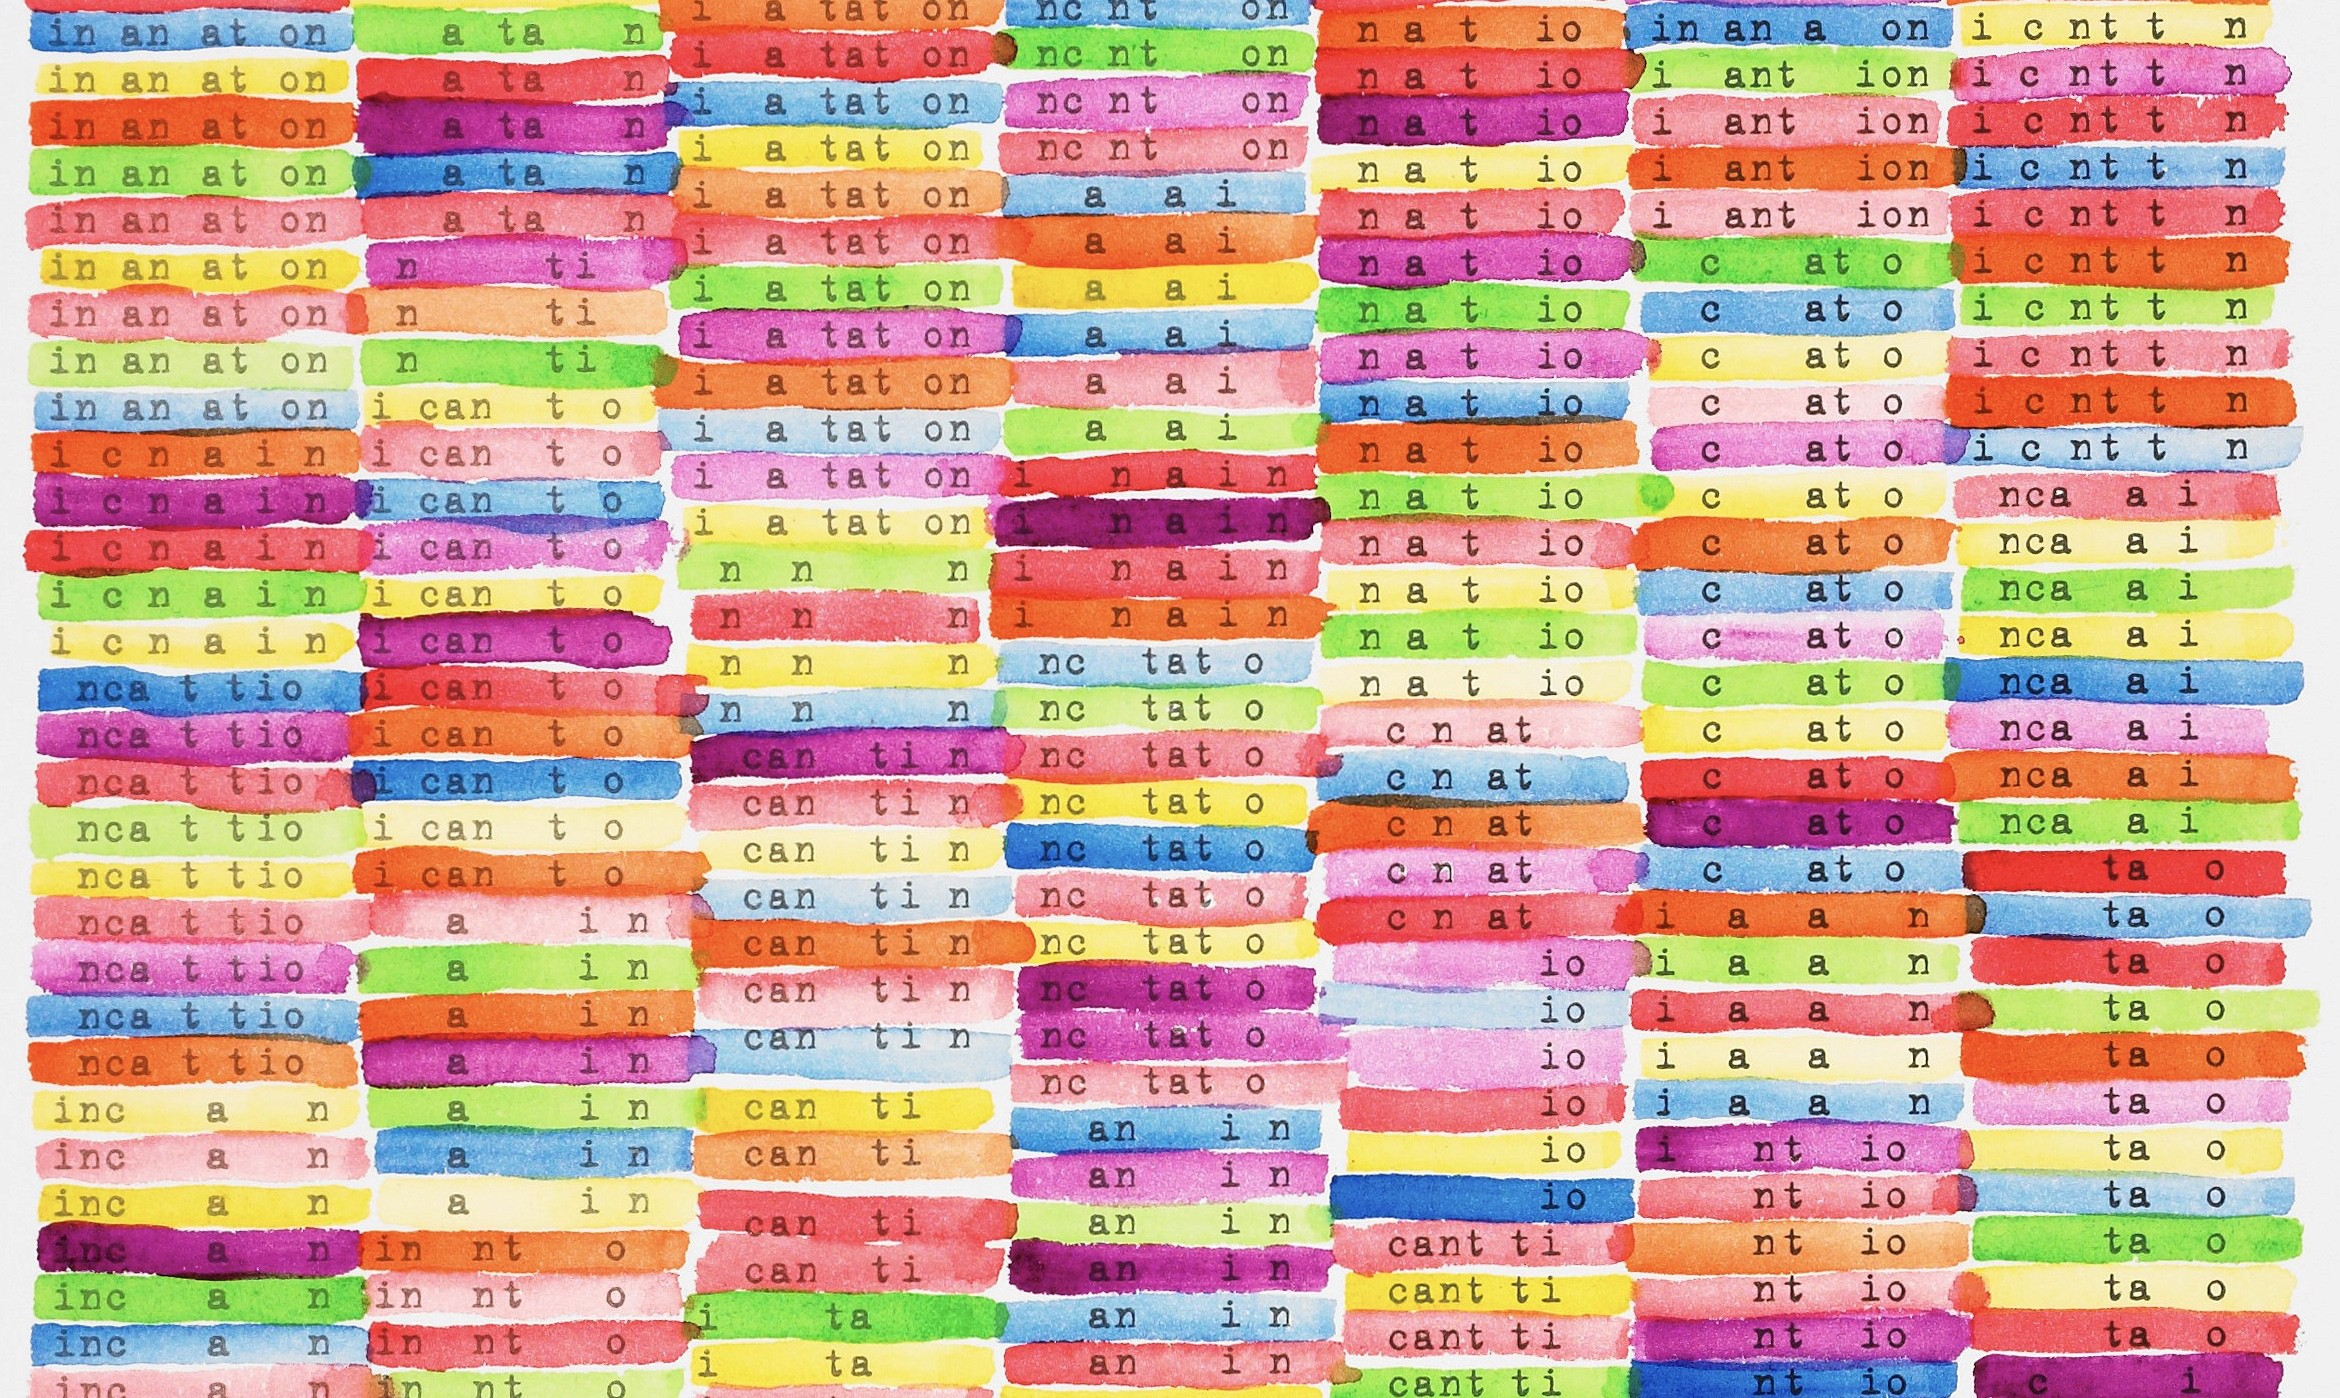
\includegraphics{./images/Incantationfor6voices_scotthelmes2001.jpeg}
\footnote{Incantation for 6 voices Scott helmes, 2001. \href{https://medium.com/minneapolis-institute-of-art/painting-a-picture-with-words-a0a3fef3cf63}{Museum of Minessota}}

L'eco système r s'est enrichi ces dernière années à grande vitesse dans le domaine du traitement du langage naturel, l'objet de ce manuel a pour but d'en donner une synthèse. Sa vocation est pratique même si on y laissera germer quelques considérations plus méthodologiques, voire épistémologiques.
On ouvrira cependant chaque fois que c'est possibles aux questions théoriques et éthiques de ces méthodes. Leur réalisation computationnelle est le fruit souvent d'une longue histoire, au cours de laquelle les linguistes ont semé des idées essentielles qu'ont systématisé les informaticiens.

On soignera la bibliographie de manière synthétique pour en faire un état de l'art essentielet actualisée.

La rédaction de l'ouvrage est mené avec une règle de reproductibilité et de transparence, c'est le pourquoi le choix de ce support et des jeux de données associés.

Il sera dynamique, modifié à mesure de nos cours, séminaires, ateliers et observations des lecteurs.

\hypertarget{cours-et-suxe9minaires}{%
\section{Cours et séminaires}\label{cours-et-suxe9minaires}}

La liste des cours et séminaires où il sera présenté et utilisé.

\begin{itemize}
\tightlist
\item
  Colloque Marketing digital 1-2 septembre 2021
\item
  AFM decembre 2021
\item
  Ed Sorbonne - février 2022
\item
  Dauphine master 204 - octobre 2021
\item
  Master Siren - Dauphine - mai 2022
\item
  Toulouse
\item
  Lille master Data Science
\end{itemize}

\hypertarget{la-structure-du-livre}{%
\section{La structure du livre}\label{la-structure-du-livre}}

L analyse NLP peut être analysée comme un processus qui va de la production jusqu' à la diffusion des analyses. Elle est aussi traversée par des évolutions profondes de méthodes qui ont complexifié au sens formel les modèles initiaux. L'apprentissage submerge le comptage,et les catégorisations\ldots.

Rappelons nous que les modèles de langages désormais distribués par les grands acteurs, comprennent des dizaines, voir des centaines de milliards de paramètres.

Le plan suit une logique qui va du simple au très compliqué, et de l'acquisition des données, de leur traitement et leur modélisation, jusqu'à la propagation\ldots.

\begin{itemize}
\tightlist
\item
  acquisition des données : directe, api et scrapping
\item
  corpus dtm et cooccurence
\item
  AFC et typologie
\item
  l'annotation syntaxique et lexicale
\item
  analyse du sentiment et sa généralisation
\item
  word embedness
\item
  factorial models
\item
  Topic analysis
\item
  ML
\item
  deep learning
\item
  translation : parsceque qu'il faut traiter des corpus multi lingual et que la communication peut aussi etre multilinguales.
\item
  génératives : parce que la prochaine étape c'est quand on appliquera ces méthode sur la productions textuelles des bots.
\end{itemize}

\hypertarget{les-jeux-de-donnuxe9es}{%
\section{Les jeux de données}\label{les-jeux-de-donnuxe9es}}

Au cours du développement, plusieurs cas pratiques - souvent réduit en volume pour rester exemplaires, seront employés. Les donées seront partagées.

En voici la présentation systématique.

\begin{itemize}
\tightlist
\item
  \href{https://www.thetrumparchive.com/}{Trump Twitter Archive} : L'intégralité des tweets de Trump jusqu'à son banissement le 8 Janvier 2021.
\item
  Confinement Jour J
\item
  Citations : un recueil de citations littéraires pour de petits exemples et ponctuer le texte aride d'un peu de littérature et de poésie.
\item
  Trip advisor Polynésie, un extrait d'un corpus établi par Pierre Ghewy et Sebastien de l'UPF
\item
  Airbnb
\item
  Covid
\end{itemize}

disponibles dans le \href{https://benaventc.github.io/NLPBook/}{repositery} avec le code du book. Les amendements et améliorations sont souhaitées et attendues.

\hypertarget{les-ressources}{%
\section{Les ressources}\label{les-ressources}}

Ce \emph{livre} est écrit en \textbf{Markdown} \citep{allaire_rmarkdown_2021} et avec le package \textbf{Bookdown} \citep{R-bookdown}

Le code s'appuie très largement sur \textbf{tidyverse} et emploie largement les ressources de \textbf{ggplot} et \textbf{dplyr} . On recommande au lecteur de consulter donc les ouvrages suivants quand il s'interroge sur la construction des graphiques. On part du parti-pris que les lecteurs ont une connaissance satisfaisantes de ces outils génériques. Une mention particulère doit être faite sur la question du traitement du texte, \textbf{stringr} est aussi un des outils fondamentaux,

\begin{itemize}
\tightlist
\item
  rmardown
\item
  ggplot
\item
  dplyr
\item
  stringer
\end{itemize}

\#\#\#les packages

Les packages seront introduits au fur et à mesure. En voici la liste complète.

\begin{Shaded}
\begin{Highlighting}[]
\NormalTok{knitr}\OperatorTok{::}\NormalTok{opts_chunk}\OperatorTok{$}\KeywordTok{set}\NormalTok{(}\DataTypeTok{echo =} \OtherTok{TRUE}\NormalTok{, }\DataTypeTok{message=}\OtherTok{FALSE}\NormalTok{,}\DataTypeTok{warning=}\OtherTok{FALSE}\NormalTok{)}

\CommentTok{#boite à outils et viz}
\KeywordTok{library}\NormalTok{(tidyverse) }\CommentTok{# inclut ggplot pour la viz, readr et }
\KeywordTok{library}\NormalTok{(cowplot) }\CommentTok{#pour créer des graphiques composés}
\KeywordTok{library}\NormalTok{(ggridges) }\CommentTok{# le joy division touch}
\KeywordTok{library}\NormalTok{(citr)}

\CommentTok{#networks}
\KeywordTok{library}\NormalTok{(igraph)}
\KeywordTok{library}\NormalTok{(ggraph)}

\CommentTok{# Accéder aux données}
\KeywordTok{library}\NormalTok{(rtweet)  }\CommentTok{# une interface efficace pour interroger l'api de Twitter}

\CommentTok{# NLP}
\KeywordTok{library}\NormalTok{(tokenizers)}
\KeywordTok{library}\NormalTok{(quanteda)}
\KeywordTok{library}\NormalTok{(quanteda.textstats)}
\KeywordTok{library}\NormalTok{(quanteda.textplots)}
\KeywordTok{library}\NormalTok{(udpipe) }\CommentTok{#annotation syntaxique}
\KeywordTok{library}\NormalTok{(tidytext)}
\KeywordTok{library}\NormalTok{(cleanNLP) }\CommentTok{#annotation syntaxique}

\CommentTok{#sentiment}
\KeywordTok{library}\NormalTok{(syuzhet)             }\CommentTok{#analyse du sentimeent}
\CommentTok{#mise en page des tableaux}
\KeywordTok{library}\NormalTok{(flextable)}


\CommentTok{#statistiques et modèles}
\KeywordTok{library}\NormalTok{(lme4)}
\KeywordTok{library}\NormalTok{(jtools)}
\KeywordTok{library}\NormalTok{(interactions)}

\CommentTok{#ML}
\KeywordTok{library}\NormalTok{(caret)}

\CommentTok{#graphismes}
\KeywordTok{theme_set}\NormalTok{(}\KeywordTok{theme_bw}\NormalTok{())}


\CommentTok{#palettes}
\KeywordTok{library}\NormalTok{(colorspace) }\CommentTok{#pour les couleurs}

\CommentTok{# chapitre II}
\KeywordTok{library}\NormalTok{(revtools)}
\KeywordTok{library}\NormalTok{(rvest)}
\end{Highlighting}
\end{Shaded}

\hypertarget{disponibilituxe9}{%
\section{Disponibilité}\label{disponibilituxe9}}

L'ensemble du code est disponible \href{https://github.com/BenaventC/NLPBook}{sur github}. A ce stade c'est encore très embryonnaire. Les proches pourrons cependant y voir l'évolution du projet et de la \href{https://benaventc.github.io/NLPBook/}{progression}

\hypertarget{conventions}{%
\section{conventions}\label{conventions}}

Quelques conventions d'écriture du code r

\begin{itemize}
\tightlist
\item
  On appele les dataframes de manière générale \texttt{df}, les tableaux intermédiaires sont appelé systématiquement \texttt{foo}
\item
  Gestion des palettes de couleurs
  ** une couleur :" royalblue"
  ** deux couleurs
  ** 3 à 7 couleurs
\item
  On emploie autant que possible le dialecte tidy.
\item
  Les chunks sont notés X, le chapitre, 01 à n, les jeux. 502 est le second chunk du chapitre 4.
\item
  On commente au maximum les lignes de code pour épargner le corps du texte et le rendre lisible
\end{itemize}

\hypertarget{a-faire}{%
\section{A faire}\label{a-faire}}

todo list :

\begin{itemize}
\tightlist
\item
  insérer un compteur google analytics ( voir \url{https://stackoverflow.com/questions/41376989/how-to-include-google-analytics-in-an-rmarkdown-generated-github-page})
\item
  modifier le titre en haut à gauche
\item
  vérifier le système de références voir ( \url{https://doc.isara.fr/tuto-zothero-5-bibtex-rmarkdown-zotero/})
\item
  Vérifier la publication en pdf
\item
  restructurer le plan
\end{itemize}

\hypertarget{intro}{%
\chapter{Introduction}\label{intro}}

Le texte connaît une double révolution. la première est celle de son système de production, il se produit désormais tant de textes que personne ne peut plus tous les lire, même en réduisant son effort à sa propre sphère d'intérêt et de compétence, la seconde est celle de sa lecture, c'est une lecture conditionnée et recommandée..

La production primaire de textes voit son volume croître exponentiellement. Prenons quelques exemples :

La production se soumet ensuite à ceux qui en contrôlent les flux et en exploitent les contenus, qui les mettent en avant ou les écartent, définissant la composition de ce que chacun va lire. La diffusion de cette production suit des loi puissances, c'est ainsi que la révolution de la lecture est venue avec les moteurs de recherche, et les pratiques de curations (ref), c'est une lecture sélectionnée et digérée par les moteurs de recommandation. (ref).

S'il ne fallait qu'un exemple on pourrait évoquer la transformation radicale de la littérature dite scientifique sur le plan technique. La recherche par mots clés est complétée de plus en plus par des outils de veille, l'indexation a donné naissance à l'immatriculation de la moindre note, les fichiers ont adopté des standards, l'interopérabilité est de mise, le réseau des co-citations est maintenu en temps réel. Les scores qualifient autant les articles que leurs auteurs et les revues qui les accueillent.

Elle risque de ce poursuivre par la production de résumés, la transcription automatique (speech2tex) etc.

Le NLP est au coeur de ces technologies, il se nourrit de plus en plus d'intelligence artificielle. Nous en verrons de nombreux exemple à tout les stades du traitement : identifier la langue, mesurer le sentiment, isoler des sujets.

Le NLP est aussi une nouvelle ressource pour les chercheurs en sciences sociales à la fois par les matériaux empiriques et les méthodes d'analyse. C'est une mouvemenjt qui affecte toutes les shs. L'emballement de la production de texte génère une nouvelle matière d'étude pour le sociologues, le gestionnaire, l'économiste, le psychologue pour n'évoquer que quelques disciplines.

\hypertarget{une-ruxe9flexion-ancienne-et-un-nouveau-champ-muxe9thodologique}{%
\section{Une réflexion ancienne et un nouveau champ méthodologique}\label{une-ruxe9flexion-ancienne-et-un-nouveau-champ-muxe9thodologique}}

On se doit pas se faire aveugler par l'éclat de la nouveauté, les techniques d'aujourd'hui dépendent d'idées semées depuis longtemps dans au moins deux champs disciplinaire la linguistique et l'informatique

Les pratiques et techniques que nous allons étudier ne tombent pas de mars mais résultent de plusieurs flux de pensées qui se croisent se confortent et amène l'energie pour créer un nouveau bras dans le champs immensement étendu de l'étude de la langue et du langage. Et c'ets sans doute par celà qu'il faut commencer. La langue c'est l'ensemble des règle formelles et moins formelle qui constitue une parole, ce qu'on se dit de l'un à l'autre ou de l'un à aux autres. Le langage est la production de cette parole. L'inscription de cette parole par l'écriture constitue le texte. Le miracle du passage de la parole au signe est celui du symbole.

Si dans ce manuel, on choisit de présenter les différentes facettes de ce qui s'appelle TAl, NPL, Text Mining, dans une approche procédurale qui suit les principales étapes du traitement des données. On rendra compte à chaque étape des techniques disponibles, et on illustre d'exemples. Nous suivrons ici une approche plus fidèle au processus de traitement des données, lequel peut connaître une stratégie inférentielle et exploratoire - quelles informations sont utiles au sein d'un corpus de texte -, tout aussi bien qu'une stratégie hypothético-déductive. Nous resterons agnostique sur cette question, restant délibérément à un niveau technique et procédural.

\hypertarget{lhuxe9ritage-linguistique}{%
\subsection{L'héritage linguistique}\label{lhuxe9ritage-linguistique}}

la convergence de deux grands mouvements.

Sans en faire l'histoire minutieuse que ce domaine réclame, nous pouvons au moins rappeler un certains nombre d'étapes et de contributeurs clés.

La langue et le langage sont l'objet d'une interrogation millénaire mais quelques auteurs clés ont mis à jour les idées essentielles qui justifient l'usage des méthodes actuelles. Donnons en un aperçu rapide de manière historique, en bornant un champs de connaissance que nous ne pouvons qu'affleurer.

\begin{itemize}
\tightlist
\item
  les sophistes : plier le langage à ses intérêy est une première sciences du langege qui produit une connaissances des dispositifs les plus efficaces. Par sur que cette displines aient trouvé un chemine de vérité,; mais elle ereste commune, c'est l'oeuvre de la publicité.L
\item
  Saussure : il apporte une idée fondamentale que dans le symbole, le signe et le signifiant sont les deux face d'une même monaiie, qu'il existe une relation entre l'artefact et l'idée. Qu'un signe particulier puisse signifier une idée. c'est un penseur de la correspondance.
\item
  Frith et l'idée distributionnelle. un mot trouve son sens dans ceux qui lui sont le plus associés
\item
  Zipf
\item
  Tesnière et les arbres syntaxiques.
\item
  Chomsky et sa grammaire génératitive. enracinant le phénomène linguistique dans la cortalisation du langage, il apporte une idée forte et structuraliste d'un équivalence des langues.
\item
  Genette et l'intertextualité, le palimpseste. c'est une question de sens, le sens d'un texte vient de ses prédecesssurs de ceux à qui ils se réfèrent. Les textes se parlent l'un l'autre, et ce n'est pas dans leur contenu qu'on trouvera une vérité dans dans le rapport qu'ils établissent avec leur prédecesseur par l'appareil des notes et des bibliographies.
\item
  Austin et l'idée que le langage n'est \^{}pas que communication mais performation . ce qu'on dirt agit sur le monde
\item
  La narrativité
\end{itemize}

\hypertarget{la-tradition-lexicologique}{%
\subsection{la tradition lexicologique}\label{la-tradition-lexicologique}}

le lexique est affaire ancienne, le français est aidé par des expériences les fondamentales : le littré, l'académie française et les dictionnaires des éditeurs. pour étudier un lanage il faut se rapporter à des formes stables, les dictionnaires les fournissent et fournisse les normes pour les coder.

L'idée de quantifier le langage n'est pas nouvelle. Encore moins s'il faut compter les occurences et les cooccurences des mots.Un vaste mouvement s'est formé dans les années soixante autour de la lexicologiue stimulée par l'école française d'analyse de données. Le descendant de ce mouvement se retrouve dans l'excellent iramutek de l'équipe de toulouse, il a été précedé par le fameur Alceste.

Nous y consacrerons un chapitre plein sur le plan technique. Mais il est important de souligner que cette école française de l'analyse textuelle ne se limite pas au comptage. Un logiciel comme trope qui d'ailleurs ne connait aucun équivalent dans l'écosystème que nous allons explorer manifeste aussi cette inventivité.

S'y exprime pleinement la logique distributionnelle.

\hypertarget{la-linguistique-computationnelle}{%
\subsection{la linguistique computationnelle}\label{la-linguistique-computationnelle}}

le frottement de la linguistique et de l'informatique se produit à propos de questions pratiques.

\hypertarget{la-question-de-la-fouille-de-donnuxe9es}{%
\subsubsection{la question de la fouille de données}\label{la-question-de-la-fouille-de-donnuxe9es}}

les nomenclatures

une convergence nécessaire

\hypertarget{la-question-du-classement-des-documents}{%
\subsubsection{la question du classement des documents}\label{la-question-du-classement-des-documents}}

Le monde des bibliothèques et celui de la GED.

\hypertarget{les-facteurs-de-duxe9veloppement}{%
\section{Les facteurs de développement}\label{les-facteurs-de-duxe9veloppement}}

Ces développements sont favorisés par un environnement fertile dont trois facteurs se renforcent mutuellement. Ils conduisent à l'élaboration de nouvelles méthodes.

\begin{itemize}
\tightlist
\item
  la naissance de langue universelle
\item
  l'emergence vaste ensemble de données textuelle
\item
  la naissance d'une communauté épistémique, de pratique et
\end{itemize}

\hypertarget{une-lingua-franca}{%
\subsection{Une lingua franca}\label{une-lingua-franca}}

Le premier est l'expansion de deux langages, proprement statistique pour r et plus généraliste pour Python. Le propre de ces langages est, prenons le cas de r, de permettre d'élaborer des fonctions, dont un ensemble cohérent pour réaliser certaines tâches peut être rassemblé dans une bibliothèque appelée package (et chargé par library(nomdupackage)). On dispose désormais de milliers de packages (17 788 sur le CRAN) destinés à résoudre un nombre incalculable de tâches.

\begin{figure}
\centering
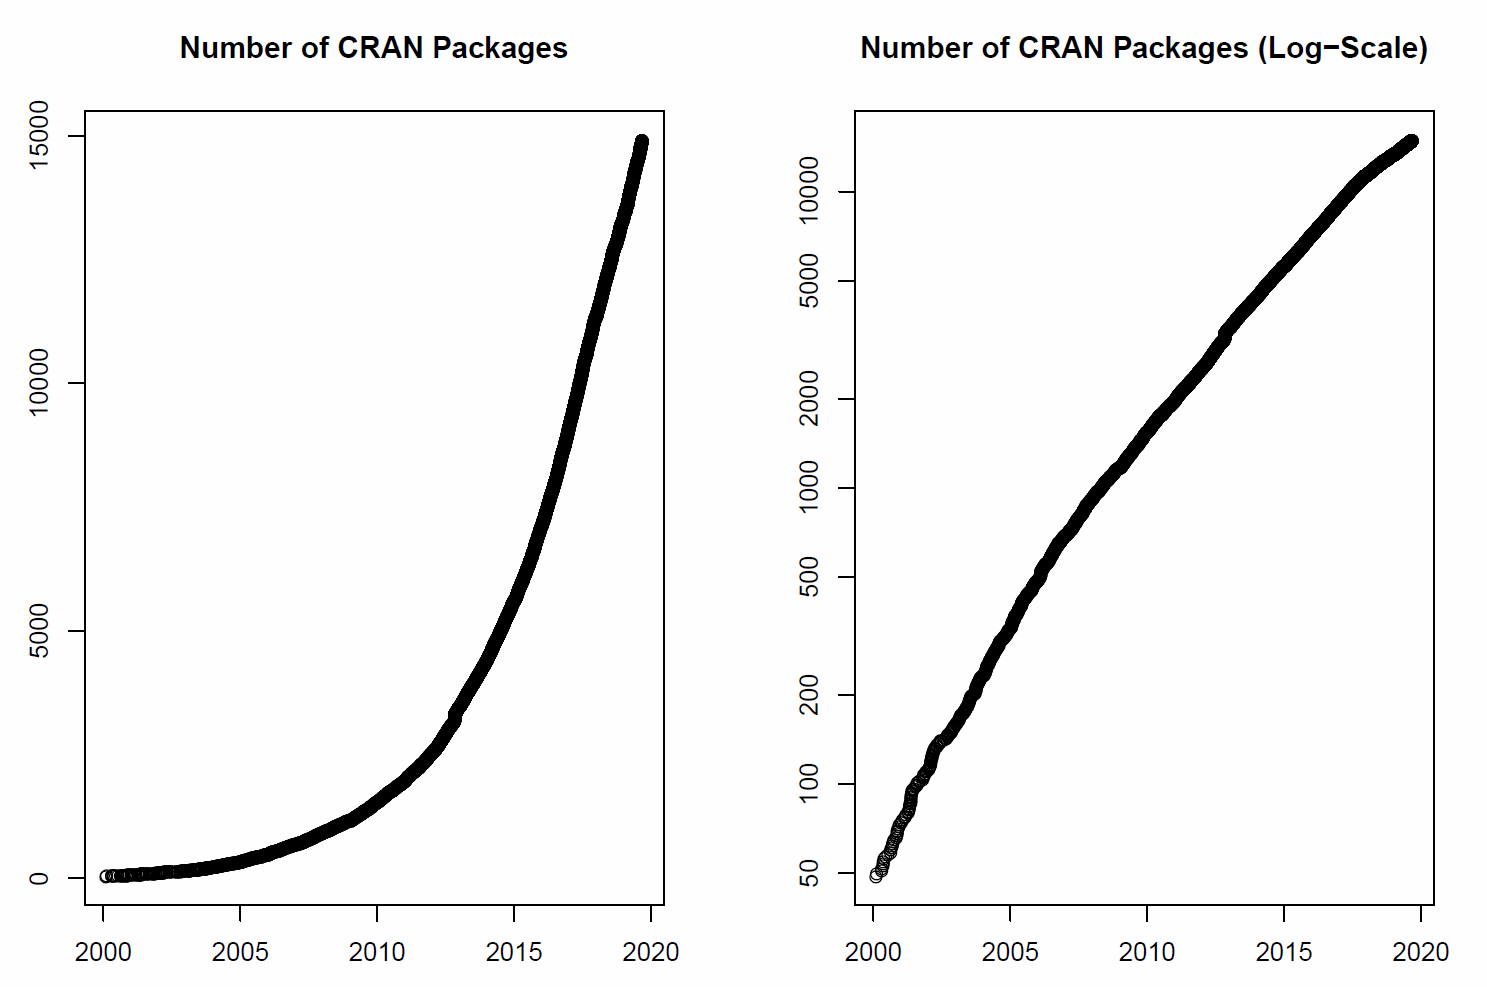
\includegraphics{number_CRAN_packages.png}
\caption{hornik}
\end{figure}

Coder une analyse revient ainsi à jouer avec un immense jeu de lego, dont de nombreuses pièces sont déjà pré-assemblées. D'un point de vue pratique, les lignes d'écriture sont fortement simplifiées permettant à un chercheur sans grande compétence de codage d'effectuer simplement des opérations complexes. En retour, cette facilitation de l'analyse abonde le stock de solutions.

\hypertarget{la-multiplication-des-sources-de-donnuxe9es.}{%
\subsection{La multiplication des sources de données.}\label{la-multiplication-des-sources-de-donnuxe9es.}}

Le troisième est la multiplication des sources de données et leur facilité d'accès.

\begin{itemize}
\tightlist
\item
  le contenu écrit des réseaux sociaux
\item
  les rapports d'activités des entreprises,
\item
  les compte-rendu archivé de réunion
\item
  Les avis des consommateurs sur les catalogues de produit
\item
  Les articles et les revues scientifiques
\item
  Même les livres
\end{itemize}

Les plus évidentes sont proposées par les bases d'articles de presse telles qu' presseurop ou factiva. Les bases de données bibliographiques sont dans la même veine particuièrement intéressante et pensée pour ces usages.

Les données privées, et en particulier celles des réseaux sociaux, même si un péage doit être payé pour accéder aux APIs, popularisent le traitement de données massives.

Les forums et sites d'avis de consommateurs sont pour les sociologues de la consommation et les specialiste du comportement de consommation une ressource directe et précieuses.

Le mouvement des données ouvertes (open data) proposent et facilitent l'accès à des milliers de corps de données : grand débat.

\hypertarget{une-communautuxe9}{%
\subsection{Une communauté}\label{une-communautuxe9}}

Le second facteur de développement , intimement lié au premier, est la constitution d'une large communauté de développeurs et d'utilisateurs qui se retrouvent aujourd'hui dans des plateformes diverses. Le savoir, autrement dit des codes commentés se trouvent dans une varété importante de lieux :

\begin{itemize}
\tightlist
\item
  Des plateformes de dépots telle que Github qui rassemblent une trentaine de millions de developpeurs et datascientits.\\
\item
  Des plateformes de Q\&A (question et réponses) telles que \href{}{Stalk Over Flow},
\item
  Des tutoriaux de toute sortes
\item
  Des blogs ou des fédération de blog de blogs (BloggeR),
\item
  Des revues (Journal of Statistical Software) et de bookdown.
\end{itemize}

Des ressources abondantes sont ainsi disponibles et facilitent la formation des chercheurs et des data scientists et la résolution de leurs problèmes pratiques, quiconque n'arrive pas à résoudre un problème a une bonne chance de trouver la solution d'un autre, à un degré de circonstance près. Elles sont d'autant plus utiles que certaines règles ou conventions s'imposent pour fluidifier l'échange.

La principale est celle de l'exemple reproductible.

La seconde est le maintien d'une éthique du partage qui encourage à partager le code, et dont une littérature importante étudie l'effet positif sur les performances économiques et la durabilité {[}rauter{]}. Les externalités de réseaux y sont fortes

Toutes les conditions sont réunies pour engendrer une effervescence créative. Python ou r, sont dans cet univers en rapide expansion, les langues véhiculaires qui favorise une innovation constante. Les statistiques de github en témoigne : près de 50 millions d'utiliseurs, 128 millions de " repositories" et 23 millions de propriétaires.

\begin{figure}
\centering
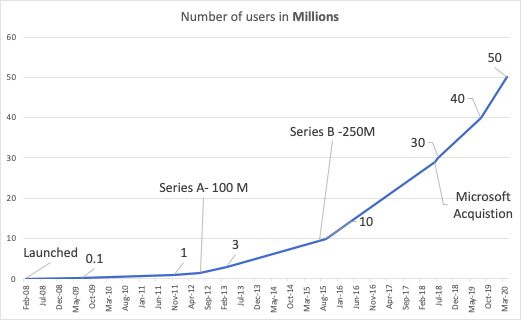
\includegraphics{github.png}
\caption{source}
\end{figure}

voir aussi
\url{https://towardsdatascience.com/githubs-path-to-128m-public-repositories-f6f656ab56b1}

\hypertarget{de-nouvelles-muxe9thodologies-pour-les-sciences-sociales}{%
\section{De nouvelles méthodologies pour les sciences sociales}\label{de-nouvelles-muxe9thodologies-pour-les-sciences-sociales}}

Pour les chercheurs en sciences sociales (et en premier lieu pour les chercheurs en gestion où toutes les sciences sociales se croisent) cette révolution textuelle offre de nouvelles opportunités d'obtenir et d'analyser des données pour vérifier ses hypothèses et mener son enquête. Ce sont de nouveaux terrains, de nouvelles méthodes et un nouvel objet de recherche.

\begin{itemize}
\item
  Nouveaux terrains : La multiplication des sources de données, associée à leur normalisation rencontre une multiplication de techniques provenant de mulpliples discplinaire et qui convergent dans un langage commun. . production abondante d'avis de consommateurs, de discours de dirigeants, de compte-rendus de conseils, d'articles techniques,la linguistique computationnelle, de la fouille de données, des moteurs de recommandation, de la traduction automatique, et des ressources nouvelles et précieuses pour traiter l'abondance des données
\item
  Nouvelles méthodes : Un nouveau paradigme méthodologique se construit à la croisée de données abondantes et de techniques de traitement intelligentes. Il permet d'aller plus loin que l'analyse lexicale traditionnelle en incorporant des éléments syntaxiques, sémantiques, et pragmatiques, proposés par l'ensemble des outils des techniques de traitement du langage naturel. Il se dessine surtout une nouvelle approche méthodologique qui prend place entre l'analyse qualitative, et les traditionnelles enquêtes par questionnaires capables de traiter des corpus d'une taille inédite. Le travail de \citep{humphreys_automated_2018} en donne une première synthèse dans le cadre d'un processus qui s'articule autour des différentes phases d'une recherche : la formulation de la question de recherche, la définition des construits, la récolte des données, l'opérationnalisation des construits, et enfin l'interprétation, l'analyse et la validation des résultats obtenus.
\item
  Un nouvel objet : on pourrait croire qu'avec des données massives et des techniques ``intelligente'' on assiste à un retour du positivisme qui bénéficierait enfin des instruments de mesure et de calculs qui ont permis aux les chercheur plus proches de la matière des succès majeurs. Sans doute, l'administration de la preuve va être faciliter par ces techniques et encourager l'evidence based policy (REF) et résoudre en partie la crise de la réplication et de la reproductibilité. Mais à mesure que ce développe l'appareillage de méthode et de données, moins on peut supposer que l'observateur est neutre. Les téléscopes géants, les synchrotron, n'affecte ni les galaxies lointaines ni les atomes proches. Le propre des données que l'ont est amené à étudier est de résulter de la confrontation d'un système d'observation (certains préfèrent de parler de surveillance), et d'un agent qui a des buts, une connaissance, et des ressources. Le dispositif de mesure est en lui-même performatif. L'exemple le plus évident est celui des systèmes de notation, qui sous prétexte de transparence donne la distribution des répondants précédents. L'agent qui va noter choisit la valeur en fonction d'une norme apparente - la note majoritaire- et de sa propre intention - se manifester ou se confondre à la foule.
\end{itemize}

Pour se donner une idée plus précise de ce mouvement, examinons quelques publications récentes dans les champs qui nous concernent.

\hypertarget{sociologie-et-histoire}{%
\subsection{Sociologie et histoire}\label{sociologie-et-histoire}}

classes sociales avec word to vec en sociologie \citep{kozlowski_geometry_2019}.

L'article révolution française {[}PNAS)

On citera cependant jean-baptiste Coulmont et son obstination à étudier les entités nommées, prénoms et autres marqueurs culturels de l'identité et des classes.

\hypertarget{psychologie}{%
\subsection{Psychologie}\label{psychologie}}

Très tôt la psychogie s'est intéressée au langage, pas seulement comme produit des processus psychologiques, mais comme expression de ceux-ci.

Dans le champs de la psychologie de l'éducation et avec une forte motivation scientiste, dès les années 60 s'est posée la question de la mesure de la difficulté d'un texte pour un niveau d'éducation donné. La mesure de la lisibilité des texte s'est développée profitant à d'autre secteurs tels que ceux de la propagande. Dans cette même perspective, la richesse lexicographique comme représentant les compétences a a son tour développé de nouvelles instrumentations.

James W. Pennebaker a développé son approche à partir de l'étude des traumas; donnant une grande importance à la production discursive des patients. Sa contribution majeure est l'établissement d'un ensemble de dictionnaires destinés à mesurer des caractéristiques du discours. Un instrument qu'on présentatera dans les chapitre 7 (à vérifier). Auteur en 2011 d'un livre s'intéressant à l'usage des petits mots. Son approche se poursuit en psychiatrie avec l'analyse des troubles du langage, et a connu un coup d'éclat avec la demonstration que l'analyse des messages sur les réseaux sociaux comme facebook permet de détecter des risques de depression.

\hypertarget{management}{%
\subsection{Management}\label{management}}

La finance et l'analyse du sentiment

Dans le champ du management, on trouvera des synthèses pour la recherche en éthique \citep{lock_quantitative_2015}, en comportement du consommateur {[}\citet{humphreys_automated_2018} en management public \citep{anastasopoulos_computational_2017} ou en organisation \citep{kobayashi_text_2018} ,

\hypertarget{economie}{%
\subsection{Economie}\label{economie}}

economie des brevets
intervention des institutions

\hypertarget{conclusion}{%
\section{Conclusion}\label{conclusion}}

des techniques

des méthodes

\hypertarget{constitution-du-corpus}{%
\chapter{Constitution du corpus}\label{constitution-du-corpus}}

\textbf{Objectifs du chapitre : } ** explorer différente techniques de collectes de données : exploitation de bases textuelles, méthodes de scrapping, APIS, extraction de document pdf, extration de texte dans des images, et une perspective oral avec les techniques de speech2 tex.**

La constitution d'un corpus est la première étape d'un projet NLP. Il se définit d'abord par la constitution d'une collection de textes dont la provenance est la nature peut être diverse. Dans ce chapitre on va examiner plusieurs techniques de collecte, et on conclue avec quelques réflexions que la questions de la constitution de l'échantillon.

\begin{itemize}
\tightlist
\item
  L'exploitation de bases textuelles
\item
  Les méthodes de scrapping
\item
  Le recours aux APIs
\item
  La collection de document pas que textuels
\item
  Les sources orales
\end{itemize}

et on conclue avec quelques réflexions que la questions de la constitution de l'échantillon.

\hypertarget{lexploitation-de-base-de-donnuxe9es-textuelles}{%
\section{L'exploitation de base de données textuelles}\label{lexploitation-de-base-de-donnuxe9es-textuelles}}

On commence par un exemple simple en utilisant la base \href{http://www.europresse.com/fr/}{europresse}. l'objectif est de constituer un fichier de références bibliographiques, exploitable via r.

Dans europresse , nous avons fait une recherche sur les articles comprenant le terme " vaccination" dans la presse nationale françaises, constituées de 14 titres. On retient les 150 derniers articles au 16 Juillet 2021.

On utilise \href{https://revtools.net/data.html\#importing-to-r}{revtools} pour sa fonction d'importation des fichier *.RIS et de transformation en data frame,

\begin{Shaded}
\begin{Highlighting}[]
\KeywordTok{library}\NormalTok{(revtools)}


\NormalTok{df <-}\StringTok{ }\KeywordTok{read_bibliography}\NormalTok{(}\KeywordTok{iconv}\NormalTok{(}\StringTok{"./data/20210719013820.ris"}\NormalTok{))}

\KeywordTok{flextable}\NormalTok{(}\KeywordTok{head}\NormalTok{(df,}\DecValTok{3}\NormalTok{))}
\end{Highlighting}
\end{Shaded}

\providecommand{\docline}[3]{\noalign{\global\setlength{\arrayrulewidth}{#1}}\arrayrulecolor[HTML]{#2}\cline{#3}}

\setlength{\tabcolsep}{2pt}

\renewcommand*{\arraystretch}{1.5}

\begin{longtable}[c]{|p{0.75in}|p{0.75in}|p{0.75in}|p{0.75in}|p{0.75in}|p{0.75in}|p{0.75in}|p{0.75in}|p{0.75in}|p{0.75in}|p{0.75in}|p{0.75in}}



\hhline{>{\arrayrulecolor[HTML]{666666}\global\arrayrulewidth=2pt}->{\arrayrulecolor[HTML]{666666}\global\arrayrulewidth=2pt}->{\arrayrulecolor[HTML]{666666}\global\arrayrulewidth=2pt}->{\arrayrulecolor[HTML]{666666}\global\arrayrulewidth=2pt}->{\arrayrulecolor[HTML]{666666}\global\arrayrulewidth=2pt}->{\arrayrulecolor[HTML]{666666}\global\arrayrulewidth=2pt}->{\arrayrulecolor[HTML]{666666}\global\arrayrulewidth=2pt}->{\arrayrulecolor[HTML]{666666}\global\arrayrulewidth=2pt}->{\arrayrulecolor[HTML]{666666}\global\arrayrulewidth=2pt}->{\arrayrulecolor[HTML]{666666}\global\arrayrulewidth=2pt}->{\arrayrulecolor[HTML]{666666}\global\arrayrulewidth=2pt}->{\arrayrulecolor[HTML]{666666}\global\arrayrulewidth=2pt}-}

\multicolumn{1}{!{\color[HTML]{000000}\vrule width 0pt}>{\raggedright}p{\dimexpr 0.75in+0\tabcolsep+0\arrayrulewidth}}{\fontsize{11}{11}\selectfont{\textcolor[HTML]{000000}{\global\setmainfont{Arial}label}}} & \multicolumn{1}{!{\color[HTML]{000000}\vrule width 0pt}>{\raggedright}p{\dimexpr 0.75in+0\tabcolsep+0\arrayrulewidth}}{\fontsize{11}{11}\selectfont{\textcolor[HTML]{000000}{\global\setmainfont{Arial}type}}} & \multicolumn{1}{!{\color[HTML]{000000}\vrule width 0pt}>{\raggedright}p{\dimexpr 0.75in+0\tabcolsep+0\arrayrulewidth}}{\fontsize{11}{11}\selectfont{\textcolor[HTML]{000000}{\global\setmainfont{Arial}title}}} & \multicolumn{1}{!{\color[HTML]{000000}\vrule width 0pt}>{\raggedright}p{\dimexpr 0.75in+0\tabcolsep+0\arrayrulewidth}}{\fontsize{11}{11}\selectfont{\textcolor[HTML]{000000}{\global\setmainfont{Arial}author}}} & \multicolumn{1}{!{\color[HTML]{000000}\vrule width 0pt}>{\raggedright}p{\dimexpr 0.75in+0\tabcolsep+0\arrayrulewidth}}{\fontsize{11}{11}\selectfont{\textcolor[HTML]{000000}{\global\setmainfont{Arial}abstract}}} & \multicolumn{1}{!{\color[HTML]{000000}\vrule width 0pt}>{\raggedright}p{\dimexpr 0.75in+0\tabcolsep+0\arrayrulewidth}}{\fontsize{11}{11}\selectfont{\textcolor[HTML]{000000}{\global\setmainfont{Arial}journal}}} & \multicolumn{1}{!{\color[HTML]{000000}\vrule width 0pt}>{\raggedright}p{\dimexpr 0.75in+0\tabcolsep+0\arrayrulewidth}}{\fontsize{11}{11}\selectfont{\textcolor[HTML]{000000}{\global\setmainfont{Arial}pages}}} & \multicolumn{1}{!{\color[HTML]{000000}\vrule width 0pt}>{\raggedright}p{\dimexpr 0.75in+0\tabcolsep+0\arrayrulewidth}}{\fontsize{11}{11}\selectfont{\textcolor[HTML]{000000}{\global\setmainfont{Arial}year}}} & \multicolumn{1}{!{\color[HTML]{000000}\vrule width 0pt}>{\raggedright}p{\dimexpr 0.75in+0\tabcolsep+0\arrayrulewidth}}{\fontsize{11}{11}\selectfont{\textcolor[HTML]{000000}{\global\setmainfont{Arial}language}}} & \multicolumn{1}{!{\color[HTML]{000000}\vrule width 0pt}>{\raggedright}p{\dimexpr 0.75in+0\tabcolsep+0\arrayrulewidth}}{\fontsize{11}{11}\selectfont{\textcolor[HTML]{000000}{\global\setmainfont{Arial}url}}} & \multicolumn{1}{!{\color[HTML]{000000}\vrule width 0pt}>{\raggedright}p{\dimexpr 0.75in+0\tabcolsep+0\arrayrulewidth}}{\fontsize{11}{11}\selectfont{\textcolor[HTML]{000000}{\global\setmainfont{Arial}DA}}} & \multicolumn{1}{!{\color[HTML]{000000}\vrule width 0pt}>{\raggedright}p{\dimexpr 0.75in+0\tabcolsep+0\arrayrulewidth}!{\color[HTML]{000000}\vrule width 0pt}}{\fontsize{11}{11}\selectfont{\textcolor[HTML]{000000}{\global\setmainfont{Arial}OP}}} \\

\noalign{\global\setlength{\arrayrulewidth}{2pt}}\arrayrulecolor[HTML]{666666}\cline{1-12}

\endfirsthead

\hhline{>{\arrayrulecolor[HTML]{666666}\global\arrayrulewidth=2pt}->{\arrayrulecolor[HTML]{666666}\global\arrayrulewidth=2pt}->{\arrayrulecolor[HTML]{666666}\global\arrayrulewidth=2pt}->{\arrayrulecolor[HTML]{666666}\global\arrayrulewidth=2pt}->{\arrayrulecolor[HTML]{666666}\global\arrayrulewidth=2pt}->{\arrayrulecolor[HTML]{666666}\global\arrayrulewidth=2pt}->{\arrayrulecolor[HTML]{666666}\global\arrayrulewidth=2pt}->{\arrayrulecolor[HTML]{666666}\global\arrayrulewidth=2pt}->{\arrayrulecolor[HTML]{666666}\global\arrayrulewidth=2pt}->{\arrayrulecolor[HTML]{666666}\global\arrayrulewidth=2pt}->{\arrayrulecolor[HTML]{666666}\global\arrayrulewidth=2pt}->{\arrayrulecolor[HTML]{666666}\global\arrayrulewidth=2pt}-}

\multicolumn{1}{!{\color[HTML]{000000}\vrule width 0pt}>{\raggedright}p{\dimexpr 0.75in+0\tabcolsep+0\arrayrulewidth}}{\fontsize{11}{11}\selectfont{\textcolor[HTML]{000000}{\global\setmainfont{Arial}label}}} & \multicolumn{1}{!{\color[HTML]{000000}\vrule width 0pt}>{\raggedright}p{\dimexpr 0.75in+0\tabcolsep+0\arrayrulewidth}}{\fontsize{11}{11}\selectfont{\textcolor[HTML]{000000}{\global\setmainfont{Arial}type}}} & \multicolumn{1}{!{\color[HTML]{000000}\vrule width 0pt}>{\raggedright}p{\dimexpr 0.75in+0\tabcolsep+0\arrayrulewidth}}{\fontsize{11}{11}\selectfont{\textcolor[HTML]{000000}{\global\setmainfont{Arial}title}}} & \multicolumn{1}{!{\color[HTML]{000000}\vrule width 0pt}>{\raggedright}p{\dimexpr 0.75in+0\tabcolsep+0\arrayrulewidth}}{\fontsize{11}{11}\selectfont{\textcolor[HTML]{000000}{\global\setmainfont{Arial}author}}} & \multicolumn{1}{!{\color[HTML]{000000}\vrule width 0pt}>{\raggedright}p{\dimexpr 0.75in+0\tabcolsep+0\arrayrulewidth}}{\fontsize{11}{11}\selectfont{\textcolor[HTML]{000000}{\global\setmainfont{Arial}abstract}}} & \multicolumn{1}{!{\color[HTML]{000000}\vrule width 0pt}>{\raggedright}p{\dimexpr 0.75in+0\tabcolsep+0\arrayrulewidth}}{\fontsize{11}{11}\selectfont{\textcolor[HTML]{000000}{\global\setmainfont{Arial}journal}}} & \multicolumn{1}{!{\color[HTML]{000000}\vrule width 0pt}>{\raggedright}p{\dimexpr 0.75in+0\tabcolsep+0\arrayrulewidth}}{\fontsize{11}{11}\selectfont{\textcolor[HTML]{000000}{\global\setmainfont{Arial}pages}}} & \multicolumn{1}{!{\color[HTML]{000000}\vrule width 0pt}>{\raggedright}p{\dimexpr 0.75in+0\tabcolsep+0\arrayrulewidth}}{\fontsize{11}{11}\selectfont{\textcolor[HTML]{000000}{\global\setmainfont{Arial}year}}} & \multicolumn{1}{!{\color[HTML]{000000}\vrule width 0pt}>{\raggedright}p{\dimexpr 0.75in+0\tabcolsep+0\arrayrulewidth}}{\fontsize{11}{11}\selectfont{\textcolor[HTML]{000000}{\global\setmainfont{Arial}language}}} & \multicolumn{1}{!{\color[HTML]{000000}\vrule width 0pt}>{\raggedright}p{\dimexpr 0.75in+0\tabcolsep+0\arrayrulewidth}}{\fontsize{11}{11}\selectfont{\textcolor[HTML]{000000}{\global\setmainfont{Arial}url}}} & \multicolumn{1}{!{\color[HTML]{000000}\vrule width 0pt}>{\raggedright}p{\dimexpr 0.75in+0\tabcolsep+0\arrayrulewidth}}{\fontsize{11}{11}\selectfont{\textcolor[HTML]{000000}{\global\setmainfont{Arial}DA}}} & \multicolumn{1}{!{\color[HTML]{000000}\vrule width 0pt}>{\raggedright}p{\dimexpr 0.75in+0\tabcolsep+0\arrayrulewidth}!{\color[HTML]{000000}\vrule width 0pt}}{\fontsize{11}{11}\selectfont{\textcolor[HTML]{000000}{\global\setmainfont{Arial}OP}}} \\

\noalign{\global\setlength{\arrayrulewidth}{2pt}}\arrayrulecolor[HTML]{666666}\cline{1-12}\endhead



\multicolumn{1}{!{\color[HTML]{000000}\vrule width 0pt}>{\raggedright}p{\dimexpr 0.75in+0\tabcolsep+0\arrayrulewidth}}{\fontsize{11}{11}\selectfont{\textcolor[HTML]{000000}{\global\setmainfont{Arial}By.Cecilia.Kang\_2021\_TheNewYorTim}}} & \multicolumn{1}{!{\color[HTML]{000000}\vrule width 0pt}>{\raggedright}p{\dimexpr 0.75in+0\tabcolsep+0\arrayrulewidth}}{\fontsize{11}{11}\selectfont{\textcolor[HTML]{000000}{\global\setmainfont{Arial}NEWS}}} & \multicolumn{1}{!{\color[HTML]{000000}\vrule width 0pt}>{\raggedright}p{\dimexpr 0.75in+0\tabcolsep+0\arrayrulewidth}}{\fontsize{11}{11}\selectfont{\textcolor[HTML]{000000}{\global\setmainfont{Arial}Facebook\ Says\ Biden\ Is\ Scapegoating\ Over\ Vaccine\ Falsehoods}}} & \multicolumn{1}{!{\color[HTML]{000000}\vrule width 0pt}>{\raggedright}p{\dimexpr 0.75in+0\tabcolsep+0\arrayrulewidth}}{\fontsize{11}{11}\selectfont{\textcolor[HTML]{000000}{\global\setmainfont{Arial}By\ Cecilia\ Kang}}} & \multicolumn{1}{!{\color[HTML]{000000}\vrule width 0pt}>{\raggedright}p{\dimexpr 0.75in+0\tabcolsep+0\arrayrulewidth}}{\fontsize{11}{11}\selectfont{\textcolor[HTML]{000000}{\global\setmainfont{Arial}The\ social\ network\ and\ the\ Biden\ administration\ have\ engaged\ in\ an\ increasingly\ rancorous\ war\ of\ words\ over\ the\ issue\ of\ vaccine\ misinformation.\ WASHINGTON\ --\ Facebook\ and\ the\ Biden\ administration\ engaged\ in\ an\ ...}}} & \multicolumn{1}{!{\color[HTML]{000000}\vrule width 0pt}>{\raggedright}p{\dimexpr 0.75in+0\tabcolsep+0\arrayrulewidth}}{\fontsize{11}{11}\selectfont{\textcolor[HTML]{000000}{\global\setmainfont{Arial}The\ New\ York\ Times}}} & \multicolumn{1}{!{\color[HTML]{000000}\vrule width 0pt}>{\raggedright}p{\dimexpr 0.75in+0\tabcolsep+0\arrayrulewidth}}{\fontsize{11}{11}\selectfont{\textcolor[HTML]{000000}{\global\setmainfont{Arial}B\ 3}}} & \multicolumn{1}{!{\color[HTML]{000000}\vrule width 0pt}>{\raggedright}p{\dimexpr 0.75in+0\tabcolsep+0\arrayrulewidth}}{\fontsize{11}{11}\selectfont{\textcolor[HTML]{000000}{\global\setmainfont{Arial}2021}}} & \multicolumn{1}{!{\color[HTML]{000000}\vrule width 0pt}>{\raggedright}p{\dimexpr 0.75in+0\tabcolsep+0\arrayrulewidth}}{\fontsize{11}{11}\selectfont{\textcolor[HTML]{000000}{\global\setmainfont{Arial}English}}} & \multicolumn{1}{!{\color[HTML]{000000}\vrule width 0pt}>{\raggedright}p{\dimexpr 0.75in+0\tabcolsep+0\arrayrulewidth}}{\fontsize{11}{11}\selectfont{\textcolor[HTML]{000000}{\global\setmainfont{Arial}https://nouveau.europresse.com/Link/PARIS10T\_1/news\%c2\%b720210719\%c2\%b7NY\%c2\%b7721611}}} & \multicolumn{1}{!{\color[HTML]{000000}\vrule width 0pt}>{\raggedright}p{\dimexpr 0.75in+0\tabcolsep+0\arrayrulewidth}}{\fontsize{11}{11}\selectfont{\textcolor[HTML]{000000}{\global\setmainfont{Arial}19/07/2021}}} & \multicolumn{1}{!{\color[HTML]{000000}\vrule width 0pt}>{\raggedright}p{\dimexpr 0.75in+0\tabcolsep+0\arrayrulewidth}!{\color[HTML]{000000}\vrule width 0pt}}{\fontsize{11}{11}\selectfont{\textcolor[HTML]{000000}{\global\setmainfont{Arial}19/07/2021}}} \\





\multicolumn{1}{!{\color[HTML]{000000}\vrule width 0pt}>{\raggedright}p{\dimexpr 0.75in+0\tabcolsep+0\arrayrulewidth}}{\fontsize{11}{11}\selectfont{\textcolor[HTML]{000000}{\global\setmainfont{Arial}By.Matt.Stevens\_2021\_TheNewYorTim}}} & \multicolumn{1}{!{\color[HTML]{000000}\vrule width 0pt}>{\raggedright}p{\dimexpr 0.75in+0\tabcolsep+0\arrayrulewidth}}{\fontsize{11}{11}\selectfont{\textcolor[HTML]{000000}{\global\setmainfont{Arial}NEWS}}} & \multicolumn{1}{!{\color[HTML]{000000}\vrule width 0pt}>{\raggedright}p{\dimexpr 0.75in+0\tabcolsep+0\arrayrulewidth}}{\fontsize{11}{11}\selectfont{\textcolor[HTML]{000000}{\global\setmainfont{Arial}Rules\ for\ Audiences\ Can\ Spin\ Heads}}} & \multicolumn{1}{!{\color[HTML]{000000}\vrule width 0pt}>{\raggedright}p{\dimexpr 0.75in+0\tabcolsep+0\arrayrulewidth}}{\fontsize{11}{11}\selectfont{\textcolor[HTML]{000000}{\global\setmainfont{Arial}By\ Matt\ Stevens}}} & \multicolumn{1}{!{\color[HTML]{000000}\vrule width 0pt}>{\raggedright}p{\dimexpr 0.75in+0\tabcolsep+0\arrayrulewidth}}{\fontsize{11}{11}\selectfont{\textcolor[HTML]{000000}{\global\setmainfont{Arial}Vaccination\ and\ mask\ requirements\ vary\ by\ venue.\ It's\ a\ weird\ pandemic\ summer\ for\ the\ performing\ arts.\ During\ its\ preview\ performances\ in\ June,\ New\ York\ Classical\ Theater\ was\ allowed\ to\ put\ ...}}} & \multicolumn{1}{!{\color[HTML]{000000}\vrule width 0pt}>{\raggedright}p{\dimexpr 0.75in+0\tabcolsep+0\arrayrulewidth}}{\fontsize{11}{11}\selectfont{\textcolor[HTML]{000000}{\global\setmainfont{Arial}The\ New\ York\ Times}}} & \multicolumn{1}{!{\color[HTML]{000000}\vrule width 0pt}>{\raggedright}p{\dimexpr 0.75in+0\tabcolsep+0\arrayrulewidth}}{\fontsize{11}{11}\selectfont{\textcolor[HTML]{000000}{\global\setmainfont{Arial}C\ 1}}} & \multicolumn{1}{!{\color[HTML]{000000}\vrule width 0pt}>{\raggedright}p{\dimexpr 0.75in+0\tabcolsep+0\arrayrulewidth}}{\fontsize{11}{11}\selectfont{\textcolor[HTML]{000000}{\global\setmainfont{Arial}2021}}} & \multicolumn{1}{!{\color[HTML]{000000}\vrule width 0pt}>{\raggedright}p{\dimexpr 0.75in+0\tabcolsep+0\arrayrulewidth}}{\fontsize{11}{11}\selectfont{\textcolor[HTML]{000000}{\global\setmainfont{Arial}English}}} & \multicolumn{1}{!{\color[HTML]{000000}\vrule width 0pt}>{\raggedright}p{\dimexpr 0.75in+0\tabcolsep+0\arrayrulewidth}}{\fontsize{11}{11}\selectfont{\textcolor[HTML]{000000}{\global\setmainfont{Arial}https://nouveau.europresse.com/Link/PARIS10T\_1/news\%c2\%b720210719\%c2\%b7NY\%c2\%b7456420}}} & \multicolumn{1}{!{\color[HTML]{000000}\vrule width 0pt}>{\raggedright}p{\dimexpr 0.75in+0\tabcolsep+0\arrayrulewidth}}{\fontsize{11}{11}\selectfont{\textcolor[HTML]{000000}{\global\setmainfont{Arial}19/07/2021}}} & \multicolumn{1}{!{\color[HTML]{000000}\vrule width 0pt}>{\raggedright}p{\dimexpr 0.75in+0\tabcolsep+0\arrayrulewidth}!{\color[HTML]{000000}\vrule width 0pt}}{\fontsize{11}{11}\selectfont{\textcolor[HTML]{000000}{\global\setmainfont{Arial}19/07/2021}}} \\





\multicolumn{1}{!{\color[HTML]{000000}\vrule width 0pt}>{\raggedright}p{\dimexpr 0.75in+0\tabcolsep+0\arrayrulewidth}}{\fontsize{11}{11}\selectfont{\textcolor[HTML]{000000}{\global\setmainfont{Arial}By.Lisa.Lerer\_2021\_TheNewYorTim}}} & \multicolumn{1}{!{\color[HTML]{000000}\vrule width 0pt}>{\raggedright}p{\dimexpr 0.75in+0\tabcolsep+0\arrayrulewidth}}{\fontsize{11}{11}\selectfont{\textcolor[HTML]{000000}{\global\setmainfont{Arial}NEWS}}} & \multicolumn{1}{!{\color[HTML]{000000}\vrule width 0pt}>{\raggedright}p{\dimexpr 0.75in+0\tabcolsep+0\arrayrulewidth}}{\fontsize{11}{11}\selectfont{\textcolor[HTML]{000000}{\global\setmainfont{Arial}The\ Republican\ Path\ From\ Warp\ Speed\ Praise\ To\ Vaccine\ Opposition}}} & \multicolumn{1}{!{\color[HTML]{000000}\vrule width 0pt}>{\raggedright}p{\dimexpr 0.75in+0\tabcolsep+0\arrayrulewidth}}{\fontsize{11}{11}\selectfont{\textcolor[HTML]{000000}{\global\setmainfont{Arial}By\ Lisa\ Lerer}}} & \multicolumn{1}{!{\color[HTML]{000000}\vrule width 0pt}>{\raggedright}p{\dimexpr 0.75in+0\tabcolsep+0\arrayrulewidth}}{\fontsize{11}{11}\selectfont{\textcolor[HTML]{000000}{\global\setmainfont{Arial}...\ 'll\ try\ to\ answer\ it.\ Have\ a\ comment?\ We're\ all\ ears.\ Email\ us\ at\ <occ.email>\ onpolitics@nytimes.com</occ.email>\ or\ message\ me\ on\ Twitter\ at\ @llerer\ .\ By\ the\ numbers:\ \$15\ billion\ ...\ That's\ roughly\ the\ ...}}} & \multicolumn{1}{!{\color[HTML]{000000}\vrule width 0pt}>{\raggedright}p{\dimexpr 0.75in+0\tabcolsep+0\arrayrulewidth}}{\fontsize{11}{11}\selectfont{\textcolor[HTML]{000000}{\global\setmainfont{Arial}The\ New\ York\ Times}}} & \multicolumn{1}{!{\color[HTML]{000000}\vrule width 0pt}>{\raggedright}p{\dimexpr 0.75in+0\tabcolsep+0\arrayrulewidth}}{\fontsize{11}{11}\selectfont{\textcolor[HTML]{000000}{\global\setmainfont{Arial}A\ 17}}} & \multicolumn{1}{!{\color[HTML]{000000}\vrule width 0pt}>{\raggedright}p{\dimexpr 0.75in+0\tabcolsep+0\arrayrulewidth}}{\fontsize{11}{11}\selectfont{\textcolor[HTML]{000000}{\global\setmainfont{Arial}2021}}} & \multicolumn{1}{!{\color[HTML]{000000}\vrule width 0pt}>{\raggedright}p{\dimexpr 0.75in+0\tabcolsep+0\arrayrulewidth}}{\fontsize{11}{11}\selectfont{\textcolor[HTML]{000000}{\global\setmainfont{Arial}English}}} & \multicolumn{1}{!{\color[HTML]{000000}\vrule width 0pt}>{\raggedright}p{\dimexpr 0.75in+0\tabcolsep+0\arrayrulewidth}}{\fontsize{11}{11}\selectfont{\textcolor[HTML]{000000}{\global\setmainfont{Arial}https://nouveau.europresse.com/Link/PARIS10T\_1/news\%c2\%b720210719\%c2\%b7NY\%c2\%b7715549}}} & \multicolumn{1}{!{\color[HTML]{000000}\vrule width 0pt}>{\raggedright}p{\dimexpr 0.75in+0\tabcolsep+0\arrayrulewidth}}{\fontsize{11}{11}\selectfont{\textcolor[HTML]{000000}{\global\setmainfont{Arial}19/07/2021}}} & \multicolumn{1}{!{\color[HTML]{000000}\vrule width 0pt}>{\raggedright}p{\dimexpr 0.75in+0\tabcolsep+0\arrayrulewidth}!{\color[HTML]{000000}\vrule width 0pt}}{\fontsize{11}{11}\selectfont{\textcolor[HTML]{000000}{\global\setmainfont{Arial}19/07/2021}}} \\

\noalign{\global\setlength{\arrayrulewidth}{2pt}}\arrayrulecolor[HTML]{666666}\cline{1-12}

\end{longtable}

\begin{Shaded}
\begin{Highlighting}[]
\NormalTok{df<-df}\OperatorTok
\StringTok{  }\KeywordTok{mutate}\NormalTok{(}\DataTypeTok{jour=}\KeywordTok{substring}\NormalTok{(DA,}\DecValTok{1}\NormalTok{,}\DecValTok{2}\NormalTok{))}

\NormalTok{g22<-}\KeywordTok{ggplot}\NormalTok{(df, }\KeywordTok{aes}\NormalTok{(}\DataTypeTok{x=}\NormalTok{jour))}\OperatorTok{+}
\StringTok{  }\KeywordTok{geom_bar}\NormalTok{()}\OperatorTok{+}\KeywordTok{labs}\NormalTok{(}\DataTypeTok{x=}\OtherTok{NULL}\NormalTok{,}\DataTypeTok{y=}\StringTok{"Fréquence"}\NormalTok{)}\OperatorTok{+}
\StringTok{  }\KeywordTok{geom_vline}\NormalTok{(}\DataTypeTok{xintercept=}\DecValTok{12}\NormalTok{, }\DataTypeTok{linetype=}\StringTok{"dashed"}\NormalTok{, }\DataTypeTok{color =} \StringTok{"red"}\NormalTok{)}\OperatorTok{+}
\StringTok{  }\KeywordTok{facet_grid}\NormalTok{(}\KeywordTok{vars}\NormalTok{(journal))}
\NormalTok{g22}
\end{Highlighting}
\end{Shaded}

\begin{figure}

{\centering 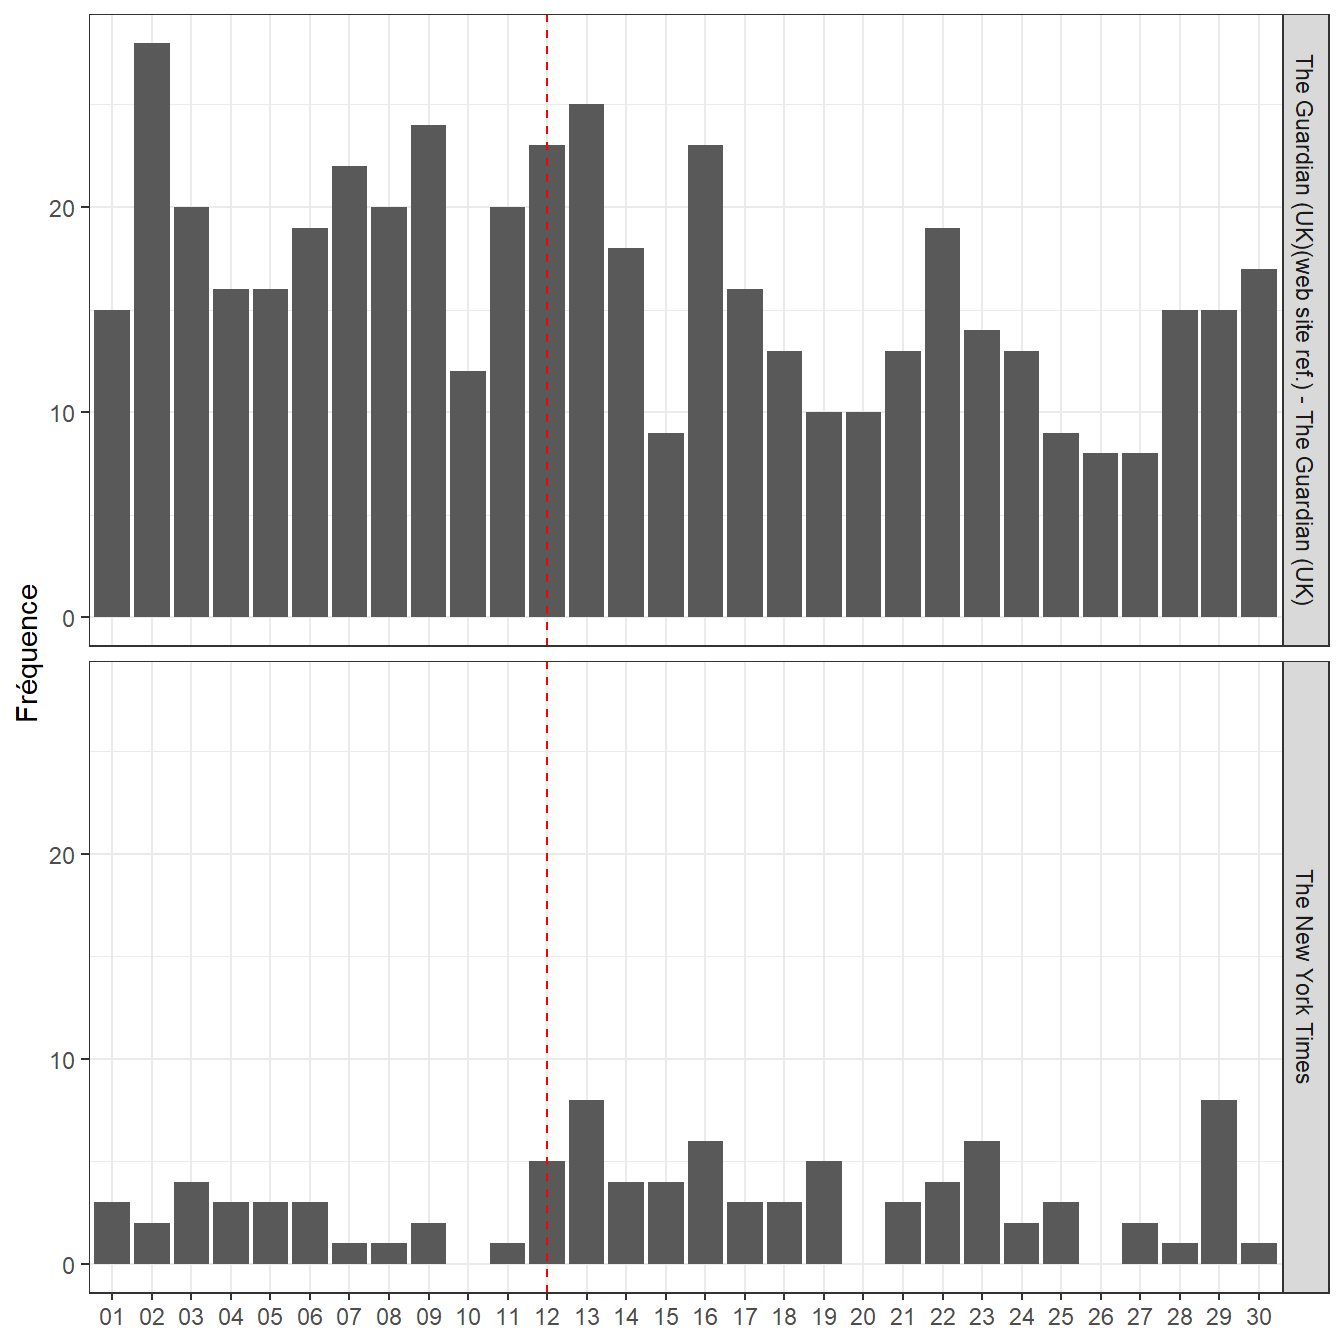
\includegraphics[width=0.8\linewidth]{bookdown-demo_files/figure-latex/201-1} 

}

\end{figure}

\begin{Shaded}
\begin{Highlighting}[]
\CommentTok{# screen_topics()}
\end{Highlighting}
\end{Shaded}

\texttt{revtools} n'est pas fait que pour importer des données au format bibliographique .ris, ou au format .bib, et de les transformer un tableau observations - variables ( bref, un dateframe). Il a des fonctions de visualisations rapides fort efficace. La plus spectaculaire est un outil de visualisation qui s'appuie sur deux modèles de détections de topics (ce sujet sera l'objet du chapitre 8), paramétrables de manière interactive en quelques minutes, et conçu avec \texttt{shiny}, le package star des graphes interactifs.

C'est un super outils pour avoir un premier coup d'oeil sur les données, un plug in super pratique.

On l'applique sur nos données. L'allure de l'interface est la suivante.

\begin{figure}
\centering
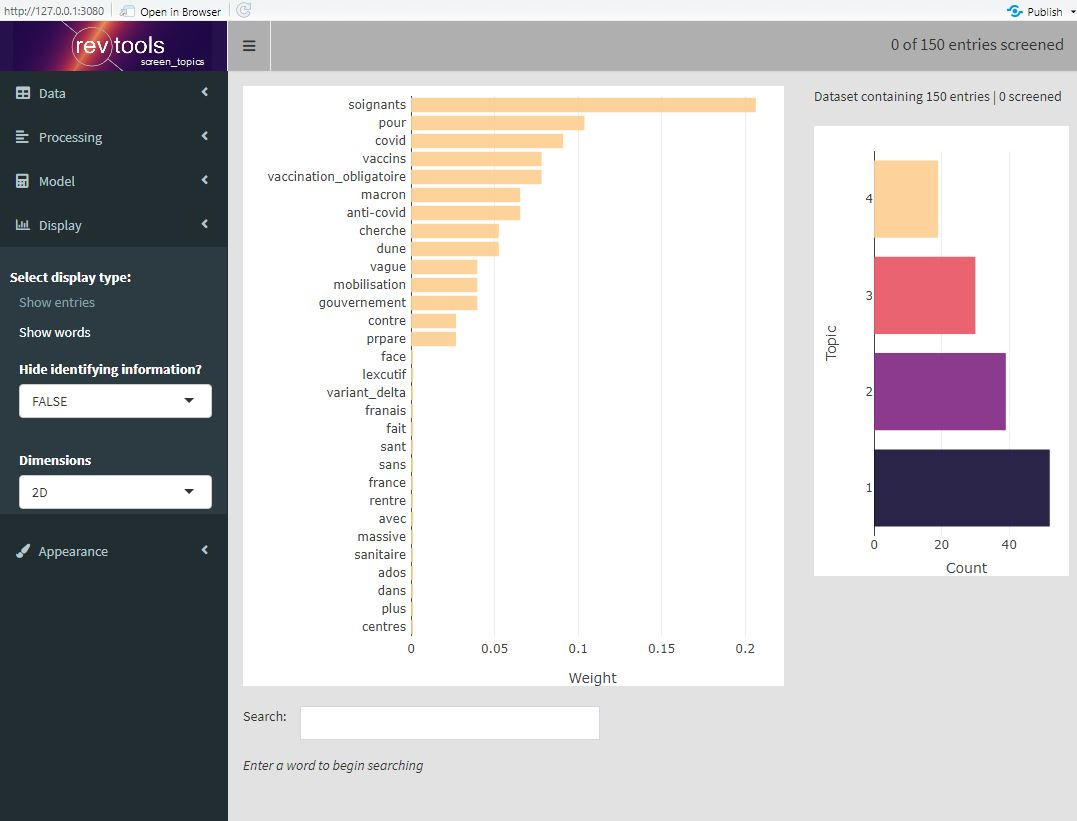
\includegraphics{./images/LDA_revtools.jpg}
\caption{screen\_topic}
\end{figure}

L'interface n'étant pas programmatique, on exporte quelques images en jpeg (un bouton dans l'interface permet de faire celà sans effort) et on les récupère avec \texttt{cowplot}, le package qui permet d'assembler des graphes et que nous utiliserons systématiquement dans ce cours.

\begin{Shaded}
\begin{Highlighting}[]
\NormalTok{p1 <-}\StringTok{ }\KeywordTok{ggdraw}\NormalTok{() }\OperatorTok{+}\StringTok{ }\KeywordTok{draw_image}\NormalTok{(}\StringTok{"./images/topic_espace.png"}\NormalTok{)}
\NormalTok{p2 <-}\StringTok{ }\KeywordTok{ggdraw}\NormalTok{() }\OperatorTok{+}\StringTok{ }\KeywordTok{draw_image}\NormalTok{(}\StringTok{"./images/topic_topic.png"}\NormalTok{)}
\NormalTok{p3 <-}\StringTok{ }\KeywordTok{ggdraw}\NormalTok{() }\OperatorTok{+}\StringTok{ }\KeywordTok{draw_image}\NormalTok{(}\StringTok{"./images/topic1.png"}\NormalTok{)}
\NormalTok{p4 <-}\StringTok{ }\KeywordTok{ggdraw}\NormalTok{() }\OperatorTok{+}\StringTok{ }\KeywordTok{draw_image}\NormalTok{(}\StringTok{"./images/topic5.png"}\NormalTok{)}

\KeywordTok{plot_grid}\NormalTok{(p1, p2 , }\DataTypeTok{ncol=}\DecValTok{2}\NormalTok{)}
\end{Highlighting}
\end{Shaded}

\begin{figure}

{\centering 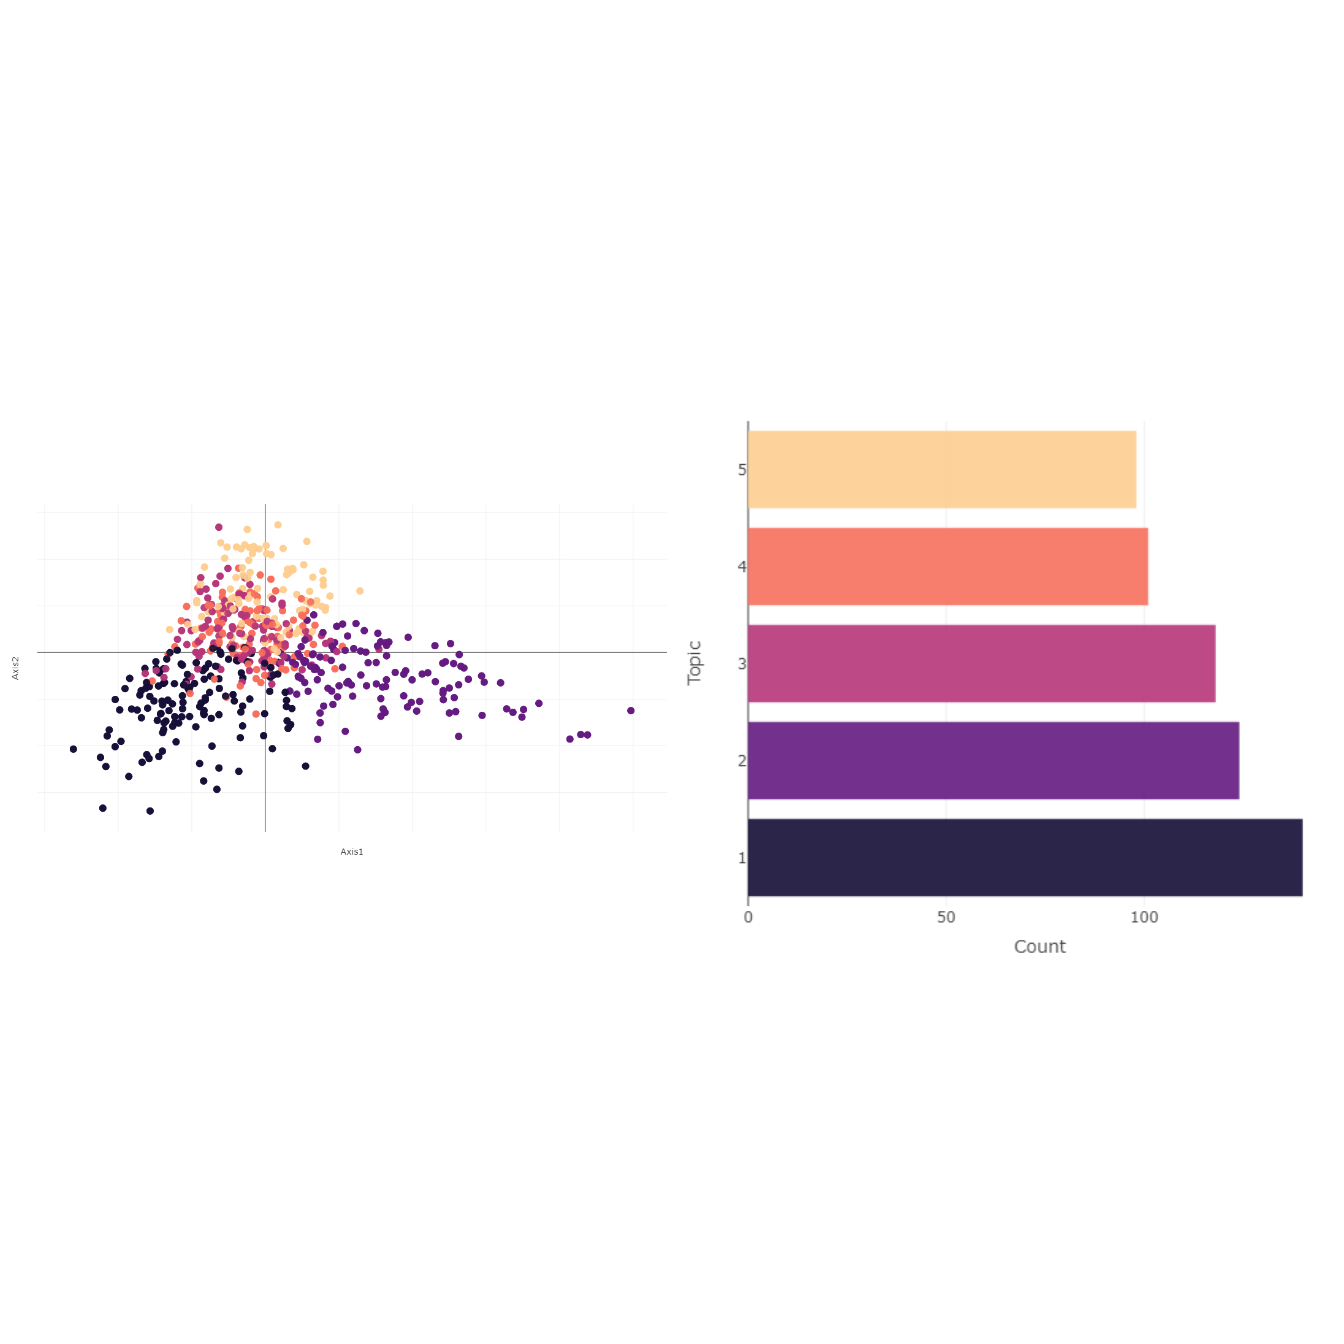
\includegraphics[width=0.8\linewidth]{bookdown-demo_files/figure-latex/202-1} 

}

\end{figure}

Et pour illustrer les graphiques des termes les plus proches du topic 1 et du topic 5. L'un est relatif à l'actualité austrlienne, l'autre à l'actualité anglaise.

\begin{Shaded}
\begin{Highlighting}[]
\KeywordTok{plot_grid}\NormalTok{(p3, p4 , }\DataTypeTok{ncol=}\DecValTok{1}\NormalTok{)}
\end{Highlighting}
\end{Shaded}

\begin{figure}

{\centering 
\includegraphics[width=0.8\linewidth]{bookdown-demo_files/figure-latex/203-1} 

}

\end{figure}

La méthode est sympa, rapide, sur le pouce, mais pas suffisante pour aller audelà et noatmment comparer les lignes éditoriales des deux titres que nous avons choisis. A ce stade de l'analyse c'est déjà beaucoup.

\hypertarget{jouer-avec-les-bases-bibliographiques}{%
\section{Jouer avec les bases bibliographiques}\label{jouer-avec-les-bases-bibliographiques}}

Fulltext

\url{https://books.ropensci.org/fulltext/data-sources.html}

\hypertarget{scrapping}{%
\section{Scrapping}\label{scrapping}}

Le scrapping correspond à un internet sauvage où la collecte d'information se traduit par une technique de chasseurs-cueilleurs, le glanage. c'est l'activité qui consiste à moissonner les informations disponibles sur le net en simulant et en automatisant la lecture par un navigateur ( on préfère l'expression des quebecois : des butinuers).

Elle consiste à construire un robot capable de lire et d'enregistrer les informations disponibles sous forme html puis à les distribuer (parsing) dans des tableaux structurés, selon une stratégie d'exploration du web préalablement définie. En réalité le scrapping pose deux problèmes :

\begin{itemize}
\tightlist
\item
  celui de la structure de recherche. C'est le problème que relève les spiders, des robots qui recherchent dans les pages des liens, et vont de proche en proche, de lien en lien, pour explorer un domaine.Ils peuvent être plus systématique et prendre avantage de l'organisation d'un site web pour enummérer les pages.
\item
  celui de la collecte de l'information sur chacune des pages. Il s'appuie sur le principe que le langage html est un langage à balise où le contenu et le contenant sont clairement séparés. Par exemple, dans le corps de texte d'une page on définira un titre par la balise

  dont l'instruction s'achève par la balise

  . On sépare ainsi clairement le contenu de la forme.
\end{itemize}

`

Un titre de niveau 1 (un gros titre)

\begin{verbatim}
<p>Un paragraphe.</p>

<h2>Un titre de niveau 2 (un sous titre)</h2>
  <p>Un paragraphe.</p>

  <h3>Un titre de niveau 3 (un sous-sous titre)</h3>
    <p>Etc.</p>
\end{verbatim}

`

Ultérieurement on pourra définirs les propriété graphiques d'une balise par des CSS. par exemple avec ceci les paragraphes seront publiés en caractère bleu.

\texttt{p\{\ \ \ \ \ color:\ blue;\ \}}

Ce qui nous intéresse n'est pas la décoration, mais le fait que les développeurs définissent des balises spécifiques pour chacun des éléments de leurs page web, et que si nous savons les repérer , nous avons le moyen de mieux lire le texte. Les balises sont la cible du scrapping

\hypertarget{rvest-avec-r}{%
\subsection{rvest avec r}\label{rvest-avec-r}}

De nombreuses ressources sont disponibles, mais pour en rester à r , le package rvest permet de réaliser des extractions simples mais suffisantes pour de nombreux usages.

une application rvest

\url{https://www.r-bloggers.com/2018/10/first-release-and-update-dates-of-r-packages-statistics/}

le package rvest est générique

\url{https://community.rstudio.com/t/scraping-messages-in-forum-using-rvest/27846/2}

\begin{Shaded}
\begin{Highlighting}[]
\KeywordTok{library}\NormalTok{(rvest)}

\CommentTok{# Scrape thread titles, thread links, authors and number of views}

\NormalTok{start <-}\StringTok{ "https://uberzone.fr/threads/si-la-vaccination-devient-obligatoire-vous-feriez-vous-vacciner-ou-changeriez-vous-de-corps-de-metier.17425"}

\NormalTok{x<-}\KeywordTok{c}\NormalTok{(}\StringTok{"/page-2"}\NormalTok{, }\StringTok{"/page-3"}\NormalTok{, }\StringTok{"/page-4"}\NormalTok{)}

\ControlFlowTok{for}\NormalTok{ (val }\ControlFlowTok{in}\NormalTok{ x)\{}
\NormalTok{  url<-}\KeywordTok{paste0}\NormalTok{(start,val)}
\NormalTok{  h <-}\StringTok{ }\KeywordTok{read_html}\NormalTok{(url)}

\NormalTok{post <-}\StringTok{ }\NormalTok{h }\OperatorTok
\StringTok{  }\KeywordTok{html_nodes}\NormalTok{(}\StringTok{".bbWrapper"}\NormalTok{) }\OperatorTok
\StringTok{  }\KeywordTok{html_text}\NormalTok{()}\OperatorTok
\StringTok{      }\KeywordTok{str_replace_all}\NormalTok{(}\DataTypeTok{pattern =} \StringTok{"}\CharTok{\textbackslash{}t}\StringTok{|}\CharTok{\textbackslash{}r}\StringTok{|}\CharTok{\textbackslash{}n}\StringTok{"}\NormalTok{, }\DataTypeTok{replacement =} \StringTok{""}\NormalTok{)}
\NormalTok{post}
\CommentTok{#authors <- h %>%}
\CommentTok{#  html_nodes(".username--style2 ") %>%}
\CommentTok{#  html_text() %>%}
\CommentTok{#  str_replace_all(pattern = "\textbackslash{}t|\textbackslash{}r|\textbackslash{}n", replacement = "")}

\CommentTok{# Create master dataset (and scrape messages in each thread in process)}

\NormalTok{master_data <-}\StringTok{ }
\StringTok{  }\KeywordTok{tibble}\NormalTok{(post)}
\NormalTok{rds_name<-}\KeywordTok{paste0}\NormalTok{(}\StringTok{"./data/df_"}\NormalTok{,}\KeywordTok{substr}\NormalTok{(val,}\DecValTok{2}\NormalTok{,}\DecValTok{6}\NormalTok{),}\StringTok{".rds"}\NormalTok{)}
\KeywordTok{saveRDS}\NormalTok{(master_data,rds_name)}
\NormalTok{\}}

\KeywordTok{head}\NormalTok{(master_data)}
\end{Highlighting}
\end{Shaded}

\begin{verbatim}
## # A tibble: 6 x 1
##   post                                                                          
##   <chr>                                                                         
## 1 "Je comprends pas pourquoi persistez-vous à vouloir convaincre alors que vous~
## 2 "Shibani a dit:Je comprends pas pourquoi persistez-vous à vouloir convaincre ~
## 3 "*****\"Celui qui ne pète pas et ne rote pas explose\"*****"                  
## 4 "mez a dit:Ta cirrhose et ton  Cancer du poumon (je te les souhaite pas faut ~
## 5 "Shibani a dit:Et puis sache que comme je l’ai déjà dit tu peux acheter ton p~
## 6 "*****\"Celui qui ne pète pas et ne rote pas explose\"*****"
\end{verbatim}

\hypertarget{des-probluxe8mes-pratiques-juridiques-et-uxe9thiques}{%
\subsection{Des problèmes pratiques, juridiques et éthiques}\label{des-probluxe8mes-pratiques-juridiques-et-uxe9thiques}}

La pratique du scrapping se heurte d'abord à une question technique. ce n'est pas un excercice facile, et il doit être confier à des spécialistes. Il se heurte aussi à différents problèmes d'ordre éthique et juridique. Si la pratique n'est pas interdite en tant que telle, elle se confronte à différents droits et principes éthiques

En termes pratiques, le scrapping crée des risques pour les sites :

\begin{itemize}
\tightlist
\item
  Le risque de deny of service, c'est à dire de saturer ou de parasiter un système et de s'exposer à ses contre-mesures.
\item
  Il contribue à la complexification du web, et implique une consommation excessive de ressources energétiques.
\end{itemize}

Et des risques pour la qualité dU recueil de données

\begin{itemize}
\tightlist
\item
  Le risque d'information parcellaires, tronquées, inexactes qui résultent de ces contre-mesures. Les producteurs développent des stratégies moins naives. L'exemple des pages numérotée par ordre de production auxquels on substitue un nombre au hasard pour annihilier l'information temporelle.
\item
  le risque matériel de mal lire les informations, pour des raison d'encodage approximatifs.
\end{itemize}

En termes de droits même les conditions légales relèvent de différents droits :

\begin{itemize}
\tightlist
\item
  De la propriété intellectuelle,
\item
  Du respect de la vie privée,
\item
  Du droit de la concurrence qui sans l'interdire, condamne la copie laissant espérer qu'une transformation des données fasse qu'il y échappeR.
\end{itemize}

Cependant des facilités et tolérances sont souvent accordées quand c'est dans un objectif de recherche et que des précautions minimales d'anonymisation ou de pseudonymisation sont prises, et que les règles de conservation et de destruction des données sont précisées.

En termes éthiques

\begin{itemize}
\tightlist
\item
  Un principe éthique essentiel dans la recherche, et ailleurs, et de ne pas nuire à la soci2té dans son ensemble, hors cette technique participe à la ``robotisation'' du web (plus de 50\% du trafic résulterait de la circulation des spi.ders , scrapers, sniffers et autres bots, comme dans la forêt une éthique écologique revient à préveler le minimal nécessaire pour l'étude entreprise
\end{itemize}

\hypertarget{les-api}{%
\section{les API}\label{les-api}}

Les API doivent être considérées comme la voie normale d'accès à l'information, du moins en droit. Elles relèvent du contrat. Le recours aux APIs est civilisé, ne serait-ce parce qu'on introduit une sorte d'étiquette, des règles de courtoisie, un système de reconnaissance réciproque et d'attribution de droits.

Sur le plan méthodologique elles présentent d'avantage de donner aux requêtes un caractère reproductible , mêmes si les bases visées peuvent varier. Elles asurent une grande fiabilité des données.

L'utilisation d'API lève l'ambiguïté légale qui accompagne le scraping et peut ainsi paraître comme plus ``civilisée''. Elle nécessite naturellement que le gestionnaire de la base de données fournisse les moyens de s'identifier et de requêter, elle peut avoir l'inconvénient d'être coûteuse quand l'accès est payant, ce qui sera de plus en plus le cas.

\hypertarget{un-tour-dhorizon-des-api}{%
\subsection{Un tour d'horizon des API}\label{un-tour-dhorizon-des-api}}

La plus part des grandes plateformes offrent des API plus ou moins ouvertes, examinons-en quelques une pour comprendre plus clairement leur intérêt méthodologique. On va se concentrer sur trois exemples : le firehose de tweeter, l'api de google maps, la Crunchbase.

Twitter n'est pas qu'un réseau social, c'est une gigantesque base de données qui enregistre les engagements et les humeurs de 500 millions d'humains à travers la planète et les centres d'intérêt. Elle permet potentiellement de saisir les opinions à différentes échelles géeographique et temporelle, y compris les plus locales et les plus courtes. Elle a le défaut de souffrir fortement de biais de sélection, le premier étant le biais d'engagement. Les passionnés d'un sujets parlent plus que les autres, une parôle mieux contrôlée.

Le cas de Google maps est passionnant à plus d'un égard. le premier d'entre eux est que dans l'effort d'indicer chaque objet de la planête, la base de données devient un référentiel universel, plus qu'une représentation intéressée du monde. Quand l'utilisateur communs cherche un chemin optimal, l'analyste de donnée trouve un socle pour ordonner le monde.

La Crunchbase construite par le média Techcrunch repertorie les créations de start-up et les levées de fonds qu'elles ont obtenues. Elle recence les dirigeants, les acquisitions, décrit les business model.

intégrité des bases de données, universalité des élément, interopérabilité, disponibilité

Les problèmes posés :

\begin{itemize}
\tightlist
\item
  justesse , précision et représentativité. leur constitution n'est pas aléatoire, leurs couverture reste partielle.
\item
  accessibilité, la privatisation du commun. Si pour le chercheur les APIS sont sur un plan de principe une merveille sur un plan plus social elle instaure des inégalités d'accès énormes aux données qui permettent de valoriser la connaissance. Ce mécanisme opère via deux canaux. Le premier est celui de la tarification qui ségrège les chercheurs en fonctions des ressources dont ils disposent. Le second passe par la couverture du champs, les données les plus précises et les plus denses se trouvent dans les régions les plus riches.
\item
  des catégorisations peu délibérées
\end{itemize}

\hypertarget{un-point-de-vue-plus-technique}{%
\subsection{un point de vue plus technique}\label{un-point-de-vue-plus-technique}}

\url{https://www.dataquest.io/blog/r-api-tutorial/}

\hypertarget{un-exemple-avec-rtweet}{%
\subsection{Un exemple avec Rtweet}\label{un-exemple-avec-rtweet}}

\url{https://cran.r-project.org/web/packages/rtweet/vignettes/intro.html}

Plusieurs packages de r permettent d'interroger le firehose ( la bouche d'incendie!) de twitter.

\url{https://www.rdocumentation.org/packages/rtweet/versions/0.7.0}

L'authentification ne nécesssite par de clé API, il suffit d'avoir son compte twitter ouvert. Cependant la fonction lookup\_coords requiert d'avoir une clé d'api ou google cloud map. Elle permet de selectionner sur un critère géographique.

\url{https://developer.twitter.com/en/docs/tutorials/getting-started-with-r-and-v2-of-the-twitter-api}

\begin{Shaded}
\begin{Highlighting}[]
\CommentTok{#une boucle pour multiplier les hashtag }

\NormalTok{x<-}\KeywordTok{c}\NormalTok{(}\StringTok{"#getaround"}\NormalTok{,}\StringTok{"#Uber"}\NormalTok{, }\StringTok{"#heetch"}\NormalTok{)}

\ControlFlowTok{for}\NormalTok{ (val }\ControlFlowTok{in}\NormalTok{ x) \{}
\NormalTok{  tweets <-}\StringTok{ }\KeywordTok{search_tweets}\NormalTok{(val,}\DataTypeTok{n=}\DecValTok{20000}\NormalTok{,}\DataTypeTok{retryonratelimit =} \OtherTok{TRUE}\NormalTok{)}\OperatorTok\StringTok{ }\CommentTok{#geocode = lookup_coords("france")}
\StringTok{      }\KeywordTok{mutate}\NormalTok{(}\DataTypeTok{search=}\NormalTok{val)}
  \KeywordTok{write_rds}\NormalTok{(tweets,}\KeywordTok{paste0}\NormalTok{(}\StringTok{"tweets_"}\NormalTok{,}\KeywordTok{substring}\NormalTok{(val,}\DecValTok{2}\NormalTok{),}\StringTok{".rds"}\NormalTok{))}
\NormalTok{\}}

\NormalTok{df_blablacar<-}\KeywordTok{readRDS}\NormalTok{(}\StringTok{"./data/tweets_blablacar.rds"}\NormalTok{)}
\NormalTok{df_uber<-}\KeywordTok{readRDS}\NormalTok{(}\StringTok{"./data/tweets_uber.rds"}\NormalTok{)}
\NormalTok{df_heetch<-}\KeywordTok{readRDS}\NormalTok{(}\StringTok{"./data/tweets_heetch.rds"}\NormalTok{)}

\NormalTok{df<-}\KeywordTok{rbind}\NormalTok{(df_blablacar,df_uber )}

\KeywordTok{ls}\NormalTok{(df_blablacar)}

\NormalTok{foo<-df }\OperatorTok\StringTok{ }\KeywordTok{select}\NormalTok{(account_lang, geo_coords,country_code, country, account_lang,place_name)}
\end{Highlighting}
\end{Shaded}

On laisse le lecteur explorer les différentes fonctionnalités du package. On aime cependant celle-ci qui sample le flux courrant au taux annoncé de 1\%. Voici l'extraction de ce qui se dit en france pendant 10 mn (600s). La procédure peut donner une sorte de benchmark auquel on peut comparer une recherche plus spécifique.

\begin{Shaded}
\begin{Highlighting}[]
\NormalTok{rt <-}\StringTok{ }\KeywordTok{stream_tweets}\NormalTok{(}\KeywordTok{lookup_coords}\NormalTok{(}\StringTok{"france"}\NormalTok{), }\DataTypeTok{timeout =} \DecValTok{600}\NormalTok{)}
\end{Highlighting}
\end{Shaded}

\hypertarget{la-gestion-des-documents}{%
\section{La gestion des documents}\label{la-gestion-des-documents}}

voir aussi

\url{https://cran.r-project.org/web/packages/fulltext/fulltext.pdf}

\hypertarget{extraire-du-texte-des-pdf}{%
\subsection{Extraire du texte des pdf}\label{extraire-du-texte-des-pdf}}

Le package \href{https://ropensci.org/blog/2016/03/01/pdftools-and-jeroen/}{pdftools} est parfaitement adapté à la tâche. Des fonctions simples extraient différents éléments du pdf :
* les information relative au document pdf lui-même
* La liste des polices employées
* Les attachements
* La table des matières ( si elle a été encodée)
* et naturellement le texte dans un ordre de droite à gauche et de ligne à ligne, reconnaissant cependant les retrour chariot, et sauts de lignes.

Chaque page est contenue dans une ligne.

\begin{Shaded}
\begin{Highlighting}[]
\KeywordTok{library}\NormalTok{(pdftools)}

\NormalTok{info <-}\StringTok{ }\KeywordTok{pdf_info}\NormalTok{(}\StringTok{"./pdf/2021neoliberalismegouverner_Meunier_Esprit.pdf"}\NormalTok{)}
\NormalTok{info}
\end{Highlighting}
\end{Shaded}

\begin{verbatim}
## $version
## [1] "1.4"
## 
## $pages
## [1] 12
## 
## $encrypted
## [1] FALSE
## 
## $linearized
## [1] TRUE
## 
## $keys
## $keys$Author
## [1] ""
## 
## $keys$Creator
## [1] ""
## 
## $keys$Keywords
## [1] ""
## 
## $keys$Producer
## [1] "TCPDF 6.2.12 (http://www.tcpdf.org)"
## 
## $keys$Subject
## [1] ""
## 
## $keys$Title
## [1] "Le néolibéralisme et l\220art de gouverner"     
## 
## $keys$Trapped
## [1] ""
## 
## 
## $created
## [1] "2021-05-04 17:33:26 CEST"
## 
## $modified
## [1] "2021-07-02 14:10:59 CEST"
## 
## $metadata
## [1] "<?xpacket begin=\"\" id=\"W5M0MpCehiHzreSzNTczkc9d\"?>\n<x:xmpmeta xmlns:x=\"adobe:ns:meta/\" x:xmptk=\"Adobe XMP Core 5.6-c017 91.164464, 2020/06/15-10:20:05        \">\n   <rdf:RDF xmlns:rdf=\"http://www.w3.org/1999/02/22-rdf-syntax-ns#\">\n      <rdf:Description rdf:about=\"\"\n            xmlns:dc=\"http://purl.org/dc/elements/1.1/\"\n            xmlns:xmp=\"http://ns.adobe.com/xap/1.0/\"\n            xmlns:pdf=\"http://ns.adobe.com/pdf/1.3/\"\n            xmlns:xmpMM=\"http://ns.adobe.com/xap/1.0/mm/\"\n            xmlns:pdfaExtension=\"http://www.aiim.org/pdfa/ns/extension/\"\n            xmlns:pdfaSchema=\"http://www.aiim.org/pdfa/ns/schema#\"\n            xmlns:pdfaProperty=\"http://www.aiim.org/pdfa/ns/property#\">\n         <dc:format>application/pdf</dc:format>\n         <dc:title>\n            <rdf:Alt>\n               <rdf:li xml:lang=\"x-default\">Le néolibéralisme et lâ<U+0080><U+0099>art de gouverner</rdf:li>\n            </rdf:Alt>\n         </dc:title>\n         <dc:creator>\n            <rdf:Seq>\n               <rdf:li/>\n            </rdf:Seq>\n         </dc:creator>\n         <dc:description>\n            <rdf:Alt>\n               <rdf:li xml:lang=\"x-default\"/>\n            </rdf:Alt>\n         </dc:description>\n         <dc:subject>\n            <rdf:Bag>\n               <rdf:li/>\n            </rdf:Bag>\n         </dc:subject>\n         <xmp:CreateDate>2021-05-04T17:33:26+02:00</xmp:CreateDate>\n         <xmp:CreatorTool/>\n         <xmp:ModifyDate>2021-07-02T14:10:59+02:00</xmp:ModifyDate>\n         <xmp:MetadataDate>2021-07-02T14:10:59+02:00</xmp:MetadataDate>\n         <pdf:Keywords/>\n         <pdf:Producer>TCPDF 6.2.12 (http://www.tcpdf.org)</pdf:Producer>\n         <xmpMM:DocumentID>uuid:95265141-0cc7-e3b8-5dff-27561dd19960</xmpMM:DocumentID>\n         <xmpMM:InstanceID>uuid:71358868-c7aa-4ef5-8b30-f18fa6312a88</xmpMM:InstanceID>\n         <pdfaExtension:schemas>\n            <rdf:Bag>\n               <rdf:li rdf:parseType=\"Resource\">\n                  <pdfaSchema:namespaceURI>http://ns.adobe.com/pdf/1.3/</pdfaSchema:namespaceURI>\n                  <pdfaSchema:prefix>pdf</pdfaSchema:prefix>\n                  <pdfaSchema:schema>Adobe PDF Schema</pdfaSchema:schema>\n               </rdf:li>\n               <rdf:li rdf:parseType=\"Resource\">\n                  <pdfaSchema:namespaceURI>http://ns.adobe.com/xap/1.0/mm/</pdfaSchema:namespaceURI>\n                  <pdfaSchema:prefix>xmpMM</pdfaSchema:prefix>\n                  <pdfaSchema:schema>XMP Media Management Schema</pdfaSchema:schema>\n                  <pdfaSchema:property>\n                     <rdf:Seq>\n                        <rdf:li rdf:parseType=\"Resource\">\n                           <pdfaProperty:category>internal</pdfaProperty:category>\n                           <pdfaProperty:description>UUID based identifier for specific incarnation of a document</pdfaProperty:description>\n                           <pdfaProperty:name>InstanceID</pdfaProperty:name>\n                           <pdfaProperty:valueType>URI</pdfaProperty:valueType>\n                        </rdf:li>\n                     </rdf:Seq>\n                  </pdfaSchema:property>\n               </rdf:li>\n               <rdf:li rdf:parseType=\"Resource\">\n                  <pdfaSchema:namespaceURI>http://www.aiim.org/pdfa/ns/id/</pdfaSchema:namespaceURI>\n                  <pdfaSchema:prefix>pdfaid</pdfaSchema:prefix>\n                  <pdfaSchema:schema>PDF/A ID Schema</pdfaSchema:schema>\n                  <pdfaSchema:property>\n                     <rdf:Seq>\n                        <rdf:li rdf:parseType=\"Resource\">\n                           <pdfaProperty:category>internal</pdfaProperty:category>\n                           <pdfaProperty:description>Part of PDF/A standard</pdfaProperty:description>\n                           <pdfaProperty:name>part</pdfaProperty:name>\n                           <pdfaProperty:valueType>Integer</pdfaProperty:valueType>\n                        </rdf:li>\n                        <rdf:li rdf:parseType=\"Resource\">\n                           <pdfaProperty:category>internal</pdfaProperty:category>\n                           <pdfaProperty:description>Amendment of PDF/A standard</pdfaProperty:description>\n                           <pdfaProperty:name>amd</pdfaProperty:name>\n                           <pdfaProperty:valueType>Text</pdfaProperty:valueType>\n                        </rdf:li>\n                        <rdf:li rdf:parseType=\"Resource\">\n                           <pdfaProperty:category>internal</pdfaProperty:category>\n                           <pdfaProperty:description>Conformance level of PDF/A standard</pdfaProperty:description>\n                           <pdfaProperty:name>conformance</pdfaProperty:name>\n                           <pdfaProperty:valueType>Text</pdfaProperty:valueType>\n                        </rdf:li>\n                     </rdf:Seq>\n                  </pdfaSchema:property>\n               </rdf:li>\n            </rdf:Bag>\n         </pdfaExtension:schemas>\n      </rdf:Description>\n   </rdf:RDF>\n</x:xmpmeta>\n                                                                                                    \n                                                                                                    \n                                                                                                    \n                                                                                                    \n                                                                                                    \n                                                                                                    \n                                                                                                    \n                                                                                                    \n                                                                                                    \n                                                                                                    \n                                                                                                    \n                                                                                                    \n                                                                                                    \n                                                                                                    \n                                                                                                    \n                                                                                                    \n                                                                                                    \n                                                                                                    \n                                                                                                    \n                                                                                                    \n                           \n<?xpacket end=\"w\"?>"
## 
## $locked
## [1] FALSE
## 
## $attachments
## [1] FALSE
## 
## $layout
## [1] "single_page"
\end{verbatim}

\begin{Shaded}
\begin{Highlighting}[]
\NormalTok{fonts <-}\StringTok{ }\KeywordTok{pdf_fonts}\NormalTok{(}\StringTok{"./pdf/2021neoliberalismegouverner_Meunier_Esprit.pdf"}\NormalTok{)}

\NormalTok{files <-}\StringTok{ }\KeywordTok{pdf_attachments}\NormalTok{(}\StringTok{"./pdf/2021neoliberalismegouverner_Meunier_Esprit.pdf"}\NormalTok{)}

\NormalTok{toc <-}\StringTok{ }\KeywordTok{pdf_toc}\NormalTok{(}\StringTok{"./pdf/2021neoliberalismegouverner_Meunier_Esprit.pdf"}\NormalTok{) }\CommentTok{#il n'y a pas de table des matière dans ce texte}

\NormalTok{text <-}\StringTok{ }\KeywordTok{pdf_text}\NormalTok{(}\StringTok{"./pdf/2021neoliberalismegouverner_Meunier_Esprit.pdf"}\NormalTok{)}
\KeywordTok{cat}\NormalTok{(text[[}\DecValTok{1}\NormalTok{]]) }\CommentTok{# pour afficher le texte de la page 1}
\end{Highlighting}
\end{Shaded}

\begin{verbatim}
## Le néolibéralisme
## et l’art de gouverner
## À propos de Naissance de la biopolitique
## de Michel Foucault
## François Meunier
## 
## 
## 
## 
## O          n dit parfois du métier de l’historien qu’il consiste avant tout
##            à découper en périodes, à indiquer les ruptures dans le temps
##            historique, à montrer les changements d’environnement et
## de paradigme. C’est à ce travail que se consacre Michel Foucault dans
## son célèbre cours de 1978-1979 au Collège de France connu sous le
## nom de Naissance de la biopolitique 1. Il devait porter initialement sur la
## « biopolitique », un mot chatoyant recouvrant les pratiques politiques
## contemporaines autour du vivant (santé, démographie, sexualité, etc.).
## Mais Foucault voulait montrer d’abord à quel point la venue du libé-
## ralisme avait modifié en profondeur les pratiques gouvernementales.
## Première rupture, celle advenue à la fin du xviiie siècle avec le libéralisme
## économique classique, selon lequel le marché devient l’instance clé dans
## l’art de gouverner, donnant à l’action publique un lieu de légitimation en
## même temps que des limites. Seconde rupture, celle qui sépare libéralisme
## et néolibéralisme, que Foucault situe dans l’après-guerre en Allemagne,
## avec ce qu’on appelle « l’ordolibéralisme ».
## 
## 
## Équivocité du néolibéralisme
## Reprenant, quelque quarante ans après, le fil de ce cours, nous remettons
## ici en cause le découpage historique. D’abord, il nous semble que ce
## 
## 1 - Michel Foucault, Naissance de la biopolitique. Cours au Collège de France (1978-1979), Paris,
## EHESS/Seuil/Gallimard, 2004.
## 
## 
## 
## 
## · ESPRIT · Mai 2021                                                                                 83/
\end{verbatim}

Il va falloir traiter ce texte en analysant précisément sa composition. Et en définissant une séquence d'opérations logiques qui permette un premier nettoyage du texte. Dans l'exemple on va de plus essayer de respecter la structure en paragraphe du texte.

\begin{itemize}
\tightlist
\item
  Suprimer haut et bas de pages
\item
  Supprimer les sauts de ligne
\item
  Identifier les sauts de paragraphe
\item
  Enlever les notes de bas de page
\item
  Corriger l'hyphénation ()
\item
  regrouper les document en un seul bloc de texte
\item
  le splitter en autant de paragraphes.
\end{itemize}

On va utiliser des fonctions de traitement de chaines de caractère avec Stringret le recours à l'art ( ici simple) des regex auxquels on consacre un développement dans le chapitres X.

\begin{Shaded}
\begin{Highlighting}[]
\NormalTok{tex<-}\StringTok{ }\KeywordTok{as.data.frame}\NormalTok{(text)}
\NormalTok{tex[}\DecValTok{1}\NormalTok{,]}
\end{Highlighting}
\end{Shaded}

\begin{verbatim}
## [1] "Le néolibéralisme\net l’art de gouverner\nÀ propos de Naissance de la biopolitique\nde Michel Foucault\nFrançois Meunier\n\n\n\n\nO          n dit parfois du métier de l’historien qu’il consiste avant tout\n           à découper en périodes, à indiquer les ruptures dans le temps\n           historique, à montrer les changements d’environnement et\nde paradigme. C’est à ce travail que se consacre Michel Foucault dans\nson célèbre cours de 1978-1979 au Collège de France connu sous le\nnom de Naissance de la biopolitique 1. Il devait porter initialement sur la\n« biopolitique », un mot chatoyant recouvrant les pratiques politiques\ncontemporaines autour du vivant (santé, démographie, sexualité, etc.).\nMais Foucault voulait montrer d’abord à quel point la venue du libé-\nralisme avait modifié en profondeur les pratiques gouvernementales.\nPremière rupture, celle advenue à la fin du xviiie siècle avec le libéralisme\néconomique classique, selon lequel le marché devient l’instance clé dans\nl’art de gouverner, donnant à l’action publique un lieu de légitimation en\nmême temps que des limites. Seconde rupture, celle qui sépare libéralisme\net néolibéralisme, que Foucault situe dans l’après-guerre en Allemagne,\navec ce qu’on appelle « l’ordolibéralisme ».\n\n\nÉquivocité du néolibéralisme\nReprenant, quelque quarante ans après, le fil de ce cours, nous remettons\nici en cause le découpage historique. D’abord, il nous semble que ce\n\n1 - Michel Foucault, Naissance de la biopolitique. Cours au Collège de France (1978-1979), Paris,\nEHESS/Seuil/Gallimard, 2004.\n\n\n\n\n· ESPRIT · Mai 2021                                                                                 83/\n"
\end{verbatim}

\begin{Shaded}
\begin{Highlighting}[]
\NormalTok{t_reg<-}\KeywordTok{str_replace}\NormalTok{(tex}\OperatorTok{$}\NormalTok{text,}\StringTok{"[}\CharTok{\textbackslash{}\textbackslash{}}\StringTok{s+].*Meunier[}\CharTok{\textbackslash{}n}\StringTok{]+"}\NormalTok{, }\StringTok{" "}\NormalTok{) }\CommentTok{# entete droite}
\CommentTok{## on selectionne tout bloc de texte qui commence par un nombre indéterminée de blanc qui s'achève par n'importe quel caractère répétés mais terimé par la séquence Meunier suivie de sauts de ligne.}
\NormalTok{t_reg<-}\KeywordTok{str_replace}\NormalTok{(t_reg,}\StringTok{"[}\CharTok{\textbackslash{}\textbackslash{}}\StringTok{s+].*gouverner[}\CharTok{\textbackslash{}n}\StringTok{]+"}\NormalTok{, }\StringTok{" "}\NormalTok{) }\CommentTok{# entete gauche}
\NormalTok{t_reg<-}\KeywordTok{str_replace_all}\NormalTok{(t_reg,}\StringTok{"[}\CharTok{\textbackslash{}\textbackslash{}}\StringTok{s+].*2021[}\CharTok{\textbackslash{}n}\StringTok{]"}\NormalTok{, }\StringTok{" "}\NormalTok{) }\CommentTok{# bas de page  gauche}
\NormalTok{t_reg<-}\KeywordTok{str_replace_all}\NormalTok{(t_reg,}\StringTok{"ESPRIT.*[}\CharTok{\textbackslash{}n}\StringTok{]"}\NormalTok{, }\StringTok{" "}\NormalTok{) }\CommentTok{# bas de page droit}

\CommentTok{#on marque les paragraphes avec la chaine XXX pour les splitter dans un second temps}


\NormalTok{t_reg<-}\KeywordTok{str_replace_all}\NormalTok{(t_reg,}\StringTok{"}\CharTok{\textbackslash{}n\textbackslash{}n\textbackslash{}n}\StringTok{"}\NormalTok{, }\StringTok{"XXX"}\NormalTok{) }

\CommentTok{# On supprime les saut de ligne en les remplaçant par un espace}

\NormalTok{t_reg<-}\KeywordTok{str_replace_all}\NormalTok{(t_reg,}\StringTok{"[}\CharTok{\textbackslash{}n}\StringTok{]"}\NormalTok{, }\StringTok{" "}\NormalTok{)}

\CommentTok{#on enlève les notes de bas de page}
\NormalTok{t_reg<-}\KeywordTok{str_replace_all}\NormalTok{(t_reg,}\StringTok{"}\CharTok{\textbackslash{}\textbackslash{}}\StringTok{d}\CharTok{\textbackslash{}\textbackslash{}}\StringTok{s[}\CharTok{\textbackslash{}\textbackslash{}}\StringTok{-].*XXX"}\NormalTok{, }\StringTok{"XXX"}\NormalTok{)}

\CommentTok{#on regroupe les pages}

\NormalTok{t<-}\KeywordTok{paste}\NormalTok{(}\KeywordTok{unlist}\NormalTok{(}\KeywordTok{t}\NormalTok{(t_reg)), }\DataTypeTok{collapse=}\StringTok{" "}\NormalTok{)}



\CommentTok{#on enlève les notes dans le texte}

\NormalTok{t<-}\KeywordTok{str_replace_all}\NormalTok{(t,}\StringTok{"[A-Z|a-z]+}\CharTok{\textbackslash{}\textbackslash{}}\StringTok{d}\CharTok{\textbackslash{}\textbackslash{}}\StringTok{s[}\CharTok{\textbackslash{}\textbackslash{}}\StringTok{-]"}\NormalTok{, }\StringTok{" "}\NormalTok{)}

\NormalTok{t<-}\KeywordTok{str_replace_all}\NormalTok{(t,}\StringTok{"}\CharTok{\textbackslash{}\textbackslash{}}\StringTok{d}\CharTok{\textbackslash{}\textbackslash{}}\StringTok{d}\CharTok{\textbackslash{}\textbackslash{}}\StringTok{s[}\CharTok{\textbackslash{}\textbackslash{}}\StringTok{-]"}\NormalTok{, }\StringTok{" "}\NormalTok{)}

\CommentTok{#hyphenation}

\NormalTok{t<-}\KeywordTok{str_replace_all}\NormalTok{(t,}\StringTok{"[A-Z|a-z]+[}\CharTok{\textbackslash{}\textbackslash{}}\StringTok{-]}\CharTok{\textbackslash{}\textbackslash{}}\StringTok{s"}\NormalTok{, }\StringTok{""}\NormalTok{)}

\CommentTok{#pour enlever les espaces excedentaires}

\NormalTok{t<-}\KeywordTok{str_squish}\NormalTok{(t)}
\NormalTok{t}
\end{Highlighting}
\end{Shaded}

\begin{verbatim}
## [1] "Le néolibéralisme À propos de Naissance de la biopolitique de Michel Foucault O n dit parfois du métier de l’historien qu’il consiste avant tout à découper en périodes, à indiquer les ruptures dans le temps historique, à montrer les changements d’environnement et de paradigme. C’est à ce travail que se consacre Michel Foucault dans son célèbre cours de 1978-1979 au Collège de France connu sous le nom de Naissance de la biopolitique 1. Il devait porter initialement sur la « biopolitique », un mot chatoyant recouvrant les pratiques politiques contemporaines autour du vivant (santé, démographie, sexualité, etc.). Mais Foucault voulait montrer d’abord à quel point la venue du libé- ralisme avait modifié en profondeur les pratiques gouvernementales. Première rupture, celle advenue à la fin du xviiie siècle avec le libéralisme économique classique, selon lequel le marché devient l’instance clé dans l’art de gouverner, donnant à l’action publique un lieu de légitimation en même temps que des limites. Seconde rupture, celle qui sépare libéralisme et néolibéralisme, que Foucault situe dans l’après-guerre en Allemagne, avec ce qu’on appelle « l’ordolibéralisme ».XXXÉquivocité du néolibéralisme Reprenant, quelque quarante ans après, le fil de ce cours, nous remettons ici en cause le découpage historique. D’abord, il nous semble que ce XXX · n’est pas autour de la notion de marché qu’il faut attacher la genèse du libéralisme classique, mais plutôt autour de l’idée d’une société capable de s’organiser en dehors du prince. Ensuite, la rupture constituante du néolibéralisme se situe postérieurement à l’arrivée de Reagan et Thatcher au pouvoir, lorsqu’on aura théorisé et mis en pratique la financiarisation de l’économie comme instance ordonnatrice (cela donc après le cours de Foucault). S’agissant de l’ordolibéralisme, il présente de fortes continuités avec le libéralisme classique, même s’il garde les marques d’un mer- cantilisme qui s’est développé tardivement en Allemagne. Il n’est guère étonnant que ce courant se soit fondu si aisément dans le modèle social de marché auquel on associe davantage la social-démocratie allemande que le libéralisme débridé. Cela devrait aider à mieux caractériser ce qu’il faut entendre par « néo- libéralisme », un mot devenu équivoque. Si l’on peut créditer Foucault d’être parmi ceux qui l’ont inventé, c’est plus chez lui par commodité verbale2. Lorsqu’il rédigea le résumé du cours au terme de son année, c’est significativement le seul mot de « libéralisme » qu’il a retenu. Le cours bénéficie toujours d’une forte aura. En effet, il est la seule incursion de Foucault dans l’histoire contemporaine ; il introduit le concept de gouvernementalité, qui a acquis une certaine place dans la science politique. Son style attire, mélange d’écrit et d’oral où la pensée se construit par bonds successifs et inattendus, avançant « en écrevisse » comme il le dit. Le texte déroute aussi parce qu’il ne cherche pas à construire un contre-modèle quand il analyse le courant intellectuel libéral. La dissection des textes s’accompagne à l’évidence chez lui d’une certaine fascination. Il rabroue même son public quand celui-ci voudrait le voir glisser vers des objections trop faciles au libéralisme3. Il n’est pas étonnant que des milieux se réclamant du libéralisme, y compris poli- tique, s’en réclament presque autant que ses adversaires.XXX XXX Enfin et surtout, le texte se concentre pour l’essentiel sur l’Allemagne, un pays que Foucault connaissait très bien pour y avoir enseigné : « Dans cette seconde moitié du xxe siècle, le libéralisme est un mot qui nous vient d’Allemagne. » C’est l’ordolibéralisme qu’il désigne comme « néolibéral ». Il traite assez peu, de façon surprenante, de ce qu’on appelle l’École de Chicago, que Foucault appelle l’anarcho-libéralisme, née dans les années 1930, dont l’influence a été majeure dans le renversement idéologique opéré à l’époque de Reagan aux États-Unis : « Je ne suis pas sûr d’avoir le temps de parler des Américains. »XXXL’âge classique L’économie politique, à partir de Turgot et Smith, s’est bâtie sur une critique du régime mercantiliste. Le mercantilisme, c’est l’idéologie d’un État en constitution, qui organise l’hégémonie du prince, qui pour cela capte des richesses, s’organise administrativement, privilégie la bonne collecte des impôts et l’exportation, et où un ordre juridique se substitue au droit divin du souverain. Cette critique avait commencé sur le plan des idées politiques. Chez Locke et Spinoza, le citoyen naissait et la liberté politique était réclamée. Mais on ne touchait pas encore à l’organisation sociale du royaume. Le pas en avant fait par l’économie politique a été de donner toute sa place à la nouvelle classe des marchands, consciente désormais de contribuer à l’enrichissement du royaume. On quittait une vision assez prédatrice, où l’échange était essentiellement un jeu à somme nulle, où ce que gagnait un pays était une perte pour l’autre et où le talent du prince consistait à ce que son pays se sorte bien de cette confrontation. La vision classique est inverse : il y a possibilité d’un échange équitable, qui se fait fina- lement au bénéfice – « à l’intérêt » – des deux parties4. Il y a possibilité d’une croissance endogène où le marchand réinvestit son profit dans des activités nouvelles, une morale que le puritain anglais avait parfaitement intériorisée. Il s’introduit à plein la notion de concurrence qui gomme les situations de rente. Naissait dans la foulée la notion d’intérêt général et de bien commun, davantage au centre des intérêts individuels dans la XXX · tradition britannique que l’expression d’une souveraineté première dans la tradition française. Foucault décrit cette transition mais force le trait quand il indique, dans une phrase significative, que cet âge classique est celui où le marché devient un principe de régulation politique en remplacement de l’ordre juridique qui prévalait auparavant. Selon lui, c’est désormais la légi- timité marchande qui non seulement limite mais organise et structure la décision publique. Elle devient le « lieu de véridiction » de l’action gou- vernementale : « Ce lieu de formation de la vérité […], il faut le laisser jouer avec le moins d’interventions possibles pour qu’il puisse et formuler sa vérité et la proposer comme règle et norme à la pratique gouvernementale. Ce lieu de vérité, c’est bien entendu non pas la tête des économistes, mais le marché 5. » Mais Foucault anticipe de près de deux siècles. D’une part, la prévalence du droit est plus manifeste encore à l’époque classique qu’à âge préclassique ; les structures de marché s’approfondissent et s’appuient sur des contrats établis, le mot étant d’ailleurs repris dans la notion de contrat social qui naît à cette période. D’autre part, il n’y a pas pour les classiques une rupture dans la conception du marché. Les prix auraient été avant cette période, dit Foucault, des prix ordonnés selon des critères d’équité ou de stabilité sociale, des prix « justes » et non, comme postérieurement, des prix régis par la loi de l’offre et la demande. C’est ce que dément une bonne part de l’historiographie moderne, à partir d’auteurs comme de Roover ou Todeschini6, pour qui le juste prix n’était rien d’autre que le prix de marché, mais d’un marché mis en position de bien fonctionner, une idée qui fera apparaître progressivement le concept de concurrence, très net chez les auteurs de la seconde scolastique dans l’Espagne de la fin du xvie siècle, celui de monopole étant déjà ancien. La rupture, majeure, avec le mercantilisme existe, mais elle est que la société peut se libérer du prince, que l’économie peut fonctionner malgré sa dispersion, sans coordination venue d’en haut. La fameuse « main invisible », dans le seul passage de La Richesse des nations où Smith la mentionne, y est comme une image pour résoudre ce paradoxe d’une XXX économie qui évite le chaos alors que les centres de décision (de pouvoir) sont dispersés, chacun d’eux ne prenant nullement en compte la décision des autres. Il s’agit là d’une notion commune qui exprime la différence entre la cause finale d’une action et l’intention des agents7. Sur ce point, nos économistes restent même en retrait du libéralisme politique d’un Locke ou d’un Montesquieu pour qui la société fonctionne non pas malgré sa dispersion mais grâce à une dispersion des pouvoirs et des centres de décision, qui devient l’élément régulateur par lequel on atteint le bien commun. Dans ce contexte, le gouvernement prend une place très différente. La société connaît des contraintes et interactions multiples et l’art de gou- verner consiste à les prendre en compte. Il s’introduit une rationalité différente, une rationalité des fins, que Foucault décrit très bien. La question posée est celle de l’utilité ou de l’efficacité des effets induits d’une mesure. Mais ce qui est important Ce qui est important et moins et moins bien vu par Foucault est que bien vu par Foucault est que cette rationalité nouvelle peut justifier cette rationalité nouvelle peut autant l’intervention publique que son justifier autant l’intervention retrait. On pourra soutenir dans un cas publique que son retrait. que l’autonomie de la société signifie que le gouvernement est en trop, qu’il perturbe l’ordre économique ou qu’il interfère de façon coercitive sur la liberté individuelle. Mais on peut alternativement affirmer que le gouvernement a en main des guides et préceptes, une rationalité économique, qui l’autorisent et qui même le poussent à intervenir dans l’ordre économique. On voit poindre ici une bifurcation profonde, toujours actuelle, qui verra tout à la fois un Hayek libertarien ou un Keynes interventionniste se réclamer de la tradition économique libérale. À vrai dire, pour ce second courant libéral, on peut corriger la phrase de Foucault citée plus haut : autant que dans le marché, le lieu de vérité est dans la tête des économistes. Ils affichent déjà leur prétention en venant XXX · comme des ingénieurs sociaux, comme les Locke et Montesquieu l’ont été en matière d’institutions politiques, devisant le bon mécanisme ou le bon montage. On le voit déjà chez Quesnay, un physiocrate qui précède Smith, dans ses réflexions sur ce que doit être un « bon impôt », c’est-à-dire un impôt efficace, dans le sens de l’intérêt bien compris du royaume. Turgot le sera plus encore. Et au siècle suivant, des économistes comme Cournot ou Bertrand introduiront l’idée d’un calcul économique aux fins d’une utilité sociale maximale, et cela dans des domaines comme la décision de construire un pont, où le marché est absent et n’a rien à dire.XXX L’ordolibéralisme en Allemagne C’est un sujet d’étonnement, mal couvert par les historiens, que le libé- ralisme ait eu une place si réduite dans la riche tradition intellectuelle allemande, Kant faisant bien sûr une immense exception. Remontant hardiment dans le temps, l’une des explications peut tenir au luthéria- nisme dans sa version allemande, qui a été tout autant une école d’indi- vidualisme face au divin que de soumission face au pouvoir temporel, un terrain peu propice à l’élaboration d’un pacte collectif donnant sa légitimité au pouvoir, comme dans la tradition anglaise ou française. Un autre facteur déterminant tient au retard allemand à construire son État national. Il l’a fait tout du long du xviiie siècle (s’agissant de la Prusse) et du xixe siècle sous la houlette prussienne, avec un vif ressen- timent vis-à-vis des autres États européens déjà fortement constitués, et particulièrement de la Grande-Bretagne qui imposait son libéralisme à coups de libre-échange. Le romantisme, au début de ce siècle, en a été le pendant culturel, avec une forte dimension nationaliste, contredisant l’idéal libéral des Lumières. Le Zollverein (une union douanière entre États allemands mise sur pied dans les années 1830) exprimait bien le vœu des élites libérales à l’ouest de l’Allemagne, mais était dans la réalité un projet d’essence protectionniste actionné par la Prusse et théorisé par Friedrich List comme l’affirmation d’une souveraineté propre. Il a échoué en tant que projet politique. Au fond, l’Allemagne a connu son moment mercantiliste, mais avec un siècle et demi de retard. Ce sont les notions de richesse de l’État, de levées d’impôt, de contrôle de la monnaie, de commerce extérieurXXX devenu l’enjeu d’âpres batailles avec les pays voisins qui prévalaient. Un épisode intellectuel intéressant, qui allait préfigurer les tenants de l’libéralisme et les distinguer des libéraux tant classiques qu’états-uniens, a été celui des « sciences camérales ». Il s’agissait d’écoles administratives mises en place par le roi de Prusse pour former le personnel capable d’assurer la puissance du souverain, non par des moyens militaires (cela allait venir plus tard), mais par une gestion réglée du pays, par voie de « police », selon le mot retenu à l’époque et commenté longuement par Foucault. Cette tradition s’est poursuivie à l’époque de Bismarck puis sous Weimar avec ce grand pré-keynésien qu’a été Rathenau. Les penseurs de l’ordolibéralisme ont tout à la fois bousculé cette tradition et en ont subi l’influence. Les deux grands noms sont Wilhelm Röpke et Walter Eucken, suivis par Ludwig Erhard, futur chancelier, qui a donné au mouvement sa consistance politique. Ils ont bâti toute l’ossature idéologique du Parti chrétien-démocrate allemand, sous le terme d’« éco- nomie sociale de marché », un terme que le SPD allait adopter lui aussi, soucieux, devant la popularité de la notion, de ne pas être durablement exclu du pouvoir. L’ordolibéralisme se caractérise d’abord par un rejet de l’intervention directe de l’État dans le jeu de l’économie : ni rôle stabilisateur, ni rôle redistributeur. Second principe, proche du premier, le gouvernant doit écouter ce que dit le système des prix, c’est-à-dire l’information qu’apporte le fonctionnement d’un marché concurrentiel. Mais il s’agit ici d’un choix presque autant forcé qu’idéologique. Tony Judt, dans son his- toire de l’après-guerre8, signale cet épisode déterminant qu’a été le début de la guerre froide. Les États-Unis ont imposé à la Grande-Bretagne et à la France de se réarmer. Mais bien sûr pas à l’Allemagne. Or celle-ci gardait largement intact son appareil industriel de guerre, qui s’est mis naturellement à tourner pour nourrir le reste des pays européens en produits venus de la mécanique ou de la chimie. Le modèle extraverti propre à l’Allemagne était lancé, une voie qu’ont trouvée plus tard le Japon et les autres pays asiatiques. S’appuyer sur la logique du marché international devenait alors l’élément clé d’une stratégie imposée par l’environnement autant que par la doctrine. Notons le contraste avec la XXX · France : trente ans après, au moment où Foucault faisait son cours, il y avait encore des prix administrés. Mais écouter le système des prix suppose que le marché fonctionne bien, qu’il repose sur un socle approprié : une fixité de la monnaie d’une part, et surtout une action délibérée de l’État pour imposer le principe de concurrence. Le marché n’est pas un ordre transcendant que toute initiative de l’État irait perturber ; il y a au contraire l’idée qu’il est fragile, qu’il y a une pente naturelle vers la formation de monopoles et de col- lusions, qu’il ne fonctionne pas naturellement sans un cadre très rigide que précisément l’État apporte9. Pour préserver la concurrence, il faut d’ailleurs encourager les entreprises familiales (le Mittelstand dont on sait aujourd’hui le succès économique), l’artisanat et une agriculture formée de petites exploitations. On n’est pas surpris alors du compromis trouvé entre la France et l’Allemagne au moment du traité de Rome : un pivot venu de Paris, à savoir la politique agricole commune qu’acceptaient de plus ou moins bon gré nos ordolibéraux, et, venue de Bonn, une solide autorité de la concurrence, avec un soutien plus mitigé de Paris. Ainsi, l’État intervient en amont, sur la structure plutôt que sur ses effets. Il pose la « règle », un mot toujours très fort pour les Allemands. La structure, ce sera davantage l’entreprise que le consommateur, ce sera davantage le droit que les dispositifs économiques et fiscaux. Par cohérence, l’ordolibéralisme avait une vue très restrictive de ce que devait être l’État social, bien loin du projet bismarckien. Cela en raison du primat donné aux prix et à l’entreprise. Une santé, une éducation et une culture socialisées ou gratuites, c’était intervenir à rebours puisqu’on niait l’apport du système de prix dans l’allocation des ressources. La protection sociale était pour eux l’affaire des individus. Si l’on devait aider, c’était uni- quement par le jeu des revenus, en préservant les mécanismes de marché. Cela n’a bien sûr pas résisté aux contraintes politiques du moment, sous l’influence notamment du SPD, de la tradition bismarckienne et des milieux catholiques, si l’on se rappelle l’influence qu’avait eue longuement le premier parti social-chrétien d’Europe, le Zentrum, né en 1870. Mais, à elle seule, la concurrence ne saurait suffire. Röpke, cité par Foucault, le disait avec force : « Ne demandons pas à la concurrence plus qu’elle XXX ne peut donner. Elle est un principe d’ordre et de direction dans le domaine particulier de l’économie de marché et de la division du travail, mais non un principe sur lequel il serait possible d’ériger la société tout entière. Moralement et sociologiquement, elle est un principe dangereux, plutôt dissolvant qu’unifiant. Si la concurrence ne doit pas agir comme un explosif social ni dégénérer en même temps, elle présuppose un encadrement d’autant plus fort, en dehors de l’économie, un cadre politique et moral d’autant plus solide 10. » Foucault use de litote quand il interprète cette phrase comme une « ambiguïté » du libéralisme à l’allemande. On voit ici la différence avec l’autre versant, disons keynésien ou acti- viste, dans la bifurcation libérale mentionnée plus haut. Le camp activiste voyait le rôle de l’État en creux en quelque sorte, dans les défaillances du marché qu’il fallait compenser, n’hésitant pas à se substituer à lui s’il le fallait. L’ordolibéralisme insistait au contraire pour une action de l’État en amont, consistant à créer les conditions par lequel le marché continuerait à jouer pleinement son rôle, pour éviter les interventions en aval. Ce débat persiste pleinement aujourd’hui. Le libéralisme des écono- mistes américains, pour y venir, était plus extrême : c’est parce qu’il y a inévitablement des défaillances de l’État qu’il faut y substituer le marché.XXXL’École de Chicago Foucault ne traite que cursivement des représentants de l’école améri- caine du libéralisme économique, dont Frank Knight, Henry Simons, George Stigler et, plus tard, Milton Friedman. Ces économistes allaient transposer dans l’ordre social, en le poussant à l’extrême, une autre tradition économique libérale, née dans les années 1870, appelée néo- classique ou marginaliste. Dans un marché bien réglé, selon ce courant, les prix, le taux d’intérêt ou les salaires s’imposent de façon transcendante aux entreprises et aux ménages. Ceux-ci sont immergés dans un monde dont les paramètres leur échappent. Ils reçoivent des informations externes et y répondent, méca- niquement, en ajustant leur comportement. La règle du profit maximum n’est qu’une règle de survie de l’entreprise. L’individu est représenté via un modèle très sommaire, l’homo œconomicus, égoïste et optimisateur, dont on ne trouve pas la moindre trace chez les pionniers du libéralisme 1XXX · économique, pas plus que chez les fondateurs de l’ordolibéralisme ou d’ailleurs chez Hayek. Le système des prix est comme le système nerveux, celui qui transmet les informations aux agents, qui les motive et les stimule. Chez ces libéraux américains, toute perturbation à son endroit est a priori néfaste. Par exemple, une organisation en syndicats ou un salaire minimum, parce qu’ils sortent du marché « libre », se retournent finalement contre les travailleurs (et les plus modestes, pour faire bonne mesure) en créant du chômage. On voit la différence avec Adam Smith, qui recommande que les travailleurs s’unissent dans la négociation sala- riale face à des patrons qui ont toute facilité, vu leur faible nombre, d’organiser la collusion entre eux11 ; de même qu’avec l’ordolibéralisme allemand qui, dès 1951, promulguait les premières lois d’après-guerre sur la codétermination et les comités d’entreprise12. Les agents étant emmaillotés dans un tissu complexe d’incitations exo- gènes, leur autonomie est extraordinairement réduite. Foucault disait de l’âge classique que « le nouvel art gouvernemental consomme de la liberté ». Ici, il n’y a plus une once de liberté. L’individu est comme une molécule réa- gissant, selon des lois d’optimisation, aux impulsions externes fournies par le marché. L’économiste devient celui qui dit : « Incitations ! » La gouvernementalité par le marché est radicale et l’analyse de Foucault commence ici à prendre son sens : « L’ homo œconomicus, c’est celui qui est éminemment gouvernable. » Les règles de marché deviennent les étalons d’une bonne action publique ; elles en donnent les codes. Foucault introduit ici une distinction entre ce qu’il appelle le sujet de droit et le sujet d’intérêt : le sujet d’intérêt répond à des incitations venues de l’extérieur et renvoie rationnellement sa réponse ; le sujet de droit est mû par des motivations intrinsèques13. Par exemple, un interdit légal, assorti d’une sanction ou d’une peine, est un interdit pour le sujet de droit, mais un coût pour le sujet d’intérêt. Le délinquant chez Gary Becker, un économiste de Chicago, calculera les avantages et les coûts de son acte (dont l’amende ou la prison) et prendra sa décision en conséquence (et en cela n’est pas délinquant, ou alors nous le sommes tous).XXX 1XXX On retrouvera toutefois au sein de cette école américaine la bifurcation décrite plus haut entre libertariens et activistes. On n’abandonnera pas forcément l’ingénierie sociale chère à l’économiste, mais imbriquée dans l’ordre du marché : s’il y a, par exemple, une discrimination par l’argent dans l’accès à l’éducation, on distribuera des coupons pour permettre aux gens de tous les milieux de se présenter à l’école privée de leur choix, préservant ainsi la concurrence. Friedman recommandait le revenu uni- versel de base. Un courant intéressant a aussi émergé sous la désignation de market design, à savoir comment structurer un marché afin qu’il réponde à certains objectifs de politique économique ou sociale, un marché censé donc être asservi à la cause gouvernementale, à faire délibérément partie de sa panoplie d’instruments14. La relation État-marché est à deux voies. Si d’ailleurs les individus sont soumis aux incitations et qu’un Léviathan apprend à bien les manier, tout lui devient possible. Un pas sera franchi quelque dix ans après le cours de Foucault : celui de la montée en régime d’un nouvel « espace de véridiction », le marché financier. Le voici qui, mieux que le marché des biens et du travail, pourra allouer les ressources au sein de l’économie et répartir le risque, avec des frictions minimales. C’est la valorisation en continu des actifs sur les marchés financiers qui est le juge de paix, y compris dans l’allocation de capital aux entreprises, y compris, prétend-on, dans la gestion des entreprises. S’il faut caractériser en quelques mots ce qu’est le néolibéralisme dans le champ économique, on dira qu’il est l’addition du primat donné aux messages des prix, de la mise en retrait de l’État, de la plus grande fluidité donnée aux marchés financiers et de l’instrument-marché pour remédier aux défaillances que le marché peut entraîner et que l’action de l’État entraîne à coup sûr. On est très loin alors du libéralisme classique, très loin aussi de sa variante allemande d’après-guerre, lesquels nous donnent, à n’en pas douter, de meilleures pistes pour affronter les défis de l’éco- nomie globale de demain.XXX 1XXX · Powered by TCPDF (www.tcpdf.org)"
\end{verbatim}

\begin{Shaded}
\begin{Highlighting}[]
\CommentTok{#On découpe en paragraphes}
\NormalTok{t<-}\StringTok{ }\KeywordTok{str_split}\NormalTok{(t, }\StringTok{"XXX"}\NormalTok{,}\DataTypeTok{simplify =} \OtherTok{TRUE}\NormalTok{)}
\NormalTok{t2<-}\KeywordTok{as.data.frame}\NormalTok{(}\KeywordTok{t}\NormalTok{(t))}
\end{Highlighting}
\end{Shaded}

Plus les textes sont standardisés et plus simple est le processus d'importation des pdf. Si l'on souhaite aller plus loin on recommande par exemple \url{https://ropensci.org/blog/2018/12/14/pdftools-20/} pour extraire un tableau. ( à développer en 4 ou 5 lignes avec des références)

\hypertarget{la-numuxe9risation-et-locr}{%
\subsection{la numérisation et l'OCR}\label{la-numuxe9risation-et-locr}}

D'immenses archives sont numérisées, ce qui signifie qu'on en a prise une image. L'information est contenu dans les pixels, et l'enjeu est de reconnaitre parmis eux des formes caractéristiques : alphabet, ponctuation à travers de multiples variations. Les plus fortes sont celles manuscrites, mais l'écriture typographique est aussi très variables dans ses formes. C'est un enjeu industriel anciens. La reconnaissance optique des caractère a cependant fait d'immense progrès et atteint des niveau de performance élevé.

Le traitement des adresses a sans doute été le problème principal qui a stimulé les technologies de l'OCR. La qualité du matériaux est essentiel, et s'assurer que les expéditeurs choisissent un modèle conventiel et normé de rédaction de la l'adresse est une condition de leur succcès. La situation idéale ressemble à ceci.

\begin{figure}
\centering
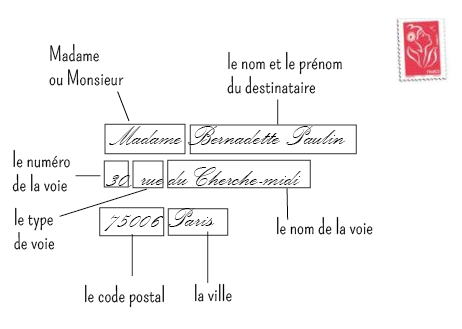
\includegraphics{./images/adresse-postale.png}
\caption{Modèle de rédaction correcte d'une adresse postale}
\end{figure}

La réalité ressemble souvent à celà

\begin{figure}
\centering
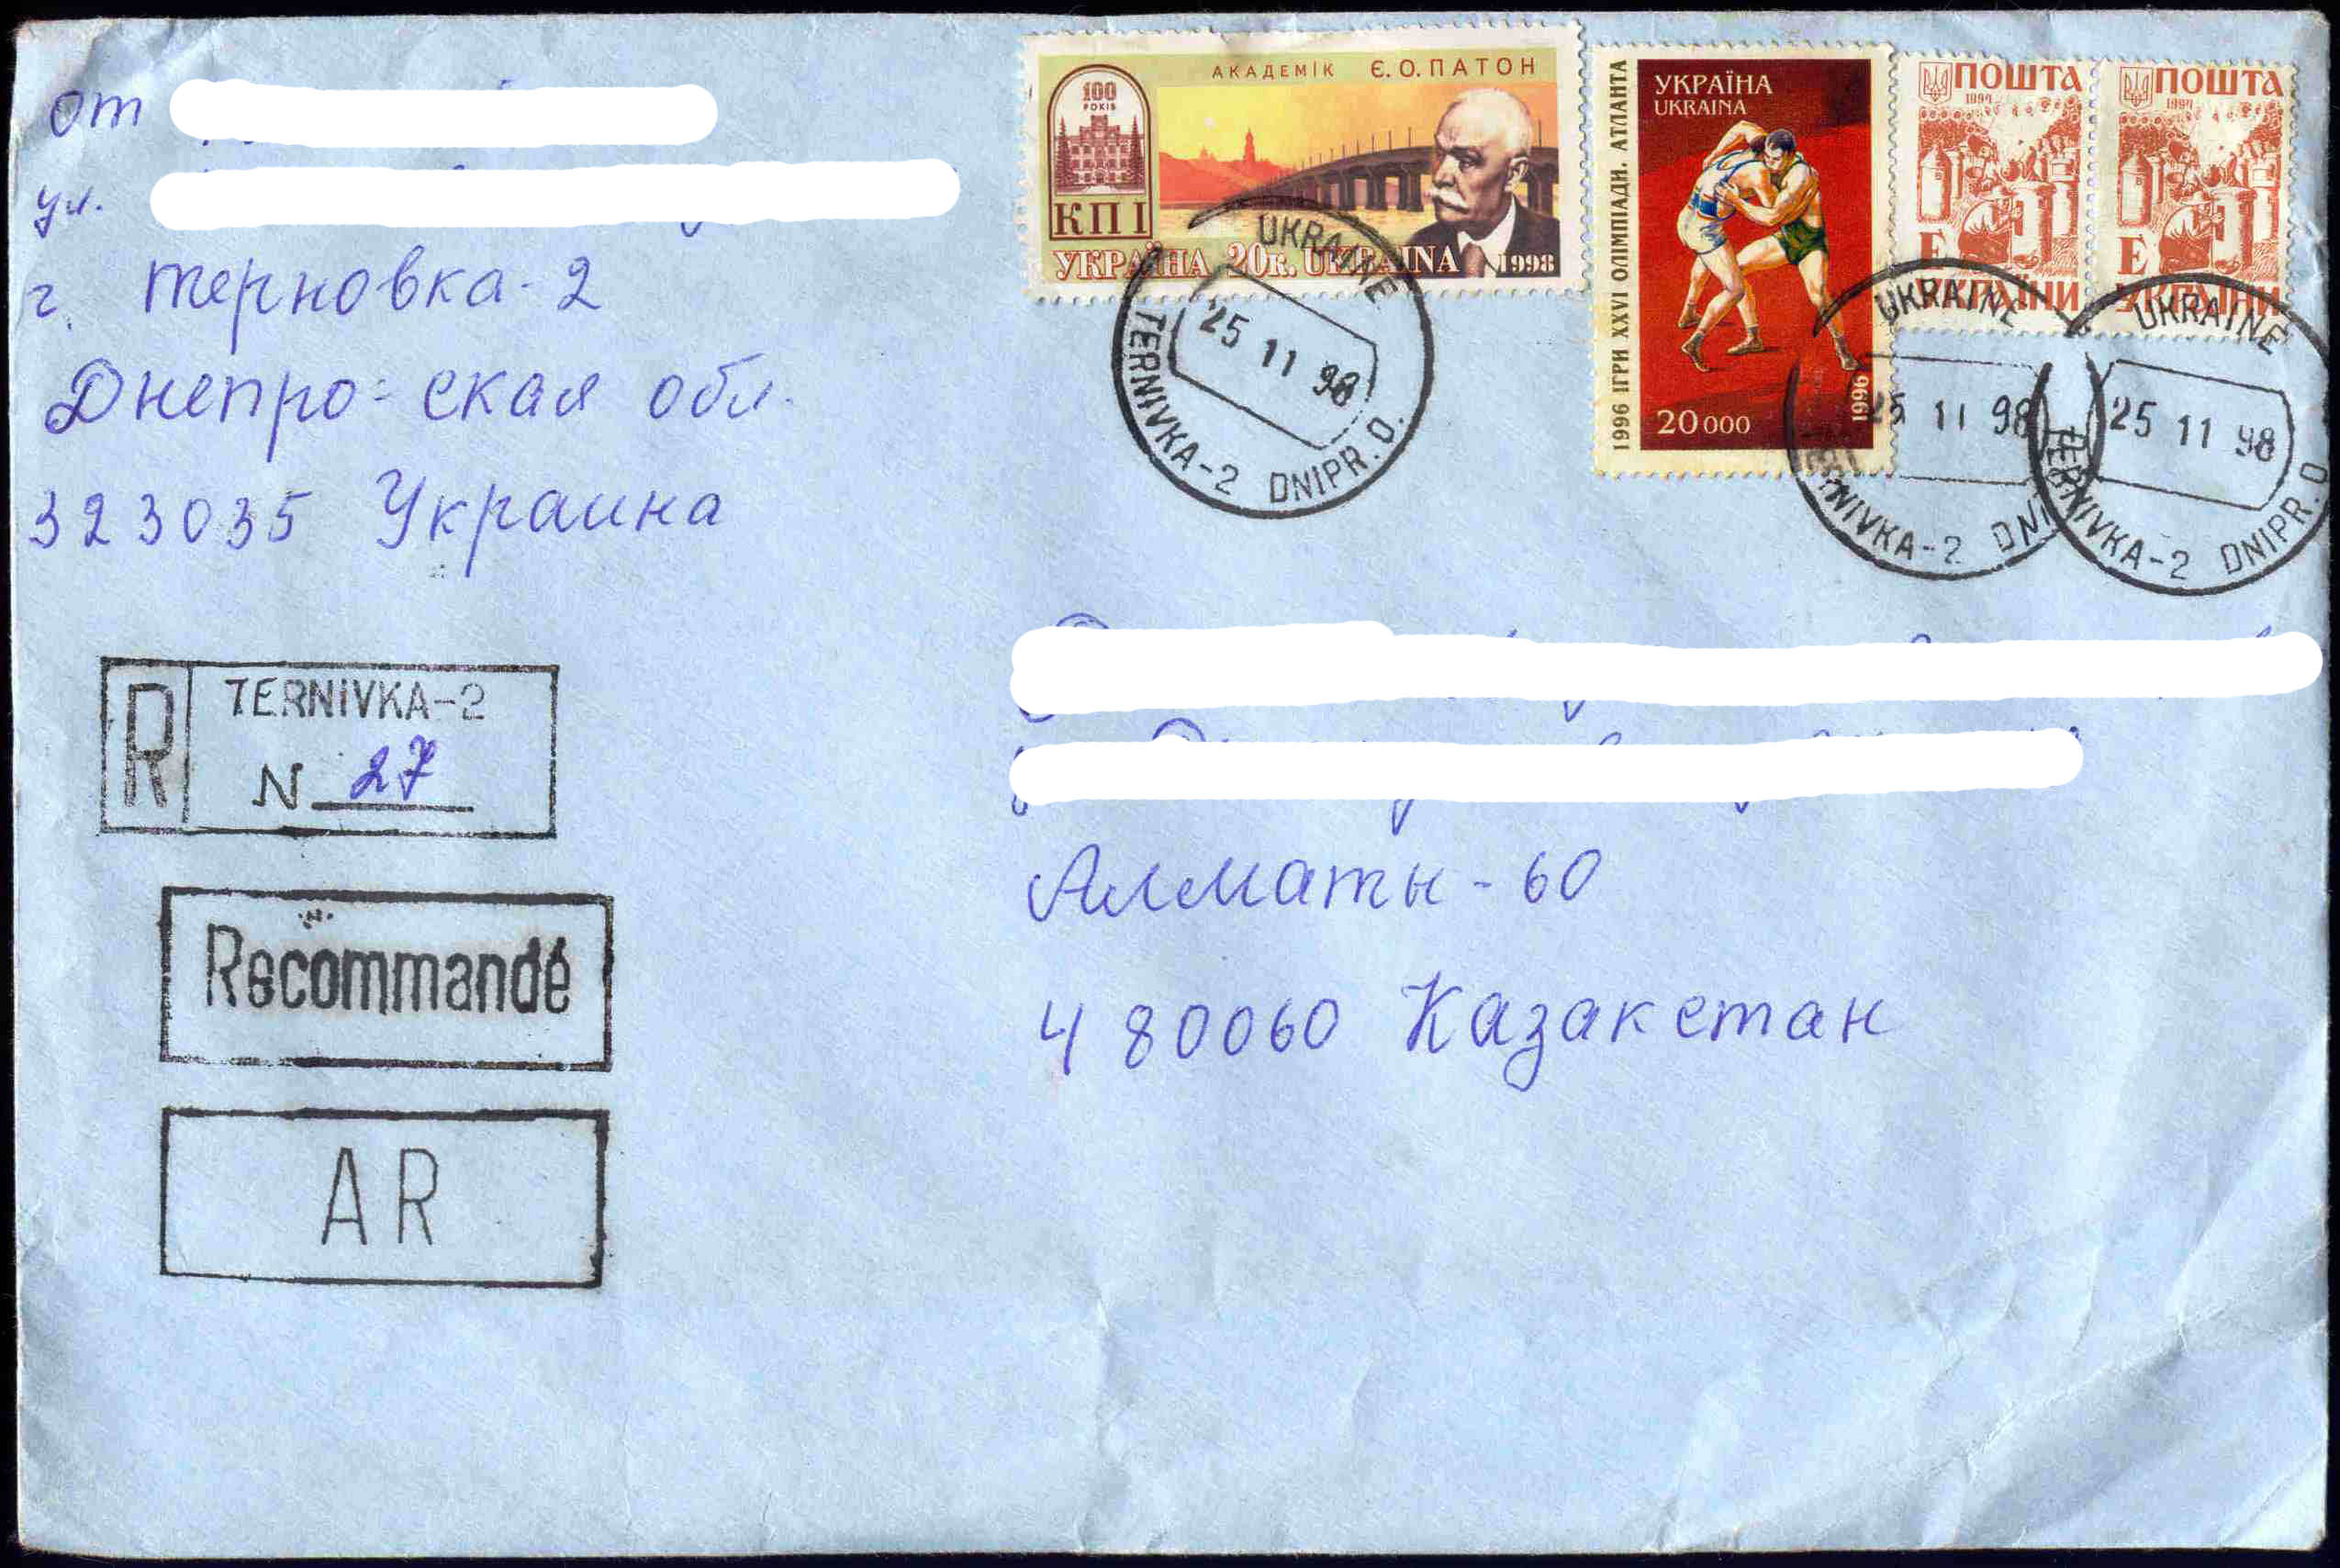
\includegraphics{./images/Posted_registered_letter_cover_Ukraine1998.jpg}
\caption{à çà}
\end{figure}

Dans un environnement en science sociale la situation est moins complexe, les documents analysés ne seront le plus souvent pas des documents mansuscrits ( sauf pour les médiévistes), mais le scan de document plus structurés. Par exemple les jpg

Une solution pour r est \href{https://cran.r-project.org/web/packages/tesseract/vignettes/intro.html}{tesseract}. C'est un package qui permet d'accéder au programme du même nom,développé à l'origine Chez Hewlett-Packard Laboratories entre 1985 et 1994, avec quelques modifications supplémentaires apportées en 1996 pour le portage sur Windows, et sur C en 1998.Tesseract a été mis en open Source par HP En 2005. Et de 2006 à novembre 2018, Google a continué a le développer.Il s'appuie sur des réseaux neuronaux de type LSTM. C'est une petite mais puissante intelligence artificielle qui supporte plus d'une centaine de langues.

Testons-le sans attendre avec le texte suivant.

\begin{figure}
\centering
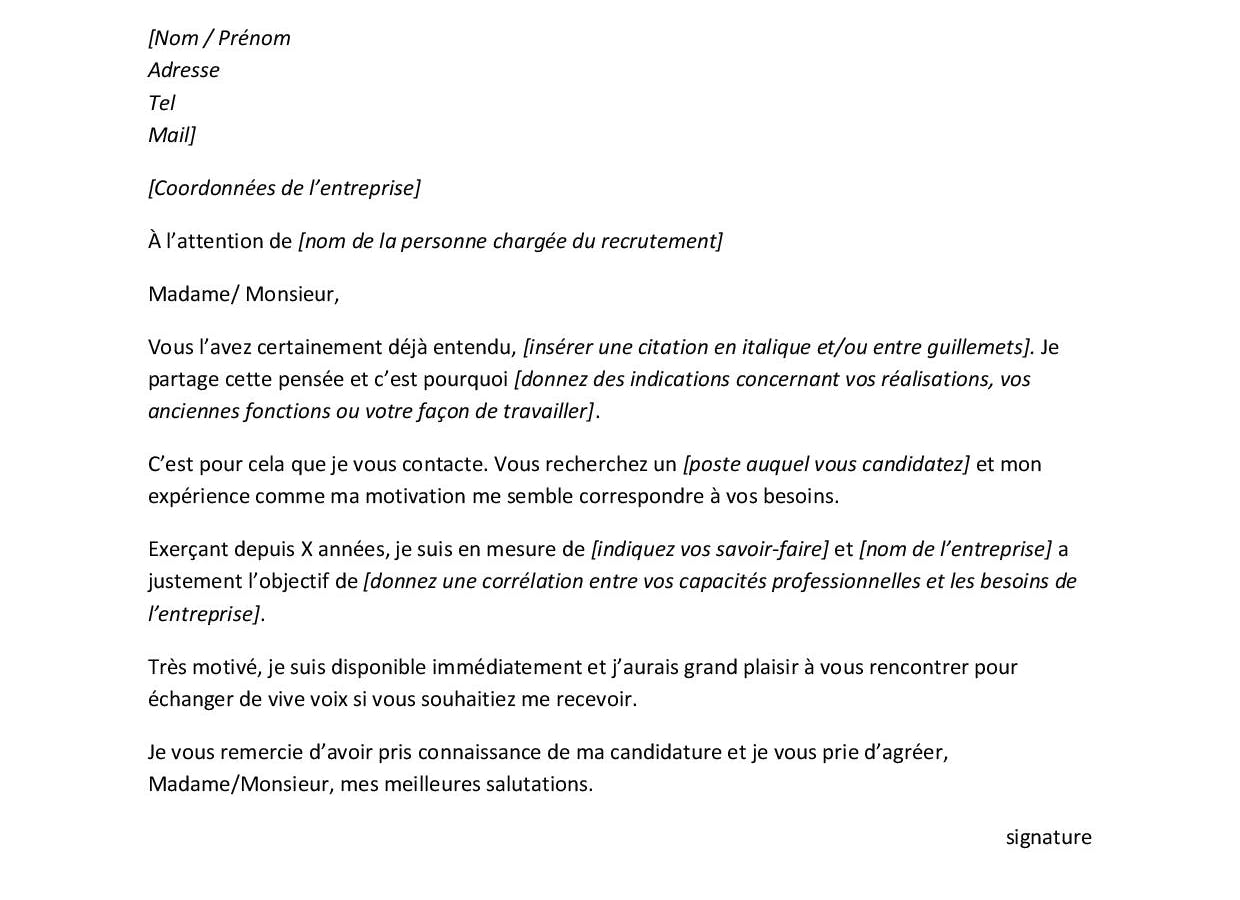
\includegraphics{./images/LettreMotivation.jpg}
\caption{Lettre de motivation}
\end{figure}

\url{https://gabriben.github.io/NLP.html\#introduction}

\begin{Shaded}
\begin{Highlighting}[]
\KeywordTok{library}\NormalTok{(tesseract)}

\CommentTok{#library(magick)#pour pré-traiter l'image et améliorer la reconnaissance}

\KeywordTok{tesseract_download}\NormalTok{(}\StringTok{"fra"}\NormalTok{) }\CommentTok{#pour télécharger le modèle de langage}
\end{Highlighting}
\end{Shaded}

\begin{verbatim}
## [1] "C:\\Users\\Super\\AppData\\Local\\tesseract4\\tesseract4\\tessdata/fra.traineddata"
\end{verbatim}

\begin{Shaded}
\begin{Highlighting}[]
\NormalTok{t1<-}\KeywordTok{Sys.time}\NormalTok{()}
\NormalTok{text <-}\StringTok{ }\NormalTok{tesseract}\OperatorTok{::}\KeywordTok{ocr}\NormalTok{(}\StringTok{"./images/LettreMotivation.jpg"}\NormalTok{, }\DataTypeTok{engine =} \StringTok{"fra"}\NormalTok{)}
\NormalTok{t2<-}\KeywordTok{Sys.time}\NormalTok{()}
\NormalTok{t<-}\StringTok{ }\NormalTok{t2}\OperatorTok{-}\NormalTok{t1}
\KeywordTok{cat}\NormalTok{(text)}
\end{Highlighting}
\end{Shaded}

\begin{verbatim}
## [Nom / Prénom
## Adresse
## Tel
## Mail]
## [Coordonnées de l’entreprise]
## À l'attention de {nom de la personne chargée du recrutement]
## Madame/ Monsieur,
## Vous l’avez certainement déjà entendu, [insérer une citation en italique et/ou entre guillemets]. Je
## partage cette pensée et c’est pourquoi [donnez des indications concernant vos réalisations, vos
## anciennes fonctions ou votre façon de travailler].
## C'est pour cela que je vous contacte. Vous recherchez un {poste auquel vous candidatez] et mon
## expérience comme ma motivation me semble correspondre à vos besoins.
## Exerçant depuis X années, je suis en mesure de {indiquez vos savoir-faire] et [nom de l’entreprise] a
## justement l’objectif de {donnez une corrélation entre vos capacités professionnelles et les besoins de
## l’entreprise].
## Très motivé, je suis disponible immédiatement et j'aurais grand plaisir à vous rencontrer pour
## échanger de vive voix si vous souhaitiez me recevoir.
## Je vous remercie d’avoir pris connaissance de ma candidature et je vous prie d’agréer,
## Madame/Monsieur, mes meilleures salutations.
## 
## signature
\end{verbatim}

\begin{Shaded}
\begin{Highlighting}[]
\CommentTok{#tesseract_info() #voir les langues disponibles}
\end{Highlighting}
\end{Shaded}

Pour améliorer la performance qui peut se mesurer au niveau des lettres mais doit surtout l'être au niveau des mots, deux stratégies sont possibles, la première de préprocessing, la seconde de postprocessing avec un mécanisme de détection et de correction d'erreur.

Le preprocessing consiste à traiter l'image en renforçant les contrastes , en éliminant le bruit, on en rend les pixels mieux digestes pour tesseract. C'est ce à quoi s'attache le pakage magick qui offre un bouquet de fonctions à cette fin. Nous laissons le lecteur le tester seul.

Le post-processing un introduire des mécanismes de correction d'erreurs au niveau des mots.Pour une idée de ce type de développement voir \href{https://gabriben.github.io/NLP.html}{Gabriel, Yadir, Xiaojie, Mingyu}

Naturellement, un paramètre important est la vitesse de traitement des images. Dans un projet complet on peut être amener à traiter des centaines images en boucle. Dans notre exemple la durée est de \texttt{t} secondes, autrement dit 6 images à la minute ou 360 à l'heure\ldots{}

\hypertarget{les-contenus-vocaux}{%
\section{Les contenus vocaux}\label{les-contenus-vocaux}}

La tradition méthodologique de la sociologie est celle de l'entretien, avec toute sorte d'acteur. Elle aboutit à la production de transcriptions, plus ou moins détaillées et précise. Mais des textes

On peut désormais enregistré des réaction par des interfaces vocales. le speech to text est de plus en plus efficace, voir l'API de google.

Il existe déja des packages sur r qui permettent d'accéder aux solutions de google langage qui necessite une clé d'API.

\url{https://cran.r-project.org/web/packages/googleLanguageR/vignettes/setup.html}

\hypertarget{echantillonner-le-texte}{%
\section{Echantillonner le texte}\label{echantillonner-le-texte}}

Un corpus reste un échantillon. Dans ce chapitre nous avons appris comment faire la cueillette dans les sources de textes et constituer matériellement un corpus. Il reste à traiter la question de la représentativité. La collecte doit rester raisonnée.

Les unités de texte. Une unité de texte : un chaine de caractère intégrée dans un document. Celui ci peut être un livre un article, une note, une transcription,

\begin{itemize}
\tightlist
\item
  Un document
\item
  Un ou des auteurs du document
\item
  Une date
\item
  Un endroit
\item
  Un contexte : les unités précedente, et subséquentes.
\end{itemize}

Unités de production et de reception, Un texte est produit et puis il est lu, peut-être.Analyser le texte peut se faire dans deux perspectives, celle de la production et celle de la réception. Les corpus doivent être construit en fonction de ce critère.

Examiner la question de l'engagement dans ce cadre est essentiel, certains acteurs sur un sujet donnée sont amenés à parler plus que les autres et développent un surcroit de voix. la question du biais de selection

Un corpus est un ensemble de documents. Ils peuvent être courts, les tweets, pas trop long - abstract articles court - long ( article de recherche, ou très long (livres).

La collecte peut se faire d'abord sur des matériaux primaires, numérisés sous forme d'images, et dans lesquels en analysant les pixels on peut reconnaitre un texte.

\hypertarget{conclusion-1}{%
\section{Conclusion}\label{conclusion-1}}

Dans ce chapitre nous aurons égratigné des sujets techniques de constitution de corpus en envisageant différents moyens d'acccès

\begin{itemize}
\tightlist
\item
  Scrapping
\item
  API
\item
  Pdf
\item
  texte dans les images
\item
  une ouverture à l'oral
\end{itemize}

On soulignera la technicité

On observera l'étendue des domaines à exploiter.

\hypertarget{visualiser-et-ruxe9duire-le-corpus}{%
\chapter{Visualiser et réduire le corpus}\label{visualiser-et-ruxe9duire-le-corpus}}

\hypertarget{explorer-le-corpus}{%
\section{Explorer le corpus}\label{explorer-le-corpus}}

(attention, c'est un chapitre qui doit être par la suite détaché)

Avant de procéder aux analyses du corpus, il est souvent utile de le représenter. On va utiliser le package Corpora explore à cette fin. Il permet de préparer un corpus et de le visualiser de manière interactive avec la génération d'une app shiny. Malheuresuement nous ne savons pas rendre compte de la dynamique de l'outil. On peut naviguer aisement dans l'ensemble de texte.

On va utiliser une collection de donnée préparée avec Manel Benzarafa de l'Université paris Nanterre, et qui comprend l'intégralité des résumés, auteurs etc.. relatifs aux articles publiés dans PMP. Une base bibliographique intégrale. 1025 articles la compose.

\begin{Shaded}
\begin{Highlighting}[]
\KeywordTok{library}\NormalTok{(readr)}
\CommentTok{#install.packages("corporaexplorer")}
\KeywordTok{library}\NormalTok{(corporaexplorer)}


\KeywordTok{library}\NormalTok{(readr)}
\NormalTok{PMP <-}\StringTok{ }\KeywordTok{read_csv}\NormalTok{(}\StringTok{"data/PMPLast.csv"}\NormalTok{)}

\NormalTok{PMP<-PMP }\OperatorTok\StringTok{ }
\StringTok{  }\KeywordTok{select}\NormalTok{(Key, Author, Title, Issue, }\DecValTok{3}\NormalTok{, }\DecValTok{11}\NormalTok{)}
\NormalTok{PMP<-PMP}\OperatorTok\StringTok{ }\KeywordTok{rename}\NormalTok{(}\DataTypeTok{Text=}\DecValTok{6}\NormalTok{, }\DataTypeTok{Annee=}\DecValTok{5}\NormalTok{) }\OperatorTok\StringTok{ }
\StringTok{  }\KeywordTok{filter}\NormalTok{(Text}\OperatorTok{!=}\StringTok{"Null"} \OperatorTok{&}\StringTok{ }\OperatorTok{!}\KeywordTok{is.na}\NormalTok{(Annee))}



\NormalTok{corpus <-}\StringTok{ }\KeywordTok{prepare_data}\NormalTok{(PMP,}
    \DataTypeTok{date_based_corpus =}\OtherTok{FALSE}\NormalTok{,}
    \DataTypeTok{grouping_variable =} \StringTok{"Annee"}\NormalTok{,                }\CommentTok{# change grouping variable}
 \DataTypeTok{within_group_identifier =} \StringTok{"Title"}\NormalTok{,}
 \DataTypeTok{columns_doc_info =}
        \KeywordTok{colnames}\NormalTok{(df)[}\DecValTok{1}\OperatorTok{:}\DecValTok{4}\NormalTok{],}
 \DataTypeTok{tile_length_range =} \KeywordTok{c}\NormalTok{(}\DecValTok{2}\NormalTok{, }\DecValTok{10}\NormalTok{),}
    \DataTypeTok{use_matrix =} \OtherTok{FALSE}
\NormalTok{)}
\CommentTok{#explore(corpus)}
\end{Highlighting}
\end{Shaded}

Dans la photo d'écran suivante, on teste les termes " politique" et ``management''. Chaque tuile ( tile) représente un des 1025 abstracts qui composent le corpus. Les couleurs correspondent à la fréquence des deux termes.

\begin{figure}
\centering
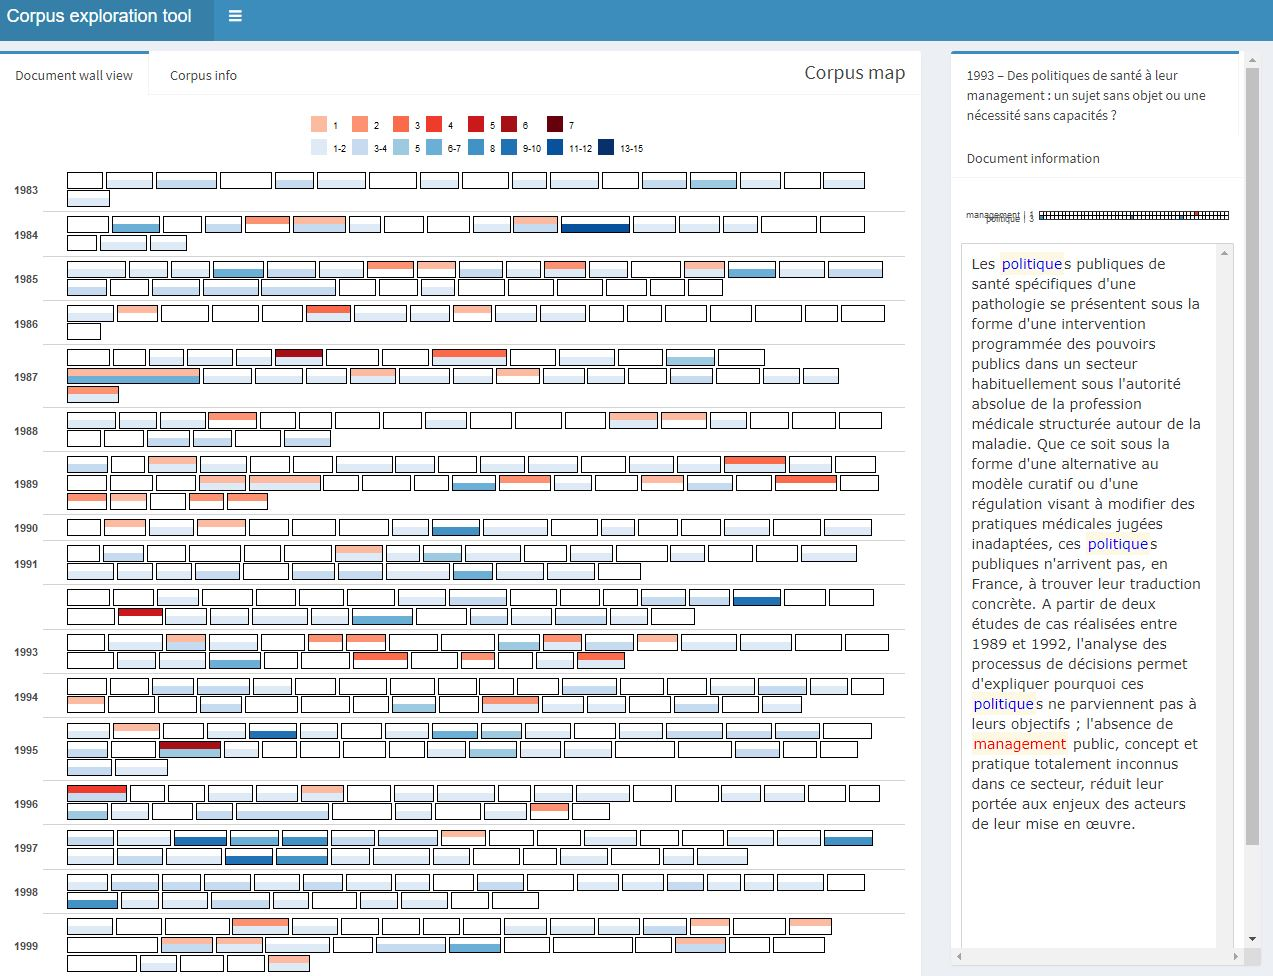
\includegraphics{./images/Corporaexplore.jpg}
\caption{Exploration des abstracts de PMP}
\end{figure}

\hypertarget{pruxe9paration-des-donnuxe9es}{%
\chapter{Préparation des données}\label{pruxe9paration-des-donnuxe9es}}

Avant de se lancer dans l'analyse, il est nécessaire de préparer le texte, de le pré-traiter. Son format fondamental est celui d'une chaine de caractères, sans signification particulière mais composé à partir d'un alphbat, c'un jeux de signes déterminés et démobralement. 1/0 pour lelangage bianre, AGCP pour l'adan, 26 caractère de base pour l'alphabet, sans compter les accents.

Ces variations sont l'objet de convention en informatique. et de certaines opérations.

traiter du texte c'est avant tout disposer d'opérateurs pour manipuler ces éléments élémentaire. la base est d'avoir des outils pour les manipuler.

Le langage avant d'être signifiant est signifié, littéralement produit comme une chaine de signes qui dans l'usage suit certaine convention. Par exemple la satisfaction peut s'exprimé par mmmm, une forte satisfaction par un mmmmmmmmmmmmmmmmmmmmm. Pour distinguer les significations, il faut d'abord compter. les mmm sont sans doute courants car conventionnels (ce mot est à deux doigts d'être incorporé au dictionnaire de l'Académie Française, s'il n'était qu'une onomatopée), les ``mmmmmmmmmmmmmmmmmmmmm'' sont sans doute beaucoups plus rares. De plus on trouvera des ``hum'' des ``hummm'', des 'mmmmhummmm". On comprend qu'à la nuance de l'intensité que le locuteur veut exprimer, toute ces morphologies se rapportent à une même idée.

Comment le rammener à une même formes est une question essentielle même si elle semble excessivement technique.

\hypertarget{manipuler-des-chaines-de-caractuxe8res}{%
\section{Manipuler des chaines de caractères}\label{manipuler-des-chaines-de-caractuxe8res}}

Il faut donc traiter le texte, avant même de s'engager dans des modèles compliqués. Il faut savoir traiter des chaines de caractères pour en réduire la diversité, et en produire des chaines grammaticalement exacte. C'est un travail d'artisan, celui des des imprimeurs et de leurs coorecteur. Et en particulier d'un métier celui du \href{http://www.textesrares.com/dupon/d376.htm}{compositeur}, ou ouvrier de la casse, qui distribue des caractères de plomb en séquences dans des casiers de bois.

\href{\%22./data/compositeur.jpg\%22}{cmpositeur}

L'artisan n'avait pas de choix, la précision était essentielle pour éviter la coquille. Le texte moderne, numérique, est l'objet de plus d'aller et retours. Les mots qu'on pianotent sont corrigés avant même d'être frappés. Les gestes techniques sont différents mais s'articulent sur une même idée : la langue écrite, du moins les langues alphabétiques sont des chaines de caractères dont la formation suit des règles fluctuantes à travers l'histoire mais contraignante à chaque moments. Les conventiosn peuvent changer, mais dans son temps elle s'imposent définitivement. Personne n'écrirait ``deffert'', pour dire ``dessert''. Et pourtant la graphie du s était un f jusqu'au XVI ème siècle (trouver la source)!
\url{https://www.cairn.info/revue-la-linguistique-2003-1-page-3.htm}

De nombreuses ressources sont disponibles pour traiter ces chaines de caractères.

On utilisera surtout \href{https://stringr.tidyverse.org/}{Stringer} qui est est un des composants essentiels de tidyverse. D'autres packages sont équivalents : stringi par exemple.

\hypertarget{les-opuxe9rations-sur-les-chauxeenes-de-caractuxe8res}{%
\subsection{Les opérations sur les chaînes de caractères}\label{les-opuxe9rations-sur-les-chauxeenes-de-caractuxe8res}}

\begin{itemize}
\tightlist
\item
  mettre en minuscule. L'alphabet se présente au moins en deux versions : des majuscules et des minuscules, il est souvent nécessaire de réduire le texte à une seule casse pour en réduire la variété, sauf si les majuscules signalent une information spécifique et socialement conventionnelle. Un mot qui débute par une majuscule signale un nom commun, désormais conceptualisé comme une entité nommée appartenant à différentes catégories : noms de lieux, noms de personnes, noms d'organisation \ldots ou l'expression d'un sentiment, au sein des chats, la majuscule en série signale un niveau de langage ``loud'', un cri , une engueulade, la véhémence.\\
\item
  rechercher une chaine de caractères;
\item
  remplacer une chaine de caractères
\item
  extraire une chaine de caractère d'un emplacement à l'autre
\item
  supprimer une chaine de caractères. Les nombres,
\item
  concaténer des chaines de caractères. Le texte peut être divisés en unités. Un paragraphe par exemple, ou un titre.
\end{itemize}

Si la manipulation deslaquelle ? vaccin ?

\hypertarget{la-technique-des-expressions-ruxe9guliuxe8res-regex}{%
\subsection{La technique des expressions régulières (regex)}\label{la-technique-des-expressions-ruxe9guliuxe8res-regex}}

Il ne suffit pas de chercher une chaine de caractère particulière, il faut souvent saisir un ensemble de variations qui suivent un motif determiné et qui répond à une sorte de loi générale.

Par exemple si je veux retrouvrer dans un corpus l'ensemble des mots relatif au monde de l'hôpital, nous chercherions aussi le mot ``hopital''. Nombreux seront les locuteur qui omeetent l'accent circonflexe. Une formule pour trouver ces deux varietés serait d'utiliser un opérateur, "(), pour définir une option . soit l'un soit l'autre :
h(ô,o)pital

Une expression régulière est un masque qui permet d'identifier des formes principales et leurs variétés. Il s'appuit sur une codification dont quelques éléments clés permettent de se donner une bonne idée de la logique générale

\begin{itemize}
\item
  le \^{}, indique que la forme commence par le caractère qui suit ``\^{}A''
\item
  le . signifie n'importe quel caractère. le regex ``\^{}a.'' signifiera ainsi n'importe quelle chaine de caractère qui commence par a est est suivi de n'importe quel caractère.
\item
  le * la répétition indéfinie du caractère .
\end{itemize}

D'un point de vue linguistique les regex travaillent sur la morphologie et ses variations, indépendemment des règles de grammaires mais profitant de leur régularité.

Les mots sont généralement composés d'une racine, de suffixe et de préfixe qui contiennent les flexions grammaticales et sémantiques.

des exemples :

\begin{itemize}
\tightlist
\item
  la négation : visible et in-visible.
\item
  la conjugaison : aime et aim-ât
\item
  la numération : fraise et fraise-s
\item
  le genre : épicier et épicière-s.
\end{itemize}

\hypertarget{un-fondement-profond-et-ancien}{%
\subsection{Un fondement profond et ancien}\label{un-fondement-profond-et-ancien}}

Le langage des regex a répondu d'abord aux besoin des informaticiens, et s'appuie sur une construction mathématique sophistiquée : les automatates finis
\url{https://swtch.com/~rsc/regexp/regexp1.html} don t un des contributeurs essentiels à été

doi.org/10.1145/363347.363387 Ken Thompson

fondateur de Grepl

a method for locating specific character strings embedded in character text is described and an implementation of this method in the form of a compiler is discussed. The compiler accepts a regular expression as source language and produces an IBM 7094 program as object language. The object program then accepts the text to be searched as input and produces a signal every time an embedded string in the text matches the given regular expression. Examples, problems, and solutions are also presented.

\url{https://swtch.com/~rsc/regexp/regexp1.html}

\hypertarget{des-applications-truxe8s-pratiques}{%
\subsection{Des applications très pratiques}\label{des-applications-truxe8s-pratiques}}

et à ceux qui face à des questions de métier, par exemple les professionnel de marketing direct ou des services postaux, ont été amené à traiter de jeux de données textuels limités tel qu'une adresse postale.

\begin{itemize}
\item
  dectecter une entité nommée : la majuscule
\item
  détecter une adresse
\item
  détecter une date
\item
  détecter un compte
\item
  détecter une url
\end{itemize}

\hypertarget{nettoyer-le-texte}{%
\section{Nettoyer le texte}\label{nettoyer-le-texte}}

\begin{itemize}
\tightlist
\item
  enlever les mentions
\item
  enlever les url
\item
  enlever ou recoder les emojis
\item
  enlever la ponctuation
\item
  enlever les nombres
\end{itemize}

\hypertarget{corriger-le-texte}{%
\section{Corriger le texte}\label{corriger-le-texte}}

Si certains corpus sont par les conditions de leur production presque parfait du point de vue grammatical et lexical, c'est le cas en principe des articles de presse et des documents officiels, d'autres qui s'appuient sur une langue vernaculaire on des graphies plus incertaines et des syntaxes approximatives. Dans un tiers des cas le mot " opinion" s'orthographie ``opignons''. Chaque mot du lexique s'évanouit dans des morphologies nombreuses et approximatives.

C'est un obstacle à l'analyse car la variété morphologique est aléatoire.

plusieurs stratégies sont possibles. La première est de corriger le texte notamment en employant des outils de corrections efficaces.

\hypertarget{la-correction-orthographique-automatique}{%
\subsection{La correction orthographique automatique}\label{la-correction-orthographique-automatique}}

voir hunspell

\url{https://cran.r-project.org/web/packages/hunspell/vignettes/intro.html\#Custom_Dictionaries}

\hypertarget{analyse-cibluxe9e-par-les-regex}{%
\subsection{Analyse ciblée par les regex}\label{analyse-cibluxe9e-par-les-regex}}

Une application des regex est l'analyse ciblée d'un certain nombre de termes. LA corection est partielle mais couvre les cibles essentielles

exemple des gestes barières dans le flux twitter

\hypertarget{identifier-les-sources}{%
\section{Identifier les sources}\label{identifier-les-sources}}

Dans l'analyse des contenus sociaux, les textes viennent de sources multiples et confuses. Elles peuvent être aisément multilingue. Analyser un corpus d'entretien, une collection de discours, posent peu la questions des locuteurs car ils sont bien identifiés. Ce n'est pas le cas dans les réseaux sociaux où les buts sont multiples et plus ou moins avoués.

Les acteurs :

\begin{itemize}
\tightlist
\item
  des professionnels de la politiques et les institutions qu'ils dirigent
\item
  Journaliste et professionnels de la communication
\item
  Experts et universitaires
\item
  les marques et leur community manager
\item
  les bots
\item
  les trolls
\item
  les activistes
\end{itemize}

\hypertarget{identifier-la-langue}{%
\subsection{Identifier la langue}\label{identifier-la-langue}}

Dans les points précedents on suppose que la langue est homogène, mais les corpus peuvent être multi-langues. Par exemple, dans les corpus d'avis d'hôtes sur Airbnb, les avis sont formulés dans une large variété de langues. Il va falloir en tenir compte et une tâche préliminaire sera de détecter les langues pour séparer les corpus.

Le package textcat offre une solution basée sur la fréquence des ngrams (voir chapitre x). et compare la distribution du texte ciblée avec les distributions typiques des langues. Google propose un algo cpd3(\url{https://github.com/google/cld3}) plus sophistiqués dans la mesure où c'est un réseau de neurones qui fait le travail. Comparons les.

On utilise un jeu de donnée Airbnb sur Bruxelles qui accueillant les institutions européennnes est une des villes les plus cosmopolite qui soit avec des fonctionnaires venant de toutes l'europe et s'exprimant dans une large variété de langue, sans compter les représentations des autres pays du monde.

En terme de durée de calcul, la différence en temps de calcul est faramineuse 7 secondes contre 7 minutes, ce qui s'explique car texcat s'appuyant sur la distribution des ngrams doit les calculer pour les 36000 observations que nous avons retenues.

Faisons un test sur un extrait du corpus Airbnb.

\begin{Shaded}
\begin{Highlighting}[]
\NormalTok{BXL2021 <-}\StringTok{ }\KeywordTok{read_csv}\NormalTok{(}\StringTok{"./data/reviewsBXL2021.csv"}\NormalTok{)}
\NormalTok{BXL2021}\OperatorTok{$}\NormalTok{Year<-}\StringTok{ }\KeywordTok{as.numeric}\NormalTok{(}\KeywordTok{format}\NormalTok{(}\KeywordTok{as.Date}\NormalTok{(BXL2021}\OperatorTok{$}\NormalTok{date, }\DataTypeTok{format=}\StringTok{"%Y-%m-%d"}\NormalTok{),}\StringTok{"%Y"}\NormalTok{))}

\NormalTok{BXL2021<-}\StringTok{ }\NormalTok{BXL2021 }\OperatorTok\StringTok{ }\KeywordTok{filter}\NormalTok{(Year}\OperatorTok{>}\DecValTok{2019}\NormalTok{) }\CommentTok{# on filtre sur la période de confinement}

\KeywordTok{library}\NormalTok{(cld3)}

\NormalTok{t1<-}\KeywordTok{Sys.time}\NormalTok{()}

\NormalTok{cld3<-}\KeywordTok{as.data.frame}\NormalTok{(}\KeywordTok{detect_language}\NormalTok{(BXL2021}\OperatorTok{$}\NormalTok{comments))}\OperatorTok\KeywordTok{rename}\NormalTok{(}\DataTypeTok{cld3=}\DecValTok{1}\NormalTok{)}
\NormalTok{t2<-}\KeywordTok{Sys.time}\NormalTok{()}

\NormalTok{t_cld3<-t2}\OperatorTok{-}\NormalTok{t1 }\CommentTok{#on calcule la durée de l'opération en faisant la différence du temps de départ et d'arrivée}

\KeywordTok{library}\NormalTok{(textcat)}
\NormalTok{t1<-}\KeywordTok{Sys.time}\NormalTok{()}
\NormalTok{textcat<-}\KeywordTok{textcat}\NormalTok{(BXL2021}\OperatorTok{$}\NormalTok{comments)}
\NormalTok{t2<-}\KeywordTok{Sys.time}\NormalTok{()}
\NormalTok{t_texcat<-t2}\OperatorTok{-}\NormalTok{t1}
\NormalTok{foo<-}\KeywordTok{cbind}\NormalTok{(cld3, textcat)}
\end{Highlighting}
\end{Shaded}

Examinons les résultats et la distribution des langues identifiées par les deux systèmes. Si l'ordre est respecté, des différences s'observent, \texttt{cld3} identifie du chinois qui ne fait pas partie du répertoire de texcat.

\begin{Shaded}
\begin{Highlighting}[]
\NormalTok{g1<-foo}\OperatorTok\KeywordTok{mutate}\NormalTok{(}\DataTypeTok{n=}\DecValTok{1}\NormalTok{)}\OperatorTok\KeywordTok{group_by}\NormalTok{(textcat)}\OperatorTok\KeywordTok{summarise}\NormalTok{(}\DataTypeTok{n=}\KeywordTok{sum}\NormalTok{(n))}\OperatorTok
\StringTok{  }\KeywordTok{ggplot}\NormalTok{(}\KeywordTok{aes}\NormalTok{(}\DataTypeTok{x=}\KeywordTok{reorder}\NormalTok{(textcat,n), }\DataTypeTok{y=}\NormalTok{n))}\OperatorTok{+}\KeywordTok{geom_bar}\NormalTok{(}\DataTypeTok{stat=}\StringTok{"identity"}\NormalTok{)}\OperatorTok{+}\KeywordTok{coord_flip}\NormalTok{()}\OperatorTok{+}\KeywordTok{scale_y_log10}\NormalTok{()}

\NormalTok{g2<-foo}\OperatorTok\KeywordTok{mutate}\NormalTok{(}\DataTypeTok{n=}\DecValTok{1}\NormalTok{)}\OperatorTok
\StringTok{  }\KeywordTok{group_by}\NormalTok{(cld3)}\OperatorTok
\StringTok{  }\KeywordTok{summarise}\NormalTok{(}\DataTypeTok{n=}\KeywordTok{sum}\NormalTok{(n))}\OperatorTok
\StringTok{  }\KeywordTok{ggplot}\NormalTok{(}\KeywordTok{aes}\NormalTok{(}\DataTypeTok{x=}\KeywordTok{reorder}\NormalTok{(cld3,n), }\DataTypeTok{y=}\NormalTok{n))}\OperatorTok{+}\StringTok{ }\KeywordTok{geom_bar}\NormalTok{(}\DataTypeTok{stat=}\StringTok{"identity"}\NormalTok{)}\OperatorTok{+}\KeywordTok{coord_flip}\NormalTok{()}\OperatorTok{+}\KeywordTok{scale_y_log10}\NormalTok{()}

\KeywordTok{plot_grid}\NormalTok{(g1, g2, }\DataTypeTok{labels =} \KeywordTok{c}\NormalTok{(}\StringTok{'Texcat'}\NormalTok{,}\StringTok{'Cld3'}\NormalTok{), }\DataTypeTok{label_size =} \DecValTok{12}\NormalTok{)}
\end{Highlighting}
\end{Shaded}

\begin{figure}

{\centering 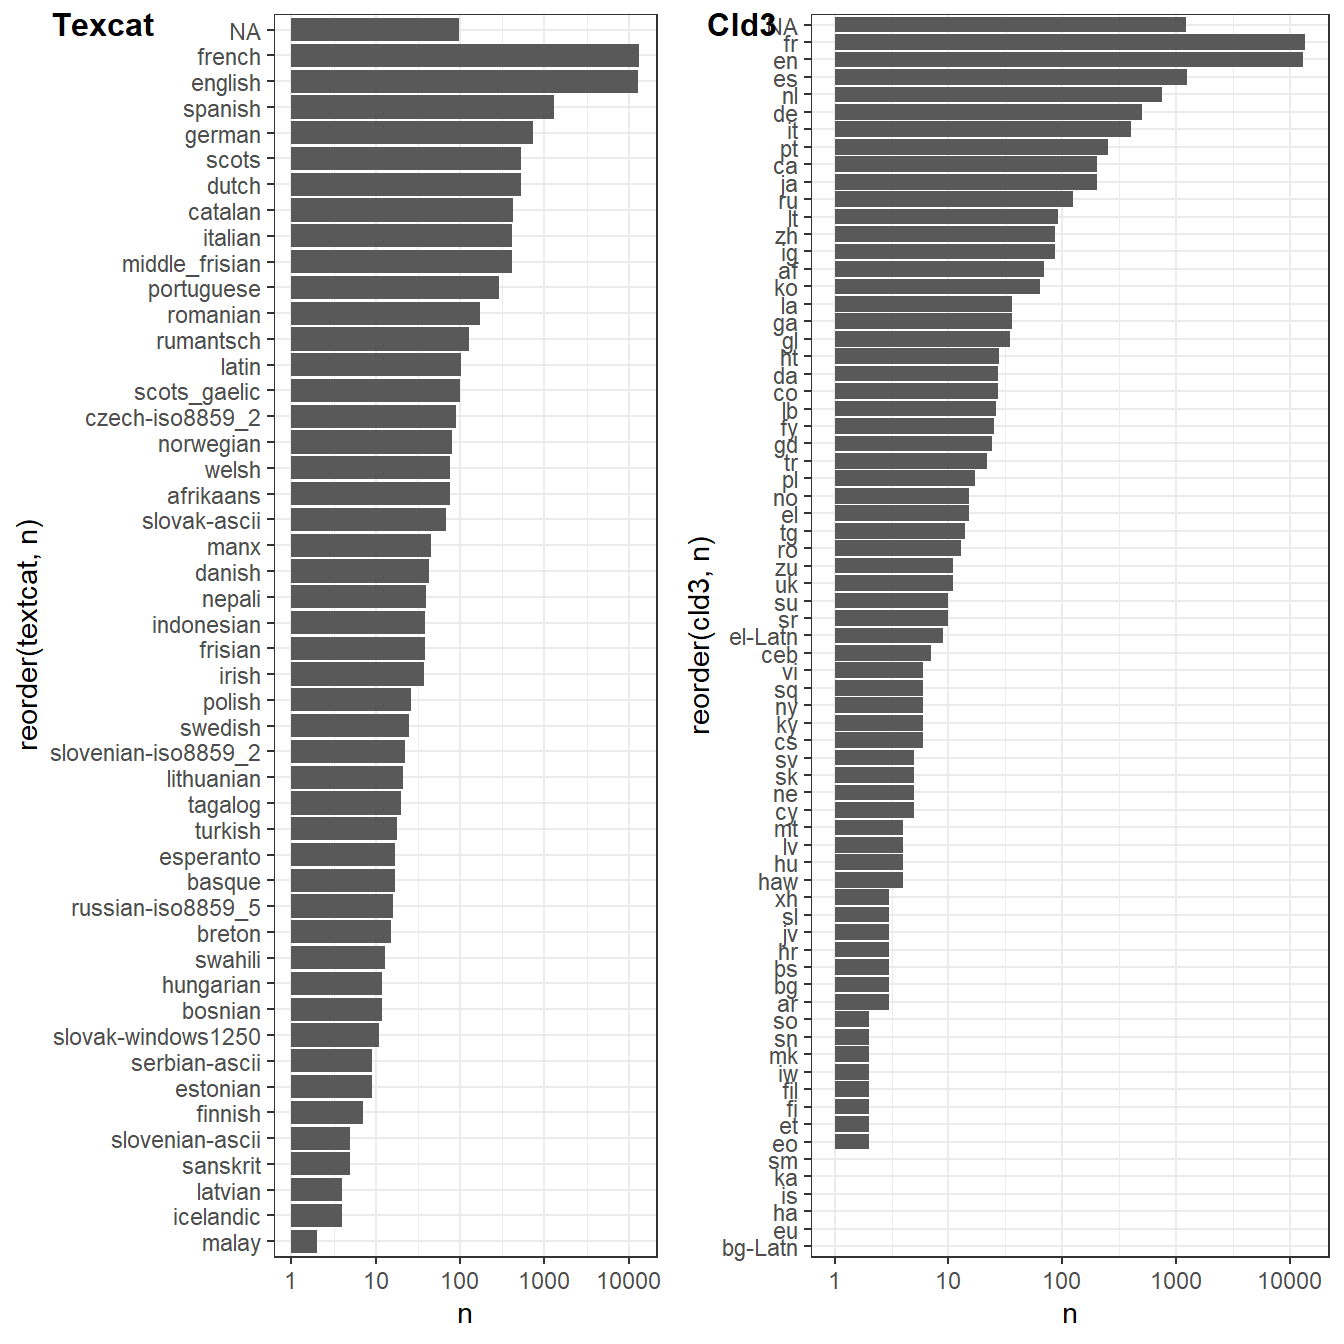
\includegraphics[width=0.8\linewidth]{bookdown-demo_files/figure-latex/302-1} 

}

\end{figure}

Examions maintenant la convergence des méthodes en représentant la répartition du résultat d'un système dans les langue de l'autre. Si la convergence est parfaite 1000\% des textes classé en Français par Textact devrait se retrouver dans 100\% de ces textes classé par cld3 et réciproquement.

\begin{Shaded}
\begin{Highlighting}[]
\NormalTok{foo1 <-foo }\OperatorTok\StringTok{ }\KeywordTok{mutate}\NormalTok{(}\DataTypeTok{n=}\DecValTok{1}\NormalTok{)}\OperatorTok\KeywordTok{group_by}\NormalTok{(textcat) }\OperatorTok\KeywordTok{summarise}\NormalTok{(}\DataTypeTok{n=}\KeywordTok{sum}\NormalTok{(n))}
\NormalTok{foo1<-foo}\OperatorTok\StringTok{ }\KeywordTok{left_join}\NormalTok{(foo1) }\OperatorTok\StringTok{ }\KeywordTok{filter}\NormalTok{(n}\OperatorTok{>}\DecValTok{10}\NormalTok{)}

\NormalTok{table<-}\KeywordTok{table}\NormalTok{(foo1}\OperatorTok{$}\NormalTok{cld3,foo1}\OperatorTok{$}\NormalTok{textcat)}
\NormalTok{foo1<-}\KeywordTok{as.data.frame}\NormalTok{(}\KeywordTok{prop.table}\NormalTok{(table,}\DecValTok{2}\NormalTok{))}


\KeywordTok{ggplot}\NormalTok{(foo1, }\KeywordTok{aes}\NormalTok{(}\KeywordTok{reorder}\NormalTok{(Var2, Freq),Var1)) }\OperatorTok{+}\StringTok{ }
\StringTok{  }\KeywordTok{geom_tile}\NormalTok{(}\KeywordTok{aes}\NormalTok{(}\DataTypeTok{fill =}\NormalTok{ Freq)) }\OperatorTok{+}\StringTok{ }
\StringTok{  }\KeywordTok{scale_fill_gradient}\NormalTok{(}\DataTypeTok{low =} \StringTok{"White"}\NormalTok{,}\DataTypeTok{high =} \StringTok{"Blue"}\NormalTok{)}\OperatorTok{+}
\StringTok{  }\KeywordTok{theme_bw}\NormalTok{()}\OperatorTok{+}\StringTok{ }\KeywordTok{theme}\NormalTok{(}\DataTypeTok{axis.text.x=}\KeywordTok{element_text}\NormalTok{(}\DataTypeTok{angle =} \DecValTok{45}\NormalTok{, }\DataTypeTok{hjust =}\DecValTok{1}\NormalTok{))}\OperatorTok{+}\KeywordTok{coord_flip}\NormalTok{()}
\end{Highlighting}
\end{Shaded}

\begin{figure}

{\centering 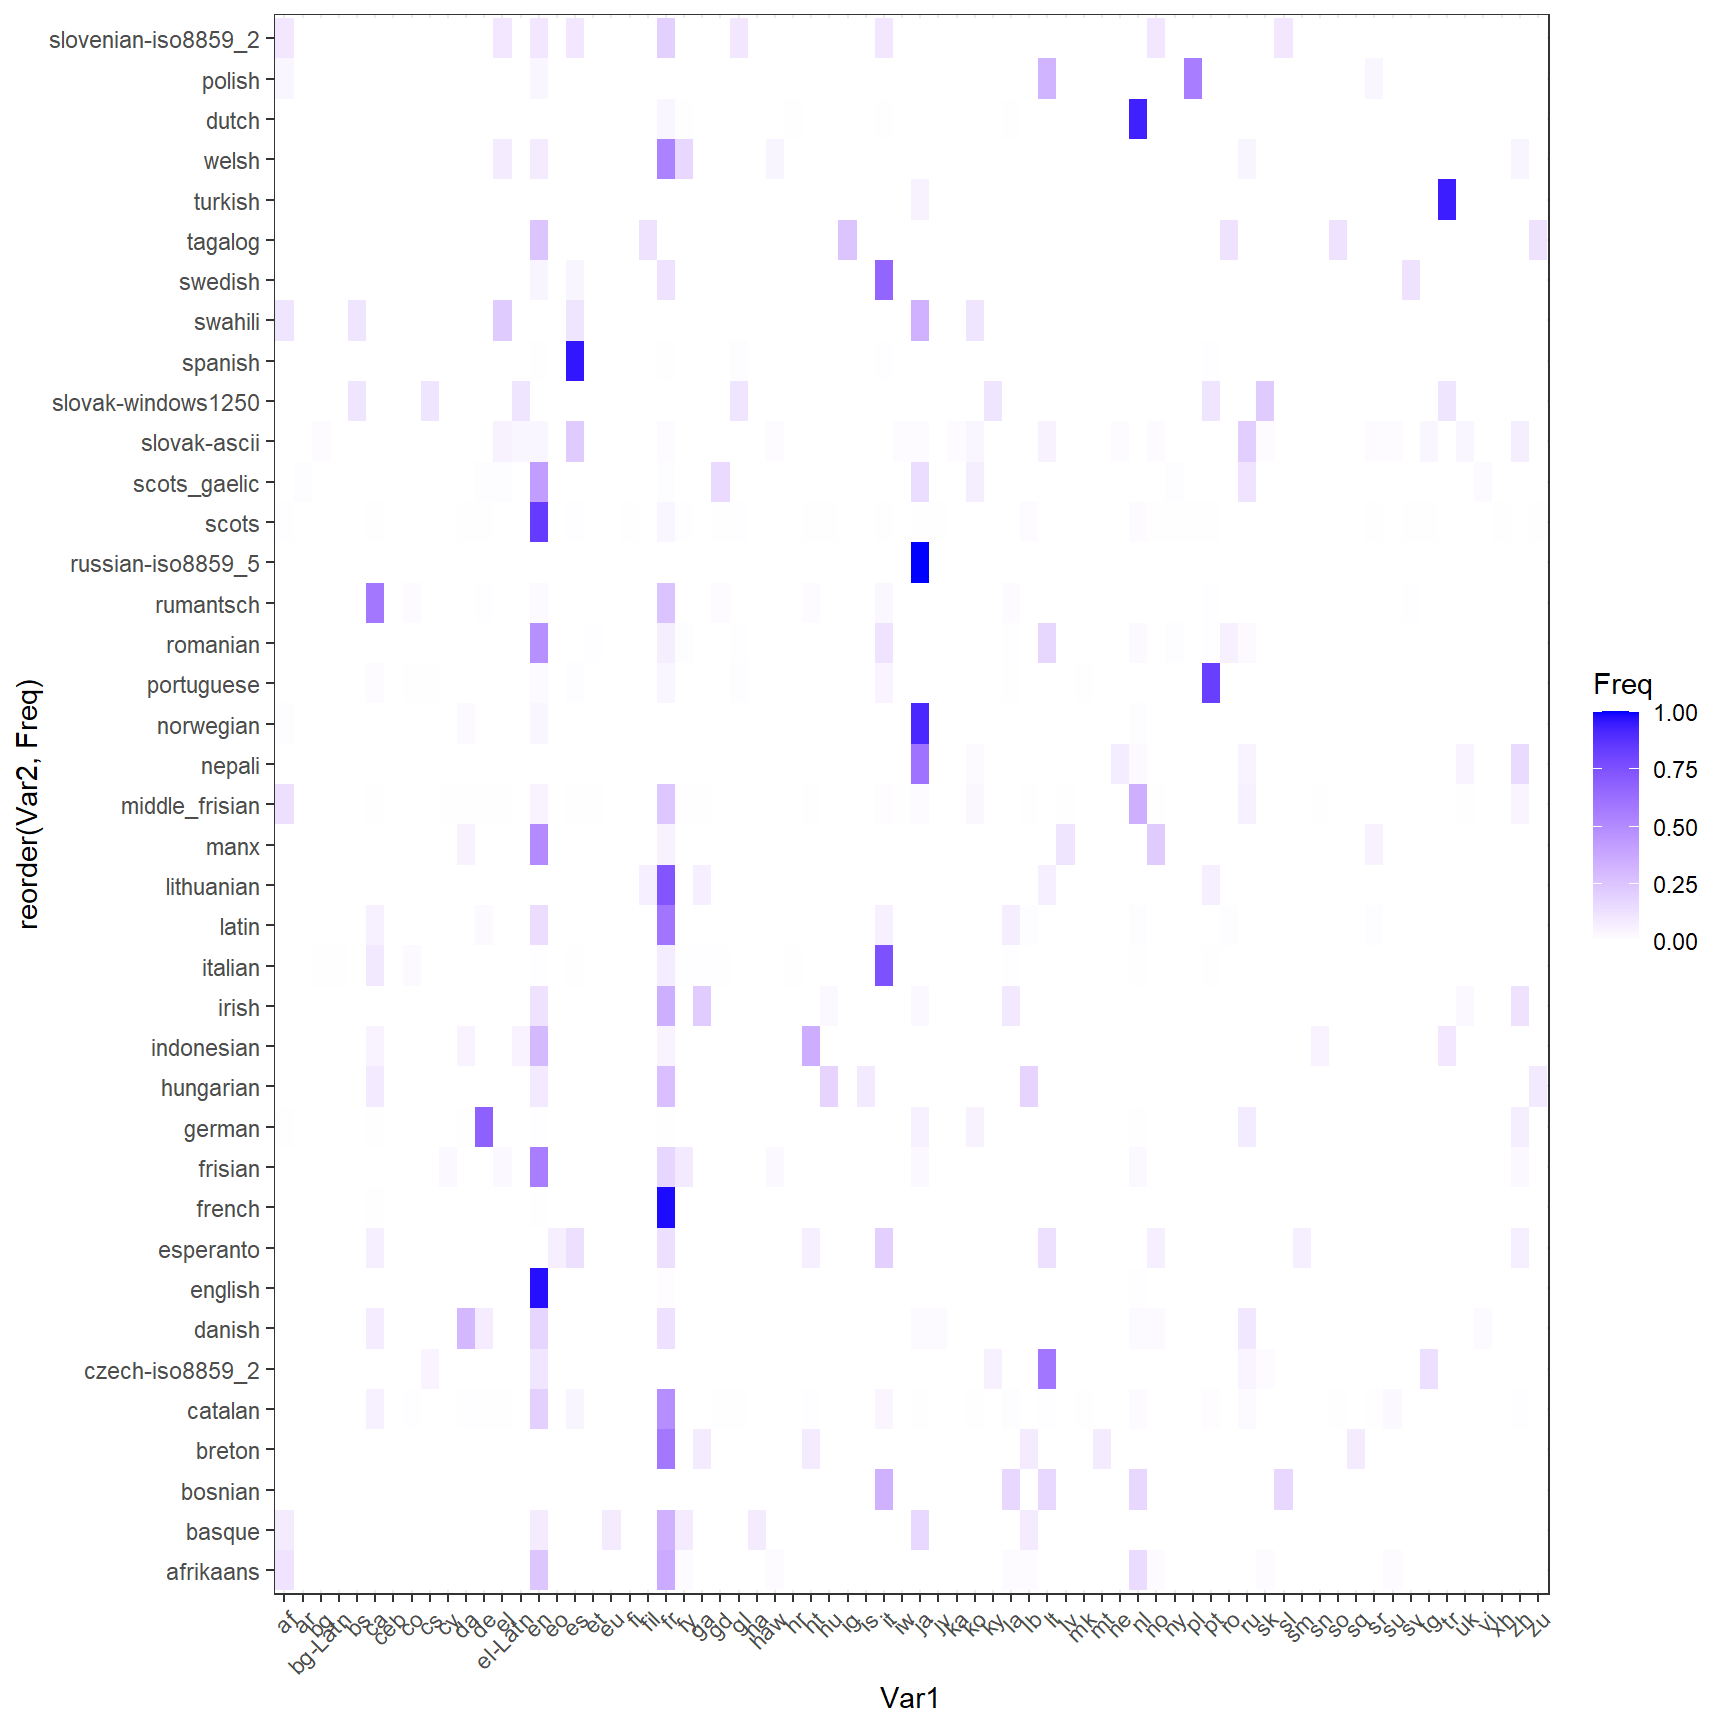
\includegraphics[width=0.8\linewidth]{bookdown-demo_files/figure-latex/303-1} 

}

\end{figure}

\begin{Shaded}
\begin{Highlighting}[]
\NormalTok{foo1 <-foo }\OperatorTok\StringTok{ }\KeywordTok{mutate}\NormalTok{(}\DataTypeTok{n=}\DecValTok{1}\NormalTok{)}\OperatorTok\KeywordTok{group_by}\NormalTok{(cld3) }\OperatorTok\KeywordTok{summarise}\NormalTok{(}\DataTypeTok{n=}\KeywordTok{sum}\NormalTok{(n))}
\NormalTok{foo1<-foo}\OperatorTok\StringTok{ }\KeywordTok{left_join}\NormalTok{(foo1)}\OperatorTok\KeywordTok{filter}\NormalTok{(n}\OperatorTok{>}\DecValTok{10}\NormalTok{)}

\NormalTok{table<-}\KeywordTok{table}\NormalTok{(foo1}\OperatorTok{$}\NormalTok{cld3,foo1}\OperatorTok{$}\NormalTok{textcat)}
\NormalTok{foo1<-}\KeywordTok{as.data.frame}\NormalTok{(}\KeywordTok{prop.table}\NormalTok{(table,}\DecValTok{1}\NormalTok{))}

\KeywordTok{ggplot}\NormalTok{(foo1, }\KeywordTok{aes}\NormalTok{(}\KeywordTok{reorder}\NormalTok{(Var1, Freq),Var2)) }\OperatorTok{+}\StringTok{ }
\StringTok{  }\KeywordTok{geom_tile}\NormalTok{(}\KeywordTok{aes}\NormalTok{(}\DataTypeTok{fill =}\NormalTok{ Freq, }\DataTypeTok{label=}\NormalTok{Freq)) }\OperatorTok{+}\StringTok{ }
\StringTok{  }\KeywordTok{scale_fill_gradient}\NormalTok{(}\DataTypeTok{low =} \StringTok{"White"}\NormalTok{,}\DataTypeTok{high =} \StringTok{"Red"}\NormalTok{)}\OperatorTok{+}
\StringTok{  }\KeywordTok{theme_bw}\NormalTok{()}\OperatorTok{+}\StringTok{ }\KeywordTok{theme}\NormalTok{(}\DataTypeTok{axis.text.x=}\KeywordTok{element_text}\NormalTok{(}\DataTypeTok{angle =} \DecValTok{45}\NormalTok{, }\DataTypeTok{hjust =}\DecValTok{1}\NormalTok{))}\OperatorTok{+}\KeywordTok{coord_flip}\NormalTok{()}
\end{Highlighting}
\end{Shaded}

\begin{figure}

{\centering 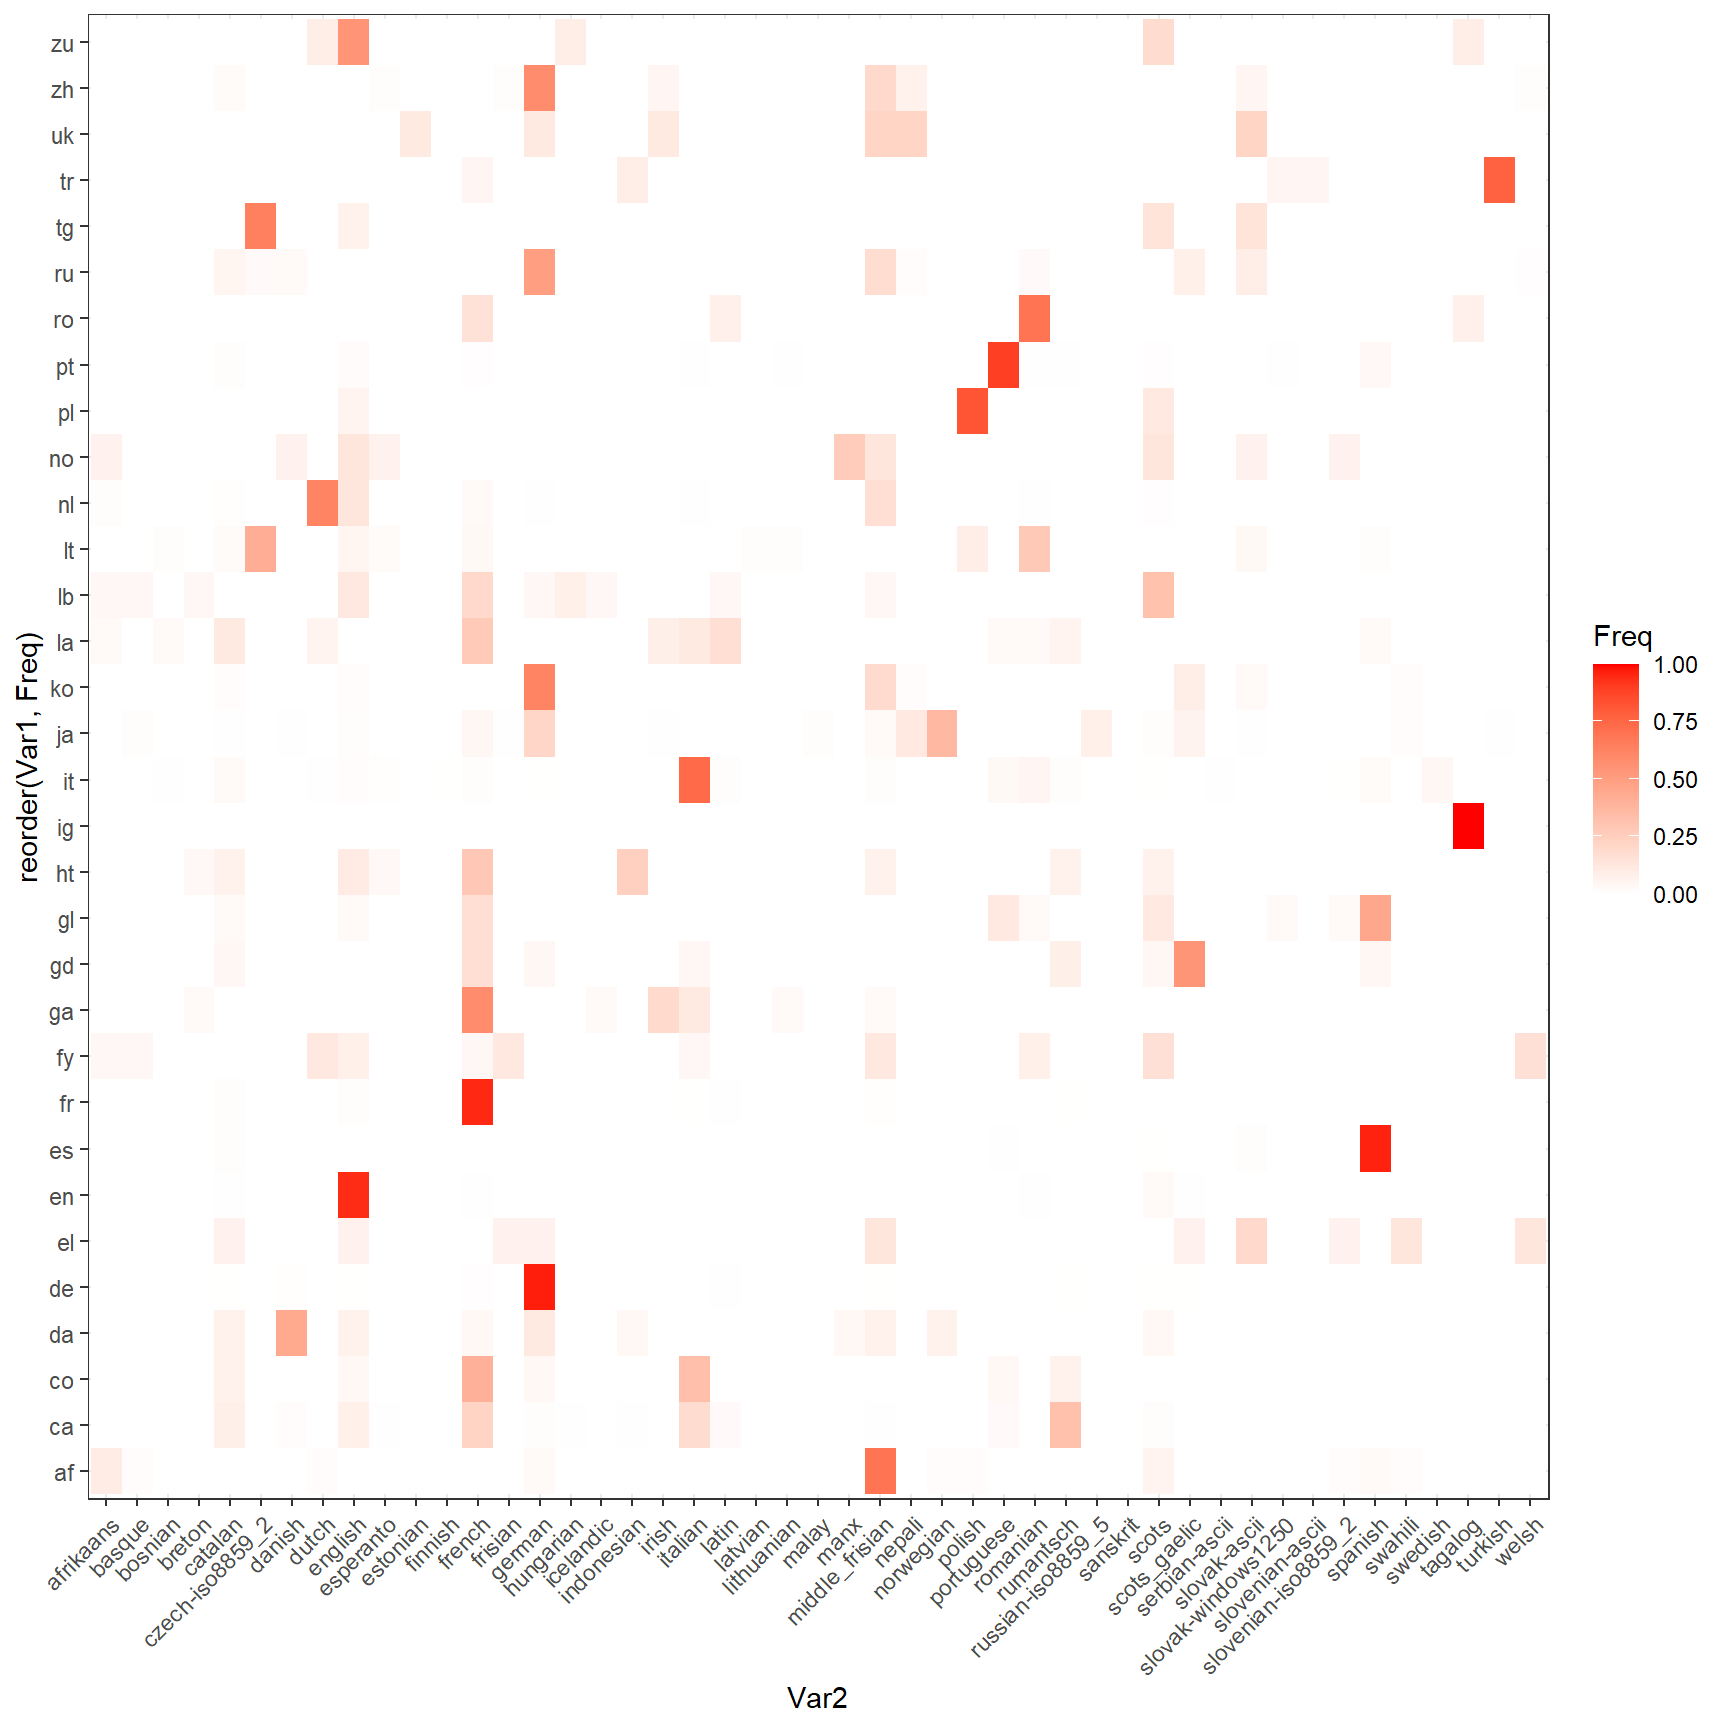
\includegraphics[width=0.8\linewidth]{bookdown-demo_files/figure-latex/303-2} 

}

\end{figure}

\begin{Shaded}
\begin{Highlighting}[]
\KeywordTok{library}\NormalTok{(pheatmap)}
\KeywordTok{library}\NormalTok{(viridis)}

\NormalTok{table2<-}\KeywordTok{as.data.frame}\NormalTok{(table) }\OperatorTok
\StringTok{  }\KeywordTok{mutate}\NormalTok{(}\DataTypeTok{Freq=}\KeywordTok{log10}\NormalTok{(Freq}\OperatorTok{+}\DecValTok{1}\NormalTok{))  }\OperatorTok\StringTok{ }
\StringTok{  }\KeywordTok{pivot_wider}\NormalTok{(}\DataTypeTok{names_from =}\NormalTok{ Var1, }\DataTypeTok{values_from =}\NormalTok{ Freq) }\OperatorTok
\StringTok{  }\KeywordTok{column_to_rownames}\NormalTok{( }\DataTypeTok{var =} \StringTok{"Var2"}\NormalTok{)}
\KeywordTok{pheatmap}\NormalTok{(table2 , }\DataTypeTok{color =} \KeywordTok{inferno}\NormalTok{(}\DecValTok{10}\NormalTok{))}
\end{Highlighting}
\end{Shaded}

\begin{figure}

{\centering 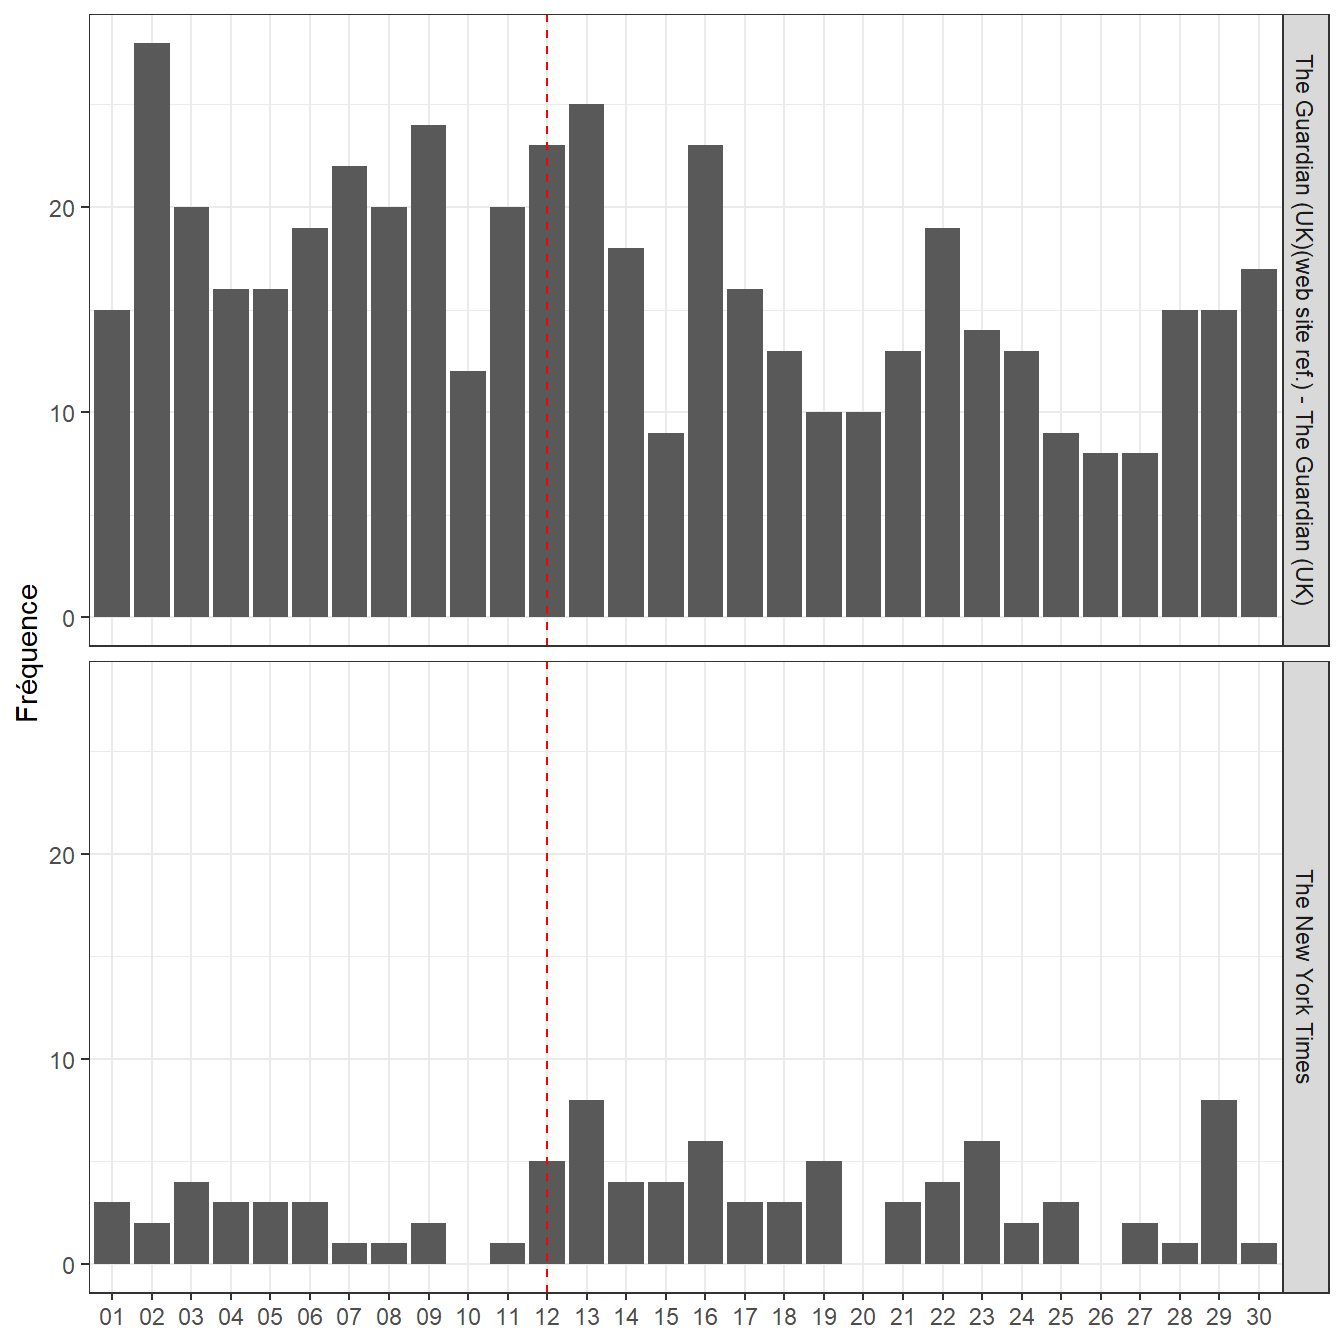
\includegraphics[width=0.8\linewidth]{bookdown-demo_files/figure-latex/304-1} 

}

\end{figure}

\begin{Shaded}
\begin{Highlighting}[]
\NormalTok{chi2<-}\StringTok{ }\KeywordTok{chisq.test}\NormalTok{(table)}
\NormalTok{chi2<-}\StringTok{ }\KeywordTok{as.data.frame}\NormalTok{(chi2}\OperatorTok{$}\NormalTok{residual)}

\NormalTok{table2<-chi2 }\OperatorTok\StringTok{ }\KeywordTok{mutate}\NormalTok{(}\DataTypeTok{Freq=}\NormalTok{Freq}\OperatorTok{^}\DecValTok{2}\NormalTok{)}\OperatorTok
\StringTok{  }\KeywordTok{pivot_wider}\NormalTok{(}\DataTypeTok{names_from =}\NormalTok{ Var1, }\DataTypeTok{values_from =}\NormalTok{ Freq) }\OperatorTok
\StringTok{  }\KeywordTok{column_to_rownames}\NormalTok{( }\DataTypeTok{var =} \StringTok{"Var2"}\NormalTok{)}
\KeywordTok{pheatmap}\NormalTok{(table2 , }\DataTypeTok{color =} \KeywordTok{inferno}\NormalTok{(}\DecValTok{20}\NormalTok{, }\DataTypeTok{direction=}\DecValTok{1}\NormalTok{))}
\end{Highlighting}
\end{Shaded}

\begin{figure}

{\centering 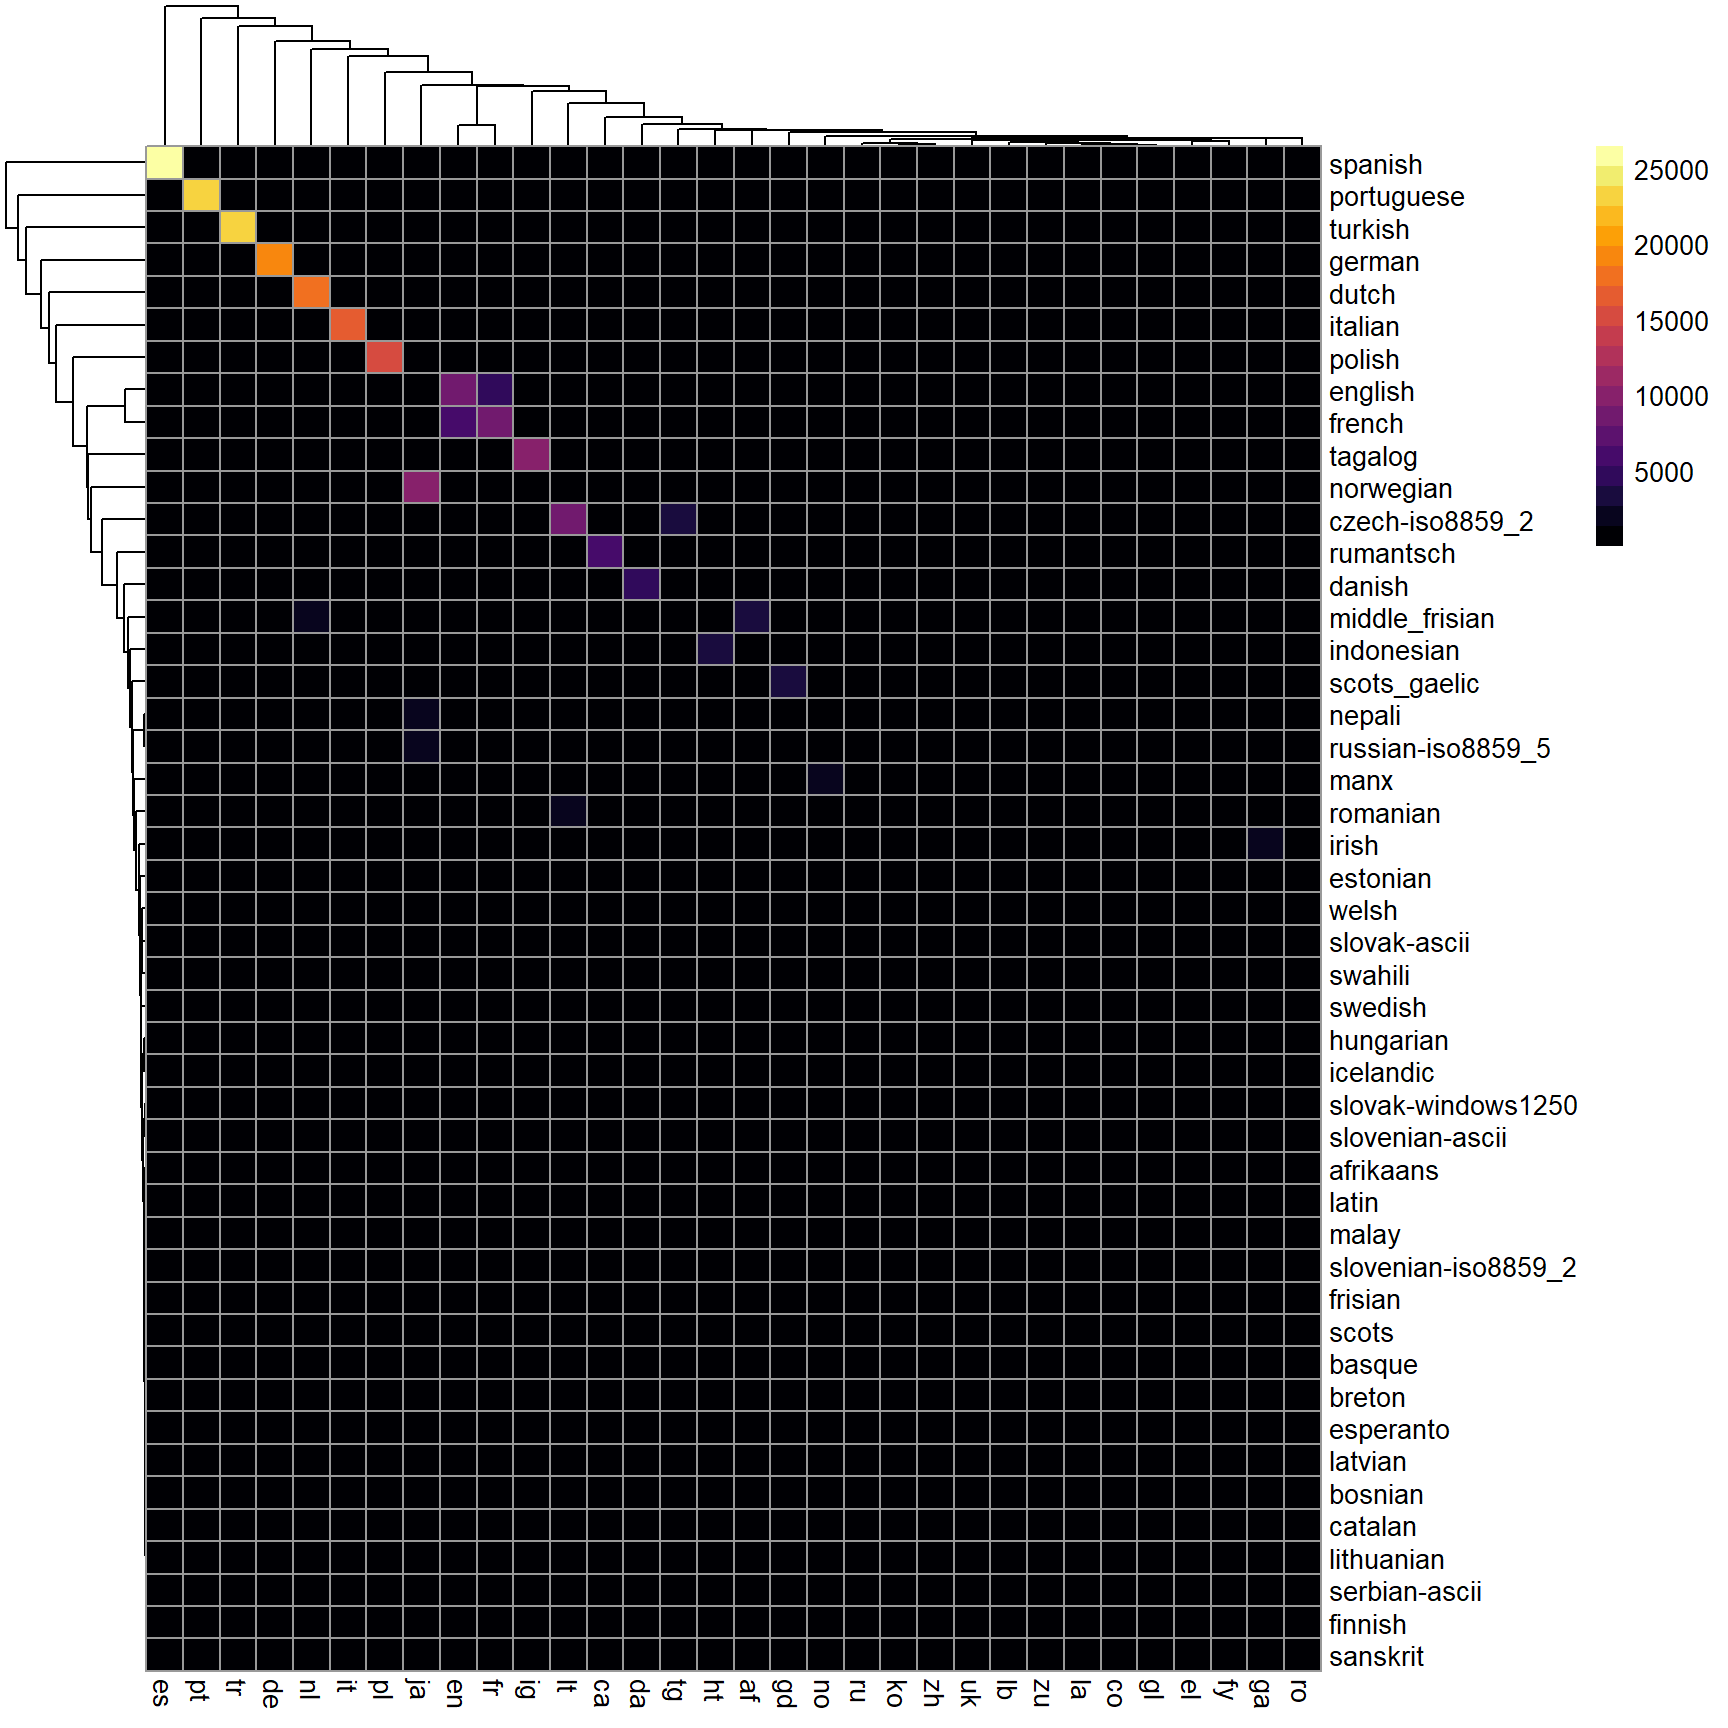
\includegraphics[width=0.8\linewidth]{bookdown-demo_files/figure-latex/304-2} 

}

\end{figure}

\hypertarget{identifier-les-plagiats-et-ruxe9utilisations}{%
\subsection{Identifier les plagiats et réutilisations}\label{identifier-les-plagiats-et-ruxe9utilisations}}

Dans la définition du corpus il peut être utile de se concentrer sur les contenus originaux

Une autre question est de detection les contenus riginaux des contenu réutilisés ou carrément plagiés.

\url{https://github.com/ropensci/textreuse}

\url{https://journal.r-project.org/archive/2020/RJ-2020-017/index.html}

\hypertarget{identifier-les-fakes}{%
\subsection{Identifier les fakes}\label{identifier-les-fakes}}

\url{https://github.com/sherylWM/Fake-News-Detection-using-Twitter}

\hypertarget{identifier-les-trolls}{%
\subsection{Identifier les trolls}\label{identifier-les-trolls}}

\url{http://golovchenko.github.io/tutorials/snatrolls}

\hypertarget{identifier-les-bots}{%
\subsection{Identifier les bots}\label{identifier-les-bots}}

botometer
botchecks

pour un benchmark

\url{https://rpubs.com/xil865/528096}

detecter les fakes \url{https://blogs.rstudio.com/ai/posts/2020-08-18-deepfake/}

\hypertarget{une-premiuxe8re-analyse-quantitative}{%
\chapter{Une première analyse quantitative}\label{une-premiuxe8re-analyse-quantitative}}

Avant tout un texte doit être analyser de manière volumétrique. Comment de texte? Quelle longueur ? combien de mots ? quelles variations?

Dans ce chapitre nous allons analyser le flux des tweets produit par donald Trump, jusqu'au moment de son banissement en Janvier 2021, àprès sa défaite.

Chargeons le fichier de données. On en profite pour compter le nombre de posts et de variables

\begin{Shaded}
\begin{Highlighting}[]
\NormalTok{df <-}\StringTok{ }\KeywordTok{read_csv}\NormalTok{(}\StringTok{"./data/TrumpTwitterArchive01-08-2021.csv"}\NormalTok{)}
\NormalTok{nrow<-}\KeywordTok{nrow}\NormalTok{(df) }\CommentTok{#nombre de ligne}
\NormalTok{ncol<-}\KeywordTok{ncol}\NormalTok{(df) }\CommentTok{#nombre de colonne}
\end{Highlighting}
\end{Shaded}

\hypertarget{comptons-les-mots}{%
\section{Comptons les mots}\label{comptons-les-mots}}

Il y 56571 tweets et 9 variables. On peut vouloir compter le nombre de mots. A cette fin on emploie une fonction de \texttt{stringr\ :}str\_count`. ( On reviendra sur la question de la manipulation des chaines de caractères dans un chapitre ad hoc)

\begin{Shaded}
\begin{Highlighting}[]
\NormalTok{df}\OperatorTok{$}\NormalTok{nb_mots<-}\KeywordTok{str_count}\NormalTok{(df}\OperatorTok{$}\NormalTok{text, }\StringTok{" "}\NormalTok{)}\OperatorTok{+}\DecValTok{1} \CommentTok{# l'astuce : compter les espaces et ajouter 1, pour compter les mots}
\NormalTok{sum_mots<-}\KeywordTok{sum}\NormalTok{(df}\OperatorTok{$}\NormalTok{nb_mots)             }\CommentTok{#ON COMPTE LE NOMBRE DE MOTS}
\KeywordTok{ggplot}\NormalTok{(df, }\KeywordTok{aes}\NormalTok{(}\DataTypeTok{x=}\NormalTok{nb_mots))}\OperatorTok{+}
\StringTok{  }\KeywordTok{geom_histogram}\NormalTok{(}\DataTypeTok{fill=}\StringTok{"deepskyblue3"}\NormalTok{)}\OperatorTok{+}
\StringTok{  }\KeywordTok{labs}\NormalTok{(}\DataTypeTok{title=}\KeywordTok{paste0}\NormalTok{(}\StringTok{"Nombre total de mots du corpus : "}\NormalTok{,sum_mots), }\DataTypeTok{x=}\StringTok{"Nombre de mots par post"}\NormalTok{, }\DataTypeTok{y=}\StringTok{"Fréquence"}\NormalTok{)}
\end{Highlighting}
\end{Shaded}

\begin{figure}

{\centering 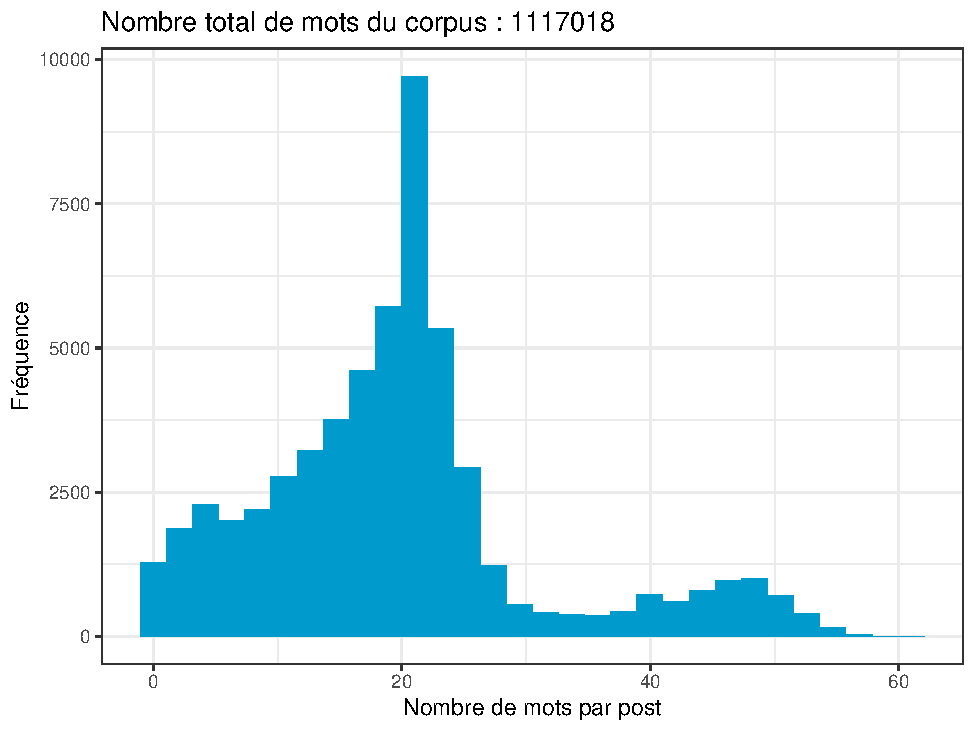
\includegraphics[width=0.8\linewidth]{bookdown-demo_files/figure-latex/1-1} 

}

\caption{Distribution du nombre de mots par post}\label{fig:1}
\end{figure}

La bimodalité provient surement du changement de taille maximum effectué en septembre 2017, le passage de 180 caractères max à 280. On peut le vérifier en examinant cette même distribution - par les courbes de densité - pour chacune des années, avec cette technique rendue fameuse par la pochette de l'album de Joy Division : un graphique en crêtes (ridges plot) avec \href{https://cran.r-project.org/web/packages/ggridges/vignettes/introduction.html}{ggridges}

\begin{Shaded}
\begin{Highlighting}[]
\NormalTok{df}\OperatorTok{$}\NormalTok{Year<-}\KeywordTok{format}\NormalTok{(df}\OperatorTok{$}\NormalTok{date, }\DataTypeTok{format =} \StringTok{"%Y"}\NormalTok{) }\CommentTok{#on extrait l'année de la date}

\KeywordTok{ggplot}\NormalTok{(df,}\KeywordTok{aes}\NormalTok{(}\DataTypeTok{x =}\NormalTok{ nb_mots, }\DataTypeTok{y =}\NormalTok{ Year, }\DataTypeTok{group =}\NormalTok{ Year)) }\OperatorTok{+}
\StringTok{  }\KeywordTok{geom_density_ridges}\NormalTok{(}\DataTypeTok{scale =} \DecValTok{3}\NormalTok{, }\DataTypeTok{fill=}\StringTok{"peachpuff"}\NormalTok{)}\OperatorTok{+}
\StringTok{  }\KeywordTok{theme_ridges}\NormalTok{() }\OperatorTok{+}
\StringTok{  }\KeywordTok{scale_x_continuous}\NormalTok{(}\DataTypeTok{limits =} \KeywordTok{c}\NormalTok{(}\DecValTok{1}\NormalTok{, }\DecValTok{70}\NormalTok{), }\DataTypeTok{expand =} \KeywordTok{c}\NormalTok{(}\DecValTok{0}\NormalTok{, }\DecValTok{0}\NormalTok{)) }\OperatorTok{+}
\StringTok{  }\KeywordTok{coord_cartesian}\NormalTok{(}\DataTypeTok{clip =} \StringTok{"off"}\NormalTok{)}\OperatorTok{+}\KeywordTok{labs}\NormalTok{(}\DataTypeTok{x=}\StringTok{"Nombre de mots par post"}\NormalTok{, }\DataTypeTok{y=}\OtherTok{NULL}\NormalTok{)}
\end{Highlighting}
\end{Shaded}

\begin{figure}

{\centering 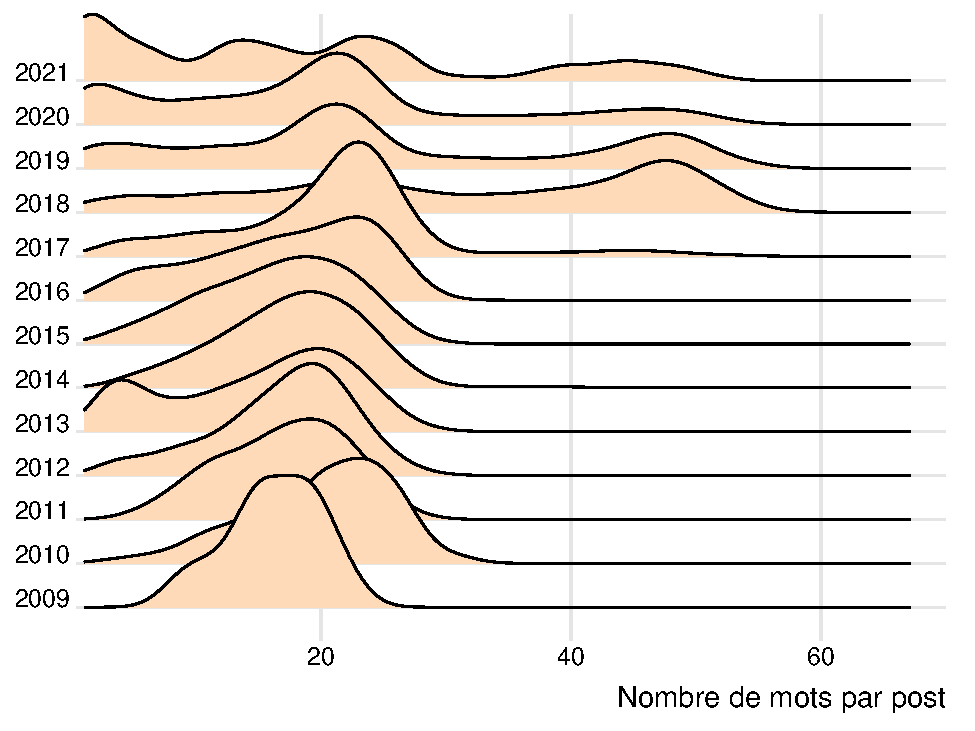
\includegraphics[width=0.8\linewidth]{bookdown-demo_files/figure-latex/2-1} 

}

\caption{ Evolution de la distribution du nombre de mots}\label{fig:2}
\end{figure}

\hypertarget{la-production-dans-le-temps}{%
\section{la production dans le temps}\label{la-production-dans-le-temps}}

Le résultat remarquable est que si Trump dans un premier temps exploite cette nouvel fonctionnalité, il en revient avec un phrasé de 20 mots en moyenne, gardant cependant à l'occasion d'autre contenu en 50 mots environ.

Concluons en examiner le nombre de tweets produit au cours du temps

\begin{Shaded}
\begin{Highlighting}[]
\CommentTok{## plot time series of tweets}
\KeywordTok{ts_plot}\NormalTok{(df, }\StringTok{"1 month"}\NormalTok{, }\DataTypeTok{color=}\StringTok{"darkblue"}\NormalTok{) }\OperatorTok{+}\StringTok{ }\KeywordTok{theme}\NormalTok{(}\DataTypeTok{plot.title =} \KeywordTok{element_text}\NormalTok{(}\DataTypeTok{face =} \StringTok{"bold"}\NormalTok{)) }\OperatorTok{+}\StringTok{ }
\StringTok{  }\KeywordTok{labs}\NormalTok{( }\DataTypeTok{x =} \OtherTok{NULL}\NormalTok{, }\DataTypeTok{y =} \StringTok{"Nombre de tweets par mois"}\NormalTok{,}\DataTypeTok{title =} \StringTok{"Fréquence des posts twitters Donald Trump"}\NormalTok{)}\OperatorTok{+}
\StringTok{  }\KeywordTok{scale_x_datetime}\NormalTok{(}\DataTypeTok{date_breaks =} \StringTok{"1 year"}\NormalTok{, }\DataTypeTok{labels =}\NormalTok{ scales}\OperatorTok{::}\KeywordTok{label_date_short}\NormalTok{())}
\end{Highlighting}
\end{Shaded}

\begin{figure}

{\centering 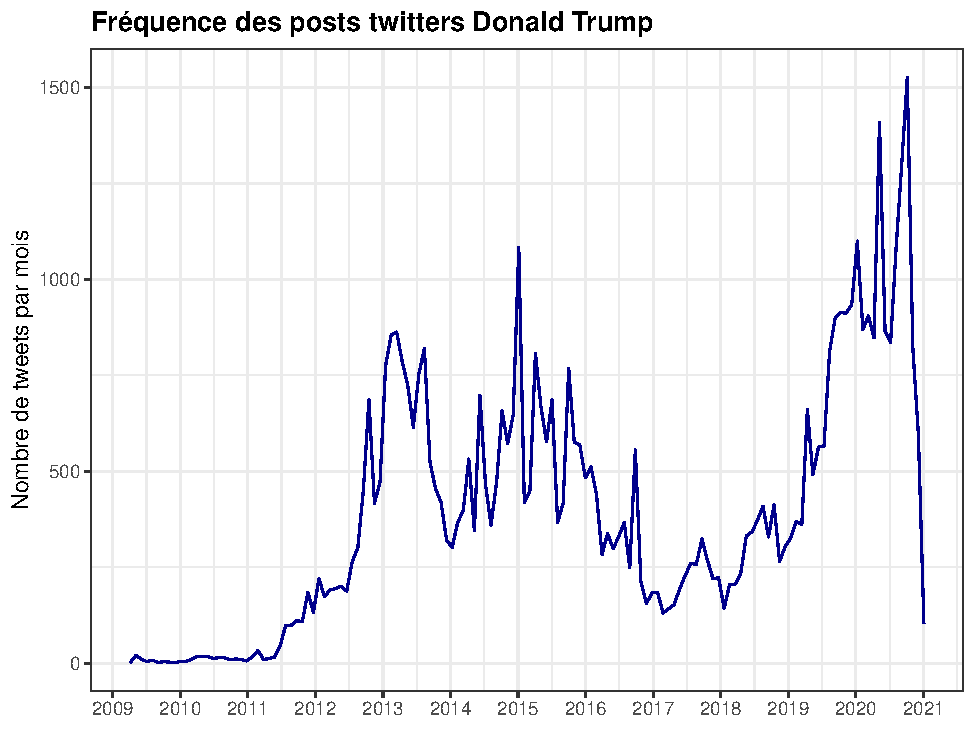
\includegraphics[width=0.8\linewidth]{bookdown-demo_files/figure-latex/3-1} 

}

\caption{Evolution de la production mensuelle des tweets de Trump}\label{fig:3}
\end{figure}

\begin{Shaded}
\begin{Highlighting}[]
\CommentTok{#raf : labeliser avec les dates clés}
\end{Highlighting}
\end{Shaded}

\hypertarget{lisibilituxe9-et-complexituxe9-lexicale}{%
\section{Lisibilité et complexité lexicale}\label{lisibilituxe9-et-complexituxe9-lexicale}}

Pour aller un peu plus loin, dans les comptages, introduisons deux quantifications utiles du texte : la lisibilité et la complexité lexicale. On gardera le principe d'une analyse longitudinale

\url{https://fr.wikipedia.org/wiki/Covfefe}

\hypertarget{les-indices-de-lisibilituxe9}{%
\subsection{Les indices de lisibilité}\label{les-indices-de-lisibilituxe9}}

La lisibilité est une vieille notion autant que sa mesure (par exemple \citet{coleman_computer_1975}). Il s'agit d'évaluer la complexité d'un texte à partir de deux critères : la complexité des mots capturée par le nombre moyen de syllabes par mot, et la complexité des phrases mesurée par le nombre de mots.

Le nombre d'indicateurs est considérable et le package compagnon de quanteda , \texttt{{[}quanteda.textstats{]}(https://quanteda.io/reference/textstat\_readability.html)} , en fournit au moins des dizaines. Dans l'exemple suivant, on se contente d'un grand classique, le plus ancien, l'indice de Flesch \citep{flesch_new_1948} et de ses constituants: le nombre moyen de syllabes par mot et le nombre moyen de mots par phrase.

\begin{Shaded}
\begin{Highlighting}[]
\NormalTok{foo<-df }\OperatorTok\StringTok{ }\KeywordTok{filter}\NormalTok{(isRetweet}\OperatorTok{==}\OtherTok{FALSE}\NormalTok{) }\CommentTok{# on ne prend pas en compte les RT}

\NormalTok{readability<-}\KeywordTok{textstat_readability}\NormalTok{(foo}\OperatorTok{$}\NormalTok{text, }\DataTypeTok{measure =} \KeywordTok{c}\NormalTok{(}\StringTok{"Flesch"}\NormalTok{,}\StringTok{"meanSentenceLength"}\NormalTok{, }\StringTok{"meanWordSyllables"}\NormalTok{),}
                                  \DataTypeTok{min_sentence_length =} \DecValTok{3}\NormalTok{,}\DataTypeTok{max_sentence_length =} \DecValTok{1000}\NormalTok{) }\CommentTok{#la fonction de calcul de lisibilité}

\NormalTok{foo<-}\KeywordTok{cbind}\NormalTok{(foo,readability[,}\DecValTok{2}\OperatorTok{:}\DecValTok{4}\NormalTok{])}
\NormalTok{foo1<-foo }\OperatorTok\StringTok{ }
\StringTok{  }\KeywordTok{group_by}\NormalTok{(Year) }\OperatorTok
\StringTok{  }\KeywordTok{summarise}\NormalTok{(}\DataTypeTok{Flesch=}\KeywordTok{mean}\NormalTok{(Flesch, }\DataTypeTok{na.rm=}\OtherTok{TRUE}\NormalTok{), }
            \DataTypeTok{SentenceLength=} \KeywordTok{mean}\NormalTok{(meanSentenceLength, }\DataTypeTok{na.rm=}\OtherTok{TRUE}\NormalTok{),}
            \DataTypeTok{WordSyllables=} \KeywordTok{mean}\NormalTok{(meanWordSyllables, }\DataTypeTok{na.rm=}\OtherTok{TRUE}\NormalTok{)) }\OperatorTok
\StringTok{  }\KeywordTok{gather}\NormalTok{(variable, value, }\OperatorTok{-}\NormalTok{Year)}

\KeywordTok{ggplot}\NormalTok{(foo1,}\KeywordTok{aes}\NormalTok{(}\DataTypeTok{x=}\NormalTok{Year, }\DataTypeTok{y=}\NormalTok{value, }\DataTypeTok{group=}\NormalTok{variable))}\OperatorTok{+}
\StringTok{  }\KeywordTok{geom_line}\NormalTok{(}\DataTypeTok{size=}\FloatTok{1.2}\NormalTok{, }\KeywordTok{aes}\NormalTok{(}\DataTypeTok{color=}\NormalTok{variable), }\DataTypeTok{stat=}\StringTok{"identity"}\NormalTok{)}\OperatorTok{+}
\StringTok{  }\KeywordTok{facet_wrap}\NormalTok{(}\KeywordTok{vars}\NormalTok{(variable), }\DataTypeTok{scale=}\StringTok{"free"}\NormalTok{, }\DataTypeTok{ncol=}\DecValTok{1}\NormalTok{)}\OperatorTok{+}
\StringTok{  }\KeywordTok{labs}\NormalTok{(}\DataTypeTok{title =} \StringTok{"Evolution de la lisibilité des tweets de Trump"}\NormalTok{, }\DataTypeTok{x=}\OtherTok{NULL}\NormalTok{, }\DataTypeTok{y=}\OtherTok{NULL}\NormalTok{)}
\end{Highlighting}
\end{Shaded}

\begin{figure}

{\centering 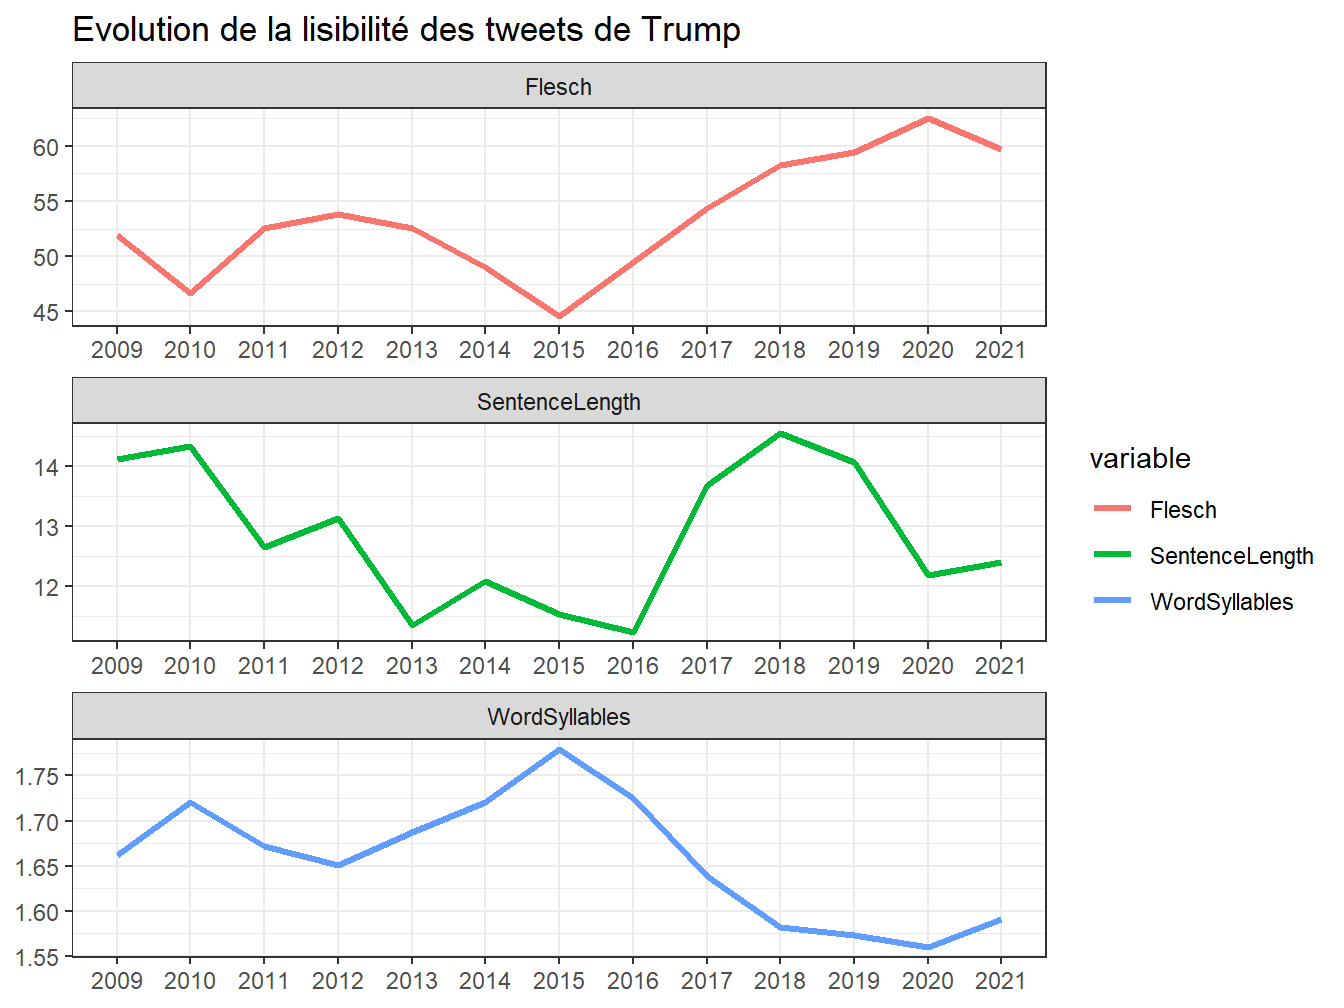
\includegraphics[width=0.8\linewidth]{bookdown-demo_files/figure-latex/404-1} 

}

\caption{Evolution de la lisibilité moyenne des tweets de Trump}\label{fig:404}
\end{figure}

Pour aider le lecteur à donner un sens, voici l'abaque proposée par \href{http://www.appstate.edu/~steelekm/classes/psy2664/Flesch.htm}{Flesch}lui-même. \href{ReadabilityFlesch.JPG}{Flesch}. On peut aussi prendre pour références les éléments suivants: ``All Plain English examples in this book score at least 60. Here are the scores of some reading materials I've tested. These are average scores of random samples.''

Comics 92
Consumer ads in magazines 82
Reader's Digest 65
Time 52
Wall Street Journal 43
Harvard Business Review 43
Harvard Law Review 32
Auto insurance policy 10

Trump ne parait pas être sa caricature, non niveau de lisibilité correspond à la Licence. Il est moins simple que le Reader's Digest mais plus compliqué à lire que la Harvard Business Review !

\hypertarget{les-indices-de-complexituxe9-lexicale}{%
\subsection{Les indices de complexité lexicale}\label{les-indices-de-complexituxe9-lexicale}}

La complexité lexicale rend compte de la diversité du vocabulaire, elle consiste à rapporter le nombre de mot uniques sur le nombre total de mots. La difficulté est que la taille des corpus joue fortement sur cette mesure et que l'orsque cette taille est hétérogène, l'indicateur marque plus cette variété que les variations de complexité lexicale.\citep{tweedie_how_1998}

\url{https://quanteda.io/reference/textstat_lexdiv.html}

Une manière plus fine sera de considérer chaque période comme un texte,

un pb est que l'allongement des tweets peut expliquer l'accroissement de diversité

Dans notre univers trumpesque, ce n'est pas trop sensible, d'autant plus que nous allons moyenner les tweets par période.Notons au passage que si nous moyennons la diversité lexicale de chaque tweets , une autre approche pourrait être de concatener l'ensemble des tweets d'une période ( un jour, une semaine) pour approcher cette variable à une autre échelle, qui couvrent l'ensemble des sujets d'intérêt de trump, que les tweets fractionnenet nécessairement. Ce qui en en question dans la mise en pratique n'est pas seulement la question du choix de l'indice mais aussi la définition de l'unité de calcul. La diversité lexical concerne sans doute plus le discours que la phrase.

là, encore la nécessité d'avoir des points de repère, des échelles.

\begin{Shaded}
\begin{Highlighting}[]
\NormalTok{lexdiv<-}\KeywordTok{tokens}\NormalTok{(foo}\OperatorTok{$}\NormalTok{text) }\OperatorTok\StringTok{ }
\StringTok{  }\KeywordTok{textstat_lexdiv}\NormalTok{(foo}\OperatorTok{$}\NormalTok{text, }\DataTypeTok{measure =} \KeywordTok{c}\NormalTok{(}\StringTok{"CTTR"}\NormalTok{),}\DataTypeTok{remove_numbers =} \OtherTok{TRUE}\NormalTok{,}
  \DataTypeTok{remove_punct =} \OtherTok{TRUE}\NormalTok{,}
  \DataTypeTok{remove_symbols =} \OtherTok{TRUE}\NormalTok{,}
  \DataTypeTok{remove_hyphens =} \OtherTok{FALSE}\NormalTok{) }\CommentTok{#la fonction de calcul de diversité}

\NormalTok{foo<-}\KeywordTok{cbind}\NormalTok{(foo,lexdiv[,}\DecValTok{2}\NormalTok{])}
\NormalTok{foo1<-foo }\OperatorTok\StringTok{ }
\StringTok{  }\KeywordTok{group_by}\NormalTok{(Year) }\OperatorTok
\StringTok{  }\KeywordTok{summarise}\NormalTok{(}\DataTypeTok{CTTR=}\KeywordTok{mean}\NormalTok{(CTTR, }\DataTypeTok{na.rm=}\OtherTok{TRUE}\NormalTok{)) }\OperatorTok
\StringTok{  }\KeywordTok{gather}\NormalTok{(variable, value, }\OperatorTok{-}\NormalTok{Year)}

\KeywordTok{ggplot}\NormalTok{(foo1,}\KeywordTok{aes}\NormalTok{(}\DataTypeTok{x=}\NormalTok{Year, }\DataTypeTok{y=}\NormalTok{value, }\DataTypeTok{group=}\NormalTok{variable))}\OperatorTok{+}
\StringTok{  }\KeywordTok{geom_line}\NormalTok{(}\DataTypeTok{size=}\FloatTok{1.2}\NormalTok{, }\KeywordTok{aes}\NormalTok{(}\DataTypeTok{color=}\NormalTok{variable), }\DataTypeTok{stat=}\StringTok{"identity"}\NormalTok{)}\OperatorTok{+}
\StringTok{  }\KeywordTok{facet_wrap}\NormalTok{(}\KeywordTok{vars}\NormalTok{(variable), }\DataTypeTok{scale=}\StringTok{"free"}\NormalTok{, }\DataTypeTok{ncol=}\DecValTok{1}\NormalTok{)}\OperatorTok{+}
\StringTok{  }\KeywordTok{labs}\NormalTok{(}\DataTypeTok{title =} \StringTok{"Evolution de la diversité lexicale des tweets de Trump"}\NormalTok{, }\DataTypeTok{x=}\OtherTok{NULL}\NormalTok{, }\DataTypeTok{y=}\OtherTok{NULL}\NormalTok{)}
\end{Highlighting}
\end{Shaded}

\begin{figure}

{\centering 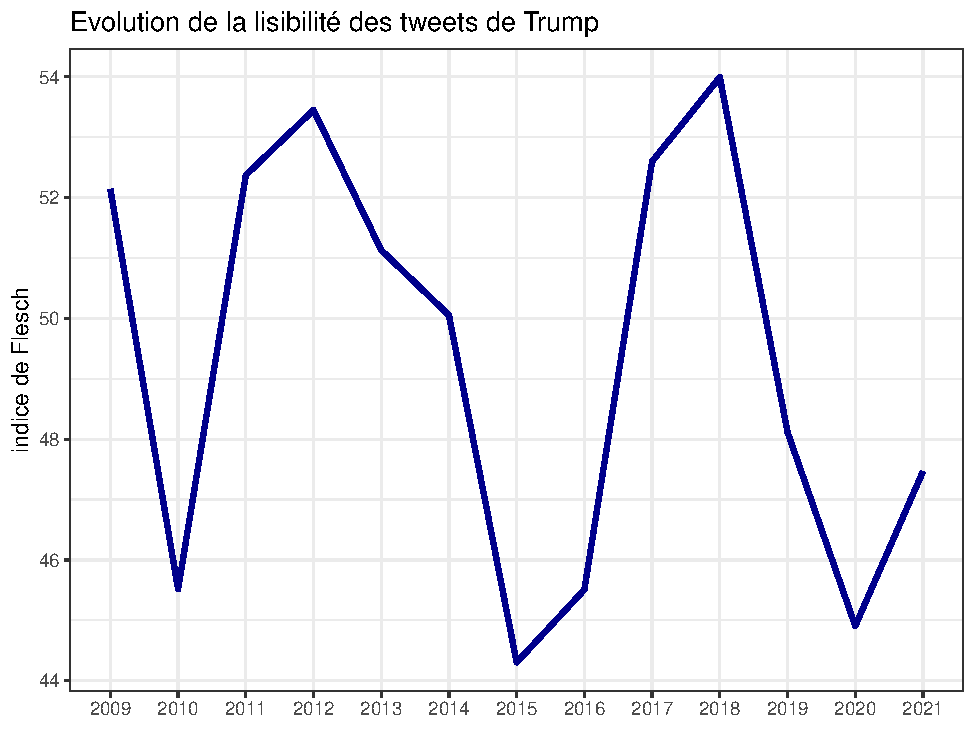
\includegraphics[width=0.8\linewidth]{bookdown-demo_files/figure-latex/4-1} 

}

\caption{Evolution de la lisibilité moyenne des tweets de Trump}\label{fig:4}
\end{figure}

\hypertarget{conclusion-2}{%
\section{Conclusion}\label{conclusion-2}}

Nous aurons appris à

\begin{itemize}
\tightlist
\item
  compter le nombre de document
\item
  mesurer la complexité du langage
\item
  mesurer la diversité de son vocabulaire.
\end{itemize}

Ces mesures n'ont ne sens que si elles peuvent être comparées

de manière interne

de manière externe

\hypertarget{token}{%
\chapter{Tokenisation}\label{token}}

\hypertarget{objectifs-du-chapitre}{%
\section{\texorpdfstring{\emph{Objectifs du chapitre}}{Objectifs du chapitre}}\label{objectifs-du-chapitre}}

\begin{itemize}
\tightlist
\item
  Découper un texte en \emph{tokens}
\item
  Visualiser les n-grammes du texte
\item
  Identifier les n-grammes pertinents et les transformer en \emph{tokens}
\end{itemize}

\hypertarget{les-outils}{%
\section{Les outils}\label{les-outils}}

\begin{itemize}
\tightlist
\item
  Jeu de données : une citation de Max Weber et le corpus des commentaires laissés sur TripAdvisor concernant les hôtels polynésiens.
\item
  Packages utilisés : \href{https://cran.r-project.org/web/packages/tokenizers/vignettes/introduction-to-tokenizers.html}{\texttt{tokenizer}} ; \href{https://quanteda.io}{\texttt{quanteda}} ; \href{https://github.com/quanteda/stopwords}{`stopwords'}
\end{itemize}

\hypertarget{introduction}{%
\section{Introduction}\label{introduction}}

L'étape intiale de toute analyse textuelle est de découper le texte en unités d'analyse, les \emph{tokens}, ce qui transforme le texte écrit pour la compréhension humaine en données interprétables par l'ordinateur. Les \emph{tokens} utilisés peuvent varier selon les objectifs de l'analyse et la nature du corpus, la granularité peut être plus ou moins fine. Les \emph{tokens} peuvent ainsi être :

\begin{itemize}
\tightlist
\item
  des lettres : c'est l'unité insécable
\item
  des syllabes : ça permet de s'intéresser aux phonèmes
\item
  des mots : il s'agit du niveau le plus évident et le plus courant, que l'on privilégiera tout au long de ce livre
\item
  des phrases : c'est l'unité de langage, lui correpond un argument, une proposition ; l'usage du point suivi d'un espace et d'une majuscule est assez général pour les identifier
\item
  des paragraphes : c'est une unité plus générale, qui souvent développe une idée
\item
  des sections, des chapitres, ou des livres : selon la nature des documents, cela permet de découper le corpus en sous-unités.
\end{itemize}

Les \emph{tokenizers} sont les outils indispensables à cette tâche. Dans cet ouvrage, nous nous concentrons sur l'étude des mots. Lors de cette étude, un certain nombre de mots apparaissent de nombreuses fois, pour permettre de donner du sens au langage humain, mais ils ne portent pas en eux d'informations particulièrement pertinentes pour l'analyse : ce sont les \emph{stopwords}, qu'il conviendra souvent d'éliminer.

Les n-grammes, quant à eux, représentent des suites de n \emph{tokens}. Un unigramme est donc équivalent à un \emph{token}, un bigramme est une suite de deux \emph{tokens}, etc. L'identification des n-grammes permet de détecter des suites de \emph{tokens} qui reviennent plus souvent que leur probabilité d'occurrences. Si l'on se concentre sur les mots, nous sommes alors face à une unité sémantique, comme on le comprend facilement avec le bigramme `Assemblée Nationale'.

\hypertarget{tokeniser-un-corpus}{%
\section{Tokeniser un corpus}\label{tokeniser-un-corpus}}

\hypertarget{les-lettres}{%
\subsection{Les lettres}\label{les-lettres}}

Commençons par un exemple simple, à l'aide d'une courte citation de Max Weber. On choisit les lettres pour unité de découpe, et l'on utilise le package `tokenizer'. Automatiquement, `tokenizer' met le texte en minuscule et élimine la ponctuation

\begin{Shaded}
\begin{Highlighting}[]
\CommentTok{#Les données}
\NormalTok{MaxWeber <-}\StringTok{ }\KeywordTok{paste0}\NormalTok{(}\StringTok{"Bureaucratie: le moyen le plus rationnel que l’on connaisse pour exercer un contrôle impératif sur des êtres humains."}\NormalTok{)}

\CommentTok{#On tokenise, plus on transforme en dataframe le résultat.}
\NormalTok{toc_maxweber<-}\KeywordTok{tokenize_characters}\NormalTok{(MaxWeber)}\OperatorTok
\StringTok{        }\KeywordTok{as.data.frame}\NormalTok{()}\OperatorTok
\StringTok{        }\KeywordTok{rename}\NormalTok{(}\DataTypeTok{tokens=}\DecValTok{1}\NormalTok{)}
\CommentTok{#On compte pour chaque token sa fréquence d'apparition}
\NormalTok{foo<-toc_maxweber }\OperatorTok\KeywordTok{mutate}\NormalTok{(}\DataTypeTok{n=}\DecValTok{1}\NormalTok{) }\OperatorTok\StringTok{ }
\StringTok{        }\KeywordTok{group_by}\NormalTok{(tokens)}\OperatorTok\StringTok{ }
\StringTok{        }\KeywordTok{summarise}\NormalTok{(}\DataTypeTok{n=}\KeywordTok{sum}\NormalTok{(n))}\OperatorTok\KeywordTok{filter}\NormalTok{(n}\OperatorTok{>}\DecValTok{0}\NormalTok{)}
\CommentTok{#On représente par un diagramme en barre cette distribution des occuences d'apparition, en classant les tokens par fréquence}
\KeywordTok{ggplot}\NormalTok{(foo, }\KeywordTok{aes}\NormalTok{(}\DataTypeTok{x=}\KeywordTok{reorder}\NormalTok{(tokens,n), }\DataTypeTok{y=}\NormalTok{n))}\OperatorTok{+}
\StringTok{               }\KeywordTok{geom_bar}\NormalTok{(}\DataTypeTok{stat=}\StringTok{"identity"}\NormalTok{, }\DataTypeTok{fill=}\StringTok{"royalblue"}\NormalTok{)}\OperatorTok{+}
\StringTok{        }\KeywordTok{annotate}\NormalTok{(}\StringTok{"text"}\NormalTok{, }\DataTypeTok{x=}\DecValTok{10}\NormalTok{,}\DataTypeTok{y=}\DecValTok{10}\NormalTok{, }\DataTypeTok{label=}\KeywordTok{paste}\NormalTok{(}\StringTok{"nombre de tokens ="}\NormalTok{, }\KeywordTok{nrow}\NormalTok{(toc_maxweber)))}\OperatorTok{+}
\StringTok{               }\KeywordTok{coord_flip}\NormalTok{()}\OperatorTok{+}\KeywordTok{labs}\NormalTok{(}\DataTypeTok{title =} \StringTok{"Fréquence des tokens, unité = lettres"}\NormalTok{, }\DataTypeTok{x=}\StringTok{"tokens"}\NormalTok{, }\DataTypeTok{y=}\StringTok{"nombre d'occurences"}\NormalTok{, }\DataTypeTok{caption =}\StringTok{" 'Bureaucratie: le moyen le plus rationnel que l’on connaisse pour exercer un contrôle impératif sur des êtres humains.' "}\NormalTok{)}
\end{Highlighting}
\end{Shaded}

\begin{figure}

{\centering 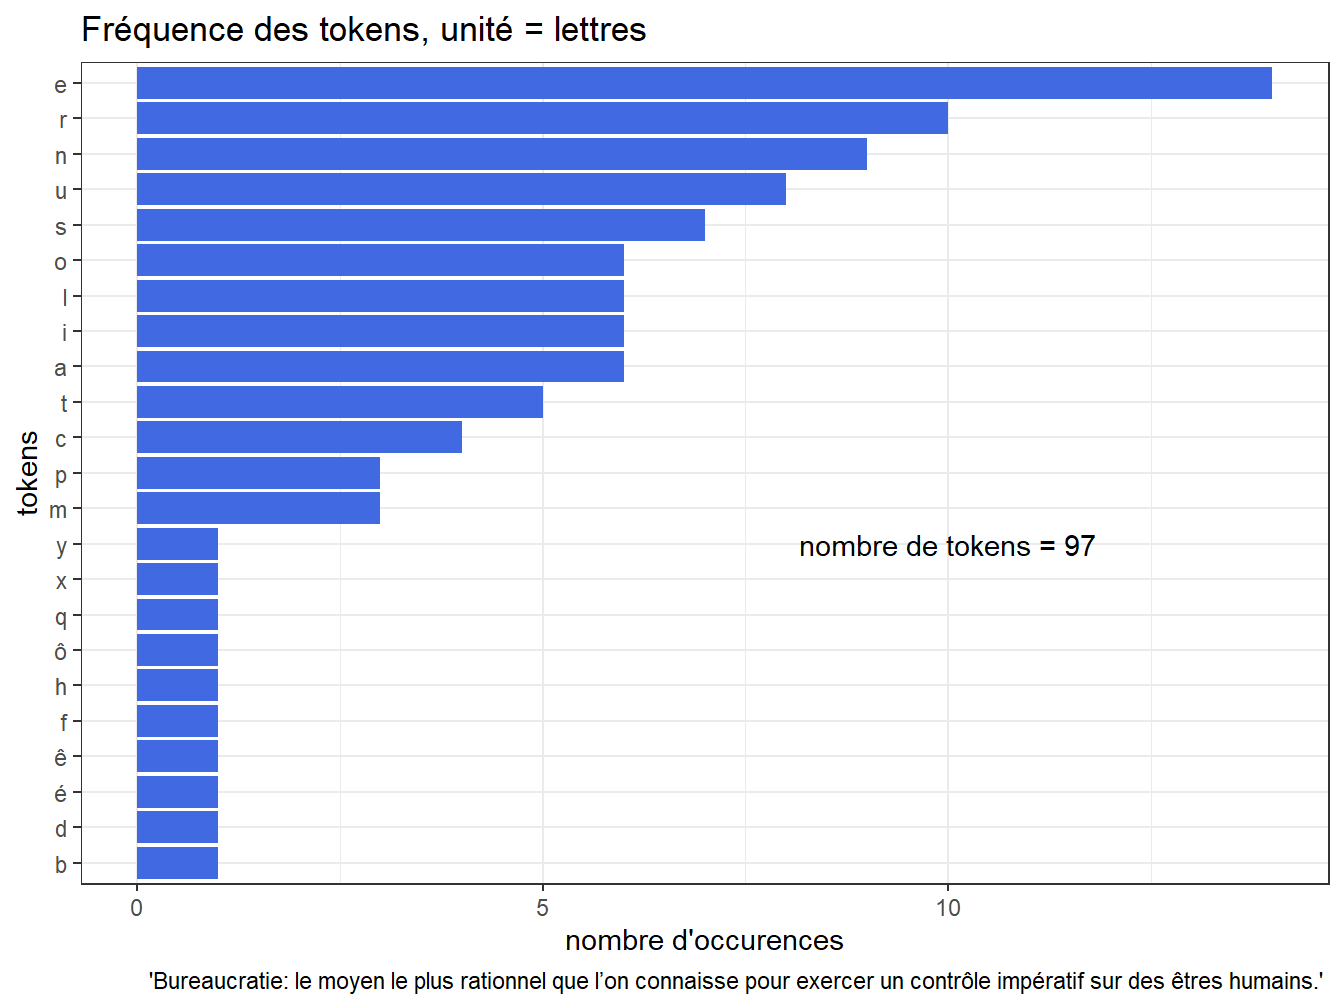
\includegraphics[width=0.8\linewidth]{bookdown-demo_files/figure-latex/501-1} 

}

\caption{Distribution du nombre de lettres}\label{fig:501}
\end{figure}

\hypertarget{les-mots}{%
\subsection{Les mots}\label{les-mots}}

On refait la même opération, mais avec un texte complété. Il y a bien moins de mots que de lettres !

\begin{Shaded}
\begin{Highlighting}[]
\CommentTok{#Les données}

\NormalTok{MaxWeber <-}\StringTok{ }\KeywordTok{paste0}\NormalTok{(}\StringTok{"Bureaucratie: le moyen le plus rationnel que l’on connaisse pour exercer un contrôle impératif sur des êtres humains. La bureaucratie est une forme d'organisation générale caractérisée par la prépondérance des règles et de procédures qui sont appliquées de façon impersonnelle par des agents spécialisés. Ces agents appliquent les règles sans discuter des objectifs ou des raisons qui les fondent. Ils doivent faire preuve de neutralité et oublier leurs propres intérêts personnels au profit de l’intérêt général."}\NormalTok{)}

\CommentTok{#On tokenise, plus on transforme en dataframe le résultat.}
\NormalTok{toc_maxweber<-}\KeywordTok{tokenize_words}\NormalTok{(MaxWeber)}\OperatorTok
\StringTok{        }\KeywordTok{as.data.frame}\NormalTok{()}\OperatorTok
\StringTok{        }\KeywordTok{rename}\NormalTok{(}\DataTypeTok{tokens=}\DecValTok{1}\NormalTok{)}

\CommentTok{#On compte pour chaque token sa fréquence d'apparition}
\NormalTok{foo<-toc_maxweber }\OperatorTok\KeywordTok{mutate}\NormalTok{(}\DataTypeTok{n=}\DecValTok{1}\NormalTok{) }\OperatorTok\StringTok{ }
\StringTok{        }\KeywordTok{group_by}\NormalTok{(tokens)}\OperatorTok\StringTok{ }
\StringTok{        }\KeywordTok{summarise}\NormalTok{(}\DataTypeTok{n=}\KeywordTok{sum}\NormalTok{(n))}

\CommentTok{#On représente par un diagramme en barre cette distribution des occurrences, en classant les tokens par fréquence}
\KeywordTok{ggplot}\NormalTok{(foo, }\KeywordTok{aes}\NormalTok{(}\DataTypeTok{x=}\KeywordTok{reorder}\NormalTok{(tokens,n), }\DataTypeTok{y=}\NormalTok{n))}\OperatorTok{+}
\StringTok{               }\KeywordTok{geom_bar}\NormalTok{(}\DataTypeTok{stat=}\StringTok{"identity"}\NormalTok{, }\DataTypeTok{fill=}\StringTok{"royalblue"}\NormalTok{)}\OperatorTok{+}
\StringTok{        }\KeywordTok{annotate}\NormalTok{(}\StringTok{"text"}\NormalTok{, }\DataTypeTok{x=}\DecValTok{10}\NormalTok{,}\DataTypeTok{y=}\DecValTok{4}\NormalTok{, }\DataTypeTok{label=}\KeywordTok{paste}\NormalTok{(}\StringTok{"nombre de tokens ="}\NormalTok{, }\KeywordTok{nrow}\NormalTok{(toc_maxweber)))}\OperatorTok{+}
\StringTok{               }\KeywordTok{coord_flip}\NormalTok{()}\OperatorTok{+}\KeywordTok{labs}\NormalTok{(}\DataTypeTok{title =} \StringTok{"Fréquence des tokens, unité = mots"}\NormalTok{, }\DataTypeTok{x=}\StringTok{"tokens"}\NormalTok{, }\DataTypeTok{y=}\StringTok{"nombre d'occurences"}\NormalTok{, }\DataTypeTok{caption =}\StringTok{" 'Bureaucratie: le moyen le plus rationnel que l’on connaisse pour exercer un contrôle impératif sur des êtres humains.' "}\NormalTok{)}
\end{Highlighting}
\end{Shaded}

\begin{figure}

{\centering 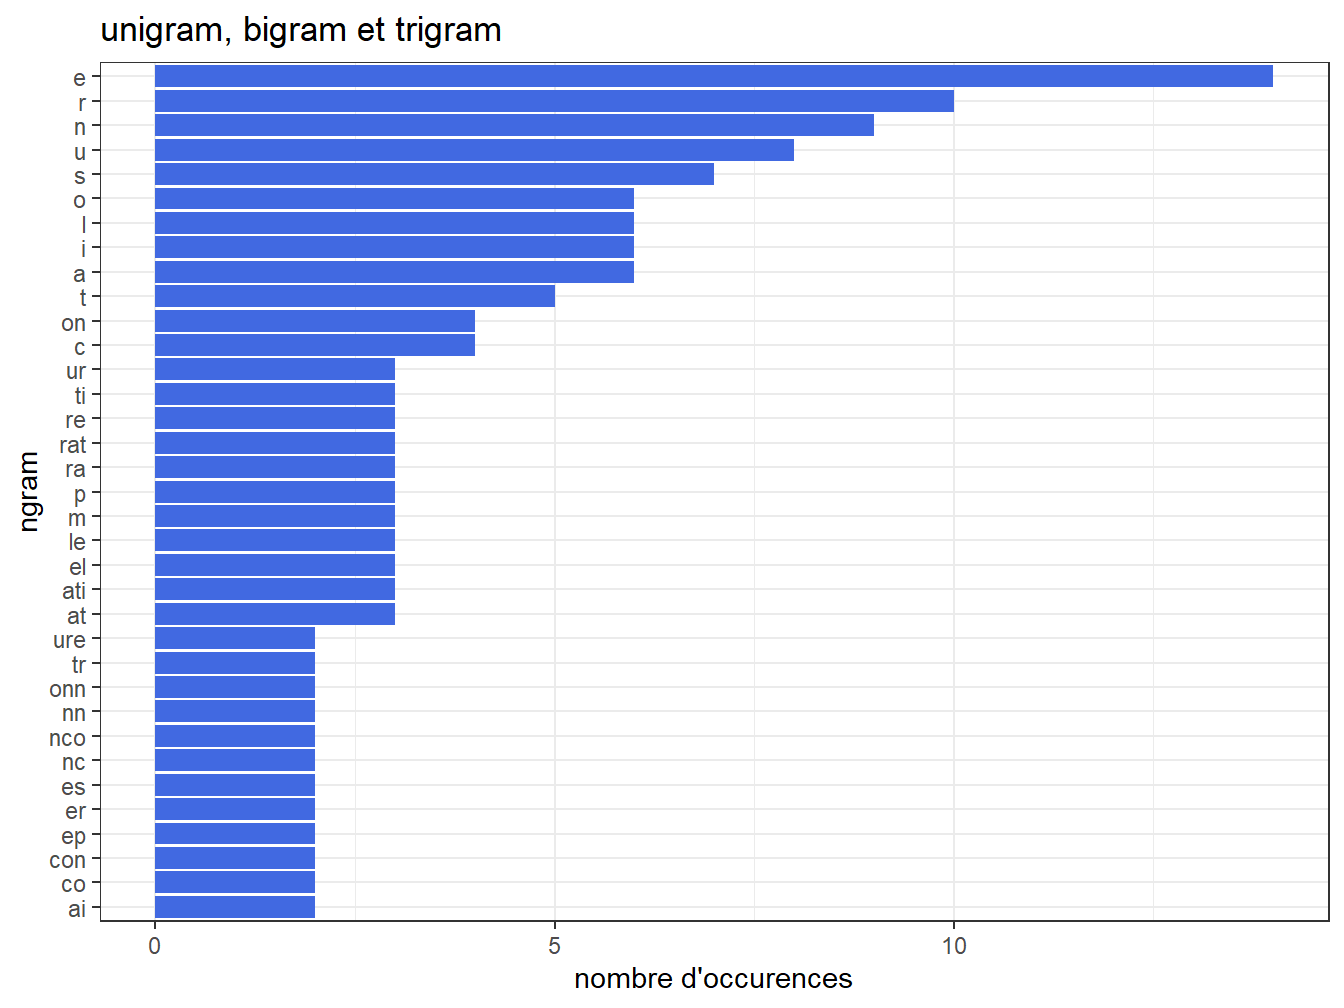
\includegraphics[width=0.8\linewidth]{bookdown-demo_files/figure-latex/502-1} 

}

\caption{Distribution du nombre de mots}\label{fig:502}
\end{figure}

On constate que les deux mots les plus fréquents de cette citation sont un article indéfini et une préposition. Ces mots sont souvent superflus pour les analyses menées, il convient alors de les supprimer. C'est ce qu'on fait par la suite, en utilisant le package `stopwords' qui comprend des listes de stopwords dans différentes langues.

\begin{Shaded}
\begin{Highlighting}[]
\CommentTok{#On tokenise et on enlève les stopwords, puis on transforme en dataframe le résultat.}
\NormalTok{toc_maxweber<-}\KeywordTok{tokenize_words}\NormalTok{(MaxWeber, }\DataTypeTok{stopwords =} \KeywordTok{stopwords}\NormalTok{(}\StringTok{"fr"}\NormalTok{))}\OperatorTok
\StringTok{        }\KeywordTok{as.data.frame}\NormalTok{()}\OperatorTok
\StringTok{        }\KeywordTok{rename}\NormalTok{(}\DataTypeTok{tokens=}\DecValTok{1}\NormalTok{)}

\CommentTok{#On compte pour chaque token sa fréquence d'apparition}
\NormalTok{foo<-toc_maxweber }\OperatorTok\KeywordTok{mutate}\NormalTok{(}\DataTypeTok{n=}\DecValTok{1}\NormalTok{) }\OperatorTok\StringTok{ }
\StringTok{        }\KeywordTok{group_by}\NormalTok{(tokens)}\OperatorTok\StringTok{ }
\StringTok{        }\KeywordTok{summarise}\NormalTok{(}\DataTypeTok{n=}\KeywordTok{sum}\NormalTok{(n))}\OperatorTok\KeywordTok{filter}\NormalTok{(n}\OperatorTok{>}\DecValTok{0}\NormalTok{)}

\CommentTok{#On représente par un diagramme en barre cette distribution des occurrences, en classant les tokens par fréquence}
\KeywordTok{ggplot}\NormalTok{(foo, }\KeywordTok{aes}\NormalTok{(}\DataTypeTok{x=}\KeywordTok{reorder}\NormalTok{(tokens,n), }\DataTypeTok{y=}\NormalTok{n))}\OperatorTok{+}
\StringTok{               }\KeywordTok{geom_bar}\NormalTok{(}\DataTypeTok{stat=}\StringTok{"identity"}\NormalTok{, }\DataTypeTok{fill=}\StringTok{"royalblue"}\NormalTok{)}\OperatorTok{+}
\StringTok{        }\KeywordTok{annotate}\NormalTok{(}\StringTok{"text"}\NormalTok{, }\DataTypeTok{x=}\DecValTok{10}\NormalTok{,}\DataTypeTok{y=}\FloatTok{1.5}\NormalTok{, }\DataTypeTok{label=}\KeywordTok{paste}\NormalTok{(}\StringTok{"nombre de tokens ="}\NormalTok{, }\KeywordTok{nrow}\NormalTok{(toc_maxweber)))}\OperatorTok{+}
\StringTok{               }\KeywordTok{coord_flip}\NormalTok{()}\OperatorTok{+}\KeywordTok{labs}\NormalTok{(}\DataTypeTok{title =} \StringTok{"Fréquence des tokens, unité = mots, stopwords éliminés"}\NormalTok{, }\DataTypeTok{x=}\StringTok{"tokens"}\NormalTok{, }\DataTypeTok{y=}\StringTok{"nombre d'occurences"}\NormalTok{, }\DataTypeTok{caption =}\StringTok{" 'Bureaucratie: le moyen le plus rationnel que l’on connaisse pour exercer un contrôle impératif sur des êtres humains.' "}\NormalTok{)}
\end{Highlighting}
\end{Shaded}

\begin{figure}

{\centering 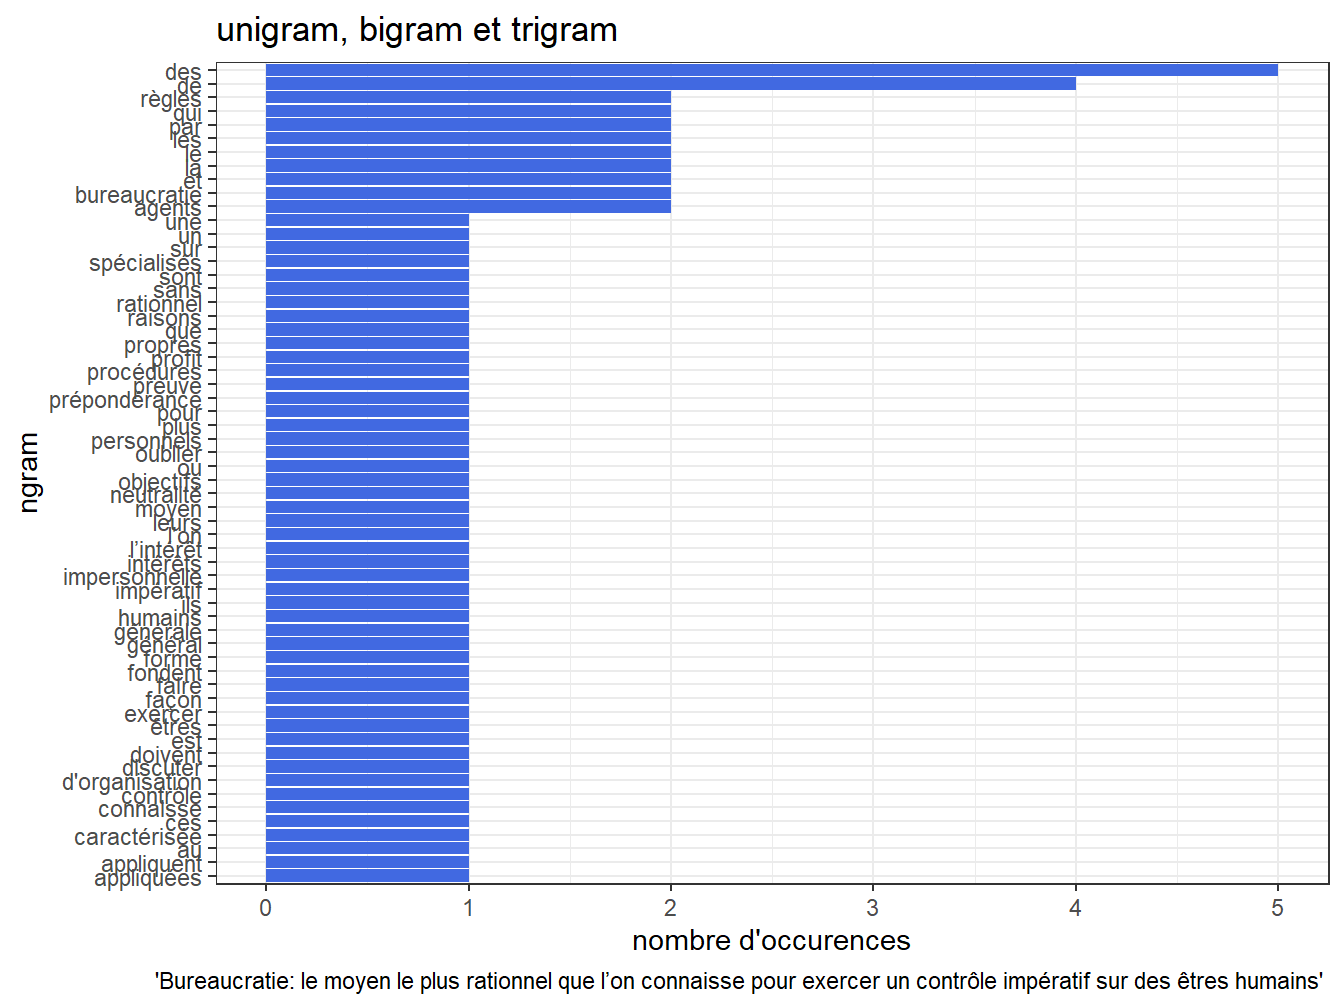
\includegraphics[width=0.8\linewidth]{bookdown-demo_files/figure-latex/503-1} 

}

\caption{Distribution du nombre de mots, sans les stopwords}\label{fig:503}
\end{figure}

On peut également constater que certains mots sont proches, par exemple les deux derniers sur le graphiques précédents qui sont des déclinaisons du verbe appliquer. Il peut alors être pertinent de regrouper ces différentes formes verbales (comme un mot au singulier et au pluriel, au féminin et au masculin, ou conjugué sous différentes formes), pour faciliter l'analyse. C'est ce qu'on fait avec les opérations de \emph{stemming} ou de lemmatisation, présentées au chapitre \ref{annot}.

\hypertarget{les-phrases}{%
\subsection{Les phrases}\label{les-phrases}}

On reproduit les mêmes opérations, mais cette fois sur les phrases de l'exemple précédent.

\begin{Shaded}
\begin{Highlighting}[]
\KeywordTok{tokenize_sentences}\NormalTok{(MaxWeber)}\OperatorTok\KeywordTok{as.data.frame}\NormalTok{()}\OperatorTok\KeywordTok{rename}\NormalTok{(}\DataTypeTok{tokens=}\DecValTok{1}\NormalTok{)}\OperatorTok\KeywordTok{flextable}\NormalTok{(}\DataTypeTok{cwidth =} \DecValTok{5}\NormalTok{)}
\end{Highlighting}
\end{Shaded}

\providecommand{\docline}[3]{\noalign{\global\setlength{\arrayrulewidth}{#1}}\arrayrulecolor[HTML]{#2}\cline{#3}}

\setlength{\tabcolsep}{2pt}

\renewcommand*{\arraystretch}{1.5}

\begin{longtable}[c]{|p{5.00in}}



\hhline{>{\arrayrulecolor[HTML]{666666}\global\arrayrulewidth=2pt}-}

\multicolumn{1}{!{\color[HTML]{000000}\vrule width 0pt}>{\raggedright}p{\dimexpr 5in+0\tabcolsep+0\arrayrulewidth}!{\color[HTML]{000000}\vrule width 0pt}}{\fontsize{11}{11}\selectfont{\textcolor[HTML]{000000}{\global\setmainfont{Arial}tokens}}} \\

\noalign{\global\setlength{\arrayrulewidth}{2pt}}\arrayrulecolor[HTML]{666666}\cline{1-1}

\endfirsthead

\hhline{>{\arrayrulecolor[HTML]{666666}\global\arrayrulewidth=2pt}-}

\multicolumn{1}{!{\color[HTML]{000000}\vrule width 0pt}>{\raggedright}p{\dimexpr 5in+0\tabcolsep+0\arrayrulewidth}!{\color[HTML]{000000}\vrule width 0pt}}{\fontsize{11}{11}\selectfont{\textcolor[HTML]{000000}{\global\setmainfont{Arial}tokens}}} \\

\noalign{\global\setlength{\arrayrulewidth}{2pt}}\arrayrulecolor[HTML]{666666}\cline{1-1}\endhead



\multicolumn{1}{!{\color[HTML]{000000}\vrule width 0pt}>{\raggedright}p{\dimexpr 5in+0\tabcolsep+0\arrayrulewidth}!{\color[HTML]{000000}\vrule width 0pt}}{\fontsize{11}{11}\selectfont{\textcolor[HTML]{000000}{\global\setmainfont{Arial}Bureaucratie:\ le\ moyen\ le\ plus\ rationnel\ que\ l’on\ connaisse\ pour\ exercer\ un\ contrôle\ impératif\ sur\ des\ êtres\ humains.}}} \\





\multicolumn{1}{!{\color[HTML]{000000}\vrule width 0pt}>{\raggedright}p{\dimexpr 5in+0\tabcolsep+0\arrayrulewidth}!{\color[HTML]{000000}\vrule width 0pt}}{\fontsize{11}{11}\selectfont{\textcolor[HTML]{000000}{\global\setmainfont{Arial}La\ bureaucratie\ est\ une\ forme\ d'organisation\ générale\ caractérisée\ par\ la\ prépondérance\ des\ règles\ et\ de\ procédures\ qui\ sont\ appliquées\ de\ façon\ impersonnelle\ par\ des\ agents\ spécialisés.}}} \\





\multicolumn{1}{!{\color[HTML]{000000}\vrule width 0pt}>{\raggedright}p{\dimexpr 5in+0\tabcolsep+0\arrayrulewidth}!{\color[HTML]{000000}\vrule width 0pt}}{\fontsize{11}{11}\selectfont{\textcolor[HTML]{000000}{\global\setmainfont{Arial}Ces\ agents\ appliquent\ les\ règles\ sans\ discuter\ des\ objectifs\ ou\ des\ raisons\ qui\ les\ fondent.}}} \\





\multicolumn{1}{!{\color[HTML]{000000}\vrule width 0pt}>{\raggedright}p{\dimexpr 5in+0\tabcolsep+0\arrayrulewidth}!{\color[HTML]{000000}\vrule width 0pt}}{\fontsize{11}{11}\selectfont{\textcolor[HTML]{000000}{\global\setmainfont{Arial}Ils\ doivent\ faire\ preuve\ de\ neutralité\ et\ oublier\ leurs\ propres\ intérêts\ personnels\ au\ profit\ de\ l’intérêt\ général.}}} \\

\noalign{\global\setlength{\arrayrulewidth}{2pt}}\arrayrulecolor[HTML]{666666}\cline{1-1}

\end{longtable}

\hypertarget{n-grammes}{%
\section{N-grammes}\label{n-grammes}}

Les n-grammes sont des séquences de n \emph{tokens}, généralement consécutifs. Voici tout de suite un exemple sur les lettres\footnote{Le principe de `textcat' est fondée sur ces n-grammes de lettre. Chaque langue se caractérise par une distribution particulière des n-grammes. Pour décider de l'appartenance d'un texte à une langue, si on dispose des profils de distribution, on compare la distribution des n-grammes du texte à ces références. On peut ainsi calculer une distance et attribuer le texte à la langue dont il est le plus proche.}, allant de bigramme au trigramme :

\begin{Shaded}
\begin{Highlighting}[]
\NormalTok{toc_maxweber<-}\KeywordTok{tokenize_character_shingles}\NormalTok{(MaxWeber,}\DataTypeTok{n=}\DecValTok{3}\NormalTok{, }\DataTypeTok{n_min=}\DecValTok{2}\NormalTok{) }\OperatorTok
\StringTok{        }\KeywordTok{as.data.frame}\NormalTok{()}\OperatorTok\KeywordTok{rename}\NormalTok{(}\DataTypeTok{tokens=}\DecValTok{1}\NormalTok{)}
\KeywordTok{flextable}\NormalTok{(}\KeywordTok{head}\NormalTok{(toc_maxweber, }\DataTypeTok{n=}\DecValTok{20}\NormalTok{))}
\end{Highlighting}
\end{Shaded}

\providecommand{\docline}[3]{\noalign{\global\setlength{\arrayrulewidth}{#1}}\arrayrulecolor[HTML]{#2}\cline{#3}}

\setlength{\tabcolsep}{2pt}

\renewcommand*{\arraystretch}{1.5}

\begin{longtable}[c]{|p{0.75in}}



\hhline{>{\arrayrulecolor[HTML]{666666}\global\arrayrulewidth=2pt}-}

\multicolumn{1}{!{\color[HTML]{000000}\vrule width 0pt}>{\raggedright}p{\dimexpr 0.75in+0\tabcolsep+0\arrayrulewidth}!{\color[HTML]{000000}\vrule width 0pt}}{\fontsize{11}{11}\selectfont{\textcolor[HTML]{000000}{\global\setmainfont{Arial}tokens}}} \\

\noalign{\global\setlength{\arrayrulewidth}{2pt}}\arrayrulecolor[HTML]{666666}\cline{1-1}

\endfirsthead

\hhline{>{\arrayrulecolor[HTML]{666666}\global\arrayrulewidth=2pt}-}

\multicolumn{1}{!{\color[HTML]{000000}\vrule width 0pt}>{\raggedright}p{\dimexpr 0.75in+0\tabcolsep+0\arrayrulewidth}!{\color[HTML]{000000}\vrule width 0pt}}{\fontsize{11}{11}\selectfont{\textcolor[HTML]{000000}{\global\setmainfont{Arial}tokens}}} \\

\noalign{\global\setlength{\arrayrulewidth}{2pt}}\arrayrulecolor[HTML]{666666}\cline{1-1}\endhead



\multicolumn{1}{!{\color[HTML]{000000}\vrule width 0pt}>{\raggedright}p{\dimexpr 0.75in+0\tabcolsep+0\arrayrulewidth}!{\color[HTML]{000000}\vrule width 0pt}}{\fontsize{11}{11}\selectfont{\textcolor[HTML]{000000}{\global\setmainfont{Arial}bu}}} \\





\multicolumn{1}{!{\color[HTML]{000000}\vrule width 0pt}>{\raggedright}p{\dimexpr 0.75in+0\tabcolsep+0\arrayrulewidth}!{\color[HTML]{000000}\vrule width 0pt}}{\fontsize{11}{11}\selectfont{\textcolor[HTML]{000000}{\global\setmainfont{Arial}bur}}} \\





\multicolumn{1}{!{\color[HTML]{000000}\vrule width 0pt}>{\raggedright}p{\dimexpr 0.75in+0\tabcolsep+0\arrayrulewidth}!{\color[HTML]{000000}\vrule width 0pt}}{\fontsize{11}{11}\selectfont{\textcolor[HTML]{000000}{\global\setmainfont{Arial}ur}}} \\





\multicolumn{1}{!{\color[HTML]{000000}\vrule width 0pt}>{\raggedright}p{\dimexpr 0.75in+0\tabcolsep+0\arrayrulewidth}!{\color[HTML]{000000}\vrule width 0pt}}{\fontsize{11}{11}\selectfont{\textcolor[HTML]{000000}{\global\setmainfont{Arial}ure}}} \\





\multicolumn{1}{!{\color[HTML]{000000}\vrule width 0pt}>{\raggedright}p{\dimexpr 0.75in+0\tabcolsep+0\arrayrulewidth}!{\color[HTML]{000000}\vrule width 0pt}}{\fontsize{11}{11}\selectfont{\textcolor[HTML]{000000}{\global\setmainfont{Arial}re}}} \\





\multicolumn{1}{!{\color[HTML]{000000}\vrule width 0pt}>{\raggedright}p{\dimexpr 0.75in+0\tabcolsep+0\arrayrulewidth}!{\color[HTML]{000000}\vrule width 0pt}}{\fontsize{11}{11}\selectfont{\textcolor[HTML]{000000}{\global\setmainfont{Arial}rea}}} \\





\multicolumn{1}{!{\color[HTML]{000000}\vrule width 0pt}>{\raggedright}p{\dimexpr 0.75in+0\tabcolsep+0\arrayrulewidth}!{\color[HTML]{000000}\vrule width 0pt}}{\fontsize{11}{11}\selectfont{\textcolor[HTML]{000000}{\global\setmainfont{Arial}ea}}} \\





\multicolumn{1}{!{\color[HTML]{000000}\vrule width 0pt}>{\raggedright}p{\dimexpr 0.75in+0\tabcolsep+0\arrayrulewidth}!{\color[HTML]{000000}\vrule width 0pt}}{\fontsize{11}{11}\selectfont{\textcolor[HTML]{000000}{\global\setmainfont{Arial}eau}}} \\





\multicolumn{1}{!{\color[HTML]{000000}\vrule width 0pt}>{\raggedright}p{\dimexpr 0.75in+0\tabcolsep+0\arrayrulewidth}!{\color[HTML]{000000}\vrule width 0pt}}{\fontsize{11}{11}\selectfont{\textcolor[HTML]{000000}{\global\setmainfont{Arial}au}}} \\





\multicolumn{1}{!{\color[HTML]{000000}\vrule width 0pt}>{\raggedright}p{\dimexpr 0.75in+0\tabcolsep+0\arrayrulewidth}!{\color[HTML]{000000}\vrule width 0pt}}{\fontsize{11}{11}\selectfont{\textcolor[HTML]{000000}{\global\setmainfont{Arial}auc}}} \\





\multicolumn{1}{!{\color[HTML]{000000}\vrule width 0pt}>{\raggedright}p{\dimexpr 0.75in+0\tabcolsep+0\arrayrulewidth}!{\color[HTML]{000000}\vrule width 0pt}}{\fontsize{11}{11}\selectfont{\textcolor[HTML]{000000}{\global\setmainfont{Arial}uc}}} \\





\multicolumn{1}{!{\color[HTML]{000000}\vrule width 0pt}>{\raggedright}p{\dimexpr 0.75in+0\tabcolsep+0\arrayrulewidth}!{\color[HTML]{000000}\vrule width 0pt}}{\fontsize{11}{11}\selectfont{\textcolor[HTML]{000000}{\global\setmainfont{Arial}ucr}}} \\





\multicolumn{1}{!{\color[HTML]{000000}\vrule width 0pt}>{\raggedright}p{\dimexpr 0.75in+0\tabcolsep+0\arrayrulewidth}!{\color[HTML]{000000}\vrule width 0pt}}{\fontsize{11}{11}\selectfont{\textcolor[HTML]{000000}{\global\setmainfont{Arial}cr}}} \\





\multicolumn{1}{!{\color[HTML]{000000}\vrule width 0pt}>{\raggedright}p{\dimexpr 0.75in+0\tabcolsep+0\arrayrulewidth}!{\color[HTML]{000000}\vrule width 0pt}}{\fontsize{11}{11}\selectfont{\textcolor[HTML]{000000}{\global\setmainfont{Arial}cra}}} \\





\multicolumn{1}{!{\color[HTML]{000000}\vrule width 0pt}>{\raggedright}p{\dimexpr 0.75in+0\tabcolsep+0\arrayrulewidth}!{\color[HTML]{000000}\vrule width 0pt}}{\fontsize{11}{11}\selectfont{\textcolor[HTML]{000000}{\global\setmainfont{Arial}ra}}} \\





\multicolumn{1}{!{\color[HTML]{000000}\vrule width 0pt}>{\raggedright}p{\dimexpr 0.75in+0\tabcolsep+0\arrayrulewidth}!{\color[HTML]{000000}\vrule width 0pt}}{\fontsize{11}{11}\selectfont{\textcolor[HTML]{000000}{\global\setmainfont{Arial}rat}}} \\





\multicolumn{1}{!{\color[HTML]{000000}\vrule width 0pt}>{\raggedright}p{\dimexpr 0.75in+0\tabcolsep+0\arrayrulewidth}!{\color[HTML]{000000}\vrule width 0pt}}{\fontsize{11}{11}\selectfont{\textcolor[HTML]{000000}{\global\setmainfont{Arial}at}}} \\





\multicolumn{1}{!{\color[HTML]{000000}\vrule width 0pt}>{\raggedright}p{\dimexpr 0.75in+0\tabcolsep+0\arrayrulewidth}!{\color[HTML]{000000}\vrule width 0pt}}{\fontsize{11}{11}\selectfont{\textcolor[HTML]{000000}{\global\setmainfont{Arial}ati}}} \\





\multicolumn{1}{!{\color[HTML]{000000}\vrule width 0pt}>{\raggedright}p{\dimexpr 0.75in+0\tabcolsep+0\arrayrulewidth}!{\color[HTML]{000000}\vrule width 0pt}}{\fontsize{11}{11}\selectfont{\textcolor[HTML]{000000}{\global\setmainfont{Arial}ti}}} \\





\multicolumn{1}{!{\color[HTML]{000000}\vrule width 0pt}>{\raggedright}p{\dimexpr 0.75in+0\tabcolsep+0\arrayrulewidth}!{\color[HTML]{000000}\vrule width 0pt}}{\fontsize{11}{11}\selectfont{\textcolor[HTML]{000000}{\global\setmainfont{Arial}tie}}} \\

\noalign{\global\setlength{\arrayrulewidth}{2pt}}\arrayrulecolor[HTML]{666666}\cline{1-1}

\end{longtable}

\begin{Shaded}
\begin{Highlighting}[]
\NormalTok{foo<-toc_maxweber }\OperatorTok\KeywordTok{mutate}\NormalTok{(}\DataTypeTok{n=}\DecValTok{1}\NormalTok{) }\OperatorTok\StringTok{ }
\StringTok{        }\KeywordTok{group_by}\NormalTok{(tokens)}\OperatorTok\StringTok{ }
\StringTok{        }\KeywordTok{summarise}\NormalTok{(}\DataTypeTok{n=}\KeywordTok{sum}\NormalTok{(n))}\OperatorTok\KeywordTok{filter}\NormalTok{(n}\OperatorTok{>}\DecValTok{3}\NormalTok{)}

\KeywordTok{ggplot}\NormalTok{(foo, }\KeywordTok{aes}\NormalTok{(}\DataTypeTok{x=}\KeywordTok{reorder}\NormalTok{(tokens,n), }\DataTypeTok{y=}\NormalTok{n))}\OperatorTok{+}
\StringTok{               }\KeywordTok{geom_bar}\NormalTok{(}\DataTypeTok{stat=}\StringTok{"identity"}\NormalTok{, }\DataTypeTok{fill=}\StringTok{"royalblue"}\NormalTok{)}\OperatorTok{+}\KeywordTok{annotate}\NormalTok{(}\StringTok{"text"}\NormalTok{, }\DataTypeTok{x=}\DecValTok{5}\NormalTok{,}\DataTypeTok{y=}\DecValTok{11}\NormalTok{, }\DataTypeTok{label=}\KeywordTok{paste}\NormalTok{(}\StringTok{"nombre de tokens ="}\NormalTok{, }\KeywordTok{nrow}\NormalTok{(toc_maxweber)))}\OperatorTok{+}
\StringTok{               }\KeywordTok{coord_flip}\NormalTok{()}\OperatorTok{+}\KeywordTok{labs}\NormalTok{(}\DataTypeTok{title =} \StringTok{"Bigrammes et trigrammes des lettres"}\NormalTok{, }\DataTypeTok{x=}\StringTok{"n-gramme"}\NormalTok{, }\DataTypeTok{y=}\StringTok{"nombre d'occurences"}\NormalTok{)}
\end{Highlighting}
\end{Shaded}

\begin{figure}

{\centering 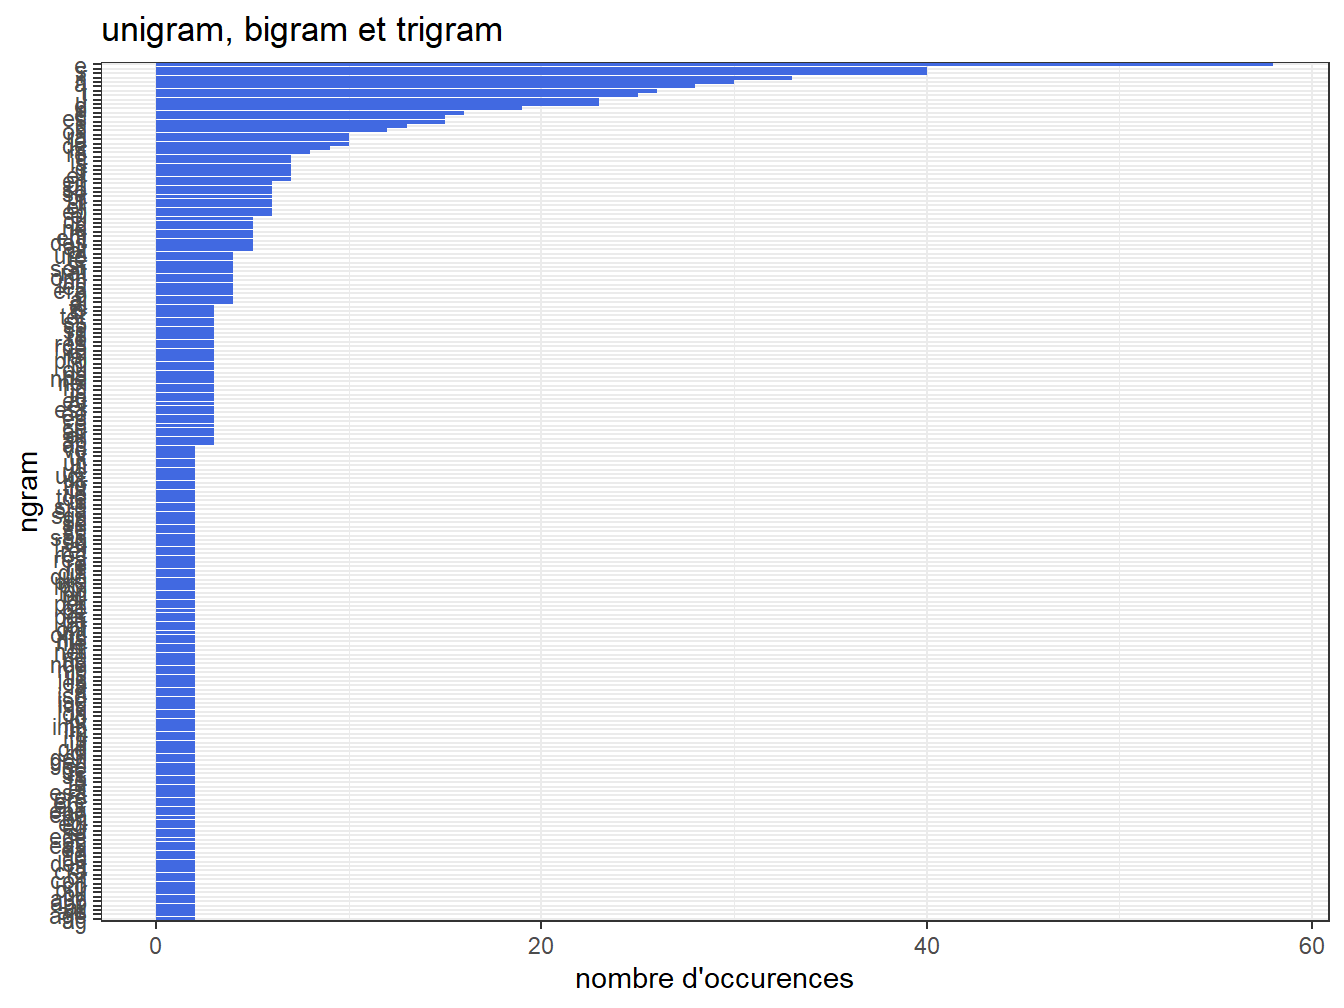
\includegraphics[width=0.8\linewidth]{bookdown-demo_files/figure-latex/505-1} 

}

\caption{Bigrammes et trigrammes de lettres}\label{fig:505}
\end{figure}

On peut faire la même chose sur les mots, en éliminant les \emph{stopwords} :

\begin{Shaded}
\begin{Highlighting}[]
\NormalTok{toc_maxweber<-}\KeywordTok{tokenize_ngrams}\NormalTok{(MaxWeber,}\DataTypeTok{n=}\DecValTok{3}\NormalTok{, }\DataTypeTok{n_min=}\DecValTok{2}\NormalTok{, }\DataTypeTok{stopwords =} \KeywordTok{stopwords}\NormalTok{(}\StringTok{'fr'}\NormalTok{)) }\OperatorTok
\StringTok{        }\KeywordTok{as.data.frame}\NormalTok{()}\OperatorTok\KeywordTok{rename}\NormalTok{(}\DataTypeTok{tokens=}\DecValTok{1}\NormalTok{)}
\KeywordTok{qflextable}\NormalTok{(}\KeywordTok{head}\NormalTok{(toc_maxweber, }\DataTypeTok{n=}\DecValTok{19}\NormalTok{))}
\end{Highlighting}
\end{Shaded}

\providecommand{\docline}[3]{\noalign{\global\setlength{\arrayrulewidth}{#1}}\arrayrulecolor[HTML]{#2}\cline{#3}}

\setlength{\tabcolsep}{2pt}

\renewcommand*{\arraystretch}{1.5}

\begin{longtable}[c]{|p{2.11in}}



\hhline{>{\arrayrulecolor[HTML]{666666}\global\arrayrulewidth=2pt}-}

\multicolumn{1}{!{\color[HTML]{000000}\vrule width 0pt}>{\raggedright}p{\dimexpr 2.11in+0\tabcolsep+0\arrayrulewidth}!{\color[HTML]{000000}\vrule width 0pt}}{\fontsize{11}{11}\selectfont{\textcolor[HTML]{000000}{\global\setmainfont{Arial}tokens}}} \\

\noalign{\global\setlength{\arrayrulewidth}{2pt}}\arrayrulecolor[HTML]{666666}\cline{1-1}

\endfirsthead

\hhline{>{\arrayrulecolor[HTML]{666666}\global\arrayrulewidth=2pt}-}

\multicolumn{1}{!{\color[HTML]{000000}\vrule width 0pt}>{\raggedright}p{\dimexpr 2.11in+0\tabcolsep+0\arrayrulewidth}!{\color[HTML]{000000}\vrule width 0pt}}{\fontsize{11}{11}\selectfont{\textcolor[HTML]{000000}{\global\setmainfont{Arial}tokens}}} \\

\noalign{\global\setlength{\arrayrulewidth}{2pt}}\arrayrulecolor[HTML]{666666}\cline{1-1}\endhead



\multicolumn{1}{!{\color[HTML]{000000}\vrule width 0pt}>{\raggedright}p{\dimexpr 2.11in+0\tabcolsep+0\arrayrulewidth}!{\color[HTML]{000000}\vrule width 0pt}}{\fontsize{11}{11}\selectfont{\textcolor[HTML]{000000}{\global\setmainfont{Arial}bureaucratie\ moyen}}} \\





\multicolumn{1}{!{\color[HTML]{000000}\vrule width 0pt}>{\raggedright}p{\dimexpr 2.11in+0\tabcolsep+0\arrayrulewidth}!{\color[HTML]{000000}\vrule width 0pt}}{\fontsize{11}{11}\selectfont{\textcolor[HTML]{000000}{\global\setmainfont{Arial}bureaucratie\ moyen\ plus}}} \\





\multicolumn{1}{!{\color[HTML]{000000}\vrule width 0pt}>{\raggedright}p{\dimexpr 2.11in+0\tabcolsep+0\arrayrulewidth}!{\color[HTML]{000000}\vrule width 0pt}}{\fontsize{11}{11}\selectfont{\textcolor[HTML]{000000}{\global\setmainfont{Arial}moyen\ plus}}} \\





\multicolumn{1}{!{\color[HTML]{000000}\vrule width 0pt}>{\raggedright}p{\dimexpr 2.11in+0\tabcolsep+0\arrayrulewidth}!{\color[HTML]{000000}\vrule width 0pt}}{\fontsize{11}{11}\selectfont{\textcolor[HTML]{000000}{\global\setmainfont{Arial}moyen\ plus\ rationnel}}} \\





\multicolumn{1}{!{\color[HTML]{000000}\vrule width 0pt}>{\raggedright}p{\dimexpr 2.11in+0\tabcolsep+0\arrayrulewidth}!{\color[HTML]{000000}\vrule width 0pt}}{\fontsize{11}{11}\selectfont{\textcolor[HTML]{000000}{\global\setmainfont{Arial}plus\ rationnel}}} \\





\multicolumn{1}{!{\color[HTML]{000000}\vrule width 0pt}>{\raggedright}p{\dimexpr 2.11in+0\tabcolsep+0\arrayrulewidth}!{\color[HTML]{000000}\vrule width 0pt}}{\fontsize{11}{11}\selectfont{\textcolor[HTML]{000000}{\global\setmainfont{Arial}plus\ rationnel\ l’on}}} \\





\multicolumn{1}{!{\color[HTML]{000000}\vrule width 0pt}>{\raggedright}p{\dimexpr 2.11in+0\tabcolsep+0\arrayrulewidth}!{\color[HTML]{000000}\vrule width 0pt}}{\fontsize{11}{11}\selectfont{\textcolor[HTML]{000000}{\global\setmainfont{Arial}rationnel\ l’on}}} \\





\multicolumn{1}{!{\color[HTML]{000000}\vrule width 0pt}>{\raggedright}p{\dimexpr 2.11in+0\tabcolsep+0\arrayrulewidth}!{\color[HTML]{000000}\vrule width 0pt}}{\fontsize{11}{11}\selectfont{\textcolor[HTML]{000000}{\global\setmainfont{Arial}rationnel\ l’on\ connaisse}}} \\





\multicolumn{1}{!{\color[HTML]{000000}\vrule width 0pt}>{\raggedright}p{\dimexpr 2.11in+0\tabcolsep+0\arrayrulewidth}!{\color[HTML]{000000}\vrule width 0pt}}{\fontsize{11}{11}\selectfont{\textcolor[HTML]{000000}{\global\setmainfont{Arial}l’on\ connaisse}}} \\





\multicolumn{1}{!{\color[HTML]{000000}\vrule width 0pt}>{\raggedright}p{\dimexpr 2.11in+0\tabcolsep+0\arrayrulewidth}!{\color[HTML]{000000}\vrule width 0pt}}{\fontsize{11}{11}\selectfont{\textcolor[HTML]{000000}{\global\setmainfont{Arial}l’on\ connaisse\ exercer}}} \\





\multicolumn{1}{!{\color[HTML]{000000}\vrule width 0pt}>{\raggedright}p{\dimexpr 2.11in+0\tabcolsep+0\arrayrulewidth}!{\color[HTML]{000000}\vrule width 0pt}}{\fontsize{11}{11}\selectfont{\textcolor[HTML]{000000}{\global\setmainfont{Arial}connaisse\ exercer}}} \\





\multicolumn{1}{!{\color[HTML]{000000}\vrule width 0pt}>{\raggedright}p{\dimexpr 2.11in+0\tabcolsep+0\arrayrulewidth}!{\color[HTML]{000000}\vrule width 0pt}}{\fontsize{11}{11}\selectfont{\textcolor[HTML]{000000}{\global\setmainfont{Arial}connaisse\ exercer\ contrôle}}} \\





\multicolumn{1}{!{\color[HTML]{000000}\vrule width 0pt}>{\raggedright}p{\dimexpr 2.11in+0\tabcolsep+0\arrayrulewidth}!{\color[HTML]{000000}\vrule width 0pt}}{\fontsize{11}{11}\selectfont{\textcolor[HTML]{000000}{\global\setmainfont{Arial}exercer\ contrôle}}} \\





\multicolumn{1}{!{\color[HTML]{000000}\vrule width 0pt}>{\raggedright}p{\dimexpr 2.11in+0\tabcolsep+0\arrayrulewidth}!{\color[HTML]{000000}\vrule width 0pt}}{\fontsize{11}{11}\selectfont{\textcolor[HTML]{000000}{\global\setmainfont{Arial}exercer\ contrôle\ impératif}}} \\





\multicolumn{1}{!{\color[HTML]{000000}\vrule width 0pt}>{\raggedright}p{\dimexpr 2.11in+0\tabcolsep+0\arrayrulewidth}!{\color[HTML]{000000}\vrule width 0pt}}{\fontsize{11}{11}\selectfont{\textcolor[HTML]{000000}{\global\setmainfont{Arial}contrôle\ impératif}}} \\





\multicolumn{1}{!{\color[HTML]{000000}\vrule width 0pt}>{\raggedright}p{\dimexpr 2.11in+0\tabcolsep+0\arrayrulewidth}!{\color[HTML]{000000}\vrule width 0pt}}{\fontsize{11}{11}\selectfont{\textcolor[HTML]{000000}{\global\setmainfont{Arial}contrôle\ impératif\ êtres}}} \\





\multicolumn{1}{!{\color[HTML]{000000}\vrule width 0pt}>{\raggedright}p{\dimexpr 2.11in+0\tabcolsep+0\arrayrulewidth}!{\color[HTML]{000000}\vrule width 0pt}}{\fontsize{11}{11}\selectfont{\textcolor[HTML]{000000}{\global\setmainfont{Arial}impératif\ êtres}}} \\





\multicolumn{1}{!{\color[HTML]{000000}\vrule width 0pt}>{\raggedright}p{\dimexpr 2.11in+0\tabcolsep+0\arrayrulewidth}!{\color[HTML]{000000}\vrule width 0pt}}{\fontsize{11}{11}\selectfont{\textcolor[HTML]{000000}{\global\setmainfont{Arial}impératif\ êtres\ humains}}} \\





\multicolumn{1}{!{\color[HTML]{000000}\vrule width 0pt}>{\raggedright}p{\dimexpr 2.11in+0\tabcolsep+0\arrayrulewidth}!{\color[HTML]{000000}\vrule width 0pt}}{\fontsize{11}{11}\selectfont{\textcolor[HTML]{000000}{\global\setmainfont{Arial}êtres\ humains}}} \\

\noalign{\global\setlength{\arrayrulewidth}{2pt}}\arrayrulecolor[HTML]{666666}\cline{1-1}

\end{longtable}

On peut également s'intéresser aux n-grammes non directement consécutifs mais séparés par k \emph{tokens} :

\begin{Shaded}
\begin{Highlighting}[]
\NormalTok{toc_maxweber<-}\KeywordTok{tokenize_skip_ngrams}\NormalTok{(MaxWeber,}\DataTypeTok{n=}\DecValTok{3}\NormalTok{, }\DataTypeTok{n_min=}\DecValTok{2}\NormalTok{, }\DataTypeTok{k=}\DecValTok{2}\NormalTok{, }\DataTypeTok{stopwords =} \KeywordTok{stopwords}\NormalTok{(}\StringTok{'fr'}\NormalTok{)) }\OperatorTok
\StringTok{        }\KeywordTok{as.data.frame}\NormalTok{()}\OperatorTok\KeywordTok{rename}\NormalTok{(}\DataTypeTok{tokens=}\DecValTok{1}\NormalTok{)}
\KeywordTok{qflextable}\NormalTok{(}\KeywordTok{head}\NormalTok{(toc_maxweber, }\DataTypeTok{n=}\DecValTok{19}\NormalTok{))}
\end{Highlighting}
\end{Shaded}

\providecommand{\docline}[3]{\noalign{\global\setlength{\arrayrulewidth}{#1}}\arrayrulecolor[HTML]{#2}\cline{#3}}

\setlength{\tabcolsep}{2pt}

\renewcommand*{\arraystretch}{1.5}

\begin{longtable}[c]{|p{2.49in}}



\hhline{>{\arrayrulecolor[HTML]{666666}\global\arrayrulewidth=2pt}-}

\multicolumn{1}{!{\color[HTML]{000000}\vrule width 0pt}>{\raggedright}p{\dimexpr 2.49in+0\tabcolsep+0\arrayrulewidth}!{\color[HTML]{000000}\vrule width 0pt}}{\fontsize{11}{11}\selectfont{\textcolor[HTML]{000000}{\global\setmainfont{Arial}tokens}}} \\

\noalign{\global\setlength{\arrayrulewidth}{2pt}}\arrayrulecolor[HTML]{666666}\cline{1-1}

\endfirsthead

\hhline{>{\arrayrulecolor[HTML]{666666}\global\arrayrulewidth=2pt}-}

\multicolumn{1}{!{\color[HTML]{000000}\vrule width 0pt}>{\raggedright}p{\dimexpr 2.49in+0\tabcolsep+0\arrayrulewidth}!{\color[HTML]{000000}\vrule width 0pt}}{\fontsize{11}{11}\selectfont{\textcolor[HTML]{000000}{\global\setmainfont{Arial}tokens}}} \\

\noalign{\global\setlength{\arrayrulewidth}{2pt}}\arrayrulecolor[HTML]{666666}\cline{1-1}\endhead



\multicolumn{1}{!{\color[HTML]{000000}\vrule width 0pt}>{\raggedright}p{\dimexpr 2.49in+0\tabcolsep+0\arrayrulewidth}!{\color[HTML]{000000}\vrule width 0pt}}{\fontsize{11}{11}\selectfont{\textcolor[HTML]{000000}{\global\setmainfont{Arial}bureaucratie\ moyen}}} \\





\multicolumn{1}{!{\color[HTML]{000000}\vrule width 0pt}>{\raggedright}p{\dimexpr 2.49in+0\tabcolsep+0\arrayrulewidth}!{\color[HTML]{000000}\vrule width 0pt}}{\fontsize{11}{11}\selectfont{\textcolor[HTML]{000000}{\global\setmainfont{Arial}bureaucratie\ plus}}} \\





\multicolumn{1}{!{\color[HTML]{000000}\vrule width 0pt}>{\raggedright}p{\dimexpr 2.49in+0\tabcolsep+0\arrayrulewidth}!{\color[HTML]{000000}\vrule width 0pt}}{\fontsize{11}{11}\selectfont{\textcolor[HTML]{000000}{\global\setmainfont{Arial}bureaucratie\ rationnel}}} \\





\multicolumn{1}{!{\color[HTML]{000000}\vrule width 0pt}>{\raggedright}p{\dimexpr 2.49in+0\tabcolsep+0\arrayrulewidth}!{\color[HTML]{000000}\vrule width 0pt}}{\fontsize{11}{11}\selectfont{\textcolor[HTML]{000000}{\global\setmainfont{Arial}bureaucratie\ moyen\ plus}}} \\





\multicolumn{1}{!{\color[HTML]{000000}\vrule width 0pt}>{\raggedright}p{\dimexpr 2.49in+0\tabcolsep+0\arrayrulewidth}!{\color[HTML]{000000}\vrule width 0pt}}{\fontsize{11}{11}\selectfont{\textcolor[HTML]{000000}{\global\setmainfont{Arial}bureaucratie\ moyen\ rationnel}}} \\





\multicolumn{1}{!{\color[HTML]{000000}\vrule width 0pt}>{\raggedright}p{\dimexpr 2.49in+0\tabcolsep+0\arrayrulewidth}!{\color[HTML]{000000}\vrule width 0pt}}{\fontsize{11}{11}\selectfont{\textcolor[HTML]{000000}{\global\setmainfont{Arial}bureaucratie\ moyen\ l’on}}} \\





\multicolumn{1}{!{\color[HTML]{000000}\vrule width 0pt}>{\raggedright}p{\dimexpr 2.49in+0\tabcolsep+0\arrayrulewidth}!{\color[HTML]{000000}\vrule width 0pt}}{\fontsize{11}{11}\selectfont{\textcolor[HTML]{000000}{\global\setmainfont{Arial}bureaucratie\ plus\ rationnel}}} \\





\multicolumn{1}{!{\color[HTML]{000000}\vrule width 0pt}>{\raggedright}p{\dimexpr 2.49in+0\tabcolsep+0\arrayrulewidth}!{\color[HTML]{000000}\vrule width 0pt}}{\fontsize{11}{11}\selectfont{\textcolor[HTML]{000000}{\global\setmainfont{Arial}bureaucratie\ plus\ l’on}}} \\





\multicolumn{1}{!{\color[HTML]{000000}\vrule width 0pt}>{\raggedright}p{\dimexpr 2.49in+0\tabcolsep+0\arrayrulewidth}!{\color[HTML]{000000}\vrule width 0pt}}{\fontsize{11}{11}\selectfont{\textcolor[HTML]{000000}{\global\setmainfont{Arial}bureaucratie\ plus\ connaisse}}} \\





\multicolumn{1}{!{\color[HTML]{000000}\vrule width 0pt}>{\raggedright}p{\dimexpr 2.49in+0\tabcolsep+0\arrayrulewidth}!{\color[HTML]{000000}\vrule width 0pt}}{\fontsize{11}{11}\selectfont{\textcolor[HTML]{000000}{\global\setmainfont{Arial}bureaucratie\ rationnel\ l’on}}} \\





\multicolumn{1}{!{\color[HTML]{000000}\vrule width 0pt}>{\raggedright}p{\dimexpr 2.49in+0\tabcolsep+0\arrayrulewidth}!{\color[HTML]{000000}\vrule width 0pt}}{\fontsize{11}{11}\selectfont{\textcolor[HTML]{000000}{\global\setmainfont{Arial}bureaucratie\ rationnel\ connaisse}}} \\





\multicolumn{1}{!{\color[HTML]{000000}\vrule width 0pt}>{\raggedright}p{\dimexpr 2.49in+0\tabcolsep+0\arrayrulewidth}!{\color[HTML]{000000}\vrule width 0pt}}{\fontsize{11}{11}\selectfont{\textcolor[HTML]{000000}{\global\setmainfont{Arial}bureaucratie\ rationnel\ exercer}}} \\





\multicolumn{1}{!{\color[HTML]{000000}\vrule width 0pt}>{\raggedright}p{\dimexpr 2.49in+0\tabcolsep+0\arrayrulewidth}!{\color[HTML]{000000}\vrule width 0pt}}{\fontsize{11}{11}\selectfont{\textcolor[HTML]{000000}{\global\setmainfont{Arial}moyen\ plus}}} \\





\multicolumn{1}{!{\color[HTML]{000000}\vrule width 0pt}>{\raggedright}p{\dimexpr 2.49in+0\tabcolsep+0\arrayrulewidth}!{\color[HTML]{000000}\vrule width 0pt}}{\fontsize{11}{11}\selectfont{\textcolor[HTML]{000000}{\global\setmainfont{Arial}moyen\ rationnel}}} \\





\multicolumn{1}{!{\color[HTML]{000000}\vrule width 0pt}>{\raggedright}p{\dimexpr 2.49in+0\tabcolsep+0\arrayrulewidth}!{\color[HTML]{000000}\vrule width 0pt}}{\fontsize{11}{11}\selectfont{\textcolor[HTML]{000000}{\global\setmainfont{Arial}moyen\ l’on}}} \\





\multicolumn{1}{!{\color[HTML]{000000}\vrule width 0pt}>{\raggedright}p{\dimexpr 2.49in+0\tabcolsep+0\arrayrulewidth}!{\color[HTML]{000000}\vrule width 0pt}}{\fontsize{11}{11}\selectfont{\textcolor[HTML]{000000}{\global\setmainfont{Arial}moyen\ plus\ rationnel}}} \\





\multicolumn{1}{!{\color[HTML]{000000}\vrule width 0pt}>{\raggedright}p{\dimexpr 2.49in+0\tabcolsep+0\arrayrulewidth}!{\color[HTML]{000000}\vrule width 0pt}}{\fontsize{11}{11}\selectfont{\textcolor[HTML]{000000}{\global\setmainfont{Arial}moyen\ plus\ l’on}}} \\





\multicolumn{1}{!{\color[HTML]{000000}\vrule width 0pt}>{\raggedright}p{\dimexpr 2.49in+0\tabcolsep+0\arrayrulewidth}!{\color[HTML]{000000}\vrule width 0pt}}{\fontsize{11}{11}\selectfont{\textcolor[HTML]{000000}{\global\setmainfont{Arial}moyen\ plus\ connaisse}}} \\





\multicolumn{1}{!{\color[HTML]{000000}\vrule width 0pt}>{\raggedright}p{\dimexpr 2.49in+0\tabcolsep+0\arrayrulewidth}!{\color[HTML]{000000}\vrule width 0pt}}{\fontsize{11}{11}\selectfont{\textcolor[HTML]{000000}{\global\setmainfont{Arial}moyen\ rationnel\ l’on}}} \\

\noalign{\global\setlength{\arrayrulewidth}{2pt}}\arrayrulecolor[HTML]{666666}\cline{1-1}

\end{longtable}

Dans cet exemple, aucun n-gramme n'est répété, mais c'est rarement le cas avec des corpus plus importants. Dans ce cas, une forte répétition de n-grammes est un indice d'une unité sémantique composée de plusieurs \emph{tokens} que l'on peut alors regrouper en un seul et même \emph{token}. C'est ce que l'on verra dans la section suivante, avec l'utilisation de `quanteda'.

\hypertarget{propriuxe9tuxe9s-statistiques-des-n-grammes}{%
\subsection{Propriétés statistiques des n-grammes}\label{propriuxe9tuxe9s-statistiques-des-n-grammes}}

Sur la d'un base d'un corpus important on peut calculer les probabilité d'apparitions d'un n-gramme. C'est une ressource que fournit Google
avec son \href{https://books.google.com/ngrams/}{Books Ngram Viewer}.

\href{https://fr.wikipedia.org/wiki/N-gramme}{Processus de markov}

application à la correction

\hypertarget{choisir-des-n-grammes-pertinents}{%
\section{Choisir des n-grammes pertinents}\label{choisir-des-n-grammes-pertinents}}

Dans ce livre l'unité principales d'analyse restera le mot. Mais nous savons, au moins intuitivement que certaines combinaisons de mots représentent des expressions qui ont la valeur d'un mot, une valeur sémantique, par exemple, l'expression ``Assemblée Nationale''. Ces deux mots réunis constituent un syntagme, une unité de sens. La question qui se pose est alors de savoir comment les identifier dans le flot des n-grammes ?

La technique est simple : si deux mots se retrouvent dans un ordre donné plus fréquemment que ce que le produit de leurs probabilités d'apparition laisse espérer, c'est qu'ils constituent une expression. On peut imaginer faire un test du chi² pour décider si un couple de mots constitue une unité sémantique ou non.

Le package quanteda propose une bonne solution à ce problème avec la fonction collocation.

\hypertarget{cruxe9er-les-tokens-avec-quanteda}{%
\subsection{\texorpdfstring{Créer les \emph{tokens} avec `quanteda'}{Créer les tokens avec `quanteda'}}\label{cruxe9er-les-tokens-avec-quanteda}}

À partir du corpus des commentaires de TripAdvisor concernant les hôtels de Polynésie Française, on crée un objet de format \emph{token}, dans lequel on a enlevé les \emph{stopwords}. Mais pour que les n-grammes très fréquents restent des syntagmes signifiants, on laisse apparent les positions des \emph{stopwords}, avec l'option `padding= TRUE'.

\begin{Shaded}
\begin{Highlighting}[]
\CommentTok{#les données}
\NormalTok{AvisTripadvisor<-}\KeywordTok{read_rds}\NormalTok{(}\StringTok{"data/AvisTripadvisor.rds"}\NormalTok{)}
\CommentTok{#création du corpus}
\NormalTok{corpus<-}\KeywordTok{corpus}\NormalTok{(AvisTripadvisor,}\DataTypeTok{docid_field =} \StringTok{"ID"}\NormalTok{,}\DataTypeTok{text_field =} \StringTok{"Commetaire"}\NormalTok{)}
\KeywordTok{head}\NormalTok{(corpus)}
\end{Highlighting}
\end{Shaded}

\begin{verbatim}
## Corpus consisting of 6 documents and 21 docvars.
## 1 :
## "Tout est magnifique au Vahine island. Séjour de rêve avec un..."
## 
## 2 :
## "Tout était parfait, notre meilleure expérience et plus belle..."
## 
## 3 :
## "Un séjour magnifique, 3 jours époustouflants, accueillis cha..."
## 
## 4 :
## "Vraiment beau, cadre idyllique personnel très attentionné. N..."
## 
## 5 :
## "Au Vahiné Island on entre dans un monde parallèle où on ne s..."
## 
## 6 :
## "Nous avons adoré notre séjour au Vahiné Island avec nos 3 en..."
\end{verbatim}

\begin{Shaded}
\begin{Highlighting}[]
\CommentTok{#transformation en objet token}
\NormalTok{tok<-}\KeywordTok{tokens}\NormalTok{(corpus,}\DataTypeTok{remove_punct =} \OtherTok{TRUE}\NormalTok{, }\DataTypeTok{remove_symbols=}\OtherTok{TRUE}\NormalTok{, }\DataTypeTok{remove_numbers=}\OtherTok{TRUE}\NormalTok{)}
\KeywordTok{head}\NormalTok{(tok)}
\end{Highlighting}
\end{Shaded}

\begin{verbatim}
## Tokens consisting of 6 documents and 21 docvars.
## 1 :
##  [1] "Tout"       "est"        "magnifique" "au"         "Vahine"    
##  [6] "island"     "Séjour"     "de"         "rêve"       "avec"      
## [11] "une"        "équipe"    
## [ ... and 22 more ]
## 
## 2 :
##  [1] "Tout"         "était"        "parfait"      "notre"        "meilleure"   
##  [6] "expérience"   "et"           "plus"         "belle"        "découverte"  
## [11] "en"           "Polynésie.Un"
## [ ... and 37 more ]
## 
## 3 :
##  [1] "Un"              "séjour"          "magnifique"      "jours"          
##  [5] "époustouflants"  "accueillis"      "chaleureusement" "par"            
##  [9] "toute"           "l'équipe"        "du"              "Vahine"         
## [ ... and 27 more ]
## 
## 4 :
##  [1] "Vraiment"    "beau"        "cadre"       "idyllique"   "personnel"  
##  [6] "très"        "attentionné" "Nous"        "avons"       "adoré"      
## [11] "notre"       "séjour"     
## [ ... and 27 more ]
## 
## 5 :
##  [1] "Au"        "Vahiné"    "Island"    "on"        "entre"     "dans"     
##  [7] "un"        "monde"     "parallèle" "où"        "on"        "ne"       
## [ ... and 126 more ]
## 
## 6 :
##  [1] "Nous"     "avons"    "adoré"    "notre"    "séjour"   "au"      
##  [7] "Vahiné"   "Island"   "avec"     "nos"      "enfants"  "bungalow"
## [ ... and 77 more ]
\end{verbatim}

\begin{Shaded}
\begin{Highlighting}[]
\CommentTok{#enlever les stopwords}
\NormalTok{tok<-}\KeywordTok{tokens_remove}\NormalTok{(tok,}\KeywordTok{stopwords}\NormalTok{(}\StringTok{'fr'}\NormalTok{),}\DataTypeTok{padding=}\OtherTok{TRUE}\NormalTok{)}
\KeywordTok{head}\NormalTok{(tok)}
\end{Highlighting}
\end{Shaded}

\begin{verbatim}
## Tokens consisting of 6 documents and 21 docvars.
## 1 :
##  [1] "Tout"       ""           "magnifique" ""           "Vahine"    
##  [6] "island"     "Séjour"     ""           "rêve"       ""          
## [11] ""           "équipe"    
## [ ... and 22 more ]
## 
## 2 :
##  [1] "Tout"         ""             "parfait"      ""             "meilleure"   
##  [6] "expérience"   ""             "plus"         "belle"        "découverte"  
## [11] ""             "Polynésie.Un"
## [ ... and 37 more ]
## 
## 3 :
##  [1] ""                "séjour"          "magnifique"      "jours"          
##  [5] "époustouflants"  "accueillis"      "chaleureusement" ""               
##  [9] "toute"           "l'équipe"        ""                "Vahine"         
## [ ... and 27 more ]
## 
## 4 :
##  [1] "Vraiment"    "beau"        "cadre"       "idyllique"   "personnel"  
##  [6] "très"        "attentionné" ""            ""            "adoré"      
## [11] ""            "séjour"     
## [ ... and 27 more ]
## 
## 5 :
##  [1] ""          "Vahiné"    "Island"    ""          "entre"     ""         
##  [7] ""          "monde"     "parallèle" "où"        ""          ""         
## [ ... and 126 more ]
## 
## 6 :
##  [1] ""         ""         "adoré"    ""         "séjour"   ""        
##  [7] "Vahiné"   "Island"   ""         ""         "enfants"  "bungalow"
## [ ... and 77 more ]
\end{verbatim}

\begin{Shaded}
\begin{Highlighting}[]
\CommentTok{#on transforme en document-features matrix pour des représentations graphiques}
\NormalTok{dfm<-}\KeywordTok{dfm}\NormalTok{(tok,}\DataTypeTok{remove_padding=}\OtherTok{TRUE}\NormalTok{)}
\KeywordTok{head}\NormalTok{(dfm)}
\end{Highlighting}
\end{Shaded}

\begin{verbatim}
## Document-feature matrix of: 6 documents, 23,045 features (99.85% sparse) and 21 docvars.
##     features
## docs tout magnifique vahine island séjour rêve équipe très chaleureuse cadre
##    1    1          1      1      1      1    1      2    1           1     1
##    2    2          0      0      0      0    0      1    2           0     0
##    3    1          1      1      1      1    0      0    0           0     0
##    4    1          1      0      0      1    0      0    1           0     1
##    5    2          1      0      1      0    1      0    4           0     0
##    6    0          1      0      1      2    1      0    0           0     0
## [ reached max_nfeat ... 23,035 more features ]
\end{verbatim}

\begin{Shaded}
\begin{Highlighting}[]
\CommentTok{#un nuage de mots rapide}
\KeywordTok{textplot_wordcloud}\NormalTok{(dfm, }\DataTypeTok{max_words =} \DecValTok{200}\NormalTok{, }\DataTypeTok{color =} \KeywordTok{rev}\NormalTok{(RColorBrewer}\OperatorTok{::}\KeywordTok{brewer.pal}\NormalTok{(}\DecValTok{6}\NormalTok{, }\StringTok{"RdBu"}\NormalTok{)))}
\end{Highlighting}
\end{Shaded}

\begin{figure}

{\centering 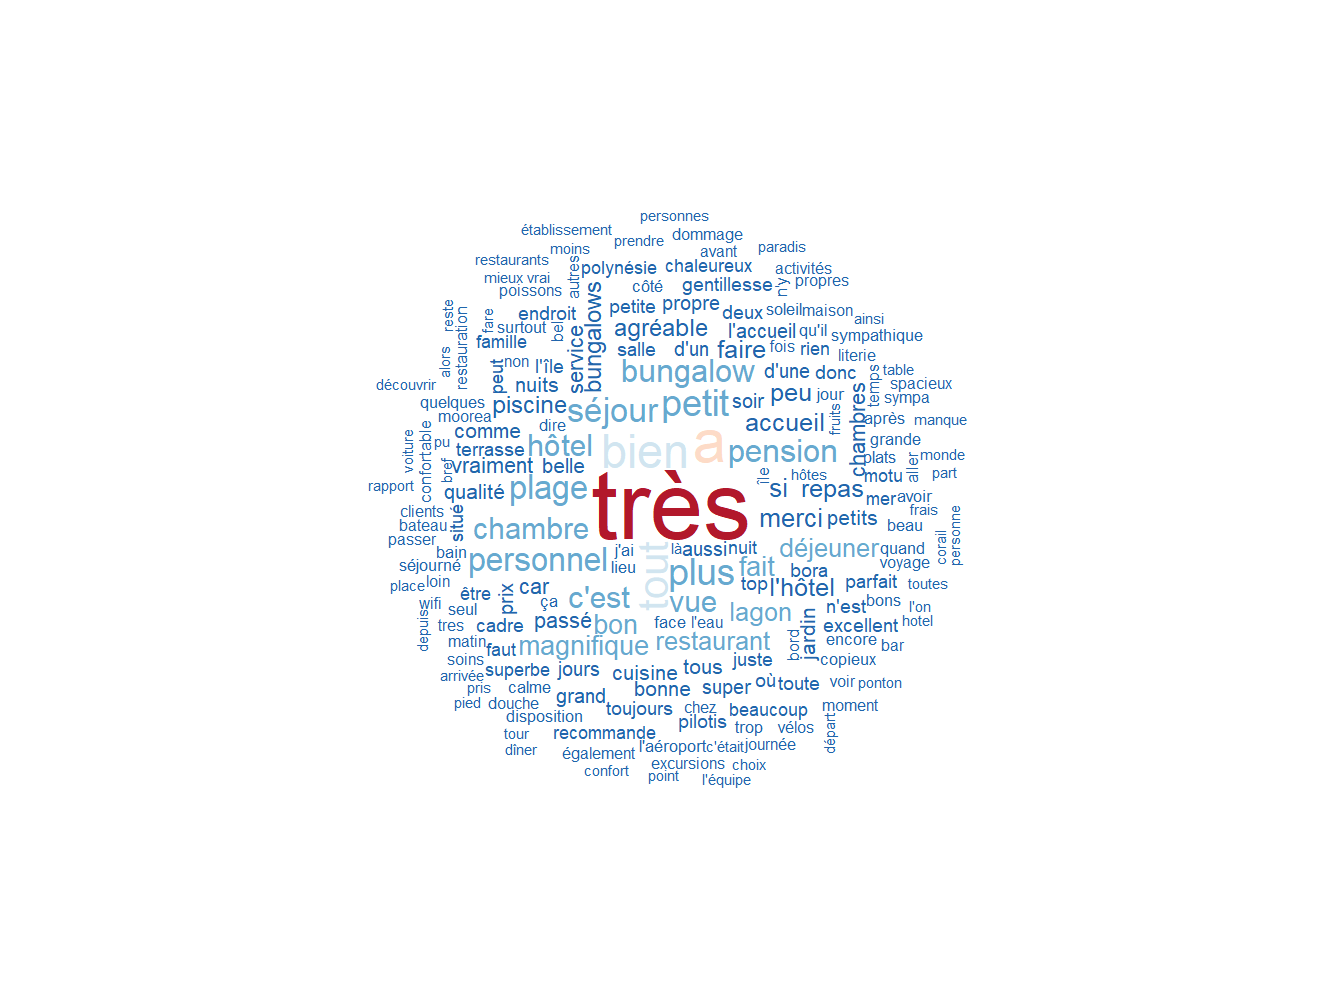
\includegraphics[width=0.8\linewidth]{bookdown-demo_files/figure-latex/508-1} 

}

\caption{Mots les plus fréquents du corpus}\label{fig:508}
\end{figure}

\hypertarget{identifier-les-noms-propres}{%
\subsection{Identifier les noms propres}\label{identifier-les-noms-propres}}

On cherche ici à identifier les noms propres présents dans le corpus.

\begin{Shaded}
\begin{Highlighting}[]
\CommentTok{#on sélectionne les mots commençant par une majuscule}
\NormalTok{toks_cap <-}\StringTok{ }\KeywordTok{tokens_select}\NormalTok{(tok, }
                               \DataTypeTok{pattern =} \StringTok{"^[A-Z]"}\NormalTok{,}
                               \DataTypeTok{valuetype =} \StringTok{"regex"}\NormalTok{,}
                               \DataTypeTok{case_insensitive =} \OtherTok{FALSE}\NormalTok{, }
                               \DataTypeTok{padding =} \OtherTok{TRUE}\NormalTok{)}

\CommentTok{#on cherche les collocations}
\NormalTok{tstat_col_cap <-}\StringTok{ }\KeywordTok{textstat_collocations}\NormalTok{(toks_cap, }\DataTypeTok{min_count =} \DecValTok{3}\NormalTok{, }\DataTypeTok{tolower =} \OtherTok{FALSE}\NormalTok{)}
\KeywordTok{flextable}\NormalTok{(}\KeywordTok{head}\NormalTok{(}\KeywordTok{as.data.frame}\NormalTok{(tstat_col_cap)))}
\end{Highlighting}
\end{Shaded}

\providecommand{\docline}[3]{\noalign{\global\setlength{\arrayrulewidth}{#1}}\arrayrulecolor[HTML]{#2}\cline{#3}}

\setlength{\tabcolsep}{2pt}

\renewcommand*{\arraystretch}{1.5}

\begin{longtable}[c]{|p{0.75in}|p{0.75in}|p{0.75in}|p{0.75in}|p{0.75in}|p{0.75in}}



\hhline{>{\arrayrulecolor[HTML]{666666}\global\arrayrulewidth=2pt}->{\arrayrulecolor[HTML]{666666}\global\arrayrulewidth=2pt}->{\arrayrulecolor[HTML]{666666}\global\arrayrulewidth=2pt}->{\arrayrulecolor[HTML]{666666}\global\arrayrulewidth=2pt}->{\arrayrulecolor[HTML]{666666}\global\arrayrulewidth=2pt}->{\arrayrulecolor[HTML]{666666}\global\arrayrulewidth=2pt}-}

\multicolumn{1}{!{\color[HTML]{000000}\vrule width 0pt}>{\raggedright}p{\dimexpr 0.75in+0\tabcolsep+0\arrayrulewidth}}{\fontsize{11}{11}\selectfont{\textcolor[HTML]{000000}{\global\setmainfont{Arial}collocation}}} & \multicolumn{1}{!{\color[HTML]{000000}\vrule width 0pt}>{\raggedleft}p{\dimexpr 0.75in+0\tabcolsep+0\arrayrulewidth}}{\fontsize{11}{11}\selectfont{\textcolor[HTML]{000000}{\global\setmainfont{Arial}count}}} & \multicolumn{1}{!{\color[HTML]{000000}\vrule width 0pt}>{\raggedleft}p{\dimexpr 0.75in+0\tabcolsep+0\arrayrulewidth}}{\fontsize{11}{11}\selectfont{\textcolor[HTML]{000000}{\global\setmainfont{Arial}count\_nested}}} & \multicolumn{1}{!{\color[HTML]{000000}\vrule width 0pt}>{\raggedleft}p{\dimexpr 0.75in+0\tabcolsep+0\arrayrulewidth}}{\fontsize{11}{11}\selectfont{\textcolor[HTML]{000000}{\global\setmainfont{Arial}length}}} & \multicolumn{1}{!{\color[HTML]{000000}\vrule width 0pt}>{\raggedleft}p{\dimexpr 0.75in+0\tabcolsep+0\arrayrulewidth}}{\fontsize{11}{11}\selectfont{\textcolor[HTML]{000000}{\global\setmainfont{Arial}lambda}}} & \multicolumn{1}{!{\color[HTML]{000000}\vrule width 0pt}>{\raggedleft}p{\dimexpr 0.75in+0\tabcolsep+0\arrayrulewidth}!{\color[HTML]{000000}\vrule width 0pt}}{\fontsize{11}{11}\selectfont{\textcolor[HTML]{000000}{\global\setmainfont{Arial}z}}} \\

\noalign{\global\setlength{\arrayrulewidth}{2pt}}\arrayrulecolor[HTML]{666666}\cline{1-6}

\endfirsthead

\hhline{>{\arrayrulecolor[HTML]{666666}\global\arrayrulewidth=2pt}->{\arrayrulecolor[HTML]{666666}\global\arrayrulewidth=2pt}->{\arrayrulecolor[HTML]{666666}\global\arrayrulewidth=2pt}->{\arrayrulecolor[HTML]{666666}\global\arrayrulewidth=2pt}->{\arrayrulecolor[HTML]{666666}\global\arrayrulewidth=2pt}->{\arrayrulecolor[HTML]{666666}\global\arrayrulewidth=2pt}-}

\multicolumn{1}{!{\color[HTML]{000000}\vrule width 0pt}>{\raggedright}p{\dimexpr 0.75in+0\tabcolsep+0\arrayrulewidth}}{\fontsize{11}{11}\selectfont{\textcolor[HTML]{000000}{\global\setmainfont{Arial}collocation}}} & \multicolumn{1}{!{\color[HTML]{000000}\vrule width 0pt}>{\raggedleft}p{\dimexpr 0.75in+0\tabcolsep+0\arrayrulewidth}}{\fontsize{11}{11}\selectfont{\textcolor[HTML]{000000}{\global\setmainfont{Arial}count}}} & \multicolumn{1}{!{\color[HTML]{000000}\vrule width 0pt}>{\raggedleft}p{\dimexpr 0.75in+0\tabcolsep+0\arrayrulewidth}}{\fontsize{11}{11}\selectfont{\textcolor[HTML]{000000}{\global\setmainfont{Arial}count\_nested}}} & \multicolumn{1}{!{\color[HTML]{000000}\vrule width 0pt}>{\raggedleft}p{\dimexpr 0.75in+0\tabcolsep+0\arrayrulewidth}}{\fontsize{11}{11}\selectfont{\textcolor[HTML]{000000}{\global\setmainfont{Arial}length}}} & \multicolumn{1}{!{\color[HTML]{000000}\vrule width 0pt}>{\raggedleft}p{\dimexpr 0.75in+0\tabcolsep+0\arrayrulewidth}}{\fontsize{11}{11}\selectfont{\textcolor[HTML]{000000}{\global\setmainfont{Arial}lambda}}} & \multicolumn{1}{!{\color[HTML]{000000}\vrule width 0pt}>{\raggedleft}p{\dimexpr 0.75in+0\tabcolsep+0\arrayrulewidth}!{\color[HTML]{000000}\vrule width 0pt}}{\fontsize{11}{11}\selectfont{\textcolor[HTML]{000000}{\global\setmainfont{Arial}z}}} \\

\noalign{\global\setlength{\arrayrulewidth}{2pt}}\arrayrulecolor[HTML]{666666}\cline{1-6}\endhead



\multicolumn{1}{!{\color[HTML]{000000}\vrule width 0pt}>{\raggedright}p{\dimexpr 0.75in+0\tabcolsep+0\arrayrulewidth}}{\fontsize{11}{11}\selectfont{\textcolor[HTML]{000000}{\global\setmainfont{Arial}Bora\ Bora}}} & \multicolumn{1}{!{\color[HTML]{000000}\vrule width 0pt}>{\raggedleft}p{\dimexpr 0.75in+0\tabcolsep+0\arrayrulewidth}}{\fontsize{11}{11}\selectfont{\textcolor[HTML]{000000}{\global\setmainfont{Arial}155}}} & \multicolumn{1}{!{\color[HTML]{000000}\vrule width 0pt}>{\raggedleft}p{\dimexpr 0.75in+0\tabcolsep+0\arrayrulewidth}}{\fontsize{11}{11}\selectfont{\textcolor[HTML]{000000}{\global\setmainfont{Arial}0}}} & \multicolumn{1}{!{\color[HTML]{000000}\vrule width 0pt}>{\raggedleft}p{\dimexpr 0.75in+0\tabcolsep+0\arrayrulewidth}}{\fontsize{11}{11}\selectfont{\textcolor[HTML]{000000}{\global\setmainfont{Arial}2}}} & \multicolumn{1}{!{\color[HTML]{000000}\vrule width 0pt}>{\raggedleft}p{\dimexpr 0.75in+0\tabcolsep+0\arrayrulewidth}}{\fontsize{11}{11}\selectfont{\textcolor[HTML]{000000}{\global\setmainfont{Arial}7.159074}}} & \multicolumn{1}{!{\color[HTML]{000000}\vrule width 0pt}>{\raggedleft}p{\dimexpr 0.75in+0\tabcolsep+0\arrayrulewidth}!{\color[HTML]{000000}\vrule width 0pt}}{\fontsize{11}{11}\selectfont{\textcolor[HTML]{000000}{\global\setmainfont{Arial}57.75427}}} \\





\multicolumn{1}{!{\color[HTML]{000000}\vrule width 0pt}>{\raggedright}p{\dimexpr 0.75in+0\tabcolsep+0\arrayrulewidth}}{\fontsize{11}{11}\selectfont{\textcolor[HTML]{000000}{\global\setmainfont{Arial}Pearl\ Beach}}} & \multicolumn{1}{!{\color[HTML]{000000}\vrule width 0pt}>{\raggedleft}p{\dimexpr 0.75in+0\tabcolsep+0\arrayrulewidth}}{\fontsize{11}{11}\selectfont{\textcolor[HTML]{000000}{\global\setmainfont{Arial}13}}} & \multicolumn{1}{!{\color[HTML]{000000}\vrule width 0pt}>{\raggedleft}p{\dimexpr 0.75in+0\tabcolsep+0\arrayrulewidth}}{\fontsize{11}{11}\selectfont{\textcolor[HTML]{000000}{\global\setmainfont{Arial}0}}} & \multicolumn{1}{!{\color[HTML]{000000}\vrule width 0pt}>{\raggedleft}p{\dimexpr 0.75in+0\tabcolsep+0\arrayrulewidth}}{\fontsize{11}{11}\selectfont{\textcolor[HTML]{000000}{\global\setmainfont{Arial}2}}} & \multicolumn{1}{!{\color[HTML]{000000}\vrule width 0pt}>{\raggedleft}p{\dimexpr 0.75in+0\tabcolsep+0\arrayrulewidth}}{\fontsize{11}{11}\selectfont{\textcolor[HTML]{000000}{\global\setmainfont{Arial}8.592055}}} & \multicolumn{1}{!{\color[HTML]{000000}\vrule width 0pt}>{\raggedleft}p{\dimexpr 0.75in+0\tabcolsep+0\arrayrulewidth}!{\color[HTML]{000000}\vrule width 0pt}}{\fontsize{11}{11}\selectfont{\textcolor[HTML]{000000}{\global\setmainfont{Arial}23.25054}}} \\





\multicolumn{1}{!{\color[HTML]{000000}\vrule width 0pt}>{\raggedright}p{\dimexpr 0.75in+0\tabcolsep+0\arrayrulewidth}}{\fontsize{11}{11}\selectfont{\textcolor[HTML]{000000}{\global\setmainfont{Arial}Jean\ Claude}}} & \multicolumn{1}{!{\color[HTML]{000000}\vrule width 0pt}>{\raggedleft}p{\dimexpr 0.75in+0\tabcolsep+0\arrayrulewidth}}{\fontsize{11}{11}\selectfont{\textcolor[HTML]{000000}{\global\setmainfont{Arial}13}}} & \multicolumn{1}{!{\color[HTML]{000000}\vrule width 0pt}>{\raggedleft}p{\dimexpr 0.75in+0\tabcolsep+0\arrayrulewidth}}{\fontsize{11}{11}\selectfont{\textcolor[HTML]{000000}{\global\setmainfont{Arial}0}}} & \multicolumn{1}{!{\color[HTML]{000000}\vrule width 0pt}>{\raggedleft}p{\dimexpr 0.75in+0\tabcolsep+0\arrayrulewidth}}{\fontsize{11}{11}\selectfont{\textcolor[HTML]{000000}{\global\setmainfont{Arial}2}}} & \multicolumn{1}{!{\color[HTML]{000000}\vrule width 0pt}>{\raggedleft}p{\dimexpr 0.75in+0\tabcolsep+0\arrayrulewidth}}{\fontsize{11}{11}\selectfont{\textcolor[HTML]{000000}{\global\setmainfont{Arial}8.980729}}} & \multicolumn{1}{!{\color[HTML]{000000}\vrule width 0pt}>{\raggedleft}p{\dimexpr 0.75in+0\tabcolsep+0\arrayrulewidth}!{\color[HTML]{000000}\vrule width 0pt}}{\fontsize{11}{11}\selectfont{\textcolor[HTML]{000000}{\global\setmainfont{Arial}22.41189}}} \\





\multicolumn{1}{!{\color[HTML]{000000}\vrule width 0pt}>{\raggedright}p{\dimexpr 0.75in+0\tabcolsep+0\arrayrulewidth}}{\fontsize{11}{11}\selectfont{\textcolor[HTML]{000000}{\global\setmainfont{Arial}Tiputa\ Lodge}}} & \multicolumn{1}{!{\color[HTML]{000000}\vrule width 0pt}>{\raggedleft}p{\dimexpr 0.75in+0\tabcolsep+0\arrayrulewidth}}{\fontsize{11}{11}\selectfont{\textcolor[HTML]{000000}{\global\setmainfont{Arial}13}}} & \multicolumn{1}{!{\color[HTML]{000000}\vrule width 0pt}>{\raggedleft}p{\dimexpr 0.75in+0\tabcolsep+0\arrayrulewidth}}{\fontsize{11}{11}\selectfont{\textcolor[HTML]{000000}{\global\setmainfont{Arial}0}}} & \multicolumn{1}{!{\color[HTML]{000000}\vrule width 0pt}>{\raggedleft}p{\dimexpr 0.75in+0\tabcolsep+0\arrayrulewidth}}{\fontsize{11}{11}\selectfont{\textcolor[HTML]{000000}{\global\setmainfont{Arial}2}}} & \multicolumn{1}{!{\color[HTML]{000000}\vrule width 0pt}>{\raggedleft}p{\dimexpr 0.75in+0\tabcolsep+0\arrayrulewidth}}{\fontsize{11}{11}\selectfont{\textcolor[HTML]{000000}{\global\setmainfont{Arial}7.129103}}} & \multicolumn{1}{!{\color[HTML]{000000}\vrule width 0pt}>{\raggedleft}p{\dimexpr 0.75in+0\tabcolsep+0\arrayrulewidth}!{\color[HTML]{000000}\vrule width 0pt}}{\fontsize{11}{11}\selectfont{\textcolor[HTML]{000000}{\global\setmainfont{Arial}22.06886}}} \\





\multicolumn{1}{!{\color[HTML]{000000}\vrule width 0pt}>{\raggedright}p{\dimexpr 0.75in+0\tabcolsep+0\arrayrulewidth}}{\fontsize{11}{11}\selectfont{\textcolor[HTML]{000000}{\global\setmainfont{Arial}Taha'a\ Island}}} & \multicolumn{1}{!{\color[HTML]{000000}\vrule width 0pt}>{\raggedleft}p{\dimexpr 0.75in+0\tabcolsep+0\arrayrulewidth}}{\fontsize{11}{11}\selectfont{\textcolor[HTML]{000000}{\global\setmainfont{Arial}10}}} & \multicolumn{1}{!{\color[HTML]{000000}\vrule width 0pt}>{\raggedleft}p{\dimexpr 0.75in+0\tabcolsep+0\arrayrulewidth}}{\fontsize{11}{11}\selectfont{\textcolor[HTML]{000000}{\global\setmainfont{Arial}0}}} & \multicolumn{1}{!{\color[HTML]{000000}\vrule width 0pt}>{\raggedleft}p{\dimexpr 0.75in+0\tabcolsep+0\arrayrulewidth}}{\fontsize{11}{11}\selectfont{\textcolor[HTML]{000000}{\global\setmainfont{Arial}2}}} & \multicolumn{1}{!{\color[HTML]{000000}\vrule width 0pt}>{\raggedleft}p{\dimexpr 0.75in+0\tabcolsep+0\arrayrulewidth}}{\fontsize{11}{11}\selectfont{\textcolor[HTML]{000000}{\global\setmainfont{Arial}8.272921}}} & \multicolumn{1}{!{\color[HTML]{000000}\vrule width 0pt}>{\raggedleft}p{\dimexpr 0.75in+0\tabcolsep+0\arrayrulewidth}!{\color[HTML]{000000}\vrule width 0pt}}{\fontsize{11}{11}\selectfont{\textcolor[HTML]{000000}{\global\setmainfont{Arial}20.98451}}} \\





\multicolumn{1}{!{\color[HTML]{000000}\vrule width 0pt}>{\raggedright}p{\dimexpr 0.75in+0\tabcolsep+0\arrayrulewidth}}{\fontsize{11}{11}\selectfont{\textcolor[HTML]{000000}{\global\setmainfont{Arial}Nuku\ Hiva}}} & \multicolumn{1}{!{\color[HTML]{000000}\vrule width 0pt}>{\raggedleft}p{\dimexpr 0.75in+0\tabcolsep+0\arrayrulewidth}}{\fontsize{11}{11}\selectfont{\textcolor[HTML]{000000}{\global\setmainfont{Arial}23}}} & \multicolumn{1}{!{\color[HTML]{000000}\vrule width 0pt}>{\raggedleft}p{\dimexpr 0.75in+0\tabcolsep+0\arrayrulewidth}}{\fontsize{11}{11}\selectfont{\textcolor[HTML]{000000}{\global\setmainfont{Arial}0}}} & \multicolumn{1}{!{\color[HTML]{000000}\vrule width 0pt}>{\raggedleft}p{\dimexpr 0.75in+0\tabcolsep+0\arrayrulewidth}}{\fontsize{11}{11}\selectfont{\textcolor[HTML]{000000}{\global\setmainfont{Arial}2}}} & \multicolumn{1}{!{\color[HTML]{000000}\vrule width 0pt}>{\raggedleft}p{\dimexpr 0.75in+0\tabcolsep+0\arrayrulewidth}}{\fontsize{11}{11}\selectfont{\textcolor[HTML]{000000}{\global\setmainfont{Arial}11.619165}}} & \multicolumn{1}{!{\color[HTML]{000000}\vrule width 0pt}>{\raggedleft}p{\dimexpr 0.75in+0\tabcolsep+0\arrayrulewidth}!{\color[HTML]{000000}\vrule width 0pt}}{\fontsize{11}{11}\selectfont{\textcolor[HTML]{000000}{\global\setmainfont{Arial}20.66761}}} \\

\noalign{\global\setlength{\arrayrulewidth}{2pt}}\arrayrulecolor[HTML]{666666}\cline{1-6}

\end{longtable}

\hypertarget{composer-des-tokens-uxe0-partir-dexpressions-multi-mots}{%
\subsection{\texorpdfstring{Composer des \emph{tokens} à partir d'expressions multi-mots}{Composer des tokens à partir d'expressions multi-mots}}\label{composer-des-tokens-uxe0-partir-dexpressions-multi-mots}}

Dans ce corpus, les noms propres correspondent aux noms des îles et des hôtels, et aux prénoms composés. La valeur du lambda montre la force de l'association entre les mots, on retiendra d'une manière générale un lambda au moins supérieur à 3 pour remplacer les \emph{tokens} d'origine par leurs n-grammes.

\begin{Shaded}
\begin{Highlighting}[]
\NormalTok{toks_comp <-}\StringTok{ }\KeywordTok{tokens_compound}\NormalTok{(tok, }\DataTypeTok{pattern =}\NormalTok{ tstat_col_cap[tstat_col_cap}\OperatorTok{$}\NormalTok{z }\OperatorTok{>}\StringTok{ }\DecValTok{3}\NormalTok{], }
                             \DataTypeTok{case_insensitive =} \OtherTok{FALSE}\NormalTok{)}

\KeywordTok{head}\NormalTok{(toks_comp)}
\end{Highlighting}
\end{Shaded}

\begin{verbatim}
## Tokens consisting of 6 documents and 21 docvars.
## 1 :
##  [1] "Tout"       ""           "magnifique" ""           "Vahine"    
##  [6] "island"     "Séjour"     ""           "rêve"       ""          
## [11] ""           "équipe"    
## [ ... and 22 more ]
## 
## 2 :
##  [1] "Tout"         ""             "parfait"      ""             "meilleure"   
##  [6] "expérience"   ""             "plus"         "belle"        "découverte"  
## [11] ""             "Polynésie.Un"
## [ ... and 37 more ]
## 
## 3 :
##  [1] ""                "séjour"          "magnifique"      "jours"          
##  [5] "époustouflants"  "accueillis"      "chaleureusement" ""               
##  [9] "toute"           "l'équipe"        ""                "Vahine_Island"  
## [ ... and 26 more ]
## 
## 4 :
##  [1] "Vraiment"    "beau"        "cadre"       "idyllique"   "personnel"  
##  [6] "très"        "attentionné" ""            ""            "adoré"      
## [11] ""            "séjour"     
## [ ... and 27 more ]
## 
## 5 :
##  [1] ""              "Vahiné_Island" ""              "entre"        
##  [5] ""              ""              "monde"         "parallèle"    
##  [9] "où"            ""              ""              "sait"         
## [ ... and 125 more ]
## 
## 6 :
##  [1] ""              ""              "adoré"         ""             
##  [5] "séjour"        ""              "Vahiné_Island" ""             
##  [9] ""              "enfants"       "bungalow"      ""             
## [ ... and 76 more ]
\end{verbatim}

\begin{Shaded}
\begin{Highlighting}[]
\NormalTok{dfm<-}\KeywordTok{dfm}\NormalTok{(toks_comp, }\DataTypeTok{remove_padding=}\OtherTok{TRUE}\NormalTok{)}
\KeywordTok{textplot_wordcloud}\NormalTok{(dfm, }\DataTypeTok{max_words =} \DecValTok{200}\NormalTok{, }\DataTypeTok{color =} \KeywordTok{rev}\NormalTok{(RColorBrewer}\OperatorTok{::}\KeywordTok{brewer.pal}\NormalTok{(}\DecValTok{6}\NormalTok{, }\StringTok{"RdBu"}\NormalTok{)))}
\end{Highlighting}
\end{Shaded}

\begin{figure}

{\centering 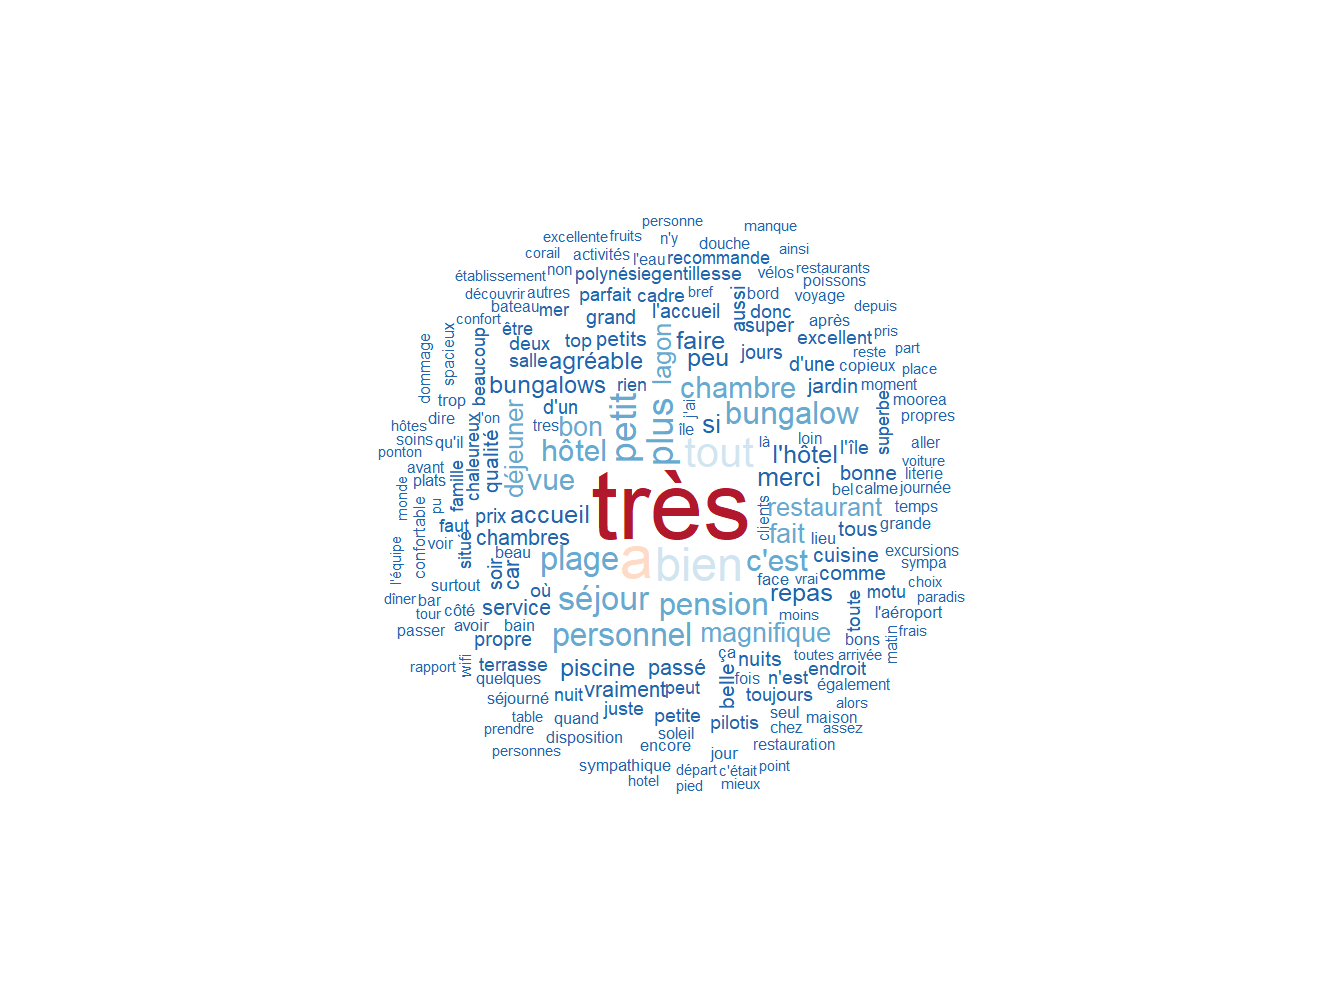
\includegraphics[width=0.8\linewidth]{bookdown-demo_files/figure-latex/510-1} 

}

\caption{Mots les plus fréquents du corpus}\label{fig:510}
\end{figure}

\hypertarget{identifier-les-autres-concepts}{%
\subsection{Identifier les autres concepts}\label{identifier-les-autres-concepts}}

Dans ce corpus, on peut aussi s'attendre à voir apparaître d'autres expressions multi-mots qui représentent des concepts, telles que ``petit déjeuner''.

\begin{Shaded}
\begin{Highlighting}[]
\NormalTok{col<-}\KeywordTok{textstat_collocations}\NormalTok{(toks_comp, }\DataTypeTok{min_count =} \DecValTok{10}\NormalTok{)}

\KeywordTok{flextable}\NormalTok{(}\KeywordTok{head}\NormalTok{(}\KeywordTok{as.data.frame}\NormalTok{(col)))}
\end{Highlighting}
\end{Shaded}

\providecommand{\docline}[3]{\noalign{\global\setlength{\arrayrulewidth}{#1}}\arrayrulecolor[HTML]{#2}\cline{#3}}

\setlength{\tabcolsep}{2pt}

\renewcommand*{\arraystretch}{1.5}

\begin{longtable}[c]{|p{0.75in}|p{0.75in}|p{0.75in}|p{0.75in}|p{0.75in}|p{0.75in}}



\hhline{>{\arrayrulecolor[HTML]{666666}\global\arrayrulewidth=2pt}->{\arrayrulecolor[HTML]{666666}\global\arrayrulewidth=2pt}->{\arrayrulecolor[HTML]{666666}\global\arrayrulewidth=2pt}->{\arrayrulecolor[HTML]{666666}\global\arrayrulewidth=2pt}->{\arrayrulecolor[HTML]{666666}\global\arrayrulewidth=2pt}->{\arrayrulecolor[HTML]{666666}\global\arrayrulewidth=2pt}-}

\multicolumn{1}{!{\color[HTML]{000000}\vrule width 0pt}>{\raggedright}p{\dimexpr 0.75in+0\tabcolsep+0\arrayrulewidth}}{\fontsize{11}{11}\selectfont{\textcolor[HTML]{000000}{\global\setmainfont{Arial}collocation}}} & \multicolumn{1}{!{\color[HTML]{000000}\vrule width 0pt}>{\raggedleft}p{\dimexpr 0.75in+0\tabcolsep+0\arrayrulewidth}}{\fontsize{11}{11}\selectfont{\textcolor[HTML]{000000}{\global\setmainfont{Arial}count}}} & \multicolumn{1}{!{\color[HTML]{000000}\vrule width 0pt}>{\raggedleft}p{\dimexpr 0.75in+0\tabcolsep+0\arrayrulewidth}}{\fontsize{11}{11}\selectfont{\textcolor[HTML]{000000}{\global\setmainfont{Arial}count\_nested}}} & \multicolumn{1}{!{\color[HTML]{000000}\vrule width 0pt}>{\raggedleft}p{\dimexpr 0.75in+0\tabcolsep+0\arrayrulewidth}}{\fontsize{11}{11}\selectfont{\textcolor[HTML]{000000}{\global\setmainfont{Arial}length}}} & \multicolumn{1}{!{\color[HTML]{000000}\vrule width 0pt}>{\raggedleft}p{\dimexpr 0.75in+0\tabcolsep+0\arrayrulewidth}}{\fontsize{11}{11}\selectfont{\textcolor[HTML]{000000}{\global\setmainfont{Arial}lambda}}} & \multicolumn{1}{!{\color[HTML]{000000}\vrule width 0pt}>{\raggedleft}p{\dimexpr 0.75in+0\tabcolsep+0\arrayrulewidth}!{\color[HTML]{000000}\vrule width 0pt}}{\fontsize{11}{11}\selectfont{\textcolor[HTML]{000000}{\global\setmainfont{Arial}z}}} \\

\noalign{\global\setlength{\arrayrulewidth}{2pt}}\arrayrulecolor[HTML]{666666}\cline{1-6}

\endfirsthead

\hhline{>{\arrayrulecolor[HTML]{666666}\global\arrayrulewidth=2pt}->{\arrayrulecolor[HTML]{666666}\global\arrayrulewidth=2pt}->{\arrayrulecolor[HTML]{666666}\global\arrayrulewidth=2pt}->{\arrayrulecolor[HTML]{666666}\global\arrayrulewidth=2pt}->{\arrayrulecolor[HTML]{666666}\global\arrayrulewidth=2pt}->{\arrayrulecolor[HTML]{666666}\global\arrayrulewidth=2pt}-}

\multicolumn{1}{!{\color[HTML]{000000}\vrule width 0pt}>{\raggedright}p{\dimexpr 0.75in+0\tabcolsep+0\arrayrulewidth}}{\fontsize{11}{11}\selectfont{\textcolor[HTML]{000000}{\global\setmainfont{Arial}collocation}}} & \multicolumn{1}{!{\color[HTML]{000000}\vrule width 0pt}>{\raggedleft}p{\dimexpr 0.75in+0\tabcolsep+0\arrayrulewidth}}{\fontsize{11}{11}\selectfont{\textcolor[HTML]{000000}{\global\setmainfont{Arial}count}}} & \multicolumn{1}{!{\color[HTML]{000000}\vrule width 0pt}>{\raggedleft}p{\dimexpr 0.75in+0\tabcolsep+0\arrayrulewidth}}{\fontsize{11}{11}\selectfont{\textcolor[HTML]{000000}{\global\setmainfont{Arial}count\_nested}}} & \multicolumn{1}{!{\color[HTML]{000000}\vrule width 0pt}>{\raggedleft}p{\dimexpr 0.75in+0\tabcolsep+0\arrayrulewidth}}{\fontsize{11}{11}\selectfont{\textcolor[HTML]{000000}{\global\setmainfont{Arial}length}}} & \multicolumn{1}{!{\color[HTML]{000000}\vrule width 0pt}>{\raggedleft}p{\dimexpr 0.75in+0\tabcolsep+0\arrayrulewidth}}{\fontsize{11}{11}\selectfont{\textcolor[HTML]{000000}{\global\setmainfont{Arial}lambda}}} & \multicolumn{1}{!{\color[HTML]{000000}\vrule width 0pt}>{\raggedleft}p{\dimexpr 0.75in+0\tabcolsep+0\arrayrulewidth}!{\color[HTML]{000000}\vrule width 0pt}}{\fontsize{11}{11}\selectfont{\textcolor[HTML]{000000}{\global\setmainfont{Arial}z}}} \\

\noalign{\global\setlength{\arrayrulewidth}{2pt}}\arrayrulecolor[HTML]{666666}\cline{1-6}\endhead



\multicolumn{1}{!{\color[HTML]{000000}\vrule width 0pt}>{\raggedright}p{\dimexpr 0.75in+0\tabcolsep+0\arrayrulewidth}}{\fontsize{11}{11}\selectfont{\textcolor[HTML]{000000}{\global\setmainfont{Arial}petit\ déjeuner}}} & \multicolumn{1}{!{\color[HTML]{000000}\vrule width 0pt}>{\raggedleft}p{\dimexpr 0.75in+0\tabcolsep+0\arrayrulewidth}}{\fontsize{11}{11}\selectfont{\textcolor[HTML]{000000}{\global\setmainfont{Arial}769}}} & \multicolumn{1}{!{\color[HTML]{000000}\vrule width 0pt}>{\raggedleft}p{\dimexpr 0.75in+0\tabcolsep+0\arrayrulewidth}}{\fontsize{11}{11}\selectfont{\textcolor[HTML]{000000}{\global\setmainfont{Arial}0}}} & \multicolumn{1}{!{\color[HTML]{000000}\vrule width 0pt}>{\raggedleft}p{\dimexpr 0.75in+0\tabcolsep+0\arrayrulewidth}}{\fontsize{11}{11}\selectfont{\textcolor[HTML]{000000}{\global\setmainfont{Arial}2}}} & \multicolumn{1}{!{\color[HTML]{000000}\vrule width 0pt}>{\raggedleft}p{\dimexpr 0.75in+0\tabcolsep+0\arrayrulewidth}}{\fontsize{11}{11}\selectfont{\textcolor[HTML]{000000}{\global\setmainfont{Arial}7.510485}}} & \multicolumn{1}{!{\color[HTML]{000000}\vrule width 0pt}>{\raggedleft}p{\dimexpr 0.75in+0\tabcolsep+0\arrayrulewidth}!{\color[HTML]{000000}\vrule width 0pt}}{\fontsize{11}{11}\selectfont{\textcolor[HTML]{000000}{\global\setmainfont{Arial}85.88487}}} \\





\multicolumn{1}{!{\color[HTML]{000000}\vrule width 0pt}>{\raggedright}p{\dimexpr 0.75in+0\tabcolsep+0\arrayrulewidth}}{\fontsize{11}{11}\selectfont{\textcolor[HTML]{000000}{\global\setmainfont{Arial}très\ bien}}} & \multicolumn{1}{!{\color[HTML]{000000}\vrule width 0pt}>{\raggedleft}p{\dimexpr 0.75in+0\tabcolsep+0\arrayrulewidth}}{\fontsize{11}{11}\selectfont{\textcolor[HTML]{000000}{\global\setmainfont{Arial}714}}} & \multicolumn{1}{!{\color[HTML]{000000}\vrule width 0pt}>{\raggedleft}p{\dimexpr 0.75in+0\tabcolsep+0\arrayrulewidth}}{\fontsize{11}{11}\selectfont{\textcolor[HTML]{000000}{\global\setmainfont{Arial}0}}} & \multicolumn{1}{!{\color[HTML]{000000}\vrule width 0pt}>{\raggedleft}p{\dimexpr 0.75in+0\tabcolsep+0\arrayrulewidth}}{\fontsize{11}{11}\selectfont{\textcolor[HTML]{000000}{\global\setmainfont{Arial}2}}} & \multicolumn{1}{!{\color[HTML]{000000}\vrule width 0pt}>{\raggedleft}p{\dimexpr 0.75in+0\tabcolsep+0\arrayrulewidth}}{\fontsize{11}{11}\selectfont{\textcolor[HTML]{000000}{\global\setmainfont{Arial}3.591647}}} & \multicolumn{1}{!{\color[HTML]{000000}\vrule width 0pt}>{\raggedleft}p{\dimexpr 0.75in+0\tabcolsep+0\arrayrulewidth}!{\color[HTML]{000000}\vrule width 0pt}}{\fontsize{11}{11}\selectfont{\textcolor[HTML]{000000}{\global\setmainfont{Arial}76.20326}}} \\





\multicolumn{1}{!{\color[HTML]{000000}\vrule width 0pt}>{\raggedright}p{\dimexpr 0.75in+0\tabcolsep+0\arrayrulewidth}}{\fontsize{11}{11}\selectfont{\textcolor[HTML]{000000}{\global\setmainfont{Arial}très\ bon}}} & \multicolumn{1}{!{\color[HTML]{000000}\vrule width 0pt}>{\raggedleft}p{\dimexpr 0.75in+0\tabcolsep+0\arrayrulewidth}}{\fontsize{11}{11}\selectfont{\textcolor[HTML]{000000}{\global\setmainfont{Arial}422}}} & \multicolumn{1}{!{\color[HTML]{000000}\vrule width 0pt}>{\raggedleft}p{\dimexpr 0.75in+0\tabcolsep+0\arrayrulewidth}}{\fontsize{11}{11}\selectfont{\textcolor[HTML]{000000}{\global\setmainfont{Arial}0}}} & \multicolumn{1}{!{\color[HTML]{000000}\vrule width 0pt}>{\raggedleft}p{\dimexpr 0.75in+0\tabcolsep+0\arrayrulewidth}}{\fontsize{11}{11}\selectfont{\textcolor[HTML]{000000}{\global\setmainfont{Arial}2}}} & \multicolumn{1}{!{\color[HTML]{000000}\vrule width 0pt}>{\raggedleft}p{\dimexpr 0.75in+0\tabcolsep+0\arrayrulewidth}}{\fontsize{11}{11}\selectfont{\textcolor[HTML]{000000}{\global\setmainfont{Arial}4.072595}}} & \multicolumn{1}{!{\color[HTML]{000000}\vrule width 0pt}>{\raggedleft}p{\dimexpr 0.75in+0\tabcolsep+0\arrayrulewidth}!{\color[HTML]{000000}\vrule width 0pt}}{\fontsize{11}{11}\selectfont{\textcolor[HTML]{000000}{\global\setmainfont{Arial}61.79011}}} \\





\multicolumn{1}{!{\color[HTML]{000000}\vrule width 0pt}>{\raggedright}p{\dimexpr 0.75in+0\tabcolsep+0\arrayrulewidth}}{\fontsize{11}{11}\selectfont{\textcolor[HTML]{000000}{\global\setmainfont{Arial}très\ agréable}}} & \multicolumn{1}{!{\color[HTML]{000000}\vrule width 0pt}>{\raggedleft}p{\dimexpr 0.75in+0\tabcolsep+0\arrayrulewidth}}{\fontsize{11}{11}\selectfont{\textcolor[HTML]{000000}{\global\setmainfont{Arial}374}}} & \multicolumn{1}{!{\color[HTML]{000000}\vrule width 0pt}>{\raggedleft}p{\dimexpr 0.75in+0\tabcolsep+0\arrayrulewidth}}{\fontsize{11}{11}\selectfont{\textcolor[HTML]{000000}{\global\setmainfont{Arial}0}}} & \multicolumn{1}{!{\color[HTML]{000000}\vrule width 0pt}>{\raggedleft}p{\dimexpr 0.75in+0\tabcolsep+0\arrayrulewidth}}{\fontsize{11}{11}\selectfont{\textcolor[HTML]{000000}{\global\setmainfont{Arial}2}}} & \multicolumn{1}{!{\color[HTML]{000000}\vrule width 0pt}>{\raggedleft}p{\dimexpr 0.75in+0\tabcolsep+0\arrayrulewidth}}{\fontsize{11}{11}\selectfont{\textcolor[HTML]{000000}{\global\setmainfont{Arial}4.200133}}} & \multicolumn{1}{!{\color[HTML]{000000}\vrule width 0pt}>{\raggedleft}p{\dimexpr 0.75in+0\tabcolsep+0\arrayrulewidth}!{\color[HTML]{000000}\vrule width 0pt}}{\fontsize{11}{11}\selectfont{\textcolor[HTML]{000000}{\global\setmainfont{Arial}58.42280}}} \\





\multicolumn{1}{!{\color[HTML]{000000}\vrule width 0pt}>{\raggedright}p{\dimexpr 0.75in+0\tabcolsep+0\arrayrulewidth}}{\fontsize{11}{11}\selectfont{\textcolor[HTML]{000000}{\global\setmainfont{Arial}grand\ merci}}} & \multicolumn{1}{!{\color[HTML]{000000}\vrule width 0pt}>{\raggedleft}p{\dimexpr 0.75in+0\tabcolsep+0\arrayrulewidth}}{\fontsize{11}{11}\selectfont{\textcolor[HTML]{000000}{\global\setmainfont{Arial}167}}} & \multicolumn{1}{!{\color[HTML]{000000}\vrule width 0pt}>{\raggedleft}p{\dimexpr 0.75in+0\tabcolsep+0\arrayrulewidth}}{\fontsize{11}{11}\selectfont{\textcolor[HTML]{000000}{\global\setmainfont{Arial}0}}} & \multicolumn{1}{!{\color[HTML]{000000}\vrule width 0pt}>{\raggedleft}p{\dimexpr 0.75in+0\tabcolsep+0\arrayrulewidth}}{\fontsize{11}{11}\selectfont{\textcolor[HTML]{000000}{\global\setmainfont{Arial}2}}} & \multicolumn{1}{!{\color[HTML]{000000}\vrule width 0pt}>{\raggedleft}p{\dimexpr 0.75in+0\tabcolsep+0\arrayrulewidth}}{\fontsize{11}{11}\selectfont{\textcolor[HTML]{000000}{\global\setmainfont{Arial}5.650650}}} & \multicolumn{1}{!{\color[HTML]{000000}\vrule width 0pt}>{\raggedleft}p{\dimexpr 0.75in+0\tabcolsep+0\arrayrulewidth}!{\color[HTML]{000000}\vrule width 0pt}}{\fontsize{11}{11}\selectfont{\textcolor[HTML]{000000}{\global\setmainfont{Arial}55.78169}}} \\





\multicolumn{1}{!{\color[HTML]{000000}\vrule width 0pt}>{\raggedright}p{\dimexpr 0.75in+0\tabcolsep+0\arrayrulewidth}}{\fontsize{11}{11}\selectfont{\textcolor[HTML]{000000}{\global\setmainfont{Arial}passé\ nuits}}} & \multicolumn{1}{!{\color[HTML]{000000}\vrule width 0pt}>{\raggedleft}p{\dimexpr 0.75in+0\tabcolsep+0\arrayrulewidth}}{\fontsize{11}{11}\selectfont{\textcolor[HTML]{000000}{\global\setmainfont{Arial}151}}} & \multicolumn{1}{!{\color[HTML]{000000}\vrule width 0pt}>{\raggedleft}p{\dimexpr 0.75in+0\tabcolsep+0\arrayrulewidth}}{\fontsize{11}{11}\selectfont{\textcolor[HTML]{000000}{\global\setmainfont{Arial}0}}} & \multicolumn{1}{!{\color[HTML]{000000}\vrule width 0pt}>{\raggedleft}p{\dimexpr 0.75in+0\tabcolsep+0\arrayrulewidth}}{\fontsize{11}{11}\selectfont{\textcolor[HTML]{000000}{\global\setmainfont{Arial}2}}} & \multicolumn{1}{!{\color[HTML]{000000}\vrule width 0pt}>{\raggedleft}p{\dimexpr 0.75in+0\tabcolsep+0\arrayrulewidth}}{\fontsize{11}{11}\selectfont{\textcolor[HTML]{000000}{\global\setmainfont{Arial}5.517906}}} & \multicolumn{1}{!{\color[HTML]{000000}\vrule width 0pt}>{\raggedleft}p{\dimexpr 0.75in+0\tabcolsep+0\arrayrulewidth}!{\color[HTML]{000000}\vrule width 0pt}}{\fontsize{11}{11}\selectfont{\textcolor[HTML]{000000}{\global\setmainfont{Arial}53.58480}}} \\

\noalign{\global\setlength{\arrayrulewidth}{2pt}}\arrayrulecolor[HTML]{666666}\cline{1-6}

\end{longtable}

Au vue de la diversité des collocations, on choisit un lambda supérieur à 7 pour retenir les concepts les plus pertinents.

\begin{Shaded}
\begin{Highlighting}[]
\NormalTok{toks_comp <-}\StringTok{ }\KeywordTok{tokens_compound}\NormalTok{(tok, }\DataTypeTok{pattern =}\NormalTok{ col[col}\OperatorTok{$}\NormalTok{z }\OperatorTok{>}\StringTok{ }\DecValTok{7}\NormalTok{])}

\KeywordTok{head}\NormalTok{(toks_comp)}
\end{Highlighting}
\end{Shaded}

\begin{verbatim}
## Tokens consisting of 6 documents and 21 docvars.
## 1 :
##  [1] "Tout"       ""           "magnifique" ""           "Vahine"    
##  [6] "island"     "Séjour"     ""           "rêve"       ""          
## [11] ""           "équipe"    
## [ ... and 22 more ]
## 
## 2 :
##  [1] "Tout"         ""             "parfait"      ""             "meilleure"   
##  [6] "expérience"   ""             "plus_belle"   "découverte"   ""            
## [11] "Polynésie.Un" "grand_merci" 
## [ ... and 33 more ]
## 
## 3 :
##  [1] ""                "séjour"          "magnifique"      "jours"          
##  [5] "époustouflants"  "accueillis"      "chaleureusement" ""               
##  [9] "toute_l'équipe"  ""                "Vahine"          "Island"         
## [ ... and 26 more ]
## 
## 4 :
##  [1] "Vraiment"                   "beau"                      
##  [3] "cadre_idyllique"            "personnel_très_attentionné"
##  [5] ""                           ""                          
##  [7] "adoré"                      ""                          
##  [9] "séjour"                     "attention"                 
## [11] "spéciale"                   ""                          
## [ ... and 22 more ]
## 
## 5 :
##  [1] ""          "Vahiné"    "Island"    ""          "entre"     ""         
##  [7] ""          "monde"     "parallèle" "où"        ""          ""         
## [ ... and 117 more ]
## 
## 6 :
##  [1] ""         ""         "adoré"    ""         "séjour"   ""        
##  [7] "Vahiné"   "Island"   ""         ""         "enfants"  "bungalow"
## [ ... and 74 more ]
\end{verbatim}

\begin{Shaded}
\begin{Highlighting}[]
\NormalTok{dfm<-}\KeywordTok{dfm}\NormalTok{(toks_comp, }\DataTypeTok{remove_padding=}\OtherTok{TRUE}\NormalTok{)}
\KeywordTok{textplot_wordcloud}\NormalTok{(dfm, }\DataTypeTok{max_words =} \DecValTok{200}\NormalTok{, }\DataTypeTok{color =} \KeywordTok{rev}\NormalTok{(RColorBrewer}\OperatorTok{::}\KeywordTok{brewer.pal}\NormalTok{(}\DecValTok{6}\NormalTok{, }\StringTok{"RdBu"}\NormalTok{)))}
\end{Highlighting}
\end{Shaded}

\begin{figure}

{\centering 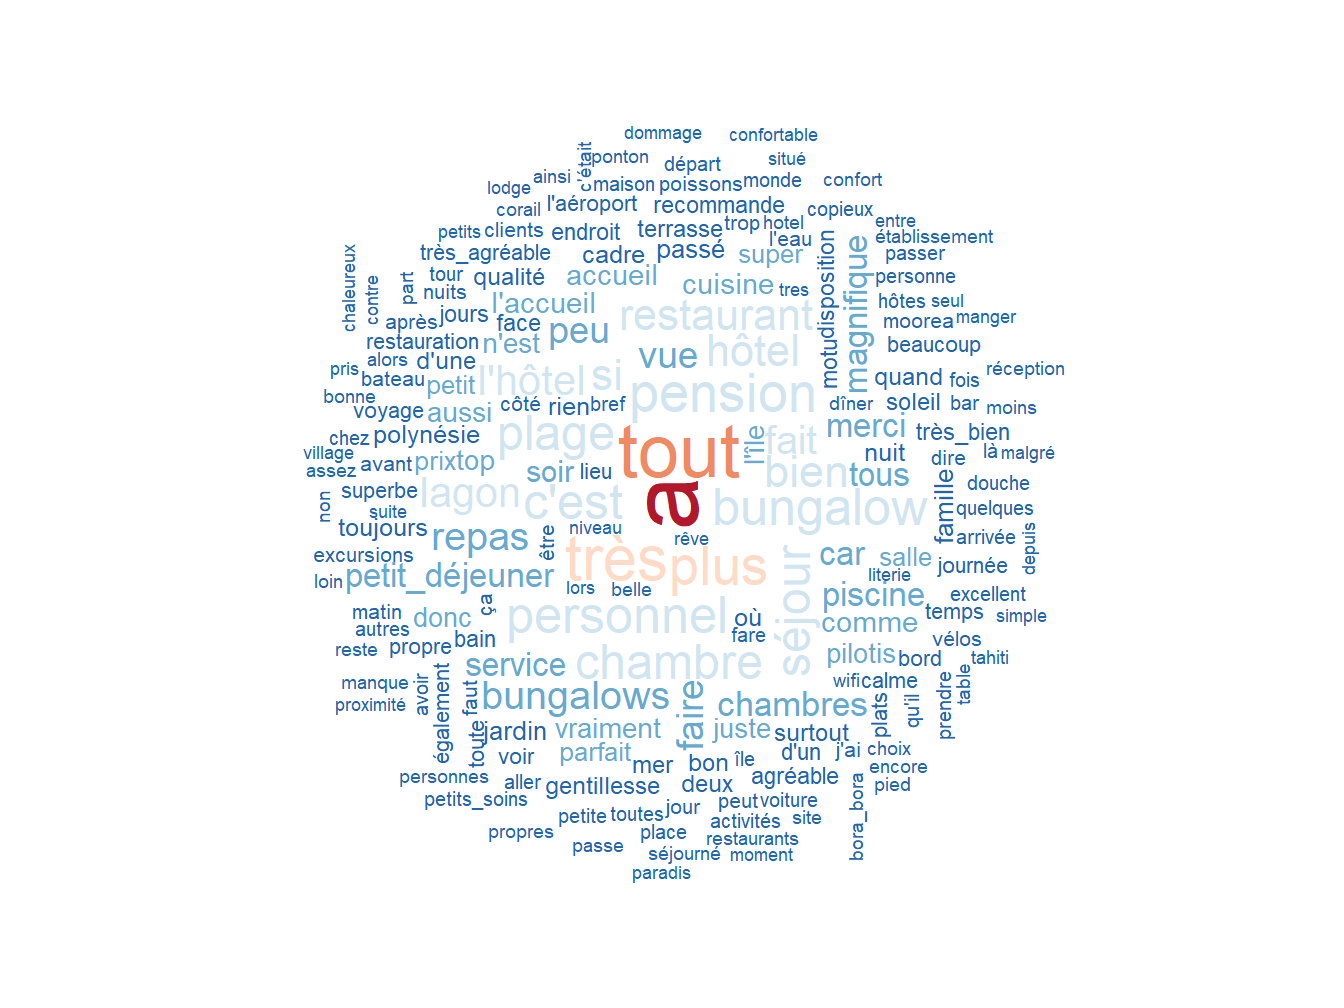
\includegraphics[width=0.8\linewidth]{bookdown-demo_files/figure-latex/512-1} 

}

\caption{Mots les plus fréquents du corpus}\label{fig:512}
\end{figure}

\hypertarget{conclusion-3}{%
\section{Conclusion}\label{conclusion-3}}

Dans ce chapitre, nous avons vu comment découper un corpus en unités, les \emph{tokens}. Nous avons abordé le sujet des n-grammes, et vu comment composer des \emph{tokens} à partir de concepts multi-mots, identifiés par des n-grammes adjacents.

\hypertarget{annot}{%
\chapter{Annotations lexicales et syntaxiques}\label{annot}}

Pour aller au-delà de l'analyse du seul lexique et de l'analyse de la cooccurence des termes à travers les textes, comme le font les méthodes de typologie et d'analyse factorielle des correspondance depuis longtemps, il est néçessaire d'analyser le texte en tenant compte de ses propriétés syntaxiques. Depuis une dizaine d'années, des outils puissants, les annotateurs, sont proposés de manière accessible.

Les plus connus sont Spacy, Stanford NLP et désormais UDpipe.

Dans l'environnement r différentes ressources sont disponibles : Quanteda, clean\_nlp, Udpipe, \ldots{}

Ils sont disponibles désormais dans de nombreuses langues même si la richesse et la précision obtenues varient d'une langue à l'autres

Ils s'appuient sur des corpus plus ou moins étendus et spécialisés d'annotations manuelle : les Treebanks.

Ils réalisent souvent plusieurs tâches dont les principales sont les suivantes :

\begin{itemize}
\tightlist
\item
  Tokeniser
\item
  Lemmatiser
\item
  Identifier les parts of speech
\item
  Identifier les dépendances syntaxiques
\item
  Identifier les entités nommées.
\item
  identifier les co-reférence
\end{itemize}

\hypertarget{tokenization}{%
\section{Tokenization}\label{tokenization}}

\hypertarget{les-niveaux-de-tokenisation}{%
\subsection{Les niveaux de tokenisation}\label{les-niveaux-de-tokenisation}}

Un token est une unité d'analyse dont la granularité est plus ou moins fine

\begin{itemize}
\tightlist
\item
  Le paragraphe est sans l'unité l'unité la plus générale, quand un texte est correctement rédigé, un paragraphe développe une idée.
\item
  La phrase est l'unité de langage, lui correpond un argument, une proposition. L'usage du point suivi d'un espace est assez général pour les identifier. C'est l'objet de tokenizers qui feront mieux en analysant le contexte de la phrase pour décider plus précisément si le point sépare bien deux phrase distinctes. Cette unité de phrase elle essentielle.
\item
  Le mot est la fois le niveau le plus évident et le plus courant.
\item
  On peut aussi souhaiter extraire d'un mot les suffixe et préfixe
\item
  On peut pour certains problème descendre au niveau de la syllabe et donc du phonème.
\item
  La lettre reste l'unité insécable.
\end{itemize}

\hypertarget{un-exemple-en-tidytext}{%
\subsection{Un exemple en tidytext}\label{un-exemple-en-tidytext}}

\hypertarget{stemmatisation-lemmatisation-et-synonymisation}{%
\section{Stemmatisation, lemmatisation et synonymisation}\label{stemmatisation-lemmatisation-et-synonymisation}}

Les mots prennent des formes variées, il peut être intéressant dans certains cas de réduire cette variété et ne considérer que l'idée des mots. Deux techniques sont disponibles

\hypertarget{la-stemmatisation}{%
\subsection{la stemmatisation}\label{la-stemmatisation}}

c'est un

\hypertarget{la-lemmatisation}{%
\subsection{la lemmatisation}\label{la-lemmatisation}}

Un lemme est un mot racine, sans inflexions de genre, de nombre ou de conjugaison. C'est généralement celui qu'on trouve dans les dictionnaire.

\hypertarget{synonymisation}{%
\subsection{Synonymisation}\label{synonymisation}}

le cas de wordnet et l'invention des synset

synonymes, antonymes, hipponyne, hyperonymes\ldots..

\url{https://cran.r-project.org/web/packages/wordnet/vignettes/wordnet.pdf}

\hypertarget{part-of-speech-pos}{%
\section{Part of Speech (POS)}\label{part-of-speech-pos}}

Dans une phrase les mots n'on pas la même valeur. Certains sont des nombres propres, ils se réfèrent à ce que nous venons de voir, c'est à dire des entitées nommées, d'autres désignent des catégories d'objet. Ce sont les noms communs qui se rapportent à des catégories de choses. Un marteau - si j'en avais un - peut être n'importe quel marteau, la masse qui casse la pierre, ou ce petit marteau qui me permet d'enfoncer un clou dans le cadre du tableau.

Des typologies universelles ont été construites, elles recouvrent des typologies plus spécifiques à certaines langues. Les désinences du latin ont par exemple disparu du français. Cette forme est spécifiques au latin, on la retrouvera en allemand. La notion de morphosntaxique désigne présisément que les variations de formes des mots dépendent d'une règle syntaxique. Prenons le verbe, et sa forme, ``être'', dont la forme au passé simple est ``était''. La forme des mots change, mais l'idée reste.

Une catégorisation en 17 éléments est proposée. En voici les \href{https://universaldependencies.org/u/pos/}{éléments et les définitions}

Un petit exemple avec le package \texttt{UDpipe}.

\begin{Shaded}
\begin{Highlighting}[]
\KeywordTok{library}\NormalTok{(udpipe)}
\NormalTok{fr <-}\StringTok{ }\KeywordTok{udpipe_download_model}\NormalTok{(}\DataTypeTok{language =} \StringTok{"french"}\NormalTok{)}
\NormalTok{udmodel_french <-}\StringTok{ }\KeywordTok{udpipe_load_model}\NormalTok{(}\DataTypeTok{file =} \StringTok{"french-gsd-ud-2.5-191206.udpipe"}\NormalTok{)}
\NormalTok{Citations <-}\StringTok{ }\KeywordTok{read_csv}\NormalTok{(}\StringTok{"./data/Citations.csv"}\NormalTok{)}

\NormalTok{Flaubert<-Citations }\OperatorTok
\StringTok{  }\KeywordTok{filter}\NormalTok{(doc}\OperatorTok{==}\DecValTok{1}\NormalTok{)}

\NormalTok{UD <-}\StringTok{ }\KeywordTok{udpipe_annotate}\NormalTok{(udmodel_french, }\DataTypeTok{x=}\NormalTok{Flaubert}\OperatorTok{$}\NormalTok{text)}
\NormalTok{x <-}\StringTok{ }\KeywordTok{as.data.frame}\NormalTok{(UD)}
\NormalTok{foo<-x }\OperatorTok\StringTok{ }
\StringTok{  }\KeywordTok{select}\NormalTok{(doc_id,paragraph_id, sentence_id, token_id,token,lemma,head_token_id, upos,feats)}\OperatorTok\KeywordTok{filter}\NormalTok{(sentence_id}\OperatorTok{==}\DecValTok{1}\NormalTok{)}
\KeywordTok{flextable}\NormalTok{(foo)}
\end{Highlighting}
\end{Shaded}

\providecommand{\docline}[3]{\noalign{\global\setlength{\arrayrulewidth}{#1}}\arrayrulecolor[HTML]{#2}\cline{#3}}

\setlength{\tabcolsep}{2pt}

\renewcommand*{\arraystretch}{1.5}

\begin{longtable}[c]{|p{0.75in}|p{0.75in}|p{0.75in}|p{0.75in}|p{0.75in}|p{0.75in}|p{0.75in}|p{0.75in}|p{0.75in}}



\hhline{>{\arrayrulecolor[HTML]{666666}\global\arrayrulewidth=2pt}->{\arrayrulecolor[HTML]{666666}\global\arrayrulewidth=2pt}->{\arrayrulecolor[HTML]{666666}\global\arrayrulewidth=2pt}->{\arrayrulecolor[HTML]{666666}\global\arrayrulewidth=2pt}->{\arrayrulecolor[HTML]{666666}\global\arrayrulewidth=2pt}->{\arrayrulecolor[HTML]{666666}\global\arrayrulewidth=2pt}->{\arrayrulecolor[HTML]{666666}\global\arrayrulewidth=2pt}->{\arrayrulecolor[HTML]{666666}\global\arrayrulewidth=2pt}->{\arrayrulecolor[HTML]{666666}\global\arrayrulewidth=2pt}-}

\multicolumn{1}{!{\color[HTML]{000000}\vrule width 0pt}>{\raggedright}p{\dimexpr 0.75in+0\tabcolsep+0\arrayrulewidth}}{\fontsize{11}{11}\selectfont{\textcolor[HTML]{000000}{\global\setmainfont{Arial}doc\_id}}} & \multicolumn{1}{!{\color[HTML]{000000}\vrule width 0pt}>{\raggedleft}p{\dimexpr 0.75in+0\tabcolsep+0\arrayrulewidth}}{\fontsize{11}{11}\selectfont{\textcolor[HTML]{000000}{\global\setmainfont{Arial}paragraph\_id}}} & \multicolumn{1}{!{\color[HTML]{000000}\vrule width 0pt}>{\raggedleft}p{\dimexpr 0.75in+0\tabcolsep+0\arrayrulewidth}}{\fontsize{11}{11}\selectfont{\textcolor[HTML]{000000}{\global\setmainfont{Arial}sentence\_id}}} & \multicolumn{1}{!{\color[HTML]{000000}\vrule width 0pt}>{\raggedright}p{\dimexpr 0.75in+0\tabcolsep+0\arrayrulewidth}}{\fontsize{11}{11}\selectfont{\textcolor[HTML]{000000}{\global\setmainfont{Arial}token\_id}}} & \multicolumn{1}{!{\color[HTML]{000000}\vrule width 0pt}>{\raggedright}p{\dimexpr 0.75in+0\tabcolsep+0\arrayrulewidth}}{\fontsize{11}{11}\selectfont{\textcolor[HTML]{000000}{\global\setmainfont{Arial}token}}} & \multicolumn{1}{!{\color[HTML]{000000}\vrule width 0pt}>{\raggedright}p{\dimexpr 0.75in+0\tabcolsep+0\arrayrulewidth}}{\fontsize{11}{11}\selectfont{\textcolor[HTML]{000000}{\global\setmainfont{Arial}lemma}}} & \multicolumn{1}{!{\color[HTML]{000000}\vrule width 0pt}>{\raggedright}p{\dimexpr 0.75in+0\tabcolsep+0\arrayrulewidth}}{\fontsize{11}{11}\selectfont{\textcolor[HTML]{000000}{\global\setmainfont{Arial}head\_token\_id}}} & \multicolumn{1}{!{\color[HTML]{000000}\vrule width 0pt}>{\raggedright}p{\dimexpr 0.75in+0\tabcolsep+0\arrayrulewidth}}{\fontsize{11}{11}\selectfont{\textcolor[HTML]{000000}{\global\setmainfont{Arial}upos}}} & \multicolumn{1}{!{\color[HTML]{000000}\vrule width 0pt}>{\raggedright}p{\dimexpr 0.75in+0\tabcolsep+0\arrayrulewidth}!{\color[HTML]{000000}\vrule width 0pt}}{\fontsize{11}{11}\selectfont{\textcolor[HTML]{000000}{\global\setmainfont{Arial}feats}}} \\

\noalign{\global\setlength{\arrayrulewidth}{2pt}}\arrayrulecolor[HTML]{666666}\cline{1-9}

\endfirsthead

\hhline{>{\arrayrulecolor[HTML]{666666}\global\arrayrulewidth=2pt}->{\arrayrulecolor[HTML]{666666}\global\arrayrulewidth=2pt}->{\arrayrulecolor[HTML]{666666}\global\arrayrulewidth=2pt}->{\arrayrulecolor[HTML]{666666}\global\arrayrulewidth=2pt}->{\arrayrulecolor[HTML]{666666}\global\arrayrulewidth=2pt}->{\arrayrulecolor[HTML]{666666}\global\arrayrulewidth=2pt}->{\arrayrulecolor[HTML]{666666}\global\arrayrulewidth=2pt}->{\arrayrulecolor[HTML]{666666}\global\arrayrulewidth=2pt}->{\arrayrulecolor[HTML]{666666}\global\arrayrulewidth=2pt}-}

\multicolumn{1}{!{\color[HTML]{000000}\vrule width 0pt}>{\raggedright}p{\dimexpr 0.75in+0\tabcolsep+0\arrayrulewidth}}{\fontsize{11}{11}\selectfont{\textcolor[HTML]{000000}{\global\setmainfont{Arial}doc\_id}}} & \multicolumn{1}{!{\color[HTML]{000000}\vrule width 0pt}>{\raggedleft}p{\dimexpr 0.75in+0\tabcolsep+0\arrayrulewidth}}{\fontsize{11}{11}\selectfont{\textcolor[HTML]{000000}{\global\setmainfont{Arial}paragraph\_id}}} & \multicolumn{1}{!{\color[HTML]{000000}\vrule width 0pt}>{\raggedleft}p{\dimexpr 0.75in+0\tabcolsep+0\arrayrulewidth}}{\fontsize{11}{11}\selectfont{\textcolor[HTML]{000000}{\global\setmainfont{Arial}sentence\_id}}} & \multicolumn{1}{!{\color[HTML]{000000}\vrule width 0pt}>{\raggedright}p{\dimexpr 0.75in+0\tabcolsep+0\arrayrulewidth}}{\fontsize{11}{11}\selectfont{\textcolor[HTML]{000000}{\global\setmainfont{Arial}token\_id}}} & \multicolumn{1}{!{\color[HTML]{000000}\vrule width 0pt}>{\raggedright}p{\dimexpr 0.75in+0\tabcolsep+0\arrayrulewidth}}{\fontsize{11}{11}\selectfont{\textcolor[HTML]{000000}{\global\setmainfont{Arial}token}}} & \multicolumn{1}{!{\color[HTML]{000000}\vrule width 0pt}>{\raggedright}p{\dimexpr 0.75in+0\tabcolsep+0\arrayrulewidth}}{\fontsize{11}{11}\selectfont{\textcolor[HTML]{000000}{\global\setmainfont{Arial}lemma}}} & \multicolumn{1}{!{\color[HTML]{000000}\vrule width 0pt}>{\raggedright}p{\dimexpr 0.75in+0\tabcolsep+0\arrayrulewidth}}{\fontsize{11}{11}\selectfont{\textcolor[HTML]{000000}{\global\setmainfont{Arial}head\_token\_id}}} & \multicolumn{1}{!{\color[HTML]{000000}\vrule width 0pt}>{\raggedright}p{\dimexpr 0.75in+0\tabcolsep+0\arrayrulewidth}}{\fontsize{11}{11}\selectfont{\textcolor[HTML]{000000}{\global\setmainfont{Arial}upos}}} & \multicolumn{1}{!{\color[HTML]{000000}\vrule width 0pt}>{\raggedright}p{\dimexpr 0.75in+0\tabcolsep+0\arrayrulewidth}!{\color[HTML]{000000}\vrule width 0pt}}{\fontsize{11}{11}\selectfont{\textcolor[HTML]{000000}{\global\setmainfont{Arial}feats}}} \\

\noalign{\global\setlength{\arrayrulewidth}{2pt}}\arrayrulecolor[HTML]{666666}\cline{1-9}\endhead



\multicolumn{1}{!{\color[HTML]{000000}\vrule width 0pt}>{\raggedright}p{\dimexpr 0.75in+0\tabcolsep+0\arrayrulewidth}}{\fontsize{11}{11}\selectfont{\textcolor[HTML]{000000}{\global\setmainfont{Arial}doc1}}} & \multicolumn{1}{!{\color[HTML]{000000}\vrule width 0pt}>{\raggedleft}p{\dimexpr 0.75in+0\tabcolsep+0\arrayrulewidth}}{\fontsize{11}{11}\selectfont{\textcolor[HTML]{000000}{\global\setmainfont{Arial}1}}} & \multicolumn{1}{!{\color[HTML]{000000}\vrule width 0pt}>{\raggedleft}p{\dimexpr 0.75in+0\tabcolsep+0\arrayrulewidth}}{\fontsize{11}{11}\selectfont{\textcolor[HTML]{000000}{\global\setmainfont{Arial}1}}} & \multicolumn{1}{!{\color[HTML]{000000}\vrule width 0pt}>{\raggedright}p{\dimexpr 0.75in+0\tabcolsep+0\arrayrulewidth}}{\fontsize{11}{11}\selectfont{\textcolor[HTML]{000000}{\global\setmainfont{Arial}1}}} & \multicolumn{1}{!{\color[HTML]{000000}\vrule width 0pt}>{\raggedright}p{\dimexpr 0.75in+0\tabcolsep+0\arrayrulewidth}}{\fontsize{11}{11}\selectfont{\textcolor[HTML]{000000}{\global\setmainfont{Arial}Le}}} & \multicolumn{1}{!{\color[HTML]{000000}\vrule width 0pt}>{\raggedright}p{\dimexpr 0.75in+0\tabcolsep+0\arrayrulewidth}}{\fontsize{11}{11}\selectfont{\textcolor[HTML]{000000}{\global\setmainfont{Arial}le}}} & \multicolumn{1}{!{\color[HTML]{000000}\vrule width 0pt}>{\raggedright}p{\dimexpr 0.75in+0\tabcolsep+0\arrayrulewidth}}{\fontsize{11}{11}\selectfont{\textcolor[HTML]{000000}{\global\setmainfont{Arial}2}}} & \multicolumn{1}{!{\color[HTML]{000000}\vrule width 0pt}>{\raggedright}p{\dimexpr 0.75in+0\tabcolsep+0\arrayrulewidth}}{\fontsize{11}{11}\selectfont{\textcolor[HTML]{000000}{\global\setmainfont{Arial}DET}}} & \multicolumn{1}{!{\color[HTML]{000000}\vrule width 0pt}>{\raggedright}p{\dimexpr 0.75in+0\tabcolsep+0\arrayrulewidth}!{\color[HTML]{000000}\vrule width 0pt}}{\fontsize{11}{11}\selectfont{\textcolor[HTML]{000000}{\global\setmainfont{Arial}Definite=Def|Gender=Masc|Number=Sing|PronType=Art}}} \\





\multicolumn{1}{!{\color[HTML]{000000}\vrule width 0pt}>{\raggedright}p{\dimexpr 0.75in+0\tabcolsep+0\arrayrulewidth}}{\fontsize{11}{11}\selectfont{\textcolor[HTML]{000000}{\global\setmainfont{Arial}doc1}}} & \multicolumn{1}{!{\color[HTML]{000000}\vrule width 0pt}>{\raggedleft}p{\dimexpr 0.75in+0\tabcolsep+0\arrayrulewidth}}{\fontsize{11}{11}\selectfont{\textcolor[HTML]{000000}{\global\setmainfont{Arial}1}}} & \multicolumn{1}{!{\color[HTML]{000000}\vrule width 0pt}>{\raggedleft}p{\dimexpr 0.75in+0\tabcolsep+0\arrayrulewidth}}{\fontsize{11}{11}\selectfont{\textcolor[HTML]{000000}{\global\setmainfont{Arial}1}}} & \multicolumn{1}{!{\color[HTML]{000000}\vrule width 0pt}>{\raggedright}p{\dimexpr 0.75in+0\tabcolsep+0\arrayrulewidth}}{\fontsize{11}{11}\selectfont{\textcolor[HTML]{000000}{\global\setmainfont{Arial}2}}} & \multicolumn{1}{!{\color[HTML]{000000}\vrule width 0pt}>{\raggedright}p{\dimexpr 0.75in+0\tabcolsep+0\arrayrulewidth}}{\fontsize{11}{11}\selectfont{\textcolor[HTML]{000000}{\global\setmainfont{Arial}lendemain}}} & \multicolumn{1}{!{\color[HTML]{000000}\vrule width 0pt}>{\raggedright}p{\dimexpr 0.75in+0\tabcolsep+0\arrayrulewidth}}{\fontsize{11}{11}\selectfont{\textcolor[HTML]{000000}{\global\setmainfont{Arial}lendemain}}} & \multicolumn{1}{!{\color[HTML]{000000}\vrule width 0pt}>{\raggedright}p{\dimexpr 0.75in+0\tabcolsep+0\arrayrulewidth}}{\fontsize{11}{11}\selectfont{\textcolor[HTML]{000000}{\global\setmainfont{Arial}9}}} & \multicolumn{1}{!{\color[HTML]{000000}\vrule width 0pt}>{\raggedright}p{\dimexpr 0.75in+0\tabcolsep+0\arrayrulewidth}}{\fontsize{11}{11}\selectfont{\textcolor[HTML]{000000}{\global\setmainfont{Arial}NOUN}}} & \multicolumn{1}{!{\color[HTML]{000000}\vrule width 0pt}>{\raggedright}p{\dimexpr 0.75in+0\tabcolsep+0\arrayrulewidth}!{\color[HTML]{000000}\vrule width 0pt}}{\fontsize{11}{11}\selectfont{\textcolor[HTML]{000000}{\global\setmainfont{Arial}Gender=Masc|Number=Sing}}} \\





\multicolumn{1}{!{\color[HTML]{000000}\vrule width 0pt}>{\raggedright}p{\dimexpr 0.75in+0\tabcolsep+0\arrayrulewidth}}{\fontsize{11}{11}\selectfont{\textcolor[HTML]{000000}{\global\setmainfont{Arial}doc1}}} & \multicolumn{1}{!{\color[HTML]{000000}\vrule width 0pt}>{\raggedleft}p{\dimexpr 0.75in+0\tabcolsep+0\arrayrulewidth}}{\fontsize{11}{11}\selectfont{\textcolor[HTML]{000000}{\global\setmainfont{Arial}1}}} & \multicolumn{1}{!{\color[HTML]{000000}\vrule width 0pt}>{\raggedleft}p{\dimexpr 0.75in+0\tabcolsep+0\arrayrulewidth}}{\fontsize{11}{11}\selectfont{\textcolor[HTML]{000000}{\global\setmainfont{Arial}1}}} & \multicolumn{1}{!{\color[HTML]{000000}\vrule width 0pt}>{\raggedright}p{\dimexpr 0.75in+0\tabcolsep+0\arrayrulewidth}}{\fontsize{11}{11}\selectfont{\textcolor[HTML]{000000}{\global\setmainfont{Arial}3}}} & \multicolumn{1}{!{\color[HTML]{000000}\vrule width 0pt}>{\raggedright}p{\dimexpr 0.75in+0\tabcolsep+0\arrayrulewidth}}{\fontsize{11}{11}\selectfont{\textcolor[HTML]{000000}{\global\setmainfont{Arial}fut}}} & \multicolumn{1}{!{\color[HTML]{000000}\vrule width 0pt}>{\raggedright}p{\dimexpr 0.75in+0\tabcolsep+0\arrayrulewidth}}{\fontsize{11}{11}\selectfont{\textcolor[HTML]{000000}{\global\setmainfont{Arial}être}}} & \multicolumn{1}{!{\color[HTML]{000000}\vrule width 0pt}>{\raggedright}p{\dimexpr 0.75in+0\tabcolsep+0\arrayrulewidth}}{\fontsize{11}{11}\selectfont{\textcolor[HTML]{000000}{\global\setmainfont{Arial}9}}} & \multicolumn{1}{!{\color[HTML]{000000}\vrule width 0pt}>{\raggedright}p{\dimexpr 0.75in+0\tabcolsep+0\arrayrulewidth}}{\fontsize{11}{11}\selectfont{\textcolor[HTML]{000000}{\global\setmainfont{Arial}AUX}}} & \multicolumn{1}{!{\color[HTML]{000000}\vrule width 0pt}>{\raggedright}p{\dimexpr 0.75in+0\tabcolsep+0\arrayrulewidth}!{\color[HTML]{000000}\vrule width 0pt}}{\fontsize{11}{11}\selectfont{\textcolor[HTML]{000000}{\global\setmainfont{Arial}Mood=Ind|Number=Sing|Person=3|Tense=Past|VerbForm=Fin}}} \\





\multicolumn{1}{!{\color[HTML]{000000}\vrule width 0pt}>{\raggedright}p{\dimexpr 0.75in+0\tabcolsep+0\arrayrulewidth}}{\fontsize{11}{11}\selectfont{\textcolor[HTML]{000000}{\global\setmainfont{Arial}doc1}}} & \multicolumn{1}{!{\color[HTML]{000000}\vrule width 0pt}>{\raggedleft}p{\dimexpr 0.75in+0\tabcolsep+0\arrayrulewidth}}{\fontsize{11}{11}\selectfont{\textcolor[HTML]{000000}{\global\setmainfont{Arial}1}}} & \multicolumn{1}{!{\color[HTML]{000000}\vrule width 0pt}>{\raggedleft}p{\dimexpr 0.75in+0\tabcolsep+0\arrayrulewidth}}{\fontsize{11}{11}\selectfont{\textcolor[HTML]{000000}{\global\setmainfont{Arial}1}}} & \multicolumn{1}{!{\color[HTML]{000000}\vrule width 0pt}>{\raggedright}p{\dimexpr 0.75in+0\tabcolsep+0\arrayrulewidth}}{\fontsize{11}{11}\selectfont{\textcolor[HTML]{000000}{\global\setmainfont{Arial}4}}} & \multicolumn{1}{!{\color[HTML]{000000}\vrule width 0pt}>{\raggedright}p{\dimexpr 0.75in+0\tabcolsep+0\arrayrulewidth}}{\fontsize{11}{11}\selectfont{\textcolor[HTML]{000000}{\global\setmainfont{Arial},}}} & \multicolumn{1}{!{\color[HTML]{000000}\vrule width 0pt}>{\raggedright}p{\dimexpr 0.75in+0\tabcolsep+0\arrayrulewidth}}{\fontsize{11}{11}\selectfont{\textcolor[HTML]{000000}{\global\setmainfont{Arial},}}} & \multicolumn{1}{!{\color[HTML]{000000}\vrule width 0pt}>{\raggedright}p{\dimexpr 0.75in+0\tabcolsep+0\arrayrulewidth}}{\fontsize{11}{11}\selectfont{\textcolor[HTML]{000000}{\global\setmainfont{Arial}6}}} & \multicolumn{1}{!{\color[HTML]{000000}\vrule width 0pt}>{\raggedright}p{\dimexpr 0.75in+0\tabcolsep+0\arrayrulewidth}}{\fontsize{11}{11}\selectfont{\textcolor[HTML]{000000}{\global\setmainfont{Arial}PUNCT}}} & \multicolumn{1}{!{\color[HTML]{000000}\vrule width 0pt}>{\raggedright}p{\dimexpr 0.75in+0\tabcolsep+0\arrayrulewidth}!{\color[HTML]{000000}\vrule width 0pt}}{\fontsize{11}{11}\selectfont{\textcolor[HTML]{000000}{\global\setmainfont{Arial}}}} \\





\multicolumn{1}{!{\color[HTML]{000000}\vrule width 0pt}>{\raggedright}p{\dimexpr 0.75in+0\tabcolsep+0\arrayrulewidth}}{\fontsize{11}{11}\selectfont{\textcolor[HTML]{000000}{\global\setmainfont{Arial}doc1}}} & \multicolumn{1}{!{\color[HTML]{000000}\vrule width 0pt}>{\raggedleft}p{\dimexpr 0.75in+0\tabcolsep+0\arrayrulewidth}}{\fontsize{11}{11}\selectfont{\textcolor[HTML]{000000}{\global\setmainfont{Arial}1}}} & \multicolumn{1}{!{\color[HTML]{000000}\vrule width 0pt}>{\raggedleft}p{\dimexpr 0.75in+0\tabcolsep+0\arrayrulewidth}}{\fontsize{11}{11}\selectfont{\textcolor[HTML]{000000}{\global\setmainfont{Arial}1}}} & \multicolumn{1}{!{\color[HTML]{000000}\vrule width 0pt}>{\raggedright}p{\dimexpr 0.75in+0\tabcolsep+0\arrayrulewidth}}{\fontsize{11}{11}\selectfont{\textcolor[HTML]{000000}{\global\setmainfont{Arial}5}}} & \multicolumn{1}{!{\color[HTML]{000000}\vrule width 0pt}>{\raggedright}p{\dimexpr 0.75in+0\tabcolsep+0\arrayrulewidth}}{\fontsize{11}{11}\selectfont{\textcolor[HTML]{000000}{\global\setmainfont{Arial}pour}}} & \multicolumn{1}{!{\color[HTML]{000000}\vrule width 0pt}>{\raggedright}p{\dimexpr 0.75in+0\tabcolsep+0\arrayrulewidth}}{\fontsize{11}{11}\selectfont{\textcolor[HTML]{000000}{\global\setmainfont{Arial}pour}}} & \multicolumn{1}{!{\color[HTML]{000000}\vrule width 0pt}>{\raggedright}p{\dimexpr 0.75in+0\tabcolsep+0\arrayrulewidth}}{\fontsize{11}{11}\selectfont{\textcolor[HTML]{000000}{\global\setmainfont{Arial}6}}} & \multicolumn{1}{!{\color[HTML]{000000}\vrule width 0pt}>{\raggedright}p{\dimexpr 0.75in+0\tabcolsep+0\arrayrulewidth}}{\fontsize{11}{11}\selectfont{\textcolor[HTML]{000000}{\global\setmainfont{Arial}ADP}}} & \multicolumn{1}{!{\color[HTML]{000000}\vrule width 0pt}>{\raggedright}p{\dimexpr 0.75in+0\tabcolsep+0\arrayrulewidth}!{\color[HTML]{000000}\vrule width 0pt}}{\fontsize{11}{11}\selectfont{\textcolor[HTML]{000000}{\global\setmainfont{Arial}}}} \\





\multicolumn{1}{!{\color[HTML]{000000}\vrule width 0pt}>{\raggedright}p{\dimexpr 0.75in+0\tabcolsep+0\arrayrulewidth}}{\fontsize{11}{11}\selectfont{\textcolor[HTML]{000000}{\global\setmainfont{Arial}doc1}}} & \multicolumn{1}{!{\color[HTML]{000000}\vrule width 0pt}>{\raggedleft}p{\dimexpr 0.75in+0\tabcolsep+0\arrayrulewidth}}{\fontsize{11}{11}\selectfont{\textcolor[HTML]{000000}{\global\setmainfont{Arial}1}}} & \multicolumn{1}{!{\color[HTML]{000000}\vrule width 0pt}>{\raggedleft}p{\dimexpr 0.75in+0\tabcolsep+0\arrayrulewidth}}{\fontsize{11}{11}\selectfont{\textcolor[HTML]{000000}{\global\setmainfont{Arial}1}}} & \multicolumn{1}{!{\color[HTML]{000000}\vrule width 0pt}>{\raggedright}p{\dimexpr 0.75in+0\tabcolsep+0\arrayrulewidth}}{\fontsize{11}{11}\selectfont{\textcolor[HTML]{000000}{\global\setmainfont{Arial}6}}} & \multicolumn{1}{!{\color[HTML]{000000}\vrule width 0pt}>{\raggedright}p{\dimexpr 0.75in+0\tabcolsep+0\arrayrulewidth}}{\fontsize{11}{11}\selectfont{\textcolor[HTML]{000000}{\global\setmainfont{Arial}Emma}}} & \multicolumn{1}{!{\color[HTML]{000000}\vrule width 0pt}>{\raggedright}p{\dimexpr 0.75in+0\tabcolsep+0\arrayrulewidth}}{\fontsize{11}{11}\selectfont{\textcolor[HTML]{000000}{\global\setmainfont{Arial}Emma}}} & \multicolumn{1}{!{\color[HTML]{000000}\vrule width 0pt}>{\raggedright}p{\dimexpr 0.75in+0\tabcolsep+0\arrayrulewidth}}{\fontsize{11}{11}\selectfont{\textcolor[HTML]{000000}{\global\setmainfont{Arial}9}}} & \multicolumn{1}{!{\color[HTML]{000000}\vrule width 0pt}>{\raggedright}p{\dimexpr 0.75in+0\tabcolsep+0\arrayrulewidth}}{\fontsize{11}{11}\selectfont{\textcolor[HTML]{000000}{\global\setmainfont{Arial}PROPN}}} & \multicolumn{1}{!{\color[HTML]{000000}\vrule width 0pt}>{\raggedright}p{\dimexpr 0.75in+0\tabcolsep+0\arrayrulewidth}!{\color[HTML]{000000}\vrule width 0pt}}{\fontsize{11}{11}\selectfont{\textcolor[HTML]{000000}{\global\setmainfont{Arial}}}} \\





\multicolumn{1}{!{\color[HTML]{000000}\vrule width 0pt}>{\raggedright}p{\dimexpr 0.75in+0\tabcolsep+0\arrayrulewidth}}{\fontsize{11}{11}\selectfont{\textcolor[HTML]{000000}{\global\setmainfont{Arial}doc1}}} & \multicolumn{1}{!{\color[HTML]{000000}\vrule width 0pt}>{\raggedleft}p{\dimexpr 0.75in+0\tabcolsep+0\arrayrulewidth}}{\fontsize{11}{11}\selectfont{\textcolor[HTML]{000000}{\global\setmainfont{Arial}1}}} & \multicolumn{1}{!{\color[HTML]{000000}\vrule width 0pt}>{\raggedleft}p{\dimexpr 0.75in+0\tabcolsep+0\arrayrulewidth}}{\fontsize{11}{11}\selectfont{\textcolor[HTML]{000000}{\global\setmainfont{Arial}1}}} & \multicolumn{1}{!{\color[HTML]{000000}\vrule width 0pt}>{\raggedright}p{\dimexpr 0.75in+0\tabcolsep+0\arrayrulewidth}}{\fontsize{11}{11}\selectfont{\textcolor[HTML]{000000}{\global\setmainfont{Arial}7}}} & \multicolumn{1}{!{\color[HTML]{000000}\vrule width 0pt}>{\raggedright}p{\dimexpr 0.75in+0\tabcolsep+0\arrayrulewidth}}{\fontsize{11}{11}\selectfont{\textcolor[HTML]{000000}{\global\setmainfont{Arial},}}} & \multicolumn{1}{!{\color[HTML]{000000}\vrule width 0pt}>{\raggedright}p{\dimexpr 0.75in+0\tabcolsep+0\arrayrulewidth}}{\fontsize{11}{11}\selectfont{\textcolor[HTML]{000000}{\global\setmainfont{Arial},}}} & \multicolumn{1}{!{\color[HTML]{000000}\vrule width 0pt}>{\raggedright}p{\dimexpr 0.75in+0\tabcolsep+0\arrayrulewidth}}{\fontsize{11}{11}\selectfont{\textcolor[HTML]{000000}{\global\setmainfont{Arial}6}}} & \multicolumn{1}{!{\color[HTML]{000000}\vrule width 0pt}>{\raggedright}p{\dimexpr 0.75in+0\tabcolsep+0\arrayrulewidth}}{\fontsize{11}{11}\selectfont{\textcolor[HTML]{000000}{\global\setmainfont{Arial}PUNCT}}} & \multicolumn{1}{!{\color[HTML]{000000}\vrule width 0pt}>{\raggedright}p{\dimexpr 0.75in+0\tabcolsep+0\arrayrulewidth}!{\color[HTML]{000000}\vrule width 0pt}}{\fontsize{11}{11}\selectfont{\textcolor[HTML]{000000}{\global\setmainfont{Arial}}}} \\





\multicolumn{1}{!{\color[HTML]{000000}\vrule width 0pt}>{\raggedright}p{\dimexpr 0.75in+0\tabcolsep+0\arrayrulewidth}}{\fontsize{11}{11}\selectfont{\textcolor[HTML]{000000}{\global\setmainfont{Arial}doc1}}} & \multicolumn{1}{!{\color[HTML]{000000}\vrule width 0pt}>{\raggedleft}p{\dimexpr 0.75in+0\tabcolsep+0\arrayrulewidth}}{\fontsize{11}{11}\selectfont{\textcolor[HTML]{000000}{\global\setmainfont{Arial}1}}} & \multicolumn{1}{!{\color[HTML]{000000}\vrule width 0pt}>{\raggedleft}p{\dimexpr 0.75in+0\tabcolsep+0\arrayrulewidth}}{\fontsize{11}{11}\selectfont{\textcolor[HTML]{000000}{\global\setmainfont{Arial}1}}} & \multicolumn{1}{!{\color[HTML]{000000}\vrule width 0pt}>{\raggedright}p{\dimexpr 0.75in+0\tabcolsep+0\arrayrulewidth}}{\fontsize{11}{11}\selectfont{\textcolor[HTML]{000000}{\global\setmainfont{Arial}8}}} & \multicolumn{1}{!{\color[HTML]{000000}\vrule width 0pt}>{\raggedright}p{\dimexpr 0.75in+0\tabcolsep+0\arrayrulewidth}}{\fontsize{11}{11}\selectfont{\textcolor[HTML]{000000}{\global\setmainfont{Arial}une}}} & \multicolumn{1}{!{\color[HTML]{000000}\vrule width 0pt}>{\raggedright}p{\dimexpr 0.75in+0\tabcolsep+0\arrayrulewidth}}{\fontsize{11}{11}\selectfont{\textcolor[HTML]{000000}{\global\setmainfont{Arial}un}}} & \multicolumn{1}{!{\color[HTML]{000000}\vrule width 0pt}>{\raggedright}p{\dimexpr 0.75in+0\tabcolsep+0\arrayrulewidth}}{\fontsize{11}{11}\selectfont{\textcolor[HTML]{000000}{\global\setmainfont{Arial}9}}} & \multicolumn{1}{!{\color[HTML]{000000}\vrule width 0pt}>{\raggedright}p{\dimexpr 0.75in+0\tabcolsep+0\arrayrulewidth}}{\fontsize{11}{11}\selectfont{\textcolor[HTML]{000000}{\global\setmainfont{Arial}DET}}} & \multicolumn{1}{!{\color[HTML]{000000}\vrule width 0pt}>{\raggedright}p{\dimexpr 0.75in+0\tabcolsep+0\arrayrulewidth}!{\color[HTML]{000000}\vrule width 0pt}}{\fontsize{11}{11}\selectfont{\textcolor[HTML]{000000}{\global\setmainfont{Arial}Definite=Ind|Gender=Fem|Number=Sing|PronType=Art}}} \\





\multicolumn{1}{!{\color[HTML]{000000}\vrule width 0pt}>{\raggedright}p{\dimexpr 0.75in+0\tabcolsep+0\arrayrulewidth}}{\fontsize{11}{11}\selectfont{\textcolor[HTML]{000000}{\global\setmainfont{Arial}doc1}}} & \multicolumn{1}{!{\color[HTML]{000000}\vrule width 0pt}>{\raggedleft}p{\dimexpr 0.75in+0\tabcolsep+0\arrayrulewidth}}{\fontsize{11}{11}\selectfont{\textcolor[HTML]{000000}{\global\setmainfont{Arial}1}}} & \multicolumn{1}{!{\color[HTML]{000000}\vrule width 0pt}>{\raggedleft}p{\dimexpr 0.75in+0\tabcolsep+0\arrayrulewidth}}{\fontsize{11}{11}\selectfont{\textcolor[HTML]{000000}{\global\setmainfont{Arial}1}}} & \multicolumn{1}{!{\color[HTML]{000000}\vrule width 0pt}>{\raggedright}p{\dimexpr 0.75in+0\tabcolsep+0\arrayrulewidth}}{\fontsize{11}{11}\selectfont{\textcolor[HTML]{000000}{\global\setmainfont{Arial}9}}} & \multicolumn{1}{!{\color[HTML]{000000}\vrule width 0pt}>{\raggedright}p{\dimexpr 0.75in+0\tabcolsep+0\arrayrulewidth}}{\fontsize{11}{11}\selectfont{\textcolor[HTML]{000000}{\global\setmainfont{Arial}journée}}} & \multicolumn{1}{!{\color[HTML]{000000}\vrule width 0pt}>{\raggedright}p{\dimexpr 0.75in+0\tabcolsep+0\arrayrulewidth}}{\fontsize{11}{11}\selectfont{\textcolor[HTML]{000000}{\global\setmainfont{Arial}journée}}} & \multicolumn{1}{!{\color[HTML]{000000}\vrule width 0pt}>{\raggedright}p{\dimexpr 0.75in+0\tabcolsep+0\arrayrulewidth}}{\fontsize{11}{11}\selectfont{\textcolor[HTML]{000000}{\global\setmainfont{Arial}0}}} & \multicolumn{1}{!{\color[HTML]{000000}\vrule width 0pt}>{\raggedright}p{\dimexpr 0.75in+0\tabcolsep+0\arrayrulewidth}}{\fontsize{11}{11}\selectfont{\textcolor[HTML]{000000}{\global\setmainfont{Arial}NOUN}}} & \multicolumn{1}{!{\color[HTML]{000000}\vrule width 0pt}>{\raggedright}p{\dimexpr 0.75in+0\tabcolsep+0\arrayrulewidth}!{\color[HTML]{000000}\vrule width 0pt}}{\fontsize{11}{11}\selectfont{\textcolor[HTML]{000000}{\global\setmainfont{Arial}Gender=Fem|Number=Sing}}} \\





\multicolumn{1}{!{\color[HTML]{000000}\vrule width 0pt}>{\raggedright}p{\dimexpr 0.75in+0\tabcolsep+0\arrayrulewidth}}{\fontsize{11}{11}\selectfont{\textcolor[HTML]{000000}{\global\setmainfont{Arial}doc1}}} & \multicolumn{1}{!{\color[HTML]{000000}\vrule width 0pt}>{\raggedleft}p{\dimexpr 0.75in+0\tabcolsep+0\arrayrulewidth}}{\fontsize{11}{11}\selectfont{\textcolor[HTML]{000000}{\global\setmainfont{Arial}1}}} & \multicolumn{1}{!{\color[HTML]{000000}\vrule width 0pt}>{\raggedleft}p{\dimexpr 0.75in+0\tabcolsep+0\arrayrulewidth}}{\fontsize{11}{11}\selectfont{\textcolor[HTML]{000000}{\global\setmainfont{Arial}1}}} & \multicolumn{1}{!{\color[HTML]{000000}\vrule width 0pt}>{\raggedright}p{\dimexpr 0.75in+0\tabcolsep+0\arrayrulewidth}}{\fontsize{11}{11}\selectfont{\textcolor[HTML]{000000}{\global\setmainfont{Arial}10}}} & \multicolumn{1}{!{\color[HTML]{000000}\vrule width 0pt}>{\raggedright}p{\dimexpr 0.75in+0\tabcolsep+0\arrayrulewidth}}{\fontsize{11}{11}\selectfont{\textcolor[HTML]{000000}{\global\setmainfont{Arial}funèbre}}} & \multicolumn{1}{!{\color[HTML]{000000}\vrule width 0pt}>{\raggedright}p{\dimexpr 0.75in+0\tabcolsep+0\arrayrulewidth}}{\fontsize{11}{11}\selectfont{\textcolor[HTML]{000000}{\global\setmainfont{Arial}funèbre}}} & \multicolumn{1}{!{\color[HTML]{000000}\vrule width 0pt}>{\raggedright}p{\dimexpr 0.75in+0\tabcolsep+0\arrayrulewidth}}{\fontsize{11}{11}\selectfont{\textcolor[HTML]{000000}{\global\setmainfont{Arial}9}}} & \multicolumn{1}{!{\color[HTML]{000000}\vrule width 0pt}>{\raggedright}p{\dimexpr 0.75in+0\tabcolsep+0\arrayrulewidth}}{\fontsize{11}{11}\selectfont{\textcolor[HTML]{000000}{\global\setmainfont{Arial}ADJ}}} & \multicolumn{1}{!{\color[HTML]{000000}\vrule width 0pt}>{\raggedright}p{\dimexpr 0.75in+0\tabcolsep+0\arrayrulewidth}!{\color[HTML]{000000}\vrule width 0pt}}{\fontsize{11}{11}\selectfont{\textcolor[HTML]{000000}{\global\setmainfont{Arial}Gender=Fem|Number=Sing}}} \\





\multicolumn{1}{!{\color[HTML]{000000}\vrule width 0pt}>{\raggedright}p{\dimexpr 0.75in+0\tabcolsep+0\arrayrulewidth}}{\fontsize{11}{11}\selectfont{\textcolor[HTML]{000000}{\global\setmainfont{Arial}doc1}}} & \multicolumn{1}{!{\color[HTML]{000000}\vrule width 0pt}>{\raggedleft}p{\dimexpr 0.75in+0\tabcolsep+0\arrayrulewidth}}{\fontsize{11}{11}\selectfont{\textcolor[HTML]{000000}{\global\setmainfont{Arial}1}}} & \multicolumn{1}{!{\color[HTML]{000000}\vrule width 0pt}>{\raggedleft}p{\dimexpr 0.75in+0\tabcolsep+0\arrayrulewidth}}{\fontsize{11}{11}\selectfont{\textcolor[HTML]{000000}{\global\setmainfont{Arial}1}}} & \multicolumn{1}{!{\color[HTML]{000000}\vrule width 0pt}>{\raggedright}p{\dimexpr 0.75in+0\tabcolsep+0\arrayrulewidth}}{\fontsize{11}{11}\selectfont{\textcolor[HTML]{000000}{\global\setmainfont{Arial}11}}} & \multicolumn{1}{!{\color[HTML]{000000}\vrule width 0pt}>{\raggedright}p{\dimexpr 0.75in+0\tabcolsep+0\arrayrulewidth}}{\fontsize{11}{11}\selectfont{\textcolor[HTML]{000000}{\global\setmainfont{Arial}.}}} & \multicolumn{1}{!{\color[HTML]{000000}\vrule width 0pt}>{\raggedright}p{\dimexpr 0.75in+0\tabcolsep+0\arrayrulewidth}}{\fontsize{11}{11}\selectfont{\textcolor[HTML]{000000}{\global\setmainfont{Arial}.}}} & \multicolumn{1}{!{\color[HTML]{000000}\vrule width 0pt}>{\raggedright}p{\dimexpr 0.75in+0\tabcolsep+0\arrayrulewidth}}{\fontsize{11}{11}\selectfont{\textcolor[HTML]{000000}{\global\setmainfont{Arial}9}}} & \multicolumn{1}{!{\color[HTML]{000000}\vrule width 0pt}>{\raggedright}p{\dimexpr 0.75in+0\tabcolsep+0\arrayrulewidth}}{\fontsize{11}{11}\selectfont{\textcolor[HTML]{000000}{\global\setmainfont{Arial}PUNCT}}} & \multicolumn{1}{!{\color[HTML]{000000}\vrule width 0pt}>{\raggedright}p{\dimexpr 0.75in+0\tabcolsep+0\arrayrulewidth}!{\color[HTML]{000000}\vrule width 0pt}}{\fontsize{11}{11}\selectfont{\textcolor[HTML]{000000}{\global\setmainfont{Arial}}}} \\

\noalign{\global\setlength{\arrayrulewidth}{2pt}}\arrayrulecolor[HTML]{666666}\cline{1-9}

\end{longtable}

Les trois première colonnes identifient le document, les phrases et les mots. Des lemmes sont proposées. La colonne UPOS donne les part of Speech universel.

\hypertarget{duxe9pendances-syntaxiques}{%
\section{Dépendances syntaxiques}\label{duxe9pendances-syntaxiques}}

C'est à \href{https://www.ac-sciences-lettres-montpellier.fr/academie_edition/fichiers_conf/VERDELHAN-BOURGADE-2020.pdf}{Lucien Tesnière} que l'on doit l'idée de la grammaire de la dépendance qui est au coeur du NLP moderne. L'idée est de déterminer au niveau de la phrase les relations entre ses termes de manière hierarchisée selon un principe de gouvernant à subordonné.

\citet{verdelhan-bourgade_lucien_2020} résume son analyse de manière précise et concise :

\begin{itemize}
\tightlist
\item
  ``Tous les mots n'ont pas le même statut. Les mots pleins, qui « expriment directement la pensée » (p.~59), relèvent de quatre catégories structurales : les substantifs (notés par O), les adjectifs (A), les verbes (I), les adverbes (E). Les mots dits vides (souvent désigné de manière pratique par les stopwords aujourdh'ui) précisent le sens des autres, ou servent à marquer des relations.La connexion établit la relation entre mot régissant et mot subordonné. Lorsqu'un régissant commande un subordonné, cela constitue un nœud, qui peut se faire à partir d'une des quatre espèces de mots pleins''.
\end{itemize}

Il en donne l'exemple suivant : « Très souvent mon vieil ami chante cette fort jolie chanson à ma fille » où l'on peut repèrer:

\begin{itemize}
\tightlist
\item
  un nœud verbal, central, qui commande des actants (ami, chanson, fille) et des circonstants (souvent). La valence est « le nombre de crochets par lesquels un verbe peut attraper des actants », à peu près équivalente à « voix ».
\item
  les nœud substantivaux (ami, chanson, fille), qui commandent des compléments (mon, vieil, cette, jolie, ma)
\item
  le nœud adjectival (jolie) qui commande ici le subordonné `fort'
\item
  le nœud adverbial, très' étant subordonné à `souvent'. "
\end{itemize}

\includegraphics{Tesnière_dependance_syntaxique.jpg}

\hypertarget{arbre-syntaxique}{%
\subsection{Arbre syntaxique}\label{arbre-syntaxique}}

L'arbre syntaxique est obtenue en analysant les relations entre les termes. Nous poursuivons avec UPpipe, l'annovation précédente a déjà fait le travail. A chaque mot deux informations sont associée : la première est l'index du mot auxquel il se rapporte, la seconde est la nature de la relation.

Onn utilise ici une fonction écrite par (bnosac{]}(\url{http://www.bnosac.be/index.php/blog/93-dependency-parsing-with-udpipe}) pour donner une représentation graphique de l'arbre.

\begin{Shaded}
\begin{Highlighting}[]
\NormalTok{plot_annotation <-}\StringTok{ }\ControlFlowTok{function}\NormalTok{(x, }\DataTypeTok{size =} \DecValTok{3}\NormalTok{)\{}
  \KeywordTok{stopifnot}\NormalTok{(}\KeywordTok{is.data.frame}\NormalTok{(x) }\OperatorTok{&}\StringTok{ }\KeywordTok{all}\NormalTok{(}\KeywordTok{c}\NormalTok{(}\StringTok{"doc_id"}\NormalTok{,}\StringTok{"paragraph_id"}\NormalTok{, }\StringTok{"sentence_id"}\NormalTok{, }\StringTok{"token_id"}\NormalTok{,}\StringTok{"token"}\NormalTok{,}\StringTok{"lemma"}\NormalTok{,}\StringTok{"head_token_id"}\NormalTok{, }\StringTok{"upos"}\NormalTok{,}\StringTok{"feats"}\NormalTok{, }\StringTok{"dep_rel"}\NormalTok{) }\OperatorTok\StringTok{ }\KeywordTok{colnames}\NormalTok{(x)))}
\NormalTok{  x <-}\StringTok{ }\NormalTok{x[}\OperatorTok{!}\KeywordTok{is.na}\NormalTok{(x}\OperatorTok{$}\NormalTok{head_token_id), ]}
\NormalTok{  x <-}\StringTok{ }\NormalTok{x[x}\OperatorTok{$}\NormalTok{sentence_id }\OperatorTok\StringTok{ }\KeywordTok{min}\NormalTok{(x}\OperatorTok{$}\NormalTok{sentence_id), ]}
\NormalTok{  edges <-}\StringTok{ }\NormalTok{x[x}\OperatorTok{$}\NormalTok{head_token_id }\OperatorTok{!=}\StringTok{ }\DecValTok{0}\NormalTok{, }\KeywordTok{c}\NormalTok{(}\StringTok{"token_id"}\NormalTok{, }\StringTok{"head_token_id"}\NormalTok{, }\StringTok{"dep_rel"}\NormalTok{)]}
\NormalTok{  edges}\OperatorTok{$}\NormalTok{label <-}\StringTok{ }\NormalTok{edges}\OperatorTok{$}\NormalTok{dep_rel}
\NormalTok{  g <-}\StringTok{ }\KeywordTok{graph_from_data_frame}\NormalTok{(edges,}
                             \DataTypeTok{vertices =}\NormalTok{ x[, }\KeywordTok{c}\NormalTok{(}\StringTok{"token_id"}\NormalTok{, }\StringTok{"token"}\NormalTok{, }\StringTok{"lemma"}\NormalTok{, }\StringTok{"upos"}\NormalTok{, }\StringTok{"xpos"}\NormalTok{, }\StringTok{"feats"}\NormalTok{)],}
                             \DataTypeTok{directed =} \OtherTok{TRUE}\NormalTok{)}
  \KeywordTok{ggraph}\NormalTok{(g, }\DataTypeTok{layout =} \StringTok{"linear"}\NormalTok{) }\OperatorTok{+}
\StringTok{    }\KeywordTok{geom_edge_arc}\NormalTok{(ggplot2}\OperatorTok{::}\KeywordTok{aes}\NormalTok{(}\DataTypeTok{label =}\NormalTok{ dep_rel, }\DataTypeTok{vjust =} \FloatTok{-0.20}\NormalTok{),}
                  \DataTypeTok{arrow =}\NormalTok{ grid}\OperatorTok{::}\KeywordTok{arrow}\NormalTok{(}\DataTypeTok{length =} \KeywordTok{unit}\NormalTok{(}\DecValTok{4}\NormalTok{, }\StringTok{'mm'}\NormalTok{), }\DataTypeTok{ends =} \StringTok{"last"}\NormalTok{, }\DataTypeTok{type =} \StringTok{"closed"}\NormalTok{),}
                  \DataTypeTok{end_cap =}\NormalTok{ ggraph}\OperatorTok{::}\KeywordTok{label_rect}\NormalTok{(}\StringTok{"wordswordswords"}\NormalTok{),}
                  \DataTypeTok{label_colour =} \StringTok{"red"}\NormalTok{, }\DataTypeTok{check_overlap =} \OtherTok{TRUE}\NormalTok{, }\DataTypeTok{label_size =}\NormalTok{ size) }\OperatorTok{+}
\StringTok{    }\KeywordTok{geom_node_label}\NormalTok{(ggplot2}\OperatorTok{::}\KeywordTok{aes}\NormalTok{(}\DataTypeTok{label =}\NormalTok{ token), }\DataTypeTok{col =} \StringTok{"darkgreen"}\NormalTok{, }\DataTypeTok{size =}\NormalTok{ size, }\DataTypeTok{fontface =} \StringTok{"bold"}\NormalTok{) }\OperatorTok{+}
\StringTok{    }\KeywordTok{geom_node_text}\NormalTok{(ggplot2}\OperatorTok{::}\KeywordTok{aes}\NormalTok{(}\DataTypeTok{label =}\NormalTok{ upos), }\DataTypeTok{nudge_y =} \FloatTok{-0.35}\NormalTok{, }\DataTypeTok{size =}\NormalTok{ size)  }\OperatorTok{+}
\StringTok{    }\KeywordTok{labs}\NormalTok{(}\DataTypeTok{title =} \StringTok{"Tokenisation, PoS & dependency relations"}\NormalTok{)}
\NormalTok{\}}

\KeywordTok{plot_annotation}\NormalTok{(x, }\DataTypeTok{size =} \DecValTok{3}\NormalTok{)}
\end{Highlighting}
\end{Shaded}

\begin{figure}

{\centering 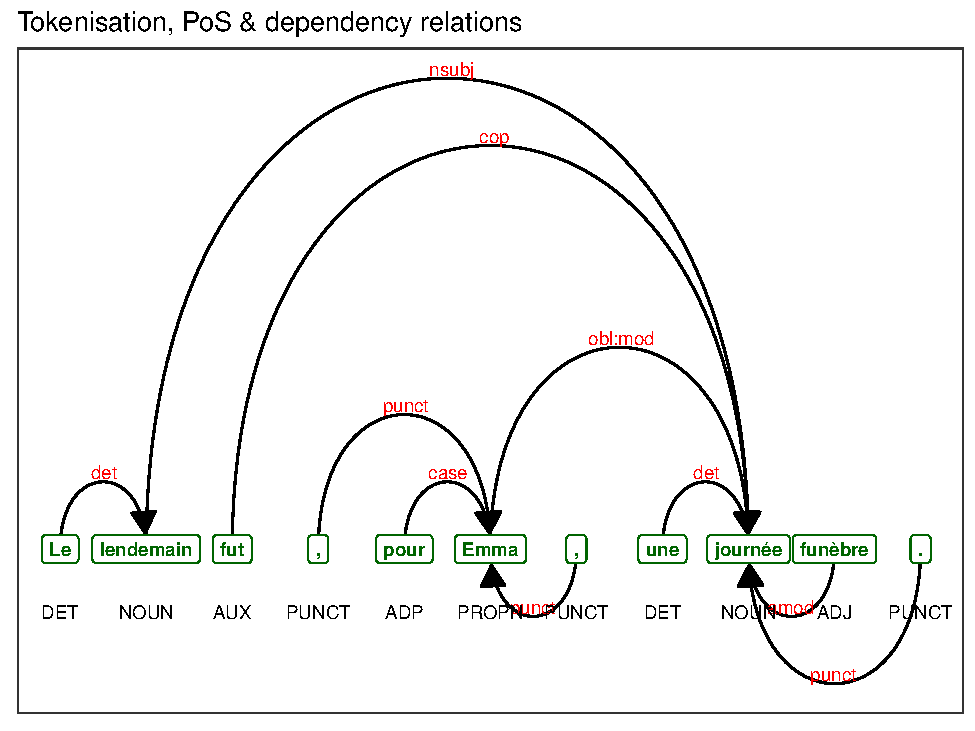
\includegraphics[width=0.8\linewidth]{bookdown-demo_files/figure-latex/72-1} 

}

\caption{arbre de dépendance}\label{fig:72}
\end{figure}

\hypertarget{vers-des-application-plus-guxe9nuxe9rale}{%
\subsection{Vers des application plus générale}\label{vers-des-application-plus-guxe9nuxe9rale}}

Dans la phrase precédente on note que funèbre est l'adjectif de journée. On peut être tenté de retrouver ces relations qui caractérisent des choses (les ``nouns'' ou noms choses) à des adjectifs. On souhaite faire une liste de ces paires.

L'exemple va être court : un poème de Maupassant

\begin{Shaded}
\begin{Highlighting}[]
\NormalTok{Maupassant<-Citations }\OperatorTok
\StringTok{  }\NormalTok{dplyr}\OperatorTok{::}\KeywordTok{filter}\NormalTok{(doc}\OperatorTok{==}\DecValTok{2}\NormalTok{)}

\NormalTok{UD <-}\StringTok{ }\KeywordTok{udpipe_annotate}\NormalTok{(udmodel_french, }\DataTypeTok{x=}\NormalTok{Maupassant}\OperatorTok{$}\NormalTok{text)}
\NormalTok{foo <-}\StringTok{ }\KeywordTok{as.data.frame}\NormalTok{(UD)}
\NormalTok{foo<-}\StringTok{ }\NormalTok{foo }\OperatorTok\StringTok{ }\KeywordTok{select}\NormalTok{(paragraph_id,sentence_id, token_id,lemma,upos,head_token_id,dep_rel)}\OperatorTok
\StringTok{  }\KeywordTok{mutate}\NormalTok{(}\DataTypeTok{key1=}\KeywordTok{paste0}\NormalTok{(paragraph_id,sentence_id, token_id),}\DataTypeTok{key2=}\KeywordTok{paste0}\NormalTok{(paragraph_id,sentence_id, head_token_id) )}
\end{Highlighting}
\end{Shaded}

On va donc construires un tableau lemme\_cible x lemmes\_associés, les premiers risqueront d'êtres les noms communs, les seconds leurs adjectifs.

\begin{Shaded}
\begin{Highlighting}[]
\CommentTok{# selection de la relation.}
\NormalTok{res <-}\StringTok{ }\NormalTok{foo }\OperatorTok\StringTok{ }\KeywordTok{filter}\NormalTok{(dep_rel }\OperatorTok{==}\StringTok{ "amod"}\NormalTok{)}
\CommentTok{#on y joint les dependences}
\NormalTok{dep<-res }\OperatorTok\StringTok{ }\KeywordTok{left_join}\NormalTok{(foo, }\DataTypeTok{by =} \KeywordTok{c}\NormalTok{(}\StringTok{"key2"}\NormalTok{ =}\StringTok{ "key1"}\NormalTok{))}

\CommentTok{#on construit la tables des relations lemmes cibles -adjectifs}
\NormalTok{table<-}\KeywordTok{as.data.frame.matrix}\NormalTok{(}\KeywordTok{table}\NormalTok{(dep}\OperatorTok{$}\NormalTok{lemma.x, dep}\OperatorTok{$}\NormalTok{lemma.y)) }
\CommentTok{#table$n<-rowSums(table)}
\CommentTok{#table$adj<-rownames(table)}
\CommentTok{#row.names(table) <- table$adj}
\end{Highlighting}
\end{Shaded}

le tableau obtenu est en fait la structure d'un graphe bipartite. la représentation passe par un de \texttt{igraph} avec pour paramètres importants :
* Taille des arcs (edge) : est proportionnelle à la force du lien ( nombre de relations)
* Taille des noeud : proportiennel au rangs du noeud.
* Couleur et forme des noeuds : lemme et lemme cible.
* Un algorithme de force de \citet{fruchterman_graph_1991} est employé pour représenter les positions relatives des mots et minimiser les superpositions.

Dessiner le réseau

\begin{Shaded}
\begin{Highlighting}[]
\NormalTok{bg <-}\KeywordTok{graph_from_incidence_matrix}\NormalTok{(table, }\DataTypeTok{weighted=}\OtherTok{TRUE}\NormalTok{)}
\KeywordTok{summary}\NormalTok{(bg)}
\end{Highlighting}
\end{Shaded}

\begin{verbatim}
## IGRAPH 518402e UNWB 36 20 -- 
## + attr: type (v/l), name (v/c), weight (e/n)
\end{verbatim}

\begin{Shaded}
\begin{Highlighting}[]
\CommentTok{#E(bg)$weight# See the vertex attributes }
\CommentTok{#V(bg)$type }
\CommentTok{#V(bg)$name}

\CommentTok{# Plot the network}
\NormalTok{shape =}\StringTok{ }\KeywordTok{ifelse}\NormalTok{(}\KeywordTok{V}\NormalTok{(bg)}\OperatorTok{$}\NormalTok{type, }\StringTok{"circle"}\NormalTok{, }\StringTok{"square"}\NormalTok{) }\CommentTok{# assign shape by node type}
\NormalTok{col =}\StringTok{ }\KeywordTok{ifelse}\NormalTok{(}\KeywordTok{V}\NormalTok{(bg)}\OperatorTok{$}\NormalTok{type, }\StringTok{"peachpuff"}\NormalTok{, }\StringTok{"darkolivegreen1"}\NormalTok{) }\CommentTok{# assign color by node type}
\KeywordTok{plot}\NormalTok{(bg, }\DataTypeTok{vertex.shape =}\NormalTok{ shape, }\DataTypeTok{vertex.label.cex=}\NormalTok{.}\DecValTok{9}\NormalTok{,}\DataTypeTok{vertex.label.color=}\StringTok{"black"}\NormalTok{,}\DataTypeTok{vertex.color =}\NormalTok{ col,}\DataTypeTok{edge.color=}\StringTok{"azure2"}\NormalTok{,}\DataTypeTok{vertex.frame.color=}\NormalTok{col, }\DataTypeTok{vertex.size=}\FloatTok{0.5}\OperatorTok{*}\NormalTok{igraph}\OperatorTok{::}\KeywordTok{degree}\NormalTok{(bg),}\DataTypeTok{layout=}\NormalTok{layout_with_fr,}\DataTypeTok{edge.width=}\DecValTok{1}\OperatorTok{*}\KeywordTok{E}\NormalTok{(bg)}\OperatorTok{$}\NormalTok{weight,}\DataTypeTok{edge.curved=}\FloatTok{0.5}\NormalTok{)}
\end{Highlighting}
\end{Shaded}


\includegraphics{bookdown-demo_files/figure-latex/75-1.pdf}

\hypertarget{reconnaissance-dentituxe9s-nommuxe9es}{%
\section{reconnaissance d'entités nommées}\label{reconnaissance-dentituxe9s-nommuxe9es}}

En français courant les entités nommées correspondent largement à l'idée de noms propres. Un nom propre à une entité. Une chose qui est est indépendemment des catégories qui peuvent l'étiqueter. John Dupont, né le 19 février 1898 à Glasgow et abattu à Verdun le 8 août 1917, est un personnage unique. John Dupont ne désigne par une catégorie, mais bien une personne singulière. La designation peut cependant être ambigüe, il y a un ``Paris, Texas.'', et un Paris sur Seine. La morphologie ne ressout pas l'ambiguité.

les entités nommées appartiennent à différentes catégories d'objets : des noms de lieux, des noms de personnes, des noms de marques, des acronymes d'organisation,

Elles ne représentent jamais une catégorie mais une unité singulière.

\url{https://cran.r-project.org/web/packages/nametagger/nametagger.pdf}

\hypertarget{co-refuxe9rence}{%
\section{co-reférence}\label{co-refuxe9rence}}

\hypertarget{analyse-du-sentiment}{%
\chapter{Analyse du sentiment}\label{analyse-du-sentiment}}

liu ping est le fondateur de l'analyse du sentiment et dès 2012 en donne une synthèse complète \citep{liu_sentiment_2012} . Depuis des développement considérables ont été apportée par des méthodes de deep learning, et notamment les modèles transformer et renouvvelent consirablement le domaine. On restra ici à un niveau classique ou compositionnel.

On travaillera sur un corpus d'avis trip advisor, sur la période avant co

\begin{Shaded}
\begin{Highlighting}[]
\NormalTok{df<-}\KeywordTok{readRDS}\NormalTok{(}\StringTok{"./data/AvisTripadvisor.rds"}\NormalTok{)}
\end{Highlighting}
\end{Shaded}

\hypertarget{un-exemple-avec-syuzhet}{%
\section{Un exemple avec syuzhet}\label{un-exemple-avec-syuzhet}}

On utilise le package \href{https://www.rdocumentation.org/packages/syuzhet/versions/1.0.4}{syuzhet} et en particulier le dictionnaire ``nrc'' developpé et traduit par \citet{mohammad_crowdsourcing_2013} ( Index Feel)

Le même outil fournit un autre systéme d'annotation qui compte les mentions d'éléments positifs ou négatifs, ainsi que d'émotions définies sur la base de l'inventaire de \citet{plutchik_psychoevolutionary_1982} on utilise simplement la fonction \texttt{get\_nrc\_sentiment}, en précisant le dictionnaire adéquat. L'échelle comprend en fait deux éléments : les 8 émotion de base *au sens de pluchik, et deux indicateurs de polarité.
L'opérationnalisation réalisée par \citet{mohammad_crowdsourcing_2013} s'inscrit dans une tradition de la recherche en marketing, se souvenir de \citet{havlena_varieties_1986} et de \citet{westbrook_dimensionality_1991}.

\begin{Shaded}
\begin{Highlighting}[]
\KeywordTok{library}\NormalTok{(syuzhet)             }\CommentTok{#analyse du sentimeent}

\CommentTok{#paramétres}
\NormalTok{method <-}\StringTok{ "nrc"}
\NormalTok{lang <-}\StringTok{ "french"}
\NormalTok{phrase<-}\KeywordTok{as.character}\NormalTok{(}\KeywordTok{paste0}\NormalTok{(df}\OperatorTok{$}\NormalTok{Titre,}\StringTok{" "}\NormalTok{,df}\OperatorTok{$}\NormalTok{Commetaire))}
\CommentTok{#extraction}

\NormalTok{emotions <-}\StringTok{ }\KeywordTok{get_nrc_sentiment}\NormalTok{(phrase,}\DataTypeTok{language =} \StringTok{"french"}\NormalTok{)}
\NormalTok{polarity<-}\KeywordTok{subset}\NormalTok{(emotions,}\DataTypeTok{select=}\KeywordTok{c}\NormalTok{(positive, negative))}
\NormalTok{df<-}\KeywordTok{cbind}\NormalTok{(df,polarity)}
\end{Highlighting}
\end{Shaded}

On s'intéresse surtout aux mentions positives et négatives (les émotions c'est pour plus tard. (la mesure permet ainsi une dissymétrie des deux polarités, il y a le bien, le mal, le mal et le bien, mais aussi si qui n'est ni mal ni bien).
Les textes étant inégaux en taille on va ramener l'indicateur de polarité au nombre de caractéres (sur une base de 500 c) de chaque contribution. En effet l'algo compte les valence et leur intensité est proportionnel à la longueur du texte. Ce qui est clairement démontré par la seconde figure.

A partir de ces deux mesures, 4 indicateurs peuvent étre construits
* Positivité : nombre de termes positifs pour 500 signes.
* Négativitivé : nombre de termes négatifs pour 500 signes.
* Valence : rapport du nombre de termes positifs sur les négatifs.
* Expressivité : nombre de termes positifs et négatifs.
le dernier graphe nous apprend que les jugements plutôt positifs sont aussi les plus expressifs. La ``froideur'' des avis les plus négatifs refléte-t-elle une crainte de la désaprobation sociale. C'est une piste de recherche à poursuivre, on pourrait s'attendre à ce que les avis les plus négatifs surgissent plus facilement si la densité des négatives est plus importante et observer une sorte d'autocorrélation.

\begin{Shaded}
\begin{Highlighting}[]
\NormalTok{G1<-}\KeywordTok{ggplot}\NormalTok{(df, }\KeywordTok{aes}\NormalTok{(}\DataTypeTok{x=}\NormalTok{positive))}\OperatorTok{+}\KeywordTok{geom_histogram}\NormalTok{(}\DataTypeTok{binwidth =} \DecValTok{1}\NormalTok{, }\DataTypeTok{fill=}\StringTok{"darkred"}\NormalTok{)}\OperatorTok{+}\KeywordTok{theme_minimal}\NormalTok{()}
\NormalTok{G1}
\end{Highlighting}
\end{Shaded}

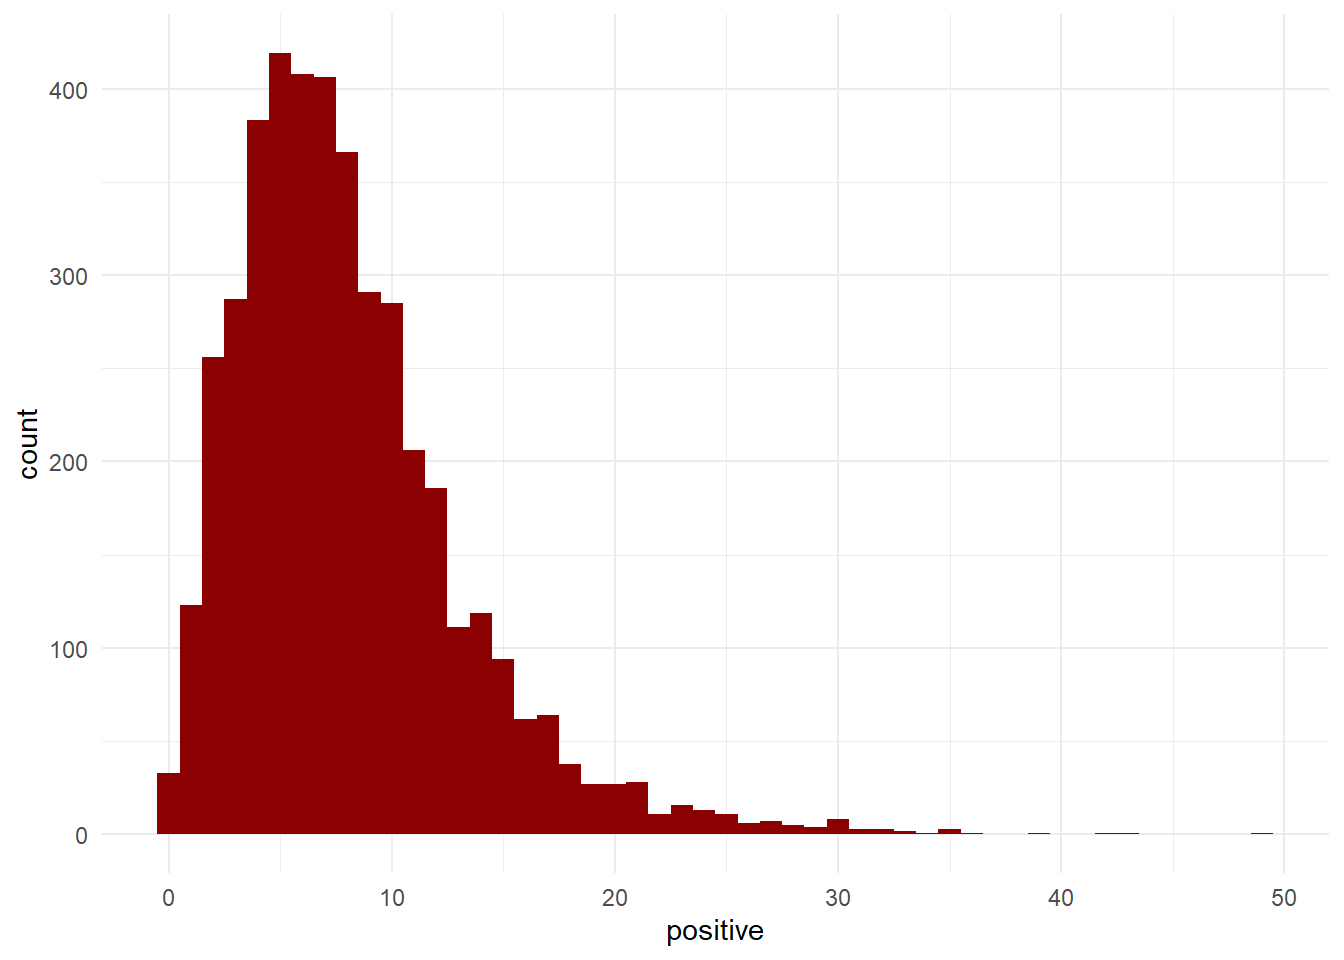
\includegraphics{bookdown-demo_files/figure-latex/63-1.pdf}

\begin{Shaded}
\begin{Highlighting}[]
\NormalTok{G2<-}\KeywordTok{ggplot}\NormalTok{(df, }\KeywordTok{aes}\NormalTok{(}\DataTypeTok{x=}\NormalTok{negative))}\OperatorTok{+}\KeywordTok{geom_histogram}\NormalTok{(}\DataTypeTok{binwidth =} \DecValTok{1}\NormalTok{,}\DataTypeTok{fill=}\StringTok{"Royalblue"}\NormalTok{)}\OperatorTok{+}\KeywordTok{theme_minimal}\NormalTok{()}
\NormalTok{G2}
\end{Highlighting}
\end{Shaded}

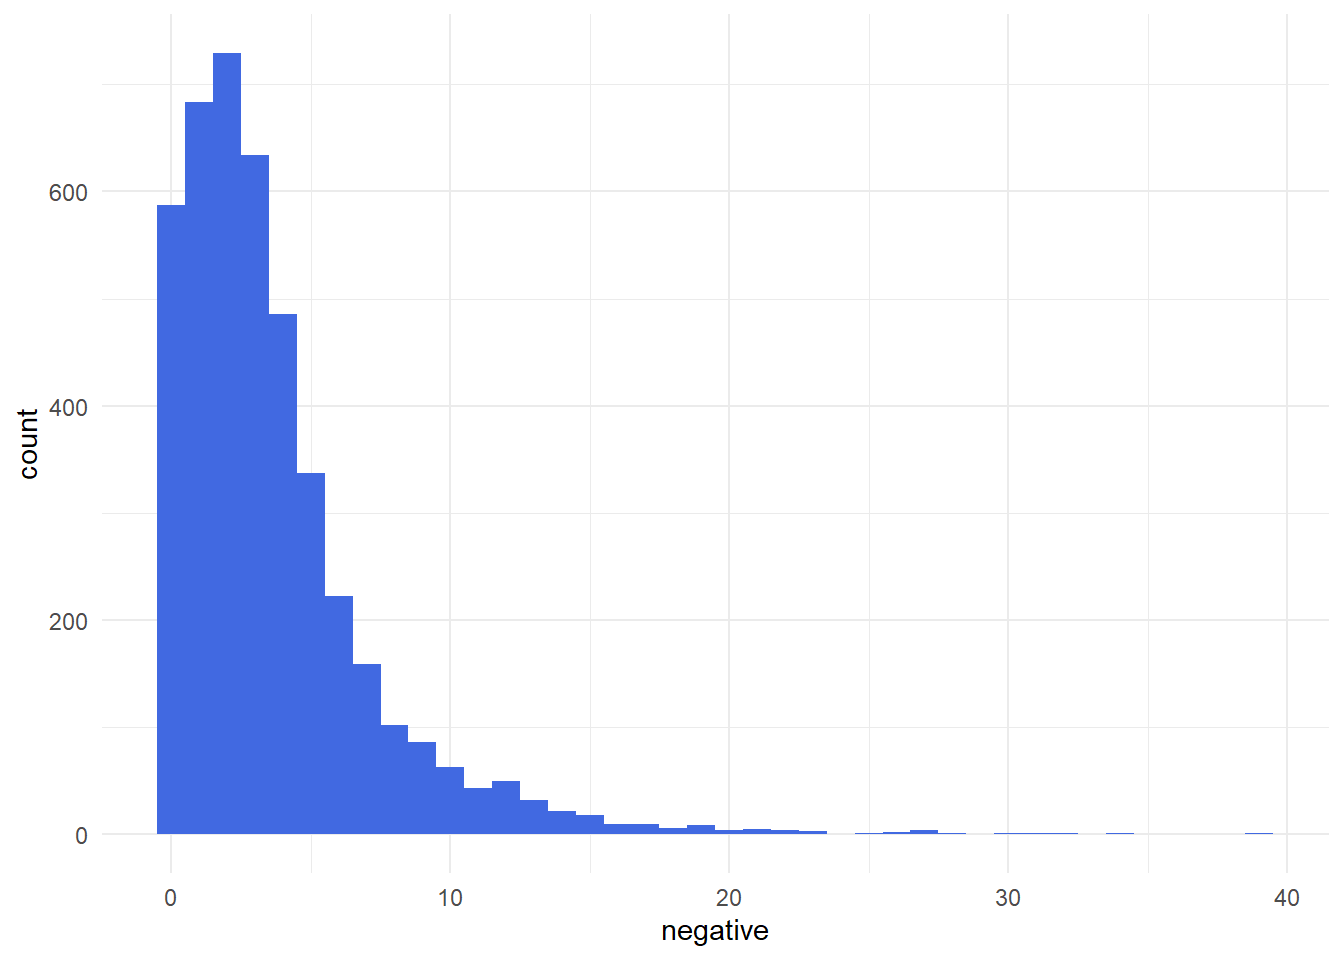
\includegraphics{bookdown-demo_files/figure-latex/63-2.pdf}

\hypertarget{valence-et-expression}{%
\subsection{Valence et expression}\label{valence-et-expression}}

la linguistique donne aux mots une valence : elle peut être positive (bonheur), négative (malheur) ou neutre ( tranquité).

C'est un régime ternaire. Chaque mot d'une phrase est neutre, positif ou négatif.

On peut doser les effets

On a des dictionnaires

\begin{Shaded}
\begin{Highlighting}[]
\NormalTok{df}\OperatorTok{$}\NormalTok{text<-}\KeywordTok{as.character}\NormalTok{(}\KeywordTok{paste0}\NormalTok{(df}\OperatorTok{$}\NormalTok{Titre,}\StringTok{" "}\NormalTok{,df}\OperatorTok{$}\NormalTok{Commetaire))}
\NormalTok{df}\OperatorTok{$}\NormalTok{WC<-}\KeywordTok{str_count}\NormalTok{(df}\OperatorTok{$}\NormalTok{text, }\StringTok{"}\CharTok{\textbackslash{}\textbackslash{}}\StringTok{S+"}\NormalTok{)}

\NormalTok{df}\OperatorTok{$}\NormalTok{positivity<-(df}\OperatorTok{$}\NormalTok{positive)}\OperatorTok{/}\NormalTok{(df}\OperatorTok{$}\NormalTok{WC)}
\NormalTok{df}\OperatorTok{$}\NormalTok{negativity<-(df}\OperatorTok{$}\NormalTok{negative)}\OperatorTok{/}\NormalTok{(df}\OperatorTok{$}\NormalTok{WC)}
\NormalTok{df}\OperatorTok{$}\NormalTok{valence<-df}\OperatorTok{$}\NormalTok{positivity}\OperatorTok{-}\NormalTok{df}\OperatorTok{$}\NormalTok{negativity}
\NormalTok{df}\OperatorTok{$}\NormalTok{expressivity<-df}\OperatorTok{$}\NormalTok{positivity}\OperatorTok{+}\NormalTok{df}\OperatorTok{$}\NormalTok{negativity}

\NormalTok{G11<-}\KeywordTok{ggplot}\NormalTok{(df, }\KeywordTok{aes}\NormalTok{(}\DataTypeTok{x=}\NormalTok{valence,}\DataTypeTok{y=}\NormalTok{expressivity ))}\OperatorTok{+}\KeywordTok{geom_point}\NormalTok{(}\DataTypeTok{color=}\StringTok{"grey"}\NormalTok{)}\OperatorTok{+}\KeywordTok{geom_smooth}\NormalTok{(}\DataTypeTok{method =} \StringTok{"gam"}\NormalTok{, }\DataTypeTok{formula =}\NormalTok{ y }\OperatorTok{~}\StringTok{ }\KeywordTok{s}\NormalTok{(x, }\DataTypeTok{bs =} \StringTok{"cs"}\NormalTok{))}\OperatorTok{+}\KeywordTok{theme_minimal}\NormalTok{()}
\NormalTok{G12<-}\KeywordTok{ggplot}\NormalTok{(df, }\KeywordTok{aes}\NormalTok{(}\DataTypeTok{x=}\NormalTok{negativity,}\DataTypeTok{y=}\NormalTok{positivity ))}\OperatorTok{+}\KeywordTok{geom_point}\NormalTok{(}\DataTypeTok{color=}\StringTok{"grey"}\NormalTok{)}\OperatorTok{+}\KeywordTok{geom_smooth}\NormalTok{(}\DataTypeTok{method =} \StringTok{"gam"}\NormalTok{, }\DataTypeTok{formula =}\NormalTok{ y }\OperatorTok{~}\StringTok{ }\KeywordTok{s}\NormalTok{(x, }\DataTypeTok{bs =} \StringTok{"cs"}\NormalTok{))}\OperatorTok{+}\KeywordTok{theme_minimal}\NormalTok{()}
\NormalTok{G13<-}\KeywordTok{ggplot}\NormalTok{(df, }\KeywordTok{aes}\NormalTok{(}\DataTypeTok{x=}\NormalTok{negativity,}\DataTypeTok{y=}\NormalTok{ expressivity))}\OperatorTok{+}\KeywordTok{geom_point}\NormalTok{(}\DataTypeTok{color=}\StringTok{"grey"}\NormalTok{)}\OperatorTok{+}\KeywordTok{geom_smooth}\NormalTok{(}\DataTypeTok{method =} \StringTok{"gam"}\NormalTok{, }\DataTypeTok{formula =}\NormalTok{ y }\OperatorTok{~}\StringTok{ }\KeywordTok{s}\NormalTok{(x, }\DataTypeTok{bs =} \StringTok{"cs"}\NormalTok{))}\OperatorTok{+}\KeywordTok{theme_minimal}\NormalTok{()}
\NormalTok{G14<-}\KeywordTok{ggplot}\NormalTok{(df, }\KeywordTok{aes}\NormalTok{(}\DataTypeTok{x=}\NormalTok{positivity,}\DataTypeTok{y=}\NormalTok{ expressivity))}\OperatorTok{+}\KeywordTok{geom_point}\NormalTok{(}\DataTypeTok{color=}\StringTok{"grey"}\NormalTok{)}\OperatorTok{+}\KeywordTok{geom_smooth}\NormalTok{(}\DataTypeTok{method =} \StringTok{"gam"}\NormalTok{, }\DataTypeTok{formula =}\NormalTok{ y }\OperatorTok{~}\StringTok{ }\KeywordTok{s}\NormalTok{(x, }\DataTypeTok{bs =} \StringTok{"cs"}\NormalTok{))}\OperatorTok{+}\KeywordTok{theme_minimal}\NormalTok{()}

\KeywordTok{plot_grid}\NormalTok{(G11, G12, G13,G14, }\DataTypeTok{labels =} \KeywordTok{c}\NormalTok{(}\StringTok{'A'}\NormalTok{, }\StringTok{'B'}\NormalTok{, }\StringTok{'C'}\NormalTok{,}\StringTok{'D'}\NormalTok{))}
\end{Highlighting}
\end{Shaded}

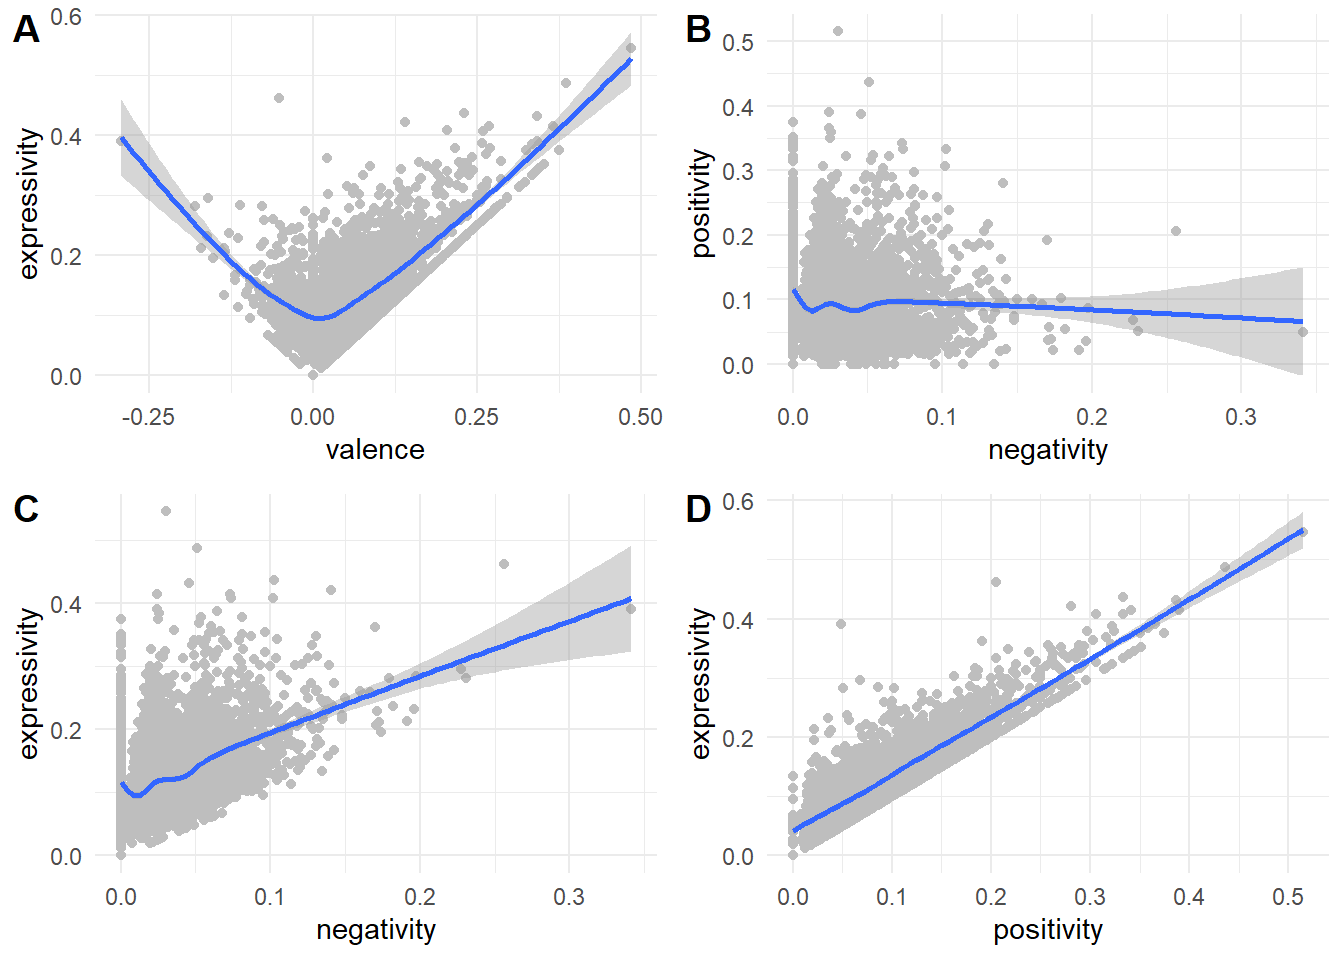
\includegraphics{bookdown-demo_files/figure-latex/64-1.pdf}

\hypertarget{la-guxe9nuxe9ralisation-par-le-liwc}{%
\section{La généralisation par le Liwc}\label{la-guxe9nuxe9ralisation-par-le-liwc}}

Le liwc vient de l'idée simple d'un psychiatre qui a souhaité faire des diagnoistics de trauma craniens à partir des entretiens menés avec lmes patients atteints. \citep{tausczik_psychological_2010}

Le LIWC permet d'obtenir d'autres indicateurs du sentiment, une partie des 80 indicateurs proposés est relatif à des dimensions topicales dont trois groupes vont retenir notre attention dans la mesure où ils décrivent une partie de l'expérience relatée dans les commentaires.
* La sensorialité ( voir, entendre, sentir)
* L'orientation temporelle ( passé, présent, futur)
* les émotions négatives (tristesse, colére, )

La procédure pour extraire ces notions est fort simple . On utilise l'infrasturure de quanteda et une version francophone du dictionnaire \citep{piolat_version_2011}

\begin{Shaded}
\begin{Highlighting}[]
\CommentTok{# the devtools package needs to be installed for this to work}
\CommentTok{#devtools::install_github("kbenoit/quanteda.dictionaries")}
\KeywordTok{library}\NormalTok{(cleanNLP)}
\KeywordTok{library}\NormalTok{(}\StringTok{"quanteda.dictionaries"}\NormalTok{)}
\NormalTok{dict_liwc_french <-}\StringTok{ }\KeywordTok{dictionary}\NormalTok{(}\DataTypeTok{file =} \StringTok{"FrenchLIWCDictionary.dic"}\NormalTok{,}
                             \DataTypeTok{format =} \StringTok{"LIWC"}\NormalTok{)}
\NormalTok{test<-}\KeywordTok{liwcalike}\NormalTok{(df}\OperatorTok{$}\NormalTok{Commetaire,}\DataTypeTok{dictionary =}\NormalTok{ dict_liwc_french)}
\NormalTok{df<-}\KeywordTok{cbind}\NormalTok{(df,test)}
\end{Highlighting}
\end{Shaded}

\hypertarget{encore-dautres-guxe9nuxe9ralisations}{%
\section{Encore d'autres généralisations}\label{encore-dautres-guxe9nuxe9ralisations}}

L'approche par dictionnaire s'est déplacée vers l'identification d'autre catégorie

\begin{itemize}
\tightlist
\item
  les valeurs morales
\end{itemize}

\hypertarget{construire-son-propre-dictionnaire}{%
\section{construire son propre dictionnaire}\label{construire-son-propre-dictionnaire}}

faire des listes de lmots

\hypertarget{le-retour-des-muxe9thodes-factorielles}{%
\chapter{Le retour des méthodes factorielles}\label{le-retour-des-muxe9thodes-factorielles}}

D'un point de vue historique l'analyse factorielle est une idées de psychologue. D'ailleur un des meilleurs packages jamais développé est sans doute psych

L'école française a choisit l'ACP, et ses dérivée appliquées à des données de comptage comme l'AFCM.

Ces méthodes s'appuient sur des techniques de décomposition de matrice, et vise à réduire leur rang. Le problèmes qu'elle cherchent à résoudre est de réduire l'espace d'information.

\hypertarget{retour-sur-lacp}{%
\section{Retour sur l'ACP}\label{retour-sur-lacp}}

L'ACP a été longtemps la méthode reine, elle est toujours fréquemmment utilisées.Elle vise à un but simple : représenter un ensemble de donnée comportant k variable à un petit nombre de combinaisons de ces variables qui représentent une grandes part de l'information.

Historiquement elle a été développée pour analyser des matrices de corrélations multiples où X est une matrice de n individus et k variables ou mesure. Dans le domain textuel ce tableau correspond au dtm où les individus sont les documents et les colonnes les termes.

\(\Sigma=X*X^\top\)

L'idée principale est de trouver des combinaisons linéaires des variables qui capture succéssivement une part maximale de la variance. La solution à ce problème revient à décomposer cette matrice en fonction d'un matrice de poids qui est determinée comme la matrice des valeur propre de \(\Sigma\).

\(\Sigma=F*V*F^\top\)

\url{https://fr.wikipedia.org/wiki/Jean-Paul_Benz\%C3\%A9cri}

\url{https://www.math3ma.com/blog/understanding-entanglement-with-svd}

X=FSF

\hypertarget{svd}{%
\section{SVD}\label{svd}}

quelle différence avec PCA

\url{https://stats.stackexchange.com/questions/134282/relationship-between-svd-and-pca-how-to-use-svd-to-perform-pca}

\hypertarget{lsa}{%
\section{LSA}\label{lsa}}

\hypertarget{nlm}{%
\section{NLM}\label{nlm}}

\hypertarget{vectorisation-du-corpus}{%
\chapter{Vectorisation du corpus}\label{vectorisation-du-corpus}}

\hypertarget{word2vec}{%
\section{Word2vec}\label{word2vec}}

\hypertarget{vectorisation-pipe}{%
\subsection{vectorisation pipe}\label{vectorisation-pipe}}

\hypertarget{closest2}{%
\subsection{closest2}\label{closest2}}

\hypertarget{map-with-tsne}{%
\subsection{map with tsne}\label{map-with-tsne}}

\hypertarget{paragraph2vec}{%
\section{paragraph2vec}\label{paragraph2vec}}

\hypertarget{lavenir-des-moduxe8les-pruxe9-entrainuxe9s}{%
\section{l'avenir des modèles pré-entrainés}\label{lavenir-des-moduxe8les-pruxe9-entrainuxe9s}}

\hypertarget{topic-analysis}{%
\chapter{Topic Analysis}\label{topic-analysis}}

\hypertarget{lda}{%
\section{LDA}\label{lda}}

\hypertarget{le-moduxe8le-de-blei}{%
\subsection{le modèle de blei}\label{le-moduxe8le-de-blei}}

\hypertarget{implementation-avec-wor2vec}{%
\subsection{implementation avec wor2vec}\label{implementation-avec-wor2vec}}

\hypertarget{repruxe9sentation-graphique}{%
\subsection{Représentation graphique}\label{repruxe9sentation-graphique}}

\hypertarget{la}{%
\subsection{La}\label{la}}

\hypertarget{stm}{%
\section{STM}\label{stm}}

\hypertarget{section}{%
\subsection{}\label{section}}

\hypertarget{section-1}{%
\subsection{}\label{section-1}}

\hypertarget{machine-learning-with-text}{%
\chapter{Machine learning with text}\label{machine-learning-with-text}}

\hypertarget{simples-models}{%
\section{simples models}\label{simples-models}}

\hypertarget{naives-bayes}{%
\subsection{Naives bayes}\label{naives-bayes}}

\hypertarget{elastic-net}{%
\subsection{elastic net}\label{elastic-net}}

\hypertarget{rf}{%
\subsection{RF}\label{rf}}

\hypertarget{art-of-featuring}{%
\section{art of featuring}\label{art-of-featuring}}

utiliser les plongements

\hypertarget{deep-learning}{%
\chapter{Deep Learning}\label{deep-learning}}

Pour l'utilisateur en sciences sociales même si le deep learning est accessible dans un environnement r, et nous examinerons les possibilités offerte par kera, constuire son modèle de langage est sans doute hors de portée. Il s'agira donc le plus souvent d'employer des modèles pré-entrainés, et éventuellement de les réentrainer sur nos coprus de données.

\hypertarget{lenvironnement-keras}{%
\section{L'environnement keras}\label{lenvironnement-keras}}

l'interface de r pour \href{https://keras.rstudio.com/}{Keras}

\hypertarget{les-fonctions-principales}{%
\subsection{Les fonctions principales}\label{les-fonctions-principales}}

\begin{itemize}
\item
  cpu et gpu
\item
\end{itemize}

\hypertarget{un-premier-exemple}{%
\subsection{Un premier exemple}\label{un-premier-exemple}}

lequel?

\hypertarget{un-deuxiuxe8me-exemple}{%
\subsection{Un deuxième exemple}\label{un-deuxiuxe8me-exemple}}

Lequel?

\hypertarget{les-architectures-du-texte-rnn-ltsm-transformer-et-reformer}{%
\section{Les architectures du texte : RNN, LTSM, Transformer et reformer}\label{les-architectures-du-texte-rnn-ltsm-transformer-et-reformer}}

Les évolutions de ces 10 dernières années se caractèreisent par la recherche d'architectures qui prennent en comptent la structure du texte : il y a un ordre séquentiel : les mots font sens quand on les lis ou les entends après une succision d'ordre mots dont on connait les règles de composition.

\hypertarget{rnn}{%
\subsection{rnn}\label{rnn}}

Il était logique que les rnn soient la première architecture qui a rendu des résultats intéressants. Leur acaractère autorégressif

\hypertarget{ltsm}{%
\subsection{ltsm}\label{ltsm}}

Les ltsm on apportant une amélioration en prenant en compte des coorélations immédiates mais aussi plus lointaine dans le régl\&age de l'oubli et de la mémoire

\hypertarget{transformer}{%
\subsection{transformer}\label{transformer}}

L'innovation des transformer, fondée sur des modèles a trou\ldots..

\hypertarget{reformer}{%
\subsection{reformer}\label{reformer}}

Les reformer étendent l'échelle des corrélations possibles. Parfois ce qui donne le sens d'un texte après 500 mots est peut \_être le premier, même si nous ne l'ons pas perçu, il devient le contexte de la chute par exemple.

exemple?

\hypertarget{les-cas-dapplications-remarquables}{%
\section{Les cas d'applications remarquables}\label{les-cas-dapplications-remarquables}}

\hypertarget{detection-dintention}{%
\subsection{Detection d'intention}\label{detection-dintention}}

quand la théorie des actes de langages rencontre l'informatique

\hypertarget{duxe9tection-de-toxicituxe9-des-contenus}{%
\subsection{détection de toxicité des contenus}\label{duxe9tection-de-toxicituxe9-des-contenus}}

\hypertarget{la-detection-des-trolls}{%
\subsection{la detection des trolls}\label{la-detection-des-trolls}}

\hypertarget{duxe9tection-des-sophismes-et-autres-fallacies}{%
\subsection{détection des sophismes et autres fallacies}\label{duxe9tection-des-sophismes-et-autres-fallacies}}

la lutte anti fake

\hypertarget{la-duxe9tection-du-sarcasme-et-de-lironie}{%
\subsection{La détection du sarcasme et de l'ironie}\label{la-duxe9tection-du-sarcasme-et-de-lironie}}

\hypertarget{lextraction-dargumennts}{%
\subsection{L'extraction d'argumennts}\label{lextraction-dargumennts}}

triplet

\hypertarget{translation}{%
\chapter{Translation}\label{translation}}

\hypertarget{simples-models-1}{%
\section{simples models}\label{simples-models-1}}

\hypertarget{naives-bayes-1}{%
\subsection{Naives bayes}\label{naives-bayes-1}}

\hypertarget{elastic-net-1}{%
\subsection{elastic net}\label{elastic-net-1}}

\hypertarget{rf-1}{%
\subsection{RF}\label{rf-1}}

\hypertarget{art-of-featuring-1}{%
\section{art of featuring}\label{art-of-featuring-1}}

utiliser les plongements

\hypertarget{moduxe8les-guxe9nuxe9ratifs}{%
\chapter{Modèles génératifs}\label{moduxe8les-guxe9nuxe9ratifs}}

\hypertarget{simples-models-2}{%
\section{simples models}\label{simples-models-2}}

\hypertarget{naives-bayes-2}{%
\subsection{Naives bayes}\label{naives-bayes-2}}

\hypertarget{elastic-net-2}{%
\subsection{elastic net}\label{elastic-net-2}}

\hypertarget{rf-2}{%
\subsection{RF}\label{rf-2}}

\hypertarget{art-of-featuring-2}{%
\section{art of featuring}\label{art-of-featuring-2}}

utiliser les plongements

\hypertarget{annexes-quelques-probluxe8mes-truxe8s-techniques}{%
\chapter{Annexes : quelques problèmes très techniques}\label{annexes-quelques-probluxe8mes-truxe8s-techniques}}

\hypertarget{la-question-de-lencodage}{%
\section{La question de l'encodage}\label{la-question-de-lencodage}}

Le lecteur sera soumis très rapidement au problème compliqué et agaçant de l'encodage des données.

\hypertarget{jouer-avec-les-formats-de-donnuxe9es}{%
\section{Jouer avec les formats de données}\label{jouer-avec-les-formats-de-donnuxe9es}}

Le modèle excell appartient au passé
\#\#\# json
Le jason et la logique des liste
\#\#\# xml
l'xml triomphant

\hypertarget{des-formats-exotiques}{%
\subsection{des formats exotiques}\label{des-formats-exotiques}}

ris et bib pour la biblio

\hypertarget{adopter-des-formats-propres-tidy}{%
\section{Adopter des formats ``propres'' (tidy)}\label{adopter-des-formats-propres-tidy}}

\hypertarget{les-limites-du-calcul}{%
\section{Les limites du calcul}\label{les-limites-du-calcul}}

Certaines opérations sont couteuse en calcul, notamment l'annotation.

calculer les temps de calculs

parralélisation

optimisation

  \bibliography{book.bib,packages.bib}

\end{document}
